

%%% Local Variables:
%%% mode: latex
%%% TeX-master: t
%%% End:

\documentclass[11pt,a4paper,english]{book}
\usepackage{amsmath}
\usepackage{ae}
\usepackage[english, USenglish]{babel}
%\usepackage[latin1]{inputenc}
\usepackage[utf8x]{inputenc}
\usepackage{ucs} % unicode
\usepackage[T1]{fontenc}
\usepackage{t1enc}
\usepackage{type1cm}
%\usepackage{mathptmx}
%\usepackage[scaled=0.9]{helvet}
%\usepackage{courier}
\usepackage{graphicx}
\usepackage{natbib}
\usepackage{rotating}

% Thanks to Daniel Ferrante
% http://olympus.het.brown.edu/~danieldf/latex/
% \usepackage{eso-pic}
% \usepackage{color}
% \makeatletter
%   \AddToShipoutPicture{%
%     \setlength{\@tempdimb}{.5\paperwidth}%
%     \setlength{\@tempdimc}{.5\paperheight}%
%     \setlength{\unitlength}{1pt}%
%     \put(\strip@pt\@tempdimb,\strip@pt\@tempdimc){%
%       \makebox(0,0){\rotatebox{45}{\textcolor[gray]{0.75}{\fontsize{5cm}{5cm}\selectfont{Draft}}}}
%     }
% }
% \makeatother

\pagestyle{myheadings}

\sloppy

\begin{document}

%\fontsize{12}{18}
%\selectfont

\title{Das Schlusskapitel aus: "`Explaining Altruism. A Simulation-Based Approach and its
Limits"'}

\author{Eckhart Arnold}
\date{January 2008}

\maketitle


\begin{flushright}
{\small Die Wissenschaft denkt nicht.\\{\em Heidegger}} 
\end{flushright}

\thispagestyle{empty}
\noindent
\vspace{10cm}

% Ich erkläre hiermit, dass ich die vorliegende Arbeit ohne Hilfe Dritter und
% ohne Benutzung anderer als der angegebenen Hilfsmittel angefertigt habe; die
% aus fremden Quellen (einschließlich des Internets) direkt oder indirekt
% übernommenen Gedanken sind als solche kenntlich gemacht.
% 
% Die Arbeit wurde bisher in gleicher oder ähnlicher Form keiner anderen
% Prüfungsbehörde vorgelegt. 

%\pagenumbering{roman}
\tableofcontents

%\nocite{*} 

%\setcounter{page}{1}
%\pagenumbering{arabic}

%

\chapter{Introduction}

\pagenumbering{arabic}
\setcounter{page}{7}

In this book I examine evolutionary explanations of altruism that are based
on computer simulations. When speaking of {\em explanations} of
altruism, this means that this book is not primarily a study that tries to explain
altruism itself, but a critical examination of how these explanations work.
Its aim is twofold: On the one hand, it will expound this type of
explanations of altruism, describe its working mechanisms and the results that
can be obtained. In this respect this book strongly draws on the simulation
based approach to the evolution of altruism that was pioneered by Robert
Axelrod and William D. Hamilton \cite[]{axelrod-hamilton:1981} and made
popular through Axelrod's book on ``The Evolution of Cooperation''
\cite[]{axelrod:1984}. However, after the more than twenty years that have
passed since the publication of this book, the fact can hardly be ignored that
the simulation-based approach to the explanation of altruism did not quite
live up to the very expectations and aspirations that it once gave rise to and
to the ``simulation hype'' it caused. Therefore, this book will on the other
hand broadly discuss the limits of this approach. My aim is to give a
clear diagnosis of this failure, to explain why this approach remained largely
unsuccessful and also to point out what lessons regarding the research design of
computer simulations can be learned in order to allow a more purposeful employment of computer simulations for scientific explanations in the future.

In this introduction, I first say a few words about the topic and
theoretical background that is, about why the evolution of altruism is a topic
that interests us, why an evolutionary approach may be suitable to tackle the
question of altruism and, finally, how computer simulations come into play
here. Then, I briefly explain my method for examining the simulation-based evolutionary explanations of altruism and its alleged failure.
Basically, my method consists in conducting some simulations in the common
fashion of this approach myself and looking at the corresponding empirical
research both in biology and in the social sciences. I also give in this
introduction a very brief overview of the main results of my inquiry.
Finally, I present the structuring of this book and, in this context,
further describe the methodological decisions I have taken.

\section{The explanation of altruism as a scientific problem}

The explanation of altruism poses an intriguing riddle both in biology and in
the social sciences. In biology the question is how, if ``survival of the
fittest'' is the rule, altruistic behavioral traits can evolve when altruism
means by definition the giving-up of some of an organism's own fitness in
order to increase the fitness of another organism. Yet, as ants, honeybees or
the behavior of brood care in almost any species testify, altruism does exist
in nature. How then, did it arise?

Similarly, while we all believe that humans are moral creatures that can by
proper education and appropriate incentives learn to behave as altruists, the
question still remains why, if -- as we observe in many areas of life --
egoism is the road to success, altruistic norms should continue to enjoy a
high and general esteem. Should not a lack of secular success of the adherents
of altruistic norms mark such norms as unrealistic if not foolish?

Moreover, altruism raises not only important questions in the empirical
sciences, but also for moral philosophy and metaphysics.  For, when we
postulate altruistic moral norms we surely want to know (if we are not pure
{\em Gesinnungsethiker}) whether and to what degree we can realistically
expect obedience to these norms. From a metaphysical perspective the question
of the viability of altruism links to the old question of whether the world as
a whole is good or bad and, if bad, whether it can be made any better or if we
will have to cope with the fact that ``the realm of virtue is not from this
earth'' \cite[]{schopenhauer:1831}.

Thus, the existence of altruism demands an explanation and the desirability of
altruism calls for an understanding of the circumstances under which altruism
can flourish. In this book an examination will be made as to what an
evolutionary simulation-based approach can contribute to the understanding of
altruism.

\section{Method and central theses}

Why use an evolutionary approach for the explanation of altruism? In biology
the answer to this question is obvious: Any phenotypic trait of any organism
must -- according to Darwin's theory of evolution -- have evolved through
natural selection. If a certain organism or species exposes an altruistic
behavioral trait then there must be an evolutionary explanation for it. The
situation is different in the social sciences.  As is usual in the social
sciences there exist many competing paradigms upon which a scientist could
draw in order to explain the genesis of social norms, including norms that
prescribe altruistic conduct. The evolutionary theory of culture which seeks
to apply the principles of the Darwinian theory of evolution (reproduction,
variation, selection) to the evolution of cultural traits is a comparatively
young contender. Its practical value for the social sciences is still
disputed\footnote{See Bryant \cite[]{bryant:2004} for a fundamental criticism
  of the evolutionary theory of culture.}  and, due to the fact that there exist
many good alternative explanations for cultural developments, it would
be too much to expect that the evolutionary theory of culture could repeat in
the social sciences the very success that Darwinism had in biology. Yet, there are
some good points in favor of it. First of all, the evolutionary theory of
culture may prove able to explain things that other theories of cultural
developments cannot explain.\footnote{See Arnold \cite[]{arnold:2002} for some
  speculations on this topic.} Then, where it proves able to explain cultural
developments, it most probably can provide general patterns of explanation
that can be applied both in biology and in social sciences.
% \footnote{I am
%   speaking here of ``patterns of explanation'' instead of just
%   ``explanations'' because the generality of these patterns lies on a purely
%   epistemic level.  Ontologically, genetic evolution in biology and cultural
%   evolution in the social sciences relate to a different set of causes. Only,
%   the same or very similar abstract models of evolutionary processes may be
%   applied in both areas.} 
If the evolutionary theory of culture should prove
to be successful then it could be regarded as a great advance in terms of the
economy of knowledge. Finally, explanatory patterns that cover different areas
of research may profit from synergistic effects, which means that an
advancement of modeling or empirical research in one of the fields may carry
over to the other fields.

However, there are also downsides to such a generalizing approach.  Most
notably there is the danger of overlooking peculiarities of the respective
areas of research and, as always with generalizing, there is the danger of
oversimplification. Ultimately, the choice to use an evolutionary approach to
study altruism is -- as far as the social sciences are concerned -- to some
degree a matter of preference and motivated by the desire to find an
explanation for altruism as broad as possible.

Given that it has been decided to use an evolutionary approach to study
altruism the next question would be why computer simulations should be
employed to furnish the evolutionary research on altruism.  In principle,
there would be four different alternatives: 1) One could rely on purely verbal
reasoning to explain the evolution of altruism.  But then, verbal evolutionary
explanations tend to be notoriously weak. It is almost always possible to
construct some sort of evolutionary story of why some certain trait had to
evolve and often it is just as easy to explain on the same level why its
opposite should have evolved (even if in fact it did not) if only because it
is usually easy to feign some plausible selective conditions under which the
trait in question would be advantageous. 2) Another alternative is
mathematical modeling. It allows -- as one should presume -- for a very
precise expression of the concepts in question, but it can easily become
extremely complicated and tedious, once it rises above the mere expression of
the concept of, say, reciprocal altruism to models that can halfway
realistically depict a situation in the real world where altruism
evolved.\footnote{See Boorman and Levitt \cite[]{boorman-levitt:1980} for a
  comprehensive treatment of the mathematical modeling on the genetics of
  altruism. It seems that Boorman and Levitt received comparatively little
  attention in the philosophical literature on the evolution of altruism. 
  This may be due the difficulties for most readers to understand
  the mathematical presentation or to the fact that computer simulations of
  altruism have become so popular in the meantime.} 3) The latter problem can
potentially be addressed by numerical models, which class includes also the
computer simulations of altruism. Computer simulations are an extremely
flexible, easy to use and powerful tool. Of course all computer simulations
rely on mathematical background theories such as, for example, evolutionary
game theory. In this sense there does not really exist an opposition between
computer simulations and mathematics but rather a dependency. But with
computer simulations it is easily possible to go beyond what can be modeled
in purely mathematical terms.
% Yet, there can be a tension between these two approaches in case that
% computer simulations are used to produce results that could easily be
% derived mathematically\footnote{This is one of the (implicit) charges in Ken
%   Binmore's criticism of Axelrod \cite[]{binmore}.} or in the other case
% that laborious mathematical proves are given where a simple calculation
% would fully suffice.
Because of their ease and power, computer simulations seem to have been
regarded by many as the tool of choice for the study of the evolution of altruism.
4) Last but not least, there is the empirical approach to altruism, which roughly means
looking at empirical instances of potentially altruistic behavior and drawing
inferences about these by means of common reasoning.

In principle, the empirical approach should not be regarded as an
alternative to the theoretical approaches described above.  For, any
systematic empirical research must be guided by theories or at least
theoretical preconceptions about the subject matter. In turn, the models and
theories should of course be tested against empirical data.  However, in
practice there really exist two approaches with quite a different style and
flavor to each of them.  The empirical approach is a ``bottom up'' approach,
where scientists start with empirical observations and gradually develop more
and more complex models to account for them.  The theoretical approach (as
opposed to the empirical approach) is what could be called a ``top down''
approach, where scientists start with theoretical considerations and models
and then (hopefully) adjust them to the empirical instances that these are to
be applied to.  Unfortunately, in the case of the research on altruism there
exists a wide gap between the theoretical and the empirical
research\footnote{See Dugatkin \cite[]{dugatkin:1998} for a discussion of this
  problem.}. From the vast amount of computer simulations on altruism
produced, hardly any has been successfully applied in empirical research. 
Partly, this gap is due to the division of labor in science, where one group
of scientists develops the models and another group does the empirical
research. But this alone cannot explain why there is such a lasting
discrepancy between the computer simulation based theories and the empirical
research.\footnote{See Hammerstein \cite[]{hammerstein:2003} for a vivid
depiction of this discrepancy.} The discussion of this problem, the understanding of its causes and the consequences that should be drawn form the central topic of this book.

In the course of this book, I look at both computer simulations
and empirical research in order to examine this question. Purely
mathematical models of altruism will not be discussed. The reasons for
leaving them out are primarily of pragmatic nature. The
epistemological questions concerning mathematical models are not exactly the
same as those concerning computer simulations, although presumably many of the
results about the epistemology of computer simulations arrived at in this
book will also hold true for purely mathematical models. Also, the just
mentioned problem of a strong discrepancy between theoretical
modeling and empirical research in the study of the evolution of
altruism seems to be even more glaring in the case of computer
simulations if only because the use of computer simulations makes
modeling much easier and more powerful so that the mere popularity of
this tool has exposed dangers that are already imminent in
purely mathematical modeling.

In order to better understand how computer simulations of the evolution of
altruism work, several simulations and simulation series in the Axelrod-fashion
will be carried through to simulate different kinds of altruism. There are
basically three different kinds of altruism: Reciprocal altruism, kin
selection and group selection. Most simulations will be done on reciprocal
altruism and some on group selection. For the sake of completeness, kin
selection will also briefly be discussed but not simulated. Although they are intended to illustrate the use of a certain method rather than to be particularly original,
the simulations presented here are new in the sense that they are not merely repetitions of
computer simulations that have already been carried out and described in the
scientific literature on the subject. It is, however, one 
of the main points to be established in this book that {\em the results of such purely theoretical simulations (be they as new or unique as they may) are typically not of
  great scientific relevance}.\footnote{The reason why I do not think they are
  is explained in chapter \ref{summaryReciprocalAltruism}.}

Just how irrelevant very many of the models of reciprocal altruism are becomes
obvious when they are held against the empirical research on altruism. No
empirical research has been done specifically for this book. Instead I review
some of the empirical research that has been done in biology and in the social
sciences, especially in behavioral economics. Not being a specialist in
either biology or economics I am quite aware of the dangers involved with
reviewing the results of branches of science that one can at best claim to
have a laymans knowledge of.\footnote{My field of specialization is political
science. Regarding political science, however, I seriously doubt that computer
simulations of the evolution of cooperation can provide us with
any important insights beyond mere trivialities. See Arnold
\cite[]{arnold:2005b} for an extensive criticism of this approach, which also
contains {\em in nuce} some of the arguments that have been expounded in
greater detail in this book. In this scepticism regarding the value of mathematical models for political science I feel strongly confirmed by the criticism of the rational choice approach as applied to the political sciences by Ian Shapiro and Donald Green \cite[]{green-shapiro:1994, shapiro:2005}, which unfortunately I had not been acquainted with at the time of writing this book.} The dangers include misunderstanding, misrepresenting, mistaking the
inessential for the essential etc. But these are problems that any kind of
interdisciplinary research faces. The only secure way to avoid these dangers
would be to refrain from interdisciplinary research altogether or to ignore
scientific results in philosophy, neither of which can seriously be considered
an option. To the extent to which the more recent scientific research in the
two above mentioned fields has found its way into textbooks it is still fairly
easy to access. Therefore, I have tried as far as possible to rely on this
kind of scientific literature. However, the latest research can only be found
in articles in scientific journals. As far as these are concerned, I can only
say that I have tried to report the content of the articles that I have quoted
as faithfully and accurately as I could as a layman.
% The rather
% critical conclusion that I draw about the scientific value of the majority of
% the simulations on the evolution of cooperation from looking into the
% empirical research may not be uncontested, but it is (with different emphasis)
% also shared by some of the authorities in the field of evolutionary game
% theory \cite[]{hammerstein:2003} \cite[]{dugatkin:1998} so that I feel that I
% am probably not completely mistaken about it after all.

Having shown by examining the empirical research that computer models of the
evolution of cooperation or altruism can tell us only very little about how
altruism evolves, this naturally raises the question why they failed to do so.
My answer to this question, which is at the same time my central thesis,
generalizes from the simulations of the evolution of altruism and states that
{\em the main reason why computer simulations often fail to fulfill their
  expectations in science is that the epistemological conditions under which
  they can possibly explain or prove something are not yet well understood}.
Computer simulations are still a relatively new tool in science so that ``best
practices'' for their design or employment are only beginning to emerge. There
still seem to exist quite a few insecurities as to how computer simulations
can be used properly in the context of scientific explanations. At any rate,
the ``tradition'' of Axelrod-style simulations of the evolution of cooperation
seems to have gone astray if the aim really was to explain how cooperation or
altruism evolves. That a whole school or ``tradition'', if I may call it so,
of science is going amiss may be due to the fact that the very business of
science sometimes proceeds in an astonishingly naive if not narrow-minded way.
In this case, Axelrod had set with his computer simulations a seemingly
successful new role model for the study of the evolution of cooperation. What
could have been more advisory for aspiring scientists in this field than to
pick up Axelrod's model, change it here and there a little bit or even
challenge it by designing a similar model that would lead to divergent
conclusions and thus produce fascinating new results about the evolution of
altruism?  And it was so easy: One only needed to know a little bit about
computer programming and one could do research on ``the evolution of
cooperation''. (Even philosophers could do that!)  Now, the naivety with which
science sometimes proceeds -- and it certainly proceeded too naively in this
case -- is to some degree to be excused because if one wants to examine some
subject matter one cannot for (economical reasons) at the same time occupy
oneself too much with the examination of the method of the examination of the
same subject matter. But if this is true then it surely is a philosopher's job
to make up leeway and to reflect on what science does and whether it does right what it does. Therefore, the final and most important part of this book is
dedicated to the discussion of the epistemological conditions under which
computer simulations can be used in the context of scientific explanations.
Just as we demand from ordinary scientific theories that they be empirically
testable before we grant them the honorable status of a ``scientific'' theory
(that is a theory that can potentially explain certain empirical phenomena),
{\em we need criteria for computer simulations that allow us to classify
  computer simulations into those for which it can (empirically) be decided if
  they simulate correctly and those for which this cannot be done.}  The
criteria I am going to propose in this book are those of {\em empirical
  adequacy}, {\em robustness} and {\em non triviality}.  ``Empirical
adequacy'' means that all causal factors that have a significant impact on the
outcome of the simulated process are somewhere represented in the simulation.
``Robustness'' requires that the output of the simulation is stable within the
range of measurement inaccuracy of the input parameters.  And ``non
triviality'' simply requires that the output of the simulation gives us some
important information about the outcome of the simulated empirical process.
(The last criteria may seem trivial or self-evident itself, but unfortunately
experience has shown that this is not the case.\footnote{To me it seems that
  the sort of computer simulations that Brian Skyrms devised for the study of
  the ``social contract'' \cite[]{skyrms:1996} or ``social structure''
  \cite{skyrms:2004} are trivial to a point where they must be regarded as
  mere toys. It would be very difficult to draw from his simulations any
  tenable conclusions with regard to the subject matter of political order
  (social contract) or social structure that they are allegedly related
  to. (For a criticism of Skyrms see Arnold \cite[]{arnold:2005b}.) A similar
  objection holds for Schüßler's simulations of cooperation on ``anonymous
  markets'', only that Schüßler is at least aware of the problem and honest
  enough to discuss it \cite[p.\  91f.]{schuessler:1997}.}) These criteria
raise the bar for ``explanatory simulations'' quite high and it will be
discussed at some length if such strict criteria are really necessary.  But if
they are more or less accepted then it follows that the sort of example
simulations that have been presented in this book to demonstrate the
principle of Axelrod-style simulations, and with them very many of the
simulations published in the literature on the evolution of altruism must be
rated as insufficient if any explanatory claim would be based on them.  This
is quite in accordance with the lack of empirical success of the simulation-based approach to altruism mentioned earlier. But with the above mentioned
criteria at hand we can better understand just why most of the computer models
of the evolution of altruism had to fail.

Once the epistemological conditions for the proper application of
computer simulations in an explanatory context are well understood, it
is not only possible to soundly criticize the misguided use of
computer simulations. It is just as well possible to derive guidelines
of how to design and use computer simulations properly. In order to supplement
the critical discussion of what I consider to be a failure of computer
simulations with a positive outlook for the
future, I offer my own proposal for such guidelines in form of a few
simple recipes that scientists can follow if they want to be assured that
their simulations are epistemically valid.

\section{On the structure of this book}

The book is organized into four parts. In the first part (chapter
\ref{altruismRiddle} and chapter \ref{generalizedEvolution}) I explain why
the existence of altruism, which is a fact of the natural as well as the social
world, poses a scientific and philosophical problem. Furthermore, I give a
definition of altruism that is broad enough for both biology and the social
sciences and I justify this definition at some length. The first part
closes with an exposition of the ``generalized theory of evolution''
\cite[]{schurz:2001}, which constitutes the greater theoretical context into
which the following models of the evolution of altruism can be
integrated.\footnote{Of course the models of the evolution altruism do not
necessarily need to be understood in the context of a {\em generalized} theory
of evolution. For example, as long as we only talk about altruism among animals
it would suffice to interpret them against the background of the theory of
evolution in biology. But as evolutionary explanations of altruism can be given
both in biology and in the social sciences a generalized theory of evolution that
does not confine itself to genetic evolution alone provides a very suitable
paradigmatic background.} Because the application of evolutionary theory
outside the field of biology is a controversial issue, the different
flavors of theories of cultural evolution will be discussed at some length.

In the second part (chapter \ref{modeling}) the three basic evolutionary
explanations of altruism will be explained and the modeling on the evolution
of altruism will be discussed. The presentation of a whole field or branch of
science always raises a certain methodological question: Should one rather
give an extensive but in its details necessarily sketchy overview over the
whole field or should one present and discuss a few select examples ``pars pro
toto'' in all detail.  I have taken the second approach and will present a few
self-made computer simulations in order to demonstrate how this type of
modeling works in detail.  Of course, I could also have taken models that were
described in articles in scientific journals. But usually the description in
journal articles does not present all the details of a simulation, hardly ever
is the source code of the simulation software given and often the information
is too sketchy to reconstruct the simulation in an unambiguous way. Also,
programming simulations on one's own is quite an instructive exercise. It
allows one to notice how many ad hoc decisions enter into the construction of
a simulation.  By presenting the computer simulations and their results in
detail it will be possible to point out both the usual working mechanisms of
such simulations as well as the common traps and pitfalls of simulations. The
description of these (as I hope) paradigmatic example simulations will be
supplemented by a review of a selection of the simulations of the evolution of
altruism published in the respective literature. The discussion will cover all forms of evolutionary altruism that is, reciprocal
altruism, kin selection and group selection.  The greatest emphasis is laid on
reciprocal altruism as this is the type of altruism for which the method of
computer simulations has been used the most excessively. As will become
apparent from the discussion of the simulations conducted by myself as well as
those published in the literature on the subject, there is an arbitrary large
space of logical possibilities that could be explored by simulations while at
the same time hardly any generalizable results can be derived from simulations
alone. The reason why all three forms of altruism are covered even though
reciprocal altruism would arguably have sufficed to prove the point against
the method computer simulations is that these different forms of altruism do
often not appear strictly separated in the empirical literature on the subject
(if only because it is often very difficult to tell apart the different forms
of altruism in an empirical context) and it would otherwise be difficult to
compare the simulation studies with the empirical research.

% Driter Teil: Empirische Forschung

In the third part (chapter \ref{empiricalResearch}) of this book the results
of the computer simulations will be contrasted with the empirical research on
the evolution of altruism. It is here where it becomes most obvious that a
wide gap exists between the simulation research and the assumptions about the
evolution of altruism based on it on the one hand and the empirical research
on the other hand. Again, when presenting the results of the empirical
research on the evolution of altruism, a similar methodological issue as in
the case of the presentation of the simulation research arises. Should one
rather give a broad overview of the research or should one discuss only a few
exemplary studies in detail. I have tried to combine both approaches and
therefore give a broad -- though for the sheer size of the topic necessarily
incomplete -- overview of the empirical research (in biology) first.  
This way the fact can be assessed that cases where empirical researchers could make good use of the results of simulation studies on the evolution of altruism are extremely rare.
In order to understand just why they are so rare, I pick out some
examples (both from biology and from social sciences) and discuss them in
detail. Since I am going to make a case against the simulation based approach,
I was careful to pick out examples that could (at the time of their
publication) be considered as showcases for the application of the results of
simulation based research to empirical problems of the evolution of
altruism. If these fail then the simulation based approach in its present form
is confronted with a serious problem. And they do fail, as I hope to be able to
demonstrate.

Turning from the diagnosis of failure in the third (and partly already the
second part) of this book to the explanation of the failure in the fourth part
(chapter \ref{limitsOfModeling}), I propose and discuss the above
mentioned criteria for ``explanatory simulations''. It can easily be seen that
hardly any of the simulations on the ``evolution of cooperation'' meets these
criteria. It is more difficult to show that the fulfillment of these criteria
is both necessary and sufficient for a computer simulation to claim
explanatory power in a scientific context. Since the epistemology of computer
simulations is a relatively young field in the philosophy of science with many
open questions, I can hardly maintain to have found the definite answer to the
question of potentially explanatory qualities of computer simulations. The
fourth part therefore has more or less the character of a philosophical
discussion that is, I try to defend these criteria as good as possible
against conceivable objections. Given that the proposed criteria provide at
least a reasonable guidance, I finally turn to practical considerations and try
to devise some ``recipes'' for the proper use of computer simulations in a
scientific context.

In a short concluding chapter the results of this book will be summed up.
The main results are that the simulation based approach to the study of the
evolution of altruism was largely a failure. This failure resulted from a lack
of understanding of the epistemological conditions and requirements of the
employment of computer simulations in the context of scientific explanations.
Yet, if carefully applied, computer simulations can be a very valuable tool of
scientific research. Regarding the requirements of ``good'' computer
simulations, I have made a few proposals in the last part of my book. These
may or may not prove sufficient and practical in the future, but if I was able
to convey a sense for the necessity to take epistemological considerations
into account for a proper research design of simulation based research, then
my attempts have not been wholly futile.





%\chapter{The riddle of altruism}
\label{altruismRiddle}

In this chapter it will be explained why the existence of altruism poses a
philosophical (and scientific) problem. I try to give a precise
definition of altruism that (1) matches our intuitions about altruism and is
-- save for its greater precision -- more or less equivalent to the common
sense meaning of the word ``altruism'', (2) is wide enough to be applied to
both biological and social contexts, (3) can be used in the context of a
Darwinian theory of evolution. In the following chapter
(\ref{generalizedEvolution}), I discuss the generalized theory of
evolution, which is the theoretical framework into which later the computer
models of the evolution of altruism are to be embedded.

\section{Altruism in a hostile world}

It is commonplace that altruism is a highly desirable attitude. Christianity
even declares charity, which is altruism in its highest form, the prime virtue
of man. At the same time moralists of all epochs and cultures could never help
noticing the deplorable lack of altruism, charity and virtuous observance of
the others needs among humans.  It would not need the constant admonitions of
teachears, priests, prophets and philosophers if altruism was so common and
natural a gift as becomes a creature that -- according to the book of genesis
-- is the very image of a benevolent god. The book of genesis has an
explanation for this unpleasant state of affairs for sure: It was primordial
sin that brought evil into this world.

But when we turn from mythology to science we are apt to get the impression
that it is not at all the existence of sin that poses a riddle because the
sciences almost univocally assume a human nature that is thoroughly egoistic,
if not worse. For economists human beings are pure egoists that, given their
preferences, employ their gift of reason solely to the end and purpose of
maximizing utility for themselves.  The same concept of human nature is shared
by many sociologists, especially those that endorse the principle of
methodological individualism.\footnote{{\em Methodological individualism} is
  the doctrine that social phenomena should be explained as the result of the
  actions of individuals \cite[]{heath:2005}. In order to explain the actions
  of the individuals in turn, it is convenient to resort to the assumption of
  utility maximization, i.e.\ rational egoism.}  And if political scientists
do not strictly adhere to the picture of humans as rational egoists then only
because they allow deviations to the worse.  As Machiavelli put it (when
giving the reason for his warning that the duke should reign in blood but not
touch his subjects wives or fortunes): ``For people sooner forget the death of
their own father than the loss of their father's heritage'' \cite[p.\ 69 (my
translation from German, E.A.)]{machiavelli:1532}.  By saying so, Machiavelli
merely put into words a premise that most of the more prudent political
thinkers do at least tacitly presume. Among the human sciences ({\em
  Humanwissenschaften}) it is -- as can be expected -- at best pedagogics that
offers a more optimistic view of human nature and, possibly, also psychology
to some degree. The presupposition that man is by nature an egoistic creature
becomes even more credible when we turn to biology.  For, the theory of
evolution is virtually based on the idea that can -- albeit coarsely -- be
described as the ``survival of the fittest'', a principle that seems to rule
out any non egoistic behavioral traits other than those which are directed
towards the closest relatives right from the start. It is this (supposed)
consequence of evolution that induced T.H. Huxley to coin the equally popular
phrase about ``nature, red in tooth and claw''.\footnote{For the sake of
  fairness it should be noted that neither Herbart Spencer nor Thomas Huxley
  fully endorsed the view that evolution rules out altruism.  However, they
  both thought of ethics and evolution as being antagonistic, so that if
  ethics (that is the Christian ethics of altruism, benevolence and
  compassion) is to prevail then only because the civilizational process of
  society can (in the long run) somehow overcome the iron laws of evolution
  \cite[]{spencer:1907, huxley:1893}. It is the opposite view that is
  advocated here: Evolution can by itself produce altruistic ethics.}  Thus,
from a scientific point of view the question is not how sin came to this
world, but, quite the contrary, how altruism could come into this world and
how it had any chance to survive therein.

Of course the picture of man as a dyed-in-the-wool egoist (if not worse) is
far too bleak and it may justly be objected that this picture is cynical and
contrary to everday experience.  But still the question remains if people
(sometimes) really are altruistic, how can they afford to be so and, if
altruism is desirable, how can people be induced to behave altruistically? It
is no answer to this question that altruism provides so much benefit ``to all
of us''. For, altruism is good for anybody but not for the altruist himself or
herself. And altruism is best for the egoist that benefits from the altruism
of the others but does not give anything in return. So, once again, how can
altruism survive in the long run? To answer the question in this general form
an evolutionary approach seems quite suited. There is a strong similarity
between the question of when and how altruistic behavioral traits can evolve
in animals and the question of how altruistic norms can emerge and be
sustained in human society. But before any explanation can be given, a
clarification of the concept of altruism is necessary. So, what exactly is
altruism?

\section{The definition of altruism}
\label{altruismDefinition}

As has to be expected when using words from everyday language, the terms
``altruism'' and ``cooperation'' turn out to be somewhat ambiguous upon closer
inspection. For example, is any behavior that turns out to be beneficial to
somebody else to be called ``altruistic'' or only when it is done with the
intention to benefit the other person? And what if something is done with the
honest intention to serve somebody else but only on the premise that the other
person will be grateful and eventually return the favor. Is this kind of
mutual exchange of benefits to be called altruism? And, if yes, must we then
count every instance of a successful business transaction as ``altruistic''
because, if carried through freely, it is to the mutual benefit of the
business partners? Part of these ambiguities of the term ``altruism'' stem
from the fact that the common notion of ``altruism'' is closely connected with
moral questions and certain ideals of moral virtue. To avoid confounding the
different meanings and aspects of altruism, an explicit definition of the term
``altruism'' is needed.

In this section ``altruism'' will be defined in view of the general theory of
evolution that will constitute the framework of this examination. In order to
assure that the definition of altruism meets our research interests, the
consequences of this definition will be discussed at some length, thereby
comparing it with the ordinary language understanding of altruism. The
definition of altruism must not only be clear enough to allow the examination
of the problem within an evolutionary approach, it is also important that the
kind of altruism captured by the following definition is the very altruism for
which the ``riddle'' of how and why it came into this world and whether and
under what conditions it has a chance to survive is to be solved.

For the rest of this study the following definition of altruism will be used:
A trait or a type of behavior of an individual is called {\em altruistic} if
it benefits another individual at a cost for the individual itself without
immediate or equal return. Some behavior is thus {\em altruistic},

\begin{enumerate}

\item if it is {\em beneficial} for another individual
\item and if it is {\em costly} for oneself
\item and if an equal {\em return is not guaranteed}
\item and if the {\em altruist chooses} (or, in case of non-intentional animal
behavior, simply if it depends on the altruist) whether the transfer of
benefits takes place

\end{enumerate}

The definition is abstract enough to be applied both to sociological and
biological settings, for it is not required to assume that the individuals can
think or even have a consciousness at all. In a biological setting the costs
of the individuals would be interpreted as {\em fitness costs} in the sense of
adverse effects on the reproduction rate.  Also, the definition is designed to
be wide enough to cover both reciprocal altruism and genuine altruism. {\em
  Reciprocal altruism} is altruism on the premise that the bestowed benefits
will be returned, but with a certain risk that this might not happen. (Only
when the latter is excluded, it is, according to the definition, not called
``altruism'', any more. This would be the case if the return was immediate.)
Thus, even when favors are reciprocated we speak of altruism, but we only
speak of altruism when there exists an opportunity for cheating.

{\em Genuine altruism} on the other hand means that it is sure that the costs
for benefiting other individuals will never be returned. In a biological
setting a certain behavioral trait of an individual is genuinely altruistic if
it helps increasing the reproduction rate of some other individual and at the
same time decreases the reproduction rate of itself. That this is indeed possible
and that therefore genuine altruism can survive in nature despite the fact
that the survival of some phenotypic trait crucially depends on its increasing
the reproduction rate of its bearer over his or her competitors, is one of the
most astonishing results of group selection that will be discussed in chapter
\ref{groupSelection}.

But does the above definition match our common understanding of altruism? The
definition is in some respects rather wide so that it might be disputed that
all of the possible types of behavior that match the definition can
legitimately be called altruism. For example, a carpetbagger investing a high
amount of money into some risky business with the hope of getting a multiple
of his investment back would -- according to the above definition -- have to
be classified as an altruist, although we probably would not call his
financial speculation ``altruism'' in everydays life. We might even hesitate
to speak of ``cooperation'' in this case. The above definition is indeed
counter-intuitive in cases like this one. The problem is not specific to this
definition but it is already apparent in the notion of ``reciprocal altruism''
which for this reason could equally well be called ``reciprocal
egoism''.\footnote{This was suggested by Gerhard Schurz.} The main reason that
-- in spite of these objections -- speaks for a wide definition of altruism is
that it captures all behavioral traits that lead in some form or another to
cooperation. If the less genuine forms of altruism were named ``reciprocal
egoism'' or similar, there would still be the need for a distinction between types
of egoism that encourage cooperation and others that do not. Since we want to
find out what chances of survival altruism and cooperation have in a competitive world, it is therefore advantageous to draw the line between altruism
and egoism in such a way that the realm of altruism more or less matches that
of cooperation. In order to avoid too great a confusion with the common usage
of words, it might help to think of ``reciprocal altruism'' as of a diminutive
of altruism. ``Reciprocal altruism'' is then a kind of altruism that is merely
reciprocal but not more.
% \footnote{Another reason -- albeit less important -- in favor of a wide
%   definition of altruism is the fact that in the branch of science that is
%   studying the evolution of altruism it has become a common standard to
%   bracket altruism with cooperation.}

There are also a few other points that have to be noted about the above
definition of altruism. Although the questions discussed in this study have a
moral connotation as well, the definition above is purely descriptive. The
difference this makes can be explained as follows: When speaking of
``cooperation'' or ``altruism'' the moral connotation usually suggests that
cooperation and altruism are generally good and laudable. But this is not
necessarily the case: The (illegal) pre-arrangement of prices by competitors
on a market, for example, is certainly not a laudable case of cooperation and
it could hardly be labeled ``altruism'' because -- since altruism is commonly
considered laudable -- the word would not be used in cases of cooperation that
seem ethically doubtful in the broader context. The problem that this example
exposes is, however, not a problem specific of the above definition of
altruism, but a fundamental problem of moral philosophy: Moral philosophy
tries to classify human actions and attitudes into categories of good and bad.
But even actions that are generally thought of as being morally laudable can,
when appropriate circumstances are given, turn out to be morally deplorable.
Killing people is generally considered bad and saving lives is good, but for a
soldier in war killing people is a virtue. The problem has to do with the
contextuality of moral attributes. To avoid false conclusions this kind of
contextuality should be borne in mind.

In addition to the fact that altruism is typically considered to be morally
laudable, there exists a more specific reason, why the descriptive definition
of ``altruism'' given above is important for the discussion of ethical
questions. Even if ``altruism'' in a descriptive sense can also be applied to
cases of illegal or antimoral conspiracy, it is hardly imaginable (except may
be for extreme ethical standpoints like Nietzsche's ``Herrenmoral'' or Ayn Rand's ``Objectivism'') that
there can be such a thing as moral conduct that does not involve altruism in
any form. Altruism in a descriptive sense thus seems to be a necessary though
not sufficient condition for morality. Moral conduct typically demands from
the individual to follow certain norms even though this may be costly and even
when no reward is assured. Thus the questions of whether and to what extent
morality has a chance to flourish in a competitive world crucially depends on
the question of whether altruism in the descriptive sense is possible in a
competitive world.

The above definition of altruism does not contain any psychological or
teleological elements such as intention (if humans are meant) or functional
design (if organisms are concerned) directed towards benefiting the other.
This might appear odd at first sight because cases of involuntarily
benefiting others or of benefits which are mere side effects do not seem to be
excluded (as they should). As an example a tree that casts a shadow during a
hot summer day might be taken. The tree's shade is most welcome for humans
resting under it. But is the tree's casting a shadow therefore to be called an
example of biological altruism? The obvious objection would be that the tree
is not designed to provide needful humans or animals with a pleasant shade on
a hot summer day. It is designed to catch sunlight for photosynthesis, the
shade being an unintended side effect. To call this ``altruism'' would surely
overstretch the meaning of the word. This objection would be valid, but
luckily cases like this one are covered by the requirement that altruism
should be costly. There are no extra costs for the tree to cast a shadow. Thus
casting shadows does not count as altruistic according to our
definition. (Biologists sometimes treat this kind of phenomena under the heading of ``byproduct mutualism'', where ``byproduct mutualism'' can be regarded as a degenerate case of altruism \cite[p.\  42]{dugatkin:1997}.\footnote{From an empirical point of view it is quite reasonable to discuss byproduct mutualism in connection with altruism because 1) it is often very hard to distinguish empirically whether some kind of behavior is an instance of, say, reciprocal altruism or merely byproduct mutualism and 2) there is evidence that in many cases byproduct mutualism is a stepping stone in the evolutionary path that leads to the development of altruism. (See chapter \ref{biology} for the empirical examples
  in biology, where this question can often be raised.)}) But if the tree were
an apple tree then its growing fruits would legitimately be called altruistic
because growing fruits involves a cost for the tree. It does not matter here
that the tree is a plant and therefore cannot have intentions.  Presumably,
the tree's growing fruits is a case of reciprocal altruism, as the humans or
animals eating the apples might help the tree to spread its seeds in return.

One might even take this question a step further by arguing that while merely
accidental benefits for others are excluded by the criterion of cost, this
leaves open the possibility for altruistic acts that are not bestowed from a
benefactor on a beneficiary but reaped from the benefactor by force. An
example would be a rabbit that is eaten by a fox. It would not help to
reintroduce the notion of functional design into the definition because a
rabbit is -- in a way -- perfectly well designed to serve as fox food.  Absurd
cases like that of the rabbit that altruistically lends itself to be eaten by
a fox or -- to take an example from social life -- of crime victims that serve
as altruistic benefactors to robbers, thieves and burglars are ruled out by
the fourth criterion, according to which it must depend on the altruist
whether the transfer of benefits takes place.  The criterion is wide enough to
capture altruistic actions by humans as well as animals.  Even though it may
not be apparent at first sight, the criterion can also be applied to inborn
(or genetically determined) altruistic traits as they occur in
mutualisms.\footnote{A {\em mutualism} is an interspecific association of
  different species to their mutual benefit.  An example would be the
  association of hermit crabs and sea anemones.} In this case ``to depend''
means two things: 1) that it is a genetically determined trait of the altruist
that makes the transfer of benefits possible and 2) the altruist could also
exist without this trait.

The choice of costs rather than intentions as a criterion for altruism has the
advantage that it is more objective and that it can be applied equally in
biological and sociological settings without the need for differentiating
between human intentions, animal intentions, mere functional design of
primitive organisms that do not have intentions etc. Furthermore, in a
sociological setting the assumption is certainly
unproblematic that whenever some altruistic act needs a certain effort, it
will not be performed without the intention to perform it.

There is, however, also a downside to neglecting intentions in the definition
of altruism. In everday life, especially when human relations like friendship
and love are concerned, there exists a distinction which is closely connected
to the psychological aspects of altruism and which is at the same time crucial
for the valuation of altruism: The distinction between real or true altruism
on the one hand and false or merely pretended altruism on the other hand.
Altruism is commonly regarded as true only if the benefits one person bestows
unto another are given for the sake of the other person and not merely out of
egoistic motives like prestige or the hope for a reward. In the latter case
the kind of altruism displayed would be regarded as merely pretended and not as
honest. Such psychological subtleties are not covered by the above definition
of altruism, which is designed to be operational in the first place. Still,
should the question arise, the definition of altruism can easily be rendered
more precise, especially so, since the distinction between altruism out of
friendship and opportunistic altruism also leaves its mark in the outer world:
As the psychological findings indicate, the kind of altruism that friendship
evokes is reciprocal only on a long term basis and even defies short term
reciprocity \cite[]{silk:2003}.

As a final remark, it should be noted that there exists a very specifically
philosophical question about altruism, which will only be discussed here
briefly and in the following be left out completely. It is the question
whether true altruism is possible at all. It could be argued that whenever a
person behaves altruistically, he or she does so only because he or she
derives at least an emotional reward of some kind such as, say, personal
satisfaction. But then -- as the argument runs -- the action would not be
truly altruistic any more because it is done for one's own satisfaction.
Indeed, it is difficult to believe that anybody can do anything without at
least some kind of inner reward.  Only a perfect saint might be able to commit
the most gracious acts of altruism and charity and at the same time be wholly
disgusted by what he is doing. If one insists on speaking of true altruism
only where it reaches a level of perfect saintliness then there is no altruism
in this world.  But as long as it is not deliverance that is sought and the
problem of altruism is confined to how and to what extent altruism has a
chance to emerge in natural and cultural evolution, it is safe to assume that
already levels of altruism below perfect saintliness can be morally
satisfactory.
%  The restrictions that the evolutionary process puts onto the
% genesis and survival of altruistic traits (as in fact on any behavioral
% traits) will be discussed in the next section.

%\chapter{The generalized theory of evolution as theoretical framework}
\label{generalizedEvolution}

Having defined altruism, it is now time to discuss the theoretical
framework in which the so defined concept of altruism is to be
applied.  In this book, I discuss altruism in a Darwinian evolutionary
framework with special emphasis on the method of computer simulations.
The application of Darwinian evolutionary concepts to the evolution of
altruism in a cultural context as it is intended by generalized
theories of evolution requires some explanation: While evolutionary
theory in biology is well established, the application of evolutionary
concepts in the social sciences is still the object of much
debate. There exist several different approaches to employing
evolutionary thinking in the social sciences. None of these attempts
goes uncontested and there is of course some dispute whether an
``evolutionary theory'' based on the concept of selection is of much
use in the social sciences at all.  Therefore, the questions
surrounding the application of evolutionary concepts to cultural
developments will be discussed at some length.

In the following, I first define the concepts of ``Darwinian
evolution'' and ``evolutionary theory in a Darwinian sense'' and I
describe how evolutionary explanations work. Then, I discuss in which
areas of science we can make use of evolutionary explanations and I
also briefly touch the question, how they relate to competing non
evolutionary theories.  The answer to this question is trivial only in
biology, where evolutionary theory remains uncontested and where the
explanation for the emergence of any (altruistic) trait must therefore
be found in the realm of evolutionary theory. But this is not the case
in the social sciences, where the employment of evolutionary
explanations requires some justification.  This becomes even more
important as there exist different brands of evolutionary theories in
the social sciences like sociobiology, which relies on genetic
evolution, and theories of cultural evolution, which seek to explain
the development of culture in analogy to biological evolution but not
by the evolution of genes itself.  And there exist mixed forms of both
theories. I confine myself to the discussion of evolutionary
psychology as an example of the genetic brand (section
\ref{geneticEvolution}) and the theory of cultural evolution (section
\ref{memeticalEvolution}), which assumes that the evolution of culture
is a process that proceeds largely independently from genetic
evolution. Alongside with the presentation of these approaches, I am
going to discuss some of the criticism that has been put forward
against these theories and point out possible limitations. Finally, I
discuss the place that the explanations for altruism based on
evolutionary computer simulations have within this theoretical
framework (section \ref{theoryAndModels}).

\section{The concept of Darwinian evolution}

The word ``evolution'', when taken in its most general meaning,
describes a process of change over time which has a determinable
direction. In the following, however, when speaking of ``evolution''
or ``evolutionary processes'' what is meant is always evolution in a
narrower, ``Darwinian'' sense. Evolution in a Darwinian sense is a
process the course of which is determined by the joint effect of three
factors (``Darwinian modules''): {\em reproduction}, {\em variation}
and, most prominently, {\em selection}. We assume here that there
exist some determinable evolving entities upon which these factors
act, resulting in a directed evolutionary process. In more detail
these three factors (or ``Darwinian modules'') can be characterized as
follows:\footnote{The characterization of Darwinian evolution follows
  \cite[p.\  329ff.]{schurz:2001}.}

\begin{enumerate}

\item {\em Reproduction}: There is a set of evolving entities (as for example
  genes in natural evolution or certain cultural traits\footnote{I am not, as
    it is often done, speaking of memes here because it is still doubtful
    whether memes exist as entities.} in cultural evolution) that is
  reproduced in generational cycles.

\item {\em Variation}: In every generation there is a
  certain amount of variation among the evolving entities,
  that is, they differ according to their respective
  properties. Even if some types of entities die out after a
  while, variation may still be kept up by the the
  spontaneous appearance of new types (``mutations'').

\item {\em Selection}: The reproduction rate of the evolving
  entities differs dependent on the interaction of the
  entities' properties with the environment.  Thus the
  environment selects for certain types of entities that can
  then be regarded as ``better adapted'' than other types of
  entities.

\end{enumerate}

These three factors are the defining characteristics of a ``Darwinian
evolutionary process''. It cannot be assumed that these three factors alone
lead to a directed evolutionary process without any further conditions being
fullfilled. For example, evolution can only take place in a more or less
stable environment \cite[p.\   336/336.]{schurz:2001}. Also, there must be a
large enough range of variable types of the evolving entity.  In the case of
the genome, this is certainly true, as there exists an enormous number of
possible combinations of the basic building blocks of the DNA. And one could
easily think of further conditions.  Still we will not make these conditions
part of our definition, but we will speak of ``Darwinian evolution'' if there
is a directed evolutionary process and if this process is determined by at
least the three factors {\em reproduction}, {\em variation} and {\em
  selection} plus potentially further conditions. We will not speak of
``Darwinian evolution'' or ``evolution in a strict sense'' if one or more of
these factors is absent. (To guard oneself against misunderstandings it is
important to keep in mind that especially in the social sciences the terms
``evolution'' and ``evolutionary'' are usually not used in the strict
Darwinian sense. Even where authors assume that they are describing some
social or cultural development process in Darwinian terms it may turn out upon
closer inspection that they are in fact not doing so, but that they are merely
applying some arbitrary selectionist paradigm.)

Having defined the concept of ``Darwinian evolution'' we can now define what a
``Darwinian evolutionary theory'' (or just ``evolutionary theory'') is.  An
``evolutionary theory'' is a theory of a development process that uses the
concept of Darwinian evolution for the explanation of this process. Now, this
raises the question to what empirical processes theories of Darwinian evolution can
reasonably be applied. If we think of evolution in the broadest sense there
are basically three strata of evolution which are of philosophical interest to
us: 1) The evolution of the universe, 2) the evolution of life (including the
evolution of humans), 3) the evolution of culture, i.e.\ human history. It
seems quite obvious that the evolution of the universe is not an instance of
Darwinian evolution. One could of course speak of the evolution of galaxies
and solar systems, but it is hard to envisage how reproduction and selection
come into play here. Therefore, when looking for possible instances of
Darwinian evolution, we must confine ourselves to the evolution of life and
the evolution of culture. The merits of the Darwinian theory of evolution in
the one field and its prospects in the other will be discussed in the
following.

\section{Biological evolution}

Only little needs to be said about biological evolution here. The
theory of evolution has by now for a long time been firmly established
in biology.\footnote{Most of the information about the biological
  theory of evolution that is given in the following is taken from the
  book of Ernst Mayr \cite[]{mayr:2001}.} As is well known it was
first put forward by Charles Darwin to account for the origin and the
diversity of the existing plant and animal species. Very simply put,
one could say it gives answers to three questions: Why is there such a
multitude of different species?  How did each single one of them come
into existence? (And in particular: How did the human race come into
existence?) How come that all of the species are so well adapted to
their respective environment? The answers that the theory of evolution
gives to these question are (last one first): 1) Living beings are so
well adapted to their environment because they have evolved through
natural selection. Those types that are not well adapted (or less well
adapted than other types sharing the same habitat) die out, leaving
just types that have a functional design that makes them well adapted
to their environment. 2) Each single species came into existence by
gradual evolution from (usually) more primitive species.  This also
explains how man came into being and thus gives an answer to one of
the most fundamental philosophical questions. 3) Finally, the variety
of species existing in this world is to be explained by the fact that
species may split due to spatial separation or other causes and then
evolve into different directions, occupying different ecological
niches.

But the theory of evolution is not only able to answer such general questions.
It also has a direct impact on the explanation of the characteristics and
phenotypic traits found in living organisms. In fact the theory of evolution
is the only theory that offers an ultimate explanation for why organisms have
certain traits. A phenotypic trait can be any characteristic feature of the
organism itself or of its behavior (some authors even include the nests and
buildings animals construct like spiders webs, rabbit burrows etc. into the
phenotype of the respective animal \cite[]{dawkins:1982}). Therefore,
behavioral characteristics such as altruistic or egoistic behavior must
also be regarded as part of the phenotype of an organism, and their existence
must be explained on the basis of the theory of evolution. This means that for
any specific trait of any organism it is either true that (1) it is a
functional adaptation to a certain aspect of its habitat and it has evolved by
natural selection or (2) it is a by-product of other adaptations of the
organism to its environment or (3) it is the heritage of an adaptation in the
evolutionary history of the organism or (4) it is the result of sexual
selection.

But why can we be so sure that the explanation of a certain trait must
fall into one of these categories or, more broadly speaking, why can
we be sure that the explanation for the existence of a phenotypic
trait of an organism must be an evolutionary one? The answer to this
question has two parts. One part of the answer is that the theory of
evolution is an extremely well confirmed theory. A broad range of
empirical evidence supports this theory
\cite[p.\  12ff.]{mayr:2001}. This evidence includes among other things
the fossil record, field observations as well as breeding experiments
and molecular genetics. The latter is of particular importance because
at the time when Darwin invented the theory of evolution, the specific
mechanism of inheritance had not yet been found. When the laws of
genetics were discovered this not only solved one of the major riddles
about evolution, namely whether acquired properties are passed on to
the descendants (which is not the case), but it also turned out that
genetics and the theory of evolution fit together like one puzzle
piece to another. If it is possible to link independently confirmed
theories together, as in this case the theory of evolution and the
theory of genetics, then this is always a major scientific
achievement. One could say that the successful linking of theories
strengthens both theories by providing them with additional, {\em
  holistic evidence}.

The other part of the answer to the question why the ultimate explanation for
any phenotypic trait of an organism can only be an evolutionary one consists
in the fact that the theory of evolution is without any competitors. It is the
only theory that can explain why organisms are functionally adapted to their
environment or, to put it in a more philosophical jargon, why organisms expose
a teleological structure. There is no other way to explain this teleological
structure of organisms than by the theory of evolution. This does not mean
that we can give a precise evolutionary explanation for each single instance
of a functional adaptation. But we can always be sure that there exists an
evolutionary explanation. And the reason why we can be sure it exists is that
(1) it is possible to give precise evolutionary explanations for functional
adaptations in many other cases (2) there is no case where the theory of
evolution has been falsified (for example by demonstrating that a certain
trait exists although it reduces fitness and is at the same time not an
artifact of sexual selection) (3) there is, as has just been mentioned, no
alternative theory that could possibly offer an explanation. We are therefore
entitled to assume that even in those cases where we cannot give a precise
account, the ultimate causes must still have been those that are described
by the theory of evolution.

I emphasize the point that there exists no rival to the theory of evolution in
biology so much because this is one of the major differences between
evolutionary theory in biology and evolutionary theory when it is applied to
cultural evolution. There exist many theories that account in one way or other
for cultural developments and evolutionary processes (in a broad sense) in
human history as well as for the functional adaptations or teleological
structures we may find in human cultures. We therefore cannot beforehand
assume that the explanation for any instance of functional adaptation or any
evolutionary process (in the broad sense of ``evolution'') in human culture
must be Darwinian in the above defined sense. Instead, if we want to make the
assertion that a certain feature of culture as for example a social norm or a
certain technology is the product of a Darwinian evolutionary process then we
have to demonstrate that our evolutionary explanation works precisely in this
case and we would have to defend it against possible alternative explanations.

Remaining in the field of biology, how does a ``precise'' evolutionary
explanation for a an evolved trait work? Basically, what evolutionary theory
asserts is the following: (1) There is a connection between the reproduction
rate and the adaptedness of an organism to its environment. (2) All traits that
are too complex to have evolved through a single genetic variation must
have evolved through a closed sequence of variation and selection cycles
with no gaps. These two assertions show, by the way, that the theory of
evolution is not, as it is sometimes charged with,
tautological\label{tautologyCharge} because both assertions can in principle
fail empirically.\footnote{Though the second assertion may be difficult to
falsify because one can always maintain that the intermediary steps filling
an alleged evolutionary gap have not been discovered yet. See also \cite[p.\ 
  335]{schurz:2001} for some remarks about the falsifiability of the theory of
  evolution.} (In fact the first assertion does fail in cases where a trait
has evolved through sexual selection in contrast to natural selection, but it
would lead too far to go into this topic here.) In order to demonstrate that a trait
has evolved in the sense of the Darwinian theory of evolution, what must be
shown is that organisms that have the trait are better adapted to their
environment and do therefore enjoy a higher reproduction rate than members of
the same species that do not possess this trait.  For more complex traits like
specialized organs the evolutionary history must be clarified. The task of
proving that a certain trait confers to its bearer an evolutionary advantage
is often not as easy as it might at first sight seem.  For, in order to give
such a proof the net result of all evolutionary forces acting upon the
organism because of this trait must be taken into account. The difficulties
involved in drawing up an evolutionary explanation for some trait can be
explained with the example of the long neck of a giraffe \cite[p.\ 
37-40]{dupre:2003}: It seems plausible to assume that the long neck of the
giraffe has evolved because it allows the giraffe to eat the leaves of trees
high above the ground. But then a long neck is also a very heavy neck and
should under this aspect probably be regarded as an evolutionary
disadvantage.  In order to precisely explain the fact that a giraffe has a
long neck on an evolutionary basis it would be necessary to give an accurate
account of the possible advantages and disadvantages such a long neck
might have. It is obvious that this is quite a
difficult thing to do, though not necessarily an impossible one.\footnote{As
  Dupré notices \cite[p.\   38]{dupre:2003}, this is much less of a problem in
  the case of specialized organs because here the evolutionary advantage
  (i.e.\ the specific purpose of the organ) is quite obvious.} Of course, we
can be sure that the long neck of the giraffe must have evolved for some such
reason as the advantage of picking leaves from trees. But then, the only
reason why we can assume this is because the theory of evolution has been so
well confirmed in other cases, not because we are able to track down the
selective forces in this particular case. We will later see that it is
precisely the problem of giving a quantitative account of the advantages and
disadvantages of certain types of animal behavior, which makes it so
difficult to test our theoretical assumptions about the evolution of altruism
empirically.\footnote{See chapter \ref{biology}.}  At the same time it is, of
course, all to easy to invent ``evolutionary stories'' about why some trait is
an adaption to the environment. This kind of evolutionary story telling is a
danger that is especially imminent in the application of evolutionary theory
to human culture, to which we will turn our attention now.

\section{Evolutionary theories of culture}
\label{culturalEvolution}

Darwinian evolutionary theories of culture come in many different flavors. In
a recent overview Kevin N. Laland and Gilian R. Brown discuss human
sociobiology, human behavioral ecology, evolutionary psychology, memetics,
gene-culture co-evolution \cite[]{laland-brown:2004}. The multitude of
different approaches alone shows that there is not one canonical way of
applying (Darwinian) evolutionary thinking to human culture. However, all of
these different approaches can be traced back to two basic types: Theories that
explain human behavior and human culture by the evolved genetic nature of man
and theories that assume an autonomous evolutionary process of culture that is
not determined by the human genes. The above mentioned approaches fall either
in the one or the other of these two categories or can be regarded as a mixed
form of both. To simplify matters, I discuss only the
two basic types in the following.

It is important not to forget that the Darwinian evolutionary theories of
culture constitute only a small fraction among the many theories of cultural
evolution or development that exist in the social sciences. For the
understanding and explanation of the process of civilization there are -- to
name just a few arbitrary examples -- the theory that civilization is a
process of rationalization (Max Weber), the theory that civilization is a
process of internalization of external compulsory forces (Norbert Elias),
modernization theories according to which progress in one realm, say,
technology, necessitates progress in other realms, say, governmental structure,
the theory of history as the history of class struggles (Karl Marx), and many
more. The social sciences did not wait for Darwinian theories of evolution
to arrive in order to explain functionalistic (or ``teleological'') structures
in the realm of human culture. Also, since Darwin's ``Origin of Species''
\cite[]{darwin:1859} there have been many attempts to apply Darwinian
approaches to human culture, none of which had a lasting success so far. This
alone does not exclude the possibility that one day one of these theories will
prevail, but it should make one suspicious about the bold claims sometimes
raised by evolutionary theorists. It is simply not very credible that any
Darwinian evolutionary theory of culture will supersede or integrate all the
existing Non-Darwinian theories of cultural evolution, many of which will
surely remain much better suited to their specific purposes. Besides, a
pluralism of paradigms is typical for the social sciences, and it would be very
suprising if this changed just now, although some of the proponents of the
newer Darwinian evolutionary theories of culture entertain such hopes
\cite[]{tooby-cosmides:1992, mesoudi-laland-whiten:2006}.

When, in the following, we confine our focus to Darwinian evolutionary
theories of culture, this should therefore be understood as a topical decision
and not as presuming that other approaches would not have anything important
to say about the evolution of altruism as far as human society is concerned.
On the other hand we will not expect the evolutionary theory of culture to
afford an overall explanation of altruism if human behavior is concerned. If
an evolutionary theory of culture can highlight some aspects of altruistic
behavior among humans then this should be considered as sufficient to give it
a right to existence among the many rivaling theories in the social sciences
that could possibly be consulted for the explanation of human altruism.

\subsection{Genetic theories of human behavior}
\label{geneticEvolution}
One important class of evolutionary theories of human culture is formed by the
genetic theories of human behavior. Sociobiology and evolutionary psychology
are the most recent and prominent representatives of this class. The genetic
approach to human behavior is motivated by the fact that human nature has
been formed by evolution just as the nature of any other animal. At the same
time the patterns of human behavior are much more flexible and variegated
than those of any other animal species and it is hard to deny that this
variety must be due to the cultural environment in which a human is raised. But
just to what extent our behavior is the result of genetically transmitted
properties and to what extent it is a cultural acquisition is subject to
debate. In this ``nature-nurture'' debate sociobiology and evolutionary
psychology clearly take the nature stance. As evolutionary psychology can in
many respects be regarded as the successor of sociobiology \cite[p.\ 
21]{dupre:2001}, only evolutionary psychology will (briefly) be discussed in
the following. It will be discussed under the following four aspects: (1) Its
motivation and scientific intention, (2) its basic conception of human nature,
in this case specifically of the human mind, (3) its research strategy and
major achievements and (4) a critical discussion of the approach with respect
to the question of how well it can possibly explain the evolution of altruism
in humans.

\subsubsection{(1) Motivation and scientific intention} 

The {\em locus classicus}
of evolutionary psychology is a programmatic manifest by John Tooby and Leda
Cosmides on ``The Psychological Foundations of Culture''
\cite[]{tooby-cosmides:1992}. In this more than a hundred pages long manifest
Tooby and Cosmides broadly describe their idea of a new science of culture
with evolutionary psychology in its center. In their opinion the existing
social sciences have come to a dead end, mainly, because they rest on a set of false
assumptions which is called the ``standard social science model'' by Tooby and
Cosmides and at the core of which Tooby and Cosmides suspect the belief that
the human mind is essentially a tabula rasa that gets its shape only by
childhood education and by the impact of the society an individual grows up in
\cite[p.\ 24ff.]{tooby-cosmides:1992}. According to Tooby and Cosmides, this
model has effectively prevented the social sciences from making rapid progress
and also made it difficult to connect them to adjoining human sciences like
evolutionary biology or neuro-science, although this would certainly be
desirable. Tooby and Cosmides are confident that once the ``standard social
science model'' is given up and replaced by their own more appropriate
model, this impasse will be resolved. It will then become possible to
integrate the social sciences into a unified field of human sciences and rapid
scientific progress will ensue \cite[p.\ 19ff.]{tooby-cosmides:1992}. The
appeal to the unity of sciences and the emphasis that is laid on the
connectivity to other scientific fields is fairly typical for the justification
of scientistic approaches in the social sciences. (We will see it recur in the
programmatic scriptures of the non-genetic theories of cultural evolution.) But
Tooby and Cosmides do not only base their claim on such assumed secondary
advantages. They also believe that their own model is simply more adequate when
it comes to explaining human psychology.

\subsubsection{(2) Basic conceptions} 

The model that Toby and Cosmides propose as the alternative to the ``standard
social science model'' is named by them ``integrated causal model'' \cite[p.\ 
23/24]{tooby-cosmides:1992}. It is primarily a model about the human mind and
can best be described by the popular toolbox metaphor. Rather than assuming --
as the ``standard social science model'' tacitly does according to Tooby's and
Cosmides' estimate -- that the mind is a tabula rasa or a sort of computer
that can be programmed in arbitrary ways to solve any sort of problem, they
assume that the human mind is a toolbox containing an intricate set of diverse
capabilities each of which is highly specialized in order to fulfill a certain
task. These context specific capabilities, they reason, must have evolved
through natural selection to address specific challenges in the environment of
the ancestral humans.  Why nature could not have provided humans with a
general problem solving brain rather than a toolbox-brain is a point on which
Tooby and Cosmides remain a bit vague. They suggest that it would have been
somehow uneconomical for evolution to do so. In evolutionary psychology, the
evolved context specific capabilities are commonly called ``modules''. One of
the prime example for such a module of the adapted mind is that of language
acquisition \cite[p.\ 70]{tooby-cosmides:1992}.  If, as Tooby and Cosmides do,
one follows Chomsky and assumes that there is a deep structure to language
which underlies all world languages and which must for various reasons be
connected to some inborn capability of language acquisition and language
generation, then this inborn capability is indeed an excellent example for a
highly specialized evolved module of the human brain.

\subsubsection{(3) Research strategy and achievements} 

In connection with their so called ``integrated causal model'' Tooby and
Cosmides propose a very concrete research design by which to prove the
existence of a ``module'' of the mind.  This design consists of five steps
\cite[p.\ 73/74]{tooby-cosmides:1992}: a) Identification of an {\em adaptive
  target}, which is a certain challenge or problem in the life world of our
ancestors to which the assumed module would pose a solution.  b) Considering
the {\em background conditions}, i.e.\ recurring structures of the ancestral
world of hunter gatherer societies, under which the module has evolved. In
relation to the ancestral world, evolutionary psychologists usually refer to
the late Pleistocene. They speak of the human life conditions of this period
as of the ``environment of evolutionary adaptedness'' \cite[p.\ 
69]{tooby-cosmides:1992} because they assume that major genetic adaptations
cannot have occurred in the relatively short period of time after the
invention of agriculture. c) Drawing up of a {\em design}: a description of
the module itself under the assumption that it is designed to meet the
requirements of the adaptive target. The last two steps would then be d) a
{\em performance examination} and e) a {\em performance evaluation} of the
design. Only if a design performs well (under ancestral conditions) can the
researcher assume that he or she has identified an adaptation.

A great number of research projects in evolutionary psychology have made use
of this research design scheme. One of the allegedly most impressive
achievements in this respect is Leda Cosmides' research on psychological
mechanisms for detecting cheaters \cite[p.\ 168/169]{laland-brown:2004}. Based
on previous works of Peter Wason, she could show by a series of experiments
that people have a highly developed ability for detecting violators of social
rules, but easily fail to solve analogous tasks when these are presented in a
different setting. The conclusion that the human brain is equipped with a
special module for cheater detection rather than with the general capacity of
solving logical puzzles that could then be directed to the task of cheater
detection appears quite compelling in this case.

\subsubsection{(4) Critical objections} 

However, in other areas such as mate
choice, homicide and rape\footnote{Evolutionary psychology seems to have
  inherited from sociobiology a certain liking for ``sex and crime'' themes
  \cite[p.\  44ff.]{dupre:1993}.} the results evolutionary psychology has
produced have been much more debated. But it would lead too far to enter into
the details of these controversies here, which are well described in \cite[p.\ 
48ff.]{dupre:2001} and \cite[p.\ 170ff.]{laland-brown:2004}. What is of
interest here is how well genetic evolution can possibly account for altruism
among humans.  If the basic assumptions of Tooby and Cosmides (and the
evolutionary psychologists following their approach) are correct, then
altruism among humans would in some way or other have to be explained by an
evolved altruism-module of the mind or by a reciprocity-module or by a
morality-module which includes altruism. In order to examine the question
whether an (evolutionary) explanation of human altruism should primarily be
sought on a genetic basis, we will first ask how credible the evolutionary
psychologist's approach by Tooby and Cosmides is in general when it comes to
understanding human culture and then how the case is to be decided for the
evolution of altruism in particular.

As far as the general case is concerned, Tooby and Cosmides have raised the
bar for themselves quite high by the bold claim that any kind of human
behavior could be explained in terms of the ``integrated causal model''.
After all, they were aiming at a new unified approach to the science of human
nature. But at the same time it is often very difficult to discern just when
and to what degree a certain regular pattern of human behavior that we find
in culture is due to an evolved module of the brain and when it is not. For
example, we could think of a group of people that enjoys singing folk songs
and dancing folk dances. Moreover, we know that dancing and singing are common
patterns of human behavior found across all or at least most cultures. Now,
are we to assume that there exists a module for folk dances or folk songs? Or,
is there a module for singing and dancing? Or, is there maybe just a module
for music and rhythm? If we decide for one of the latter two alternatives then
this means that there remain interesting and important questions about singing
and dancing that evolutionary psychology cannot explain on the basis of mental
modules, namely the questions of how and why certain types of folk dances and
folk songs evolved within a certain culture. But if in turn we are to decide
in favor of the first alternative and assume that there exists a specialized
module for folk dancing and folk songs then we are confronted with the problem
that we would have to assume many more specialized modules of the mind in
similar cases. We are then somehow left with the question where there is to be
an end -- if there ever is any -- to postulating highly specialized modules of
the mind.\footnote{For a more elaborate criticism of the use of ``modules'' in
  evolutionary psychology see \cite[p.\  40ff]{dupre:2001}. -- As a historical
  side note it may be mentioned that a very similar discussion had many years
  earlier already arisen in another context in connection with the
  philosophical anthropology of the 20th century. Arnold Gehlen, when
  justifying his assumption that human nature is highly flexible and is shaped
  not by inborn instincts but by the institutions society provides had to
  argue against the then so common drive-theories in psychology, which in some
  respect resemble the ``modules'' of evolutionary psychology
  \cite[p.\ 50ff.]{gehlen:1942}. Doing so he pointed to the simple fact that
  different authors postulated quite diverse numbers and kinds of drives, some
  authors needed more than 50 drives, others were content with only two or
  three. Gehlen concluded that other than for the organically represented
  drives (hunger and sex) there was no sure foundation for assuming the
  existence of drives and that therefore it was for pragmatic reasons
  advisable to circumvent the question of drives altogether and find some
  other key to the explanation of human behavior. Making this historical
  comment is not to say that the whole question would not have needed to be
  discussed in the context of evolutionary psychology if only the participants
  had known the history of philosophy a little better. Since the evolutionary
  psychologists had proposed a new research design, the question of innate
  capabilities (drives or modules) that direct human behavior certainly
  deserved reexamination, even if the result that the usefulness of the
  toolbox-metaphor of the human brain remains confined to only a limited array
  of questions touching human behavior has in the end turned out to be
  same as the one which philosophical anthropology had already arrived at
  half a century earlier.}

But it is not only the problem that there seems to be such a liberty of
postulating modules that has caught the attention of critics of evolutionary
psychology \cite[p.\ 40ff.]{dupre:2001}. The research design proposed by Tooby
and Cosmides is also flawed in another aspect, namely, regarding the
identification of an {\em adaptive target} and the {\em background conditions}. If
we are to believe the critics of this research design then the usual talk
about the life conditions of our ancestors that appears in studies of
evolutionary psychologists is often quite arbitrary and results in reiterating
the same clich\'es and stereotypes about the life of hunter gatherer societies
over and over again \cite[p.\ 23ff.]{dupre:2001}. One of the common clich\'es
about these societies is that they are highly egalitarian
\cite[p.\ 372ff.]{boyd-richerson-henrich:2003}. This may be empirically true,
but at the same time we find in modern societies a psychology that is very well
adjusted to the social hierarchies that pervade modern societies on
almost all levels of professional and private life. Therefore, it is doubtful
whether this assumption about the egalitarian character of ancestral societies
is helpful when we want to understand the behavior of humans in today's
societies. It is a feature not only of evolutionary psychology but also of
other strata of Darwinian evolutionary theories of human culture that at some
point or other they seem to revert to evolutionary just-so-story telling. In
the case of evolutionary psychology this point seems to be reached when it
comes to the question of the life conditions of our ancestors and the supposed
consequences these have for how we handle modern life \cite[p.\ 
21ff.]{dupre:2001}.

If thus the ``imperialist'' claim of evolutionary psychology to provide a
unified alternative to the ``standard social science model'' proves to be
largely unfounded and leaves open the possibility to seek explanations for
human behavior within other paradigms including that of a non-genetic theory
of cultural evolution, the question still remains if the foundations of human
altruism in particular are not, if only to some degree, genetically determined.
Generally, any trait that is constant across all human cultures is a good
candidate for a genetically determined feature of human nature. In the case of
altruistic behavior there are several indicators which render the assumption
plausible: Moral behavior and understanding of basic moral categories is
constant across different cultures. Even if the norms differ, one would expect
to find some norms commanding altruistic behavior in any culture. Another
pattern that is more or less universal is the markedly distinct behavior
between in-group (family, tribe or other association) behavior and out-group
behavior. Here again we could expect to find a kind altruistic behavior in
in-group relations that probably also has a genetic basis. Finally, specific
behavioral categories that can be found in any culture like that of
reciprocity may be an indication for the existence of certain types of
genetically programmed altruism.

The abstract models of altruism that will be discussed in chapter
\ref{modeling} can in principle be applied to both genetically and
culturally evolved altruism. Since, as has just been argued, there is
enough reason to assume that altruism among humans may also have a
genetic foundation, the possibility of interpreting these models
within a theoretical framework of genetic evolutionary theory of human
behavior, i.e.\ evolutionary psychology, should not be dismissed
altogether. On the other hand, there is no doubt that the scope,
strength and specific form of most altruistic norms is shaped by
culture. In the following we will therefore examine the theory of
cultural evolution as an alternative (or supplementary) framework for
understanding human altruism. A third possibility should at least be
mentioned here: It is quite plausible to assume -- as some researchers
do \cite[p.\ 241ff.]{laland-brown:2004} -- that, for a certain period
in the history of the human race, a co-evolution of genetic and
cultural altruism in humans has taken place, where both forms of
altruism evolved alongside each other mutually strengthening each
other.

\subsection{Cultural evolution as a Darwinian process}
\label{memeticalEvolution}
Once we reject the assumption that human behavior and, consequently, also the
development of human culture is to the larger degree determined by the genes,
a wide field of diverse theories that seek to explain the course of human
history or the evolution of human cultures opens up.  One of these theories,
but -- as has been stated earlier -- by no means the only such theory, is the
theory of cultural evolution that treats the evolution of human culture as a
Darwinian process, where reproduction, variation and selection of cultural
traits form the {\em agens} of human history. This theory comes in different
flavors either as a theory or ``science of cultural evolution''
\cite[]{mesoudi-laland-whiten:2006} or as ``memetics''
\cite[]{blackmore:1999}, i.e.\ a theory of cultural traits called ``memes'', or
as a ``generalized theory of evolution'' \cite[]{schurz:2001}. But I will in the
following only speak of the theory of ``cultural evolution'' and occasionally
point out the differences between its variants. Just as in the case of the
genetic evolutionary explanations of human culture, I discuss (1) the
intention and motivation of the theory of cultural evolution, (2) its basic
assumptions, (3) its resarch strategies and achievements and (4) critical
objections. Doing so, I rely mainly on the accounts given in
\cite[]{mesoudi-laland-whiten:2006}, \cite[]{schurz:2001} and
\cite[]{laland-brown:2004}. I do not so much take into account the
literature about ``memetics'' because the concept of a ``meme'' does not yet
seem ripe for serious scientific application.\footnote{See my objections on
  page \pageref{drawbacksOfMemetics}. -- The concept of a ``meme'' was
  originally invented by the biologist Richard Dawkins \cite[p.\ 
  304-322.]{dawkins:1976}. Later, however, Dawkins seems to have grown a bit
  suspicious of his own concept, for he writes ``My own feeling is that its
  [the meme concept's, E.A.] value may lie not so much in helping us to
  understand human culture as in sharpening our perception of genetic natural
  selection.'' \cite[p.\ 112]{dawkins:1982}. Dawkins preface to Susan
  Blackmore's manifesto ``The Meme Machine'' sounds equally sceptical \cite[p.\ 
  7-21.]{blackmore:1999}. Even Laland and Brown have to admit that the idea of
  ``memes'' has mainly been popular among ``computer geeks'' but not among
  serious social scientists \cite[p.\ 200]{laland-brown:2004}.} At the same
time ``memetics'' is not at all indispensable for a theory of cultural
evolution. For in any specific case of cultural evolution we can specify the
entity the evolution of which is in question, say a social norm or a social
institution, and study its evolution without assuming that this entity is an
instance of or composed of some such things as ``memes''. The question whether
memes exist or not is a question with respect to which one can remain
completely neutral as long as only a specific instance of cultural development
is to be explained on an evolutionary basis.

\subsubsection{(1) Motivation and scientific intention} 

There exist several levels of motivation and justification for the
Darwinian theory of cultural evolution, discerned by the ambition of
the respective scientific program. On the lowest level, the Darwinian
theory of cultural evolution tries to transfer the successful models
and methods from evolutionary biology to the study of cultural
development \cite[]{arnold:2005}. It is assumed that there exist
sufficient similarities between cultural development processes and
evolution in nature to warrant such a transfer. On a more ambitious
level, the theory of cultural evolution is motivated by the zeal to
provide a unified coherent framework for the whole body of sciences
dealing with human culture, just like the theory of evolution provides
the overarching conceptual framework in biology. At the same time it
is assumed that applying the same methods that are successful in
biology should allow the social sciences to yield much better results
than has hitherto been achieved in the fragmented landscape of social
science theories \cite[p.\ 329-332]{mesoudi-laland-whiten:2006}. This
is very much the same ``imperialist'' story as it has been told by
Tooby and Cosmides in their programmatic scripture on evolutionary
psychology: The social sciences supposedly find themselves in a
hopeless mess.  In no way are they are able to rival the success of
the natural sciences. The reason for this annoying state of affairs is
that they lack a unifying theoretical framework and proper exact
methodologies. If only the social scientists were willing to learn
from the exact sciences and adopt their methods and succumb to a
unified theory then a great leap forward in the scientific advancement
of the social sciences would be positively inescapable. (Or so the
story goes...)

Yet another, though similar, motivation for the theory of cultural evolution
is to fully exploit the potential of the Darwinian model of evolutionary
processes and to give it as broad a scope as possible.  This is the motivation
behind the ``generalized theory of evolution'' \cite[]{schurz:2001}. The sort
of generalization that is meant here, does not lie on the ontological level in
the sense that one type of evolutionary process is meant to explain as many
phenomena as possible, i.e.\ biological evolution as well as cultural
evolution, as it is done in human sociobiology and in evolutionary psychology,
both of which explain cultural developments largely by the same process of
genetic evolution that does also account for the evolution of species.
Rather, the generality is to be found on the level of theoretical abstraction.
It is assumed that the same core principles of Darwinianism can explain
evolutionary processes in different branches of science with different
evolving entities. In biology they describe the evolution of genes. In social
sciences they describe the evolution of diverse cultural traits or of
``memes'' (if we assume that such distinct entities as ``memes'' underlying
all cultural traits do exist).  Strictly speaking the generalized theory of
evolution is not a single theory but encompasses a family of evolutionary
theories. All of these have in common that they share the same three core
principles of Darwinian evolution described above. But each member of
the family is distinguished by additional specific principles or axioms which
further describe the evolutionary process in its realm. Thus a theory of
genetic evolution as one particular member of the family of
evolutionary theories can be further narrowed down by adding the laws which
describe genetic transmission and mutation. And a theory of cultural
evolution, another member of the family, could contain principles that
describe the transmission and change of cultural traits. In the following,
however, we will not be concerned with the generalized theory of evolution in
its broadest sense, but only with that part which concerns the evolution of
culture.

\subsubsection{(2) Basic assumptions} 

The central assumption of the evolutionary
theory of culture is that some cultural developments -- or, if we follow the
more ``imperialistic'' programs, {\em all} cultural developments -- can be
explained as cases of Darwinian evolution by reproduction, variation and
selection of certain cultural entities. What has to be clarified, when one
wants to construct an evolutionary theory of culture in analogy to the theory
of evolution in biology, is what the evolving entities are, and how
reproduction, variation and selection of these entities takes place.

\paragraph{The entities of cultural evolution} 

A cultural entity that evolves can be about anything: It can be
technology, it can be social norms and customs, it can be laws, it can
be institutions, it could possibly also be economic or political
systems and maybe, though this seems somewhat doubtful, it could be
even arts. Generally speaking, an evolving entity in cultural
evolution can be any discernible and identifiable cultural trait.  As
has been mentioned earlier, some authors apply the ubiquitous term
``meme'' for any of these entities. But there exist several drawbacks
to the ``meme''-terminology: \label{drawbacksOfMemetics} 1) The above
listed entities are of a very different kind and it must be expected
that the conditions of reproduction, variation and selection also
differ in each single case. But then it will not be of much use to try
to generalize over all of these different instances of cultural
evolution by inventing a ``meme'' theory. 2) Some authors hope that
the just mentioned limitation can be overcome by a neuronal definition
of the meme. A neuronal definition of the meme that defines the meme
in terms of its neuronal representation in the human brain would have
to be more atomic than the evolving cultural entities mentioned
before. However, the research in this direction is not very far
advanced to say the least. At present stage a neuronal definition of
the meme is science fiction.\footnote{While the search for the
  neuronal basis of cultural traits may be an interesting research
  program of its own, theories about the neuronal representation of
  cultural traits will begin to be useful for the explanation of
  cultural developments (which, after all, is the primary purpose of
  the theory of cultural evolution) only by the time when the neuronal
  representation ``can be clearly observed or measured'' and at the
  same time unambiguously be linked to the cultural phenomena the
  explanation of which is in question. At present stage neuro-science
  seems to be far from fulfilling this requirement.} 3) In fact, there
does not only exist no (generally accepted) neuronal definition of the
meme, but there exists no precise definition of the ``meme'' at
all. Usually what is offered is just examples and illustrations of a
rather trivial kind. Instead of providing a workable definition of the
meme, ``memetics'' is thus indulged in all kinds of dogmatic
discussions concerning the nature and essence of a meme, like the
question whether an evolving technology is itself to be considered a
meme or the blueprints for this technology or just the mental
representation of the blueprints in a person's mind.\footnote{See
  \cite[p.\ 164ff.]{salwiczek:2001} for a number of such discussion
  points, most of which are peculiar to the meme concept.} But these
dogmatic disputes are of little significance if one is primarily
interested in explaining the evolution of some kind of technology or
other cultural achievements.\footnote{A very extreme example for this
  purely dogmatic (if not almost ideological) and thus very
  uninspiring mode of discussion about evolutionary theory in the
  social sciences is delivered by Alex Rosenberg
  \cite[]{rosenberg:2005}.}

Fortunately, it is possible to circumvent the difficulties that surround the
meme concept. For, when we want to explain the evolution of certain cultural
traits like altruistic norms, we can simply study how these traits evolve in
terms of reproduction, variation and selection without even bothering whether
they are instances of some such thing as a meme or not.\footnote{One might
  object that any other concept in place of the ``meme'' would have to suffer
  the same drawbacks as the meme-concept. But this is not the case.
  Cavalli-Sforza and Feldman, for example, define the term ``cultural trait''
  (which is roughly their equivalent for ``meme'') as ``the result of any
  cultural action that can be clearly observed or measured on a discontinuous
  or continuous scale'' \cite[p.\ 73]{cavalli-sforza-feldman:1981}. The term
  ``cultural trait'' and the pertinent definition has several advantages
  over the ``meme''-terminology: 1) Right from the beginning it is clear that
  cultural traits can be many different things and that it does not denote a
  single type of entities as the ``meme''-terminology notoriously suggests.
  The largely meaningless question ``What is a meme?'' is thus evaded. 2) The
  requirement that the trait should be observable and measurable defies
  premature attempts of a neuronal definition of cultural traits (the other
  variant of the misleading attempt to find a fundamental, potentially hidden
  entity behind cultural evolutionary processes). 3) Finally, it is just a
  fact that memetics has spurred a good deal of poor quality literature on
  cultural evolution. It seems that despite Aristotle's saying that one should
  not argue about words, terminology does matter.}

\paragraph{Reproduction, variation and selection in cultural evolution}

\label{reproductionInCulturalEvolution} In cultural evolution the three
``Darwinian modules'' reproduction, variation and selection take a form that
is quite different from their counterparts in biology. More importantly, they
can differ depending on the evolving entity that is under consideration. Here,
only a very general overview can be given. {\em Reproduction} can take place
either through teaching and learning or through imitation or through both. It
seems obvious that some things can only be reproduced by teaching as, for the
example, the knowledge how to read and write, while other things can easily be
imitated. In contrast to the reproduction of genes in multicellular organisms
in biology, knowledge and cultural techniques can be transmitted horizontally
and not only vertically to descendants. Depending on the mode of reproduction
and the entity reproduced a different rate of reproduction or imitation errors
is to be expected. Such imitation errors already resemble one mode of {\em
  variation} in cultural evolution. Imitation errors occur unintentional, but
variation in cultural evolution frequently occurs as the result of intended
change. For example, many technologies we use are constantly being improved.
The evolution of technology is therefore one where variation occurs to a high
degree in the form of intentional change.

{\em Selection} is somewhat more difficult to specify for cultural evolution
because when dealing with cultural evolution, there are two different kinds of
selection that we can think of. First of all, there is the kind of selection
that occurs when people choose to keep or adopt a cultural technique (in the
broadest sense, encompassing technology as well as customs, norms, policies
etc.) or not to do so. This kind of selection is the selection of cultural
traits through the bearers of culture, that is, through
humans.\footnote{``Memeticists'' also like to speak in this connection of
  ``memes'' competing for brainspace. If a cultural technique has been adopted
  then -- described in ``meme-speak'' -- its ``memes'' have successfully
  competed for human brainspace.} A theoretical difficulty with this kind of
selection is that there can be all kinds of reasons why people adopt cultural
techniques and why not. They may do so because they believe that this will
make their life better or allow them to compete more successfully with other
people for power, wealth or prestige. But the reasons may also be of a wholly
idiosyncratic nature.  Therefore, the conditions of this kind of selection can
be difficult to specify. The other kind of selection occurs when people that
have adopted a certain cultural technology turn out to be very successful (or
vice versa very unsuccessful) and simply drive out other people who have not
adopted the respective techniques. This may be the case for intrasocietal
competition as well as for intersocietal competition. Both kinds of selection
are interrelated because, usually, if a certain cultural technique promotes
success (in inter- or intrasocietal competition) then people will want to
adopt it.

The basic assumptions of the theory of cultural evolution can thus be summed
up: Cultural evolution in a Darwinian sense occurs when some cultural entity
evolves through reproduction, variation and selection. The evolving entity can
be of arbitrary kind with the only restriction that it must be a discernible
and identifiable trait of culture. Similarly, the three ``Darwinian modules''
can take a somewhat different shape from case to case. Already at this point
it may be remarked that lacking an equivalent for the sure foundation that the
biological theory of evolution has in genetics, the theory of cultural
evolution turns out to be much more vague and less concise. But this does not
mean that it does not have its assets. Let us see what it can do:

\subsubsection{(3) Research strategy and achievements}
\label{culturalEvolutionAssets}
Given that it is reasonable to assume that at least some cultural development
processes follow a Darwinian pattern, it appears only natural to try to apply
some of the more specific methods used in evolutionary biology to problems of
the social sciences where appropriate. This is what Mesoudi, Laland and Whiten
suggest \cite[]{mesoudi-laland-whiten:2006} and they list a number of fields
where this is already being done or can be done with some hope of success. In
this respect they refer for example to linguistic studies of the development
of languages that apply cladistic methods similar to those used in biology
\cite[p.\ 333]{mesoudi-laland-whiten:2006}. The development of language seems
particularly well suited for an evolutionary explanation because it is a
gradual process and at the same time one that is largely unaffected by human
intentions, which could distort the selection processes that assumedly promote
the development of language. Another, even more striking instance of the
transfer of methods from evolutionary biology to the social sciences is the
use of evolutionary models borrowed from paleobiology by archaeologists in
order to trace the lineages in the development of human artifacts such as
coins or projectiles \cite[p.\ 334]{mesoudi-laland-whiten:2006}. Yet another
field where similarities between biological and cultural evolution can be
exploited is that of human behavioral ecology, which studies in how far
patterns of human behavior or, likewise, other cultural traits result from an
adaptation of human culture to the environment \cite[p.\ 
335]{mesoudi-laland-whiten:2006}.

While the examples just given all more or less concern the evolution
of cultures as wholes and are accordingly subsumed by Mesoudi, Laland
and Whiten under the heading of macroevolution, Mesoudi, Laland and
Whiten also find ample evidence for microevolution, that is, the
evolution and selection of cultural traits within cultures or single
societies. On a par with theoretical population genetics as a
subdiscipline in biology they enumerate a number of mathematical and
computer models of cultural evolution and gene-culture co-evolution as
they have been put forward by Boyd and Richerson
\cite[]{boyd-richerson:1985} and Cavalli-Sforza and Feldman
\cite[]{cavalli-sforza-feldman:1981} among others.  So far this
research has remained mostly theoretical and it therefore remains to
be seen whether the reservations against it will eventually cease as
they did in the corresponding case of the mathematical models of
population genetics in biology
\cite[p.\ 338]{mesoudi-laland-whiten:2006}.  More empirically
orientated research has been done on cultural transmission.  Mesoudi,
Laland and Whiten list several examples of experimental research.
Many of these start with a group of people that has to solve certain
tasks.  Then, the members of the group are replaced one by one in
order find out if and how traditions of solution strategies to the
tasks evolve and are transmitted. There are indeed some similarities
to research on the heritability of traits in biology.  The respective
field research on cultural transmission is criticized by Mesoudi,
Laland and Whiten for its not identifying the putative selection
pressure \cite[p.\  340]{mesoudi-laland-whiten:2006}. But this
criticism is somewhat question begging because the criticized
deficiency could equally well be interpreted as reflecting the fact
that the selectionist paradigm is simply not adequate for this type of
research.  Finally Mesoudi, Laland and Whiten mention some research on
``memetics'' as the cultural equivalent to genes in biology, but they
admit that the concept of the ``meme'' is still very debated in many
respects \cite[p.\ 342-344]{mesoudi-laland-whiten:2006}.

Summing it up, while it seems reasonable or at least worthwhile trying some of
the methods of evolutionary biology in the social sciences, there obviously
exist only few instances where this has already been done with success.
But this also means that some instances do indeed exist. And further instances
of the successful transfer of methods between evolutionary biology and the
social sciences could certainly be added to what Mesoudi, Laland and Whiten
mention.  From its type of modeling and its kind of thinking, economics seems
to be the branch of the social sciences which is the most akin to biology.  As
evolutionary game theory testifies, the transfer works in both
directions\footnote{See \cite[]{arnold:2005} for further examples of the
  transfer of models between biology and economics.} (which raises some further
doubts about the ``imperialist'' claim of Mesoudi, Laland and Whiten).  But it
is only on certain occasions that the transfer works and many fields of the
social sciences remain untouched by it.  Therefore, one should conclude that
rather than becoming the new overarching paradigm of the social sciences, the
theory of cultural evolution marks a border region between the social sciences and
biology where methods developed in biology can fruitfully be transferred to the
social sciences (and vice versa).


\subsubsection{(4) Critical objections}

\label{culturalEvolutionCriticism}
Surely, the weakest point of the theory of cultural evolution are the
``imperialist'' aspirations of some of its proponents. The naive expectation
that everything in social science must fit into an evolutionary framework
because this works so well in biology can of course hardly be taken
serious.\footnote{Similarly, the expectation that the propagation of knowledge
  must be explainable with reference to self replicating entities called
  ``memes'', just because the metaphor of the ``egoistic gene'' worked so well
  in genetics must be regarded as quite naive.} But then, the scientific value
of the evolutionary theory of culture does not depend on the fulfillment of
its far fetched ``imperialistic'' claims. If there exist but a few cases where
it proves to be useful then this would suffice to justify the approach. But
even as far as this goes the theory of cultural evolution has called forth
severe criticism. The following critical discussion of the theory of cultural
evolution is organized under the headings of three different questions each of
which highlights a particular problem of the theory of cultural evolution.
What will be discussed is 1) if the theory of cultural evolution is able to
explain any phenomena that could not be explained otherwise at all and what
these are (``What is the riddle?''), 2) where the theory of cultural evolution
does not explain anything new, if it does at least offer better explanation
(``Where are the advantages?'') and 3) if there exist any monographic studies
about cultural phenomena where the theory of cultural evolution has
successfully been employed (``Where are the showcases?''). The discussion
strongly relies on the criticism b Joseph Bryant \cite[]{bryant:2004}, which
is a very acute criticism of the theory of cultural evolution. While there are
certainly many scientists, especially in the humanities, who reject the
attempt to apply Darwinian thinking to the evolution of culture, only few --
like Joseph Bryant -- have taken the pains to deliver a detailed criticism.
Since in my oppinion such criticism is strongly needed and since on the other
hand there are enough books and papers heavily advertising the Darwinian
theory of cultural evolution \cite[]{mesoudi-laland-whiten:2006,
  laland-brown:2004, dennett:2006, dennett:1996}, the following critical
discussion is deliberately kept much more extensive than the previous
description of this theory.


\paragraph{1. What is the riddle?} 

A good scientific theory is one that gives us true answers to questions
arising from the empirical world. That is, it tells us something we wanted to
know or, to put it yet another way, it solves a riddle, right? Now, as has
been mentioned earlier, the theory of evolution in biology is certainly a
great theory because it solves some of the biggest riddles of our living
world, among others, the riddle why all living beings are so extremely well
designed to live in their respective habitats. But what is the riddle that the
theory of cultural evolution could possibly solve?  Design features of our
cultural world provide certainly much less of a riddle than those in the
natural world. Why is it, for example, that doors have handles?  It does not
take an evolutionary theory to answer this question because there exists a
much simpler and straightforward answer: Doors have handles because it is
very convenient to have a handle on a door and, therefore, people attach
handles to doors. Many functional adaptations in our cultural world can be
explained by the fact that they were intentionally designed to be that way.
So, when the evolution or development of culture is concerned there exists
right from the beginning much less of a riddle that a Darwinian theory of
evolution would be needed for to provide a solution.

There are two answers that can be given to this objection from the standpoint
of the evolutionary theory of culture. First of all, even though many features
of culture are intentionally designed and therefore do not require an
explanation by a selection process, many or even most of the long term
developments of culture can hardly be the result of conscious planning by
humans. But also these long term developments do often expose characteristics
of functional adaptation either of the whole culture or society to its living
environment or of the mutual sectors of the culture (religion, economics, law
etc.) to each other.  From the point of view of the evolutionary theory of
culture those features of cultural development that result from intentional
design merely represent single steps in the long term evolutionary process.
The fact that these single steps are in many cases consciously designed (in
contrast to the accidental mutations in genetic evolution) just means that the
evolutionary process will take place much faster \cite[p.\ 345]{schurz:2001}
\cite[p.\ 66]{cavalli-sforza-feldman:1981}.  Still, this means that the
evolutionary scheme will only be applicable in certain cases, while it will
not be of much use in many other cases: It will not help us along if the
cultural phenomena we want to explain represent just single steps in the
evolutionary scheme. But it may be a good candidate for an explanation if the
cultural phenomena we want to explain are unplanned adaptive long term
developments of culture. But even then it may be a mistake to assume that
``directed mutations'' (i.e.\ changes that are intentionally brought about by
humans with the aim of ameliorating some cultural technology) merely speed up
the processes of evolution.  The existence of directed mutations can lead to a
totally different adaptation process because adaptation can then occur as a
sequence of directed mutations on top of each other without any selection
being involved.\footnote{In this connection proponents of the evolutionary
  theory of culture sometimes casually refer to evolutionary ``trial and error
  processes'' just as if any trial and error process must by necessity be an
  evolutionary one (in a selectionist sense). But this is of course not true.
  (If a counter example should seriously be needed for proving this point:
  Backtracking algorithms rely on trial and error but are not evolutionary
  nonetheless.)} Also, there always remains the question whether it is really
possible to spell out such evolutionary explanations when it comes to
explaining any such long term developments of culture. This may be quite
difficult to accomplish, as we will see when we look at some monographic
studies which attempt to do so, later.

The other reply that could be given to the objection that there is not really
a riddle for the theory of cultural evolution that needs to be solved is that
even if this were true -- which is only partly the case, as has just been
argued -- the theory of cultural evolution may still prove to be valuable in
that it solves some of the problems of cultural developments that are already
addressed by other theories better than these theories do. It is three
advantages in particular that proponents of the theory of cultural evolution
claim for their approach apart from potentially solving riddles about
cultural developments yet unsolved: 1) {\em Generality}. The theory of
cultural evolution allows for greater generalization. This would especially be
the case if it is understood in the sense of the aforementioned generalized
theory of evolution. 2) {\em Unity}. Closely linked with the claim of greater
generality is the claim that it provides a unified scientific approach to the
problems of the social sciences with all the supposed benefits that come with
the unity of sciences.  3) {\em Greater scientific rigor.} Finally, it is often
claimed that the evolutionary approach is more scientific than many other
approaches in the social sciences. These three supposed advantages will be
discussed in detail below.

So far, we can summarize that there exist at least some questions (``riddles'')
about cultural developments, namely about unplanned long term adjustments or
adaptations within cultures, which it would be difficult to account for on the
basis of historical of sociological theories which are centered around
intentional action or intentional ``responses'' to ``challenges'' or the like
and for which an evolutionary theory {\em might} provide answers. The theory
of cultural evolution would then be worth while because it allows us to solve
new scientific riddles that have not been solved or not even been taken notice
of before. Other than that it is claimed that the theory of cultural evolution
can give better answers to existing riddles. Whether this latter claim is
warranted will be examined now.

\paragraph{2. Where are the advantages?}

A new scientific approach or theory can be justified either because it opens
up new fields of knowledge to us, formerly unknown or not paid attention to by
science or because it gives us better insights into existing subject matters.
As has been argued before, the theory of cultural evolution may be able to
solve some riddles that have never properly been considered before and in this
sense may allow us to gain new insights. But most of the time when proponents
of the theory of cultural evolution give examples for instances of cultural
evolution they refer to subject matter that is well known and covered by
existing scientific theories already.\footnote{This is particularly true for
one topic that seems to be a favorite among evolutionary theorists of culture,
namely, the history of religion. Examples of this brand are Wilson
\cite[]{wilson:2002} and Dennett \cite[]{dennett:2006}.} Where, then, are the
great advantages of giving an evolutionary account instead of staying with
conventional explanations? Supposedly, these advantages lie a) in the higher
level of generality of the evolutionary approach, b) in the unification or
linking of different fields of social sciences and even natural sciences
(biology) and c) in its being more scientific than other approaches. Let's
examine these claims one by one.

\subparagraph{a) Generalization.}

Generalization could be a possible benefit of an evolutionary
approach.  However, regarding generalizations we have to distinguish
between real scientific generalizations, where the relatively more
specialized laws and concepts can be deduced from the more general
laws and concepts, and a purely verbal generalization, where just the
same kind of jargon is applied in many different cases. An example for
the former, scientific type of generalization would be Newton's
mechanics in relation to the laws of Kepler and other more specific
laws like the law that states that the acceleration near the earth's
surface is $9,81 m/s^2$. A good example for the latter kind is Hegel's
dialectics in philosophy because Hegel believed that everything in
this world follows the principles of dialectics and in his
``Encyclopedia'' he cast as much as he knew about any science or
subject matter from physics to political philosophy and history into a
dialectical jargon. But it is extremely doubtful whether in this way
he achieved any informative kind of generalization beyond mere
jargonization.\footnote{The point I am making here against Hegel can
  most easily be explained using an example which Friedrich Engels, a
  most faithful adherent of Hegel's dialectics, has given
  \cite[p.\ 248]{engels:1878}. The example which was supposed to
  demonstrate that everything in this world follows the dialectical
  scheme of thesis, antithesis and synthesis runs as follows: Take a
  grain of barley and plant it in the earth. The grain of barley is
  the thesis so to say. In the earth the germ buds and a new barley
  plant develops, which is the negation of the corn (antithesis). But
  then, as according to dialectics the negation is to be followed by a
  negation of the negation (or a synthesis) the barley plant itself
  produces many new barley grains. Unfortunately, far from
  demonstrating how general dialectics is, the example merely shows
  how useless it is. For, in order to know that what grows from a
  barley grain is a barley plant and not, say, potatoes we need to
  know -- in addition to the dialectical principle -- the laws of
  botanics.  If, on the other hand, we already know the laws of
  botanics, we do not need to know dialectics any more to tell us what
  becomes of the barley grain.  Because the same problem occurs in as
  good as every other application case of dialectics, dialectics is
  quite useless if considered as a scientific method or theory. A
  similar case can, as I believe, easily be made against most examples
  of memetics.} If Joseph Bryant's criticism of the theory of cultural
evolution is right then the sort of generalization this theory
provides lies mainly on the verbal level of applying a vague and
ubiquitous jargon to all kinds of already well known phenomena. Bryant
speaks in this respect of a mere ``schematic 'repackaging' ''
\cite[p.\ 471]{bryant:2004} and demonstrates in two examples of
monographic evolutionary studies of cultural phenomena (Runciman's
evolutionary interpretation of the replacement of ``hoplite warrior
culture'' of Greek city states at the time of Alexander by larger
kingdoms that relied on standing armies and mercenaries
\cite[]{runciman:1990} and the interpretation of the development of
religion in evolutionary terms as it has been attempted among others
by Wilson \cite[]{wilson:2002}) that the evolutionary approach merely
results in a much less concise if not distortive presentation of well
known materials and at the same time falls short of the scientific
level of conventional, non evolutionary accounts.  Bryant's examples
will be discussed in detail below.\footnote{See page
  \pageref{Bryant_examples}.} In order to estimate in how far Bryant's
criticism is not only confined to the two examples he discusses but
resembles, as he believes, notorious weaknesses of the attempt to
apply Darwinian figures of explanation in social sciences, it would of
course be necessary to examine further examples of attempted
evolutionary explanations of social or cultural phenomena, which goes
beyond the scope of this book.  Still, a few further considerations
suggest that it may indeed prove difficult for the theory of cultural
evolution to achieve a kind of generalization that is truly
informative. As has been argued before, there exist different kinds of
cultural entities and the way these entities reproduce, change and are
selected is different according to the type of entity in
question. (This is different in biological evolution, where
reproduction and mutation occur in more or less the same way for most
organisms.) But then the hint that all cultural entities, the
evolution of which can be explained by a Darwinian theory of cultural
evolution, evolve through the three Darwinian modules reproduction,
variation and selection is just not very informative. In order to
explain how and why a specific cultural entity, say, computer
technology evolves, what we mainly need to know is the specific laws
and circumstances that govern the evolution of this particular
entity. But then we do not have much of a generalized theory any
more. We will see that this particular limitation of the evolutionary
approach will reappear when we examine the empirical applicability of
simulation models from evolutionary game theory to the social
sciences. Often when applying game theoretical models, the greatest
part of the explanatory work is done not by the very abstract and
general model but by the specific assumptions that enter into the
determination of the input parameters with which the model is
fed.\footnote{See chapter \ref{realWorldEvidence} for an example where
  this problem occurs.} To be fair, it has to be said that it is
always very difficult in the social sciences to find laws which are
very general and at the same time highly informative. It seems that
for the subject matter dealt with in the social sciences there usually
is a payoff between generality and being informative and that the most
useful laws and connections are to be found on an intermediate level
of generality. If this is true, however, then it also shows how naive
and misplaced some of the aspirations of the theory of cultural
evolution are.

Another consideration that suggests that it is advisable to be
suspicious of the generalizing claims of the theory of cultural
evolution is the fact that it is all too easy to cast any conventional
explanation of some cultural development into an evolutionary
jargon. Just take an arbitrary explanation of any cultural
development, relabel what would commonly be understood as ``causes''
into ``conditions of selection'' or some similar phrase from the
evolutionary dictionary and, voilà, ready is your evolutionary
explanation!  It is in particular the branch of ``memetics'' that
lends itself to this kind rephrasing. For example, assume social
scientists had found out that more and more reports about terrorism in
the news cause many people to live in fear of terrorism then here is
the evolutionary explanation: Fear of terrorism spreads because the
increasing number of reports about terrorism in the news exerts a
positive selection pressure on the ``be afraid of terrorists''-meme.
Of course, nothing substantial is gained by this kind of rephrasing
and certainly not a generalization of any valuable kind. The
memetics-literature is full of examples of this very trivial kind of
reframing common knowledge in an awkward evolutionary
jargon.\footnote{The following excerpt from a manifesto on memetics
  may serve to illustrate this charge. It is typical for the way in
  which examples are constructed in memetics-literature: ``A memetical
  example is the beginning of Christianity. Adherents of the new creed
  were prosecuted in order to conserve the previously dominant
  paganism and to destroy the upcoming religion. Kindreds of the faith
  in Jesus the Nazarean joined together, went into the underground and
  thus survived in the spiritual community. As the religious
  convictions, which one can also describe as memes, were adopted by
  those in power that is were copied, the memecomplex Christianity
  could prevail over the previous memepool (Constantinian turn!).''
  \cite[p.\ 129, my translation]{salwiczek:2001} This memetical account
  of a well known historical fact is distinguished from conventional
  descriptions by nothing but an awkward jargon. Technically speaking,
  the memetical account merely adds a few {\em irrelevant premises},
  namely the laws of memetics. The qualification of religious groups
  as ``memecomplexes'' does not at all help us to explain why one of
  them (Christianity) won over the other (Paganism). For, since both
  are memecomplexes just the like, the explanation must lie within
  specific properties of each of them and cannot be due to their being
  memecomplexes.  -- More examples of this kind of trivial rephrasing
  of common knowledge in an evolutionary jargon can easily be found in
  Susan Blackmore's book ``The meme machine''
  \cite[]{blackmore:1999}. Also quite notorious is the example of the
  chain letter, which is reiterated again and again in the memetical
  literature despite its utter
  triviality\cite[]{laland-brown:2004}. One might object that examples
  such as the one just quoted were merely meant to explain what the
  meme concept means and not to prove its value. But then, the
  literature on memetics often does not advance beyond such trivial
  demonstrations.} Of course trying to understand social developments
in evolutionary terms is not necessarily bound to end up in trivial
reframing of common knowledge. If done seriously it will be quite a
demanding task, where one has to consider carefully whether and how
the causes of the development in question can be interpreted either as
conditions of selection or variation or reproduction. And one cannot
be sure beforehand that the endeavor will be crowned by success. But
there also exists the cheap way of doing it that bears a similar risk
of intellectual self betrayel as Hegelian dialectics once did, which
by ardent Hegelians was believed to capture a general pattern
underlying any natural or historical process in this world whatsoever
\cite[]{hegel:1830, engels:1878}.

\subparagraph{b) Unification.}

Regarding the question whether the evolutionary theory of culture provides
the right framework for a {\em unified science} of cultural evolution, it can
only be repeated that at the present stage the Darwinian theory of cultural
evolution is far cry from offering anything that could fulfill this claim. It
may offer a few good models for a few special cases of cultural development,
but it simply covers too little of the vast and varied field of the evolution
(in a non Darwinian sense) of culture. At the same time it is by no means
clear that the Darwinian scheme is in all cases better or at least as good as
competing explanations for cultural development. Unified Science is a kind of
pertinacious myth. Some scientists and philosophers seem to believe that
whenever a science is being unified then this should give it a boost of
scientific discoveries \cite[p.\ 19ff.]{tooby-cosmides:1992} \cite[p.\ 
329ff.]{mesoudi-laland-whiten:2006}. But in fact it is the other way round:
Unification of sciences is the consequence rather than the prerequirement of
dramatic scientific advances. It arises more or less by itself whenever
different neighboring scientific fields have evolved far enough to merge. But
it is not much use trying to impose a unification. Some philosophers of
science even dispute that the sciences can be or should be unified at all
\cite[]{dupre:1993, cartwright:1999}. Notwithstanding the question whether the
skeptics of unified science are right or wrong, it seems fairly obvious that
unity or, what amounts to the same, connectivity to other, specifically the
natural sciences is a second rank criteria like generality, parsimony,
simplicity and others. First of all it matters whether a scientific theory can
explain anything and whether the explanation is true or false. And only if it
is true, we can start worrying about whether it is parsimonious, general or how
well it can be connected to other theories.

Besides, when talking about a unified science of culture, there is the
question of why it must necessarily be a unified evolutionary theory of
culture. One could equally well demand that it be a unified economic theory
of culture based on the utility calculus and the laws of the market.
Economics is, after all, no less rigorous than population genetics and it
certainly is much closer to the other social sciences than biology. In the end
it seems that the call for a unified science is just imperialist science badly
disguised.

\subparagraph{c) Scientific rigor.}

What about the evolutionary approach being {\em more scientific} than other
approaches in the social sciences? When Mesoudi, Laland and Whiten complain
that cultural or social anthropology has made so little progress in comparison
with evolutionary biology (and similarly when Tooby and Cosmides complain that
the social sciences in general have made very little progress lately) then
what they imply is that this is due to a lack of proper methodology and
scientific rigor. And they profess to offer a proper methodology by
transferring methods and research designs from evolutionary biology to
cultural anthropology. How successful this endeavor will be can ultimately
be judged only by looking at the very results and concrete examples of this
undertaking. But a few general considerations seem appropriate nonetheless: For
example, it cannot generally be assumed that transferring certain concepts,
methods or paradigms from one field of science where they have been employed
with greatest success to another field will retain their success or even just
their rigor.\footnote{A comparison of genetics in biology and the parallel
  approach of ``memetics'' in cultural evolution is quite instructive in this
  respect. The usual bad excuse that ``memetics'' is only at its very
  beginnings won't do here.  Apart from the fact that the ``meme'' concept is
  more than a quarter of a century old -- which is ages on the time scale of
  modern science -- and we still wait for great achievements, genetics in
  contrast was able to offer substantial new insights right from the beginning
  as is testified by the Mendelian laws. Daniel Dennet has a very simple
  explanation for the fact that memetics, despite its age and popularity, has
  hardly had any impact on cultural history. He believes that this omission is
  due to the wanton ignorance of `` 'humanist' minds'' \cite[p.\ 
  361]{dennett:1996}. But surely, if the only explanation for the lack of
  secular success of memetics that an ardent proponent of this concept can
  find is a kind of conspiracy theory then it is much more plausible to
  conclude that the meme concept found no followers among the experts in the
  cultural sciences because memetics is simply a bad theory.}  Moreover,
scientific rigor is not something that could be called in or that depends
merely on the willingness of the scientists to apply rigorous methods. It also
depends on the subject matter at hand. This is especially true for the
application of formal or mathematical methods. Many branches of science simply
do not lend themselves to mathematization. It would be laughable to complain
that, say, classical philology has not made quite the same progress during the
last two hundred years as astronomy or particle physics and to attribute this
supposed defect to the lack of rigorous scientific methodology. On the other
hand, it is of course always worthwhile trying. One just should not be overly
optimistic about the theory of cultural evolution allowing for a more rigorous
treatment of cultural developments than conventional theories of cultural
developments.  For the time being this seems to be a largely unfulfilled
claim, but the future may still prove the opposite.

Summing it up, in those areas where the theory of cultural evolution does not
solve any new riddles it does not have much to offer that would convince a
scientist to give preference to this particular theory over other more
conventional approaches. Its supposed generality seems to be accomplished
mainly at the expense of a loss of substantial content. To effect a
unification of cultural studies under its hood, it is just too sparsely
applicable, and whether the acclaimed scientific rigour of its models really
proves tenable remains to be seen. Of course, all of these considerations have
remained somewhat abstract and tentative. In the end the decisive step to
justify a scientific approach or paradigm is to employ it in scientific
practice. If anybody were able to draw up a really convincing explanation of
some cultural phenomenon based on the theory of cultural evolution then this
would certainly do more to the justification of this paradigm (and to the
abashment of its critics) than any abstract considerations. Therefore, let us
now have a look at some case studies.


\paragraph{3. Where are the showcases?}

The best proof of the fertility of a general scientific theory is when it
spawns many monographic studies where its laws and concepts find a useful and
appropriate application to specific subject matters. How does the theory of
cultural evolution fare in this respect? There certainly exist quite a few
monographic studies dedicated to this paradigm. But are they good enough to
convince us of the merits of this approach? For his criticism of the theory of
cultural evolution, Joseph Bryant has examined two such studies
\cite[]{bryant:2004}. Because the errors in reasoning he discovers seem to be
quite typical for the evolutionary approach, it is worthwhile to take a closer
look at his reasoning.

Bryant \label{Bryant_examples} sets out with some general
considerations about the question whether there really are any strong
analogies between biological evolution and evolutionary processes in culture
\cite[p.\ 459-469]{bryant:2004}. His criticism suffers a bit from the
fact that he assumes that the transfer of evolutionary constructs from
biology to the social sciences would require that we find some kind of
analogon to the laws of genetics in the cultural sphere, which is
obviously very difficult to find\cite[p.\ 461ff.]{bryant:2004}.  But in
fact the theory of cultural evolution does not at all rely on such
an analogy. Even those variants of the theory of cultural evolution
that employ the concept of the ``meme'' as a parallel concept to that
of the ``gene'' in biology do not assume that the proliferation of
``memes'' is guided by the same laws as govern the propagation of
``genes'' in biology.  Still, Bryant hits upon an important point
insofar as without any analogon to genetics the theory of cultural
evolution tends to be much less concise than its biological
counterpart. But more important than Bryant's general criticism are
his case studies of two attempts to employ the theory of cultural
evolution to the explanation of certain historical developments.
These attempts are: 1) Runciman's interpretation of the displacement
of the ancient Greek ``hoplite'' caste towards the end of the
classical period in ancient Greece \cite[p.\  470-481]{bryant:2004} and
2) Interpretations of the history of the Christian religion in
Darwinian evolutionary terms, a typical example of which is
D.S.Wilson's ``Darwin's Cathedral'' \cite[]{wilson:2002} \cite[p.\ 
481-488]{bryant:2004}. Both attempts fall within scientific fields
that are already well covered by a specialist literature on the
respective topics. It is therefore not new riddles that Runciman and
Wilson solve, but new solutions to old riddles they offer. The question
is: Are the evolutionary answers any better?

In Runciman's case, the vanishing of the ``hoplite''-caste and its
specific cultural codes in ancient Greece is interpreted as the result
of evolutionary forces acting against it \cite[]{runciman:1990}.
``Hoplites'' in ancient Greek were heavy armored soldiers that made up
the core of the Greek city state's armed forces. Because a full armour
was expensive it was the rich and nobles of the Greek cities that had
the honor to fight in the hoplite-phalanxes. An important aspect of
the hoplite warrior culture was that the Greek city states did not
entertain standing armies. Those that fought for their city state in
the army were citizens that took part in seasonal warfares and pursued
other obligations during the rest of the year. According to Runciman
the hoplite culture was ``doomed to extinction'' towards the end of
classical greek antiquity because it had evolved under different
circumstances and could not adapt quickly enough to a suddenly changed
environment \cite[p.\  355f.]{runciman:1990}. The hoplite armies with
their part-time warriors and with them the hoplite warrior and citizen
culture became replaced by standing armies supplemented with paid
mercenaries.  The paradigmatic case of these new and more successful
formations is the Macedonian army under Philipp and Alexander. This
change in the military sector was accompanied by changes in the social
formation and political organization. Although they still remained
important cultural centres for a long time afterwards, the Greek city
states were eventually replaced as major political players by the
rising new empires like the Macedonian and, later, the Roman
empire. One of the main driving forces behind the erosion of the
hoplite culture was the growing number of mercenaries as a result of
continuous warfare and political unrest among and within the Greek
{\em poleis}.  People who became expelled from their home cities often did
not have any other alternative than to let themselves be hired as
soldiers, and in a time of constant unrest there were always those in
need of their service. Runciman treats this process as an evolutionary
selection process, wherein the social model of the hoplite culture,
treated by him as a complex of interlocking social regulations on
different sectors, military, economic, social and religious
\cite[p.\ 351ff.]{runciman:1990}, was ultimately replaced by more
successful models of social organization.

Bryant finds fault with this evolutionary account of antique history
for two reasons: The first objection is that Runciman's account is
just another example of the mere rephrasing of terminology that, if we
follow Bryant's criticism, is one of the main effects of the
application of Darwinian evolutionary thinking to the social
sciences. According to Bryant what Runciman tells us does not got
beyond what we know from ordinary accounts of antique history. Nor is
Runciman able to give a better explanation. He merely casts well known
facts and connections into a peculiar evolutionary narrative
\cite[p.\ 470]{bryant:2004}. Without gaining any advantages by drawing
on evolutionary concepts Runciman's account turns thus out to be just
a less concise presentation of a well known subject matter.  But
Bryant finds an even greater flaw in Runciman's evolutionary
presentation. By employing evolutionary concepts which just do not fit
very well to the subject matter in question, Runciman slips into the
error of {\em retrospective determinism} \cite[p.\ 
478]{bryant:2004}.\footnote{Next to the fault of {\em retrospective
    determinism} Bryant identifies four other pitfalls that Runciman's
  evolutionary approach has fallen into: 1) Misidentification and
  misrepresentation of causal processes, 2) supplanting and effacing
  of the intentionality of real flesh-and-blood actors by ambiguous
  and implausible biological hypostazations such as memes, mutants and
  environmental pressures, 3) obfuscatory superimposition of
  internally most differentiated social processes and arrangements by
  screening abridgments such as fitness, adaptation and extinction, 4)
  Underplaying or bypassing of the ``ideational or symbolically
  constructed dimensions and characteristics of social life ... in a
  strained effort to reconfigure the field of action along the lines
  of an organism-environment duality'' \cite[p.\ 481]{bryant:2004}.}
Because evolutionary accounts of cultural processes typically downplay
the role of human intention, they underestimate the degree to which the
outcome of historical processes is liable to human action and
planning.  According to Bryant the social and cultural transitions
that took place at the end of the Hellenic age can be much better
understood with the figure of {\em challenge and response} than in
evolutionary terms.\footnote{To people unacquainted with the way
  explanations in social sciences usually work, the figure of
  ``challenge and response'' might as such appear much more vague,
  ambiguous and less concise than the concept of a Darwinian
  evolutionary process. But as spelled out by Bryant in the case of
  the ``hoplite culture'' it is in fact no less concise but at the
  same time much more appropriate to the subject matter than
  Runciman's evolutionary account \cite[p.\  470ff.]{bryant:2004}.} The
Greek city states faced a challenge in form of growing numbers of
soldier armies and the visible military advantages that could be
gained with professional combatants instead of part time combatants. But
in no way they were thereby ``doomed to extinction'' as Runciman
believed.  Rather, the question was if they were able to find an
adequate response to this challenge.  And indeed they did respond to
the challenge by employing professional militias themselves and by
forming alliances \cite[p.\ 480]{bryant:2004}. In the end they were not
successful, which may partly also be due to contingent factors such as the loss
of a small number of decisive battles. Had the response been
successful, the ``hoplite culture'' could have been retained with only
minor adjustments.

Of course one could ask at this point whether the fault really lies
with the theory of cultural evolution. Maybe Runciman just did not
make a very clever use of the evolutionary concepts. After all, there
is no strict necessity by which an evolutionary account of some process in
cultural history must slip into the mistake of retrospective
determinism or any of the several other defects that Bryant diagnoses
\cite[p.\ 481]{bryant:2004}. Maybe, such mistakes could be avoided,
while still employing evolutionary concepts. But then, specific
theoretical approaches are often in a certain way suggestive. And it
seems that the evolutionary approach is just not very appropriate to
explain the kind of short term cultural transition processes 
that Runciman submits to an evolutionary analysis. Further below,
however, we will see that even for long term cultural development
processes it can be very difficult to draw up a precise evolutionary
description.

Taking Bryant's criticism a step further and linking it with some of our
previous reflections about suitable application scenarios or application
limits of a Darwinian evolutionary theory of culture, we can
conjecture\footnote{To actually demonstrate this conjecture a more detailed
  analysis of Runciman's evolutionary concepts would be necessary.} that
Runciman's basic mistake was to apply the evolutionary scheme to a process
that took place on a time scale which is short enough to fall into the time
horizon of human planning. Now, while the theory of cultural evolution does
take account of intentional or planned human action by treating it as ``directed
mutations'' (kinds of mutations for which there exists no analogon in
biological evolution, where mutations are always random mutations) it does not
explain the single directed mutations itself. Therefore, the theory of
cultural evolution will not yield an appropriate explanation of cultural
development processes that consist, technically speaking, only of one or a few
single ``mutations''.

The other one of Bryant's two case studies of the failure of the evolutionary
theory of culture concerns the possibility of interpreting the genesis of the
Christian religion on the basis of Darwinian cultural evolution. An ambitious
study that follows this approach is David Sloan Wilson's ``Darwin's
Cathedral'' \cite[]{wilson:2002}. Wilson, who is otherwise known for his
collaborate work with Elliott Sober ``Unto Others'', where they make a case
for group selection \cite[]{sober-wilson:1998}, sets out to describe the
mechanism of group selection and to explain why he sees human groups as
adaptive units that are subject to group selection mechanisms. This part,
where Wilson is completely on his own terrain is still the best part of his
book \cite[p.\ 5ff.]{wilson:2002}. But then his reasoning becomes rather naive.
Because group selection is a mechanism that renders functionalistic
explanations\footnote{A {\em functionalistic explanation} is an explanation
  where a phenomenon is not explained by its causes ({\em causal explanation})
  but by its function, e.g.  ``ants are collaborative animals because this
  contributes to the survival of the anthill (or of the ant species etc.)''.
  Functionalistic explanations are never proper explanations because serving
  a certain function is not a sufficient reason for the existence of a certain
  trait.}  plausible (under certain conditions) he hopes to revive a kind of
sociological structural functionalism, just as he and Sober were able to
revive group selection which had formerly fallen into disgrace among
biologists due to its seemingly functionalistic nature \cite[p.\ 
55ff.]{sober-wilson:1998}. But then he never really shows just how the
evolution of religious movements that demand a high degree of dedication and,
in extreme cases, even self sacrifice from their members was due to group
selection mechanisms or to Darwinian evolutionary mechanisms in
general. In this respect his treatment unfortunately remains very vague. Also,
as Bryant contends, Wilson's Sketch of early Christianity almost entirely
rests on the works of the rational choice school of the sociology of religion
like those by Rodney Stark as one of its most prominent representatives
\cite[p.\ 482]{bryant:2004}. Wilson has hardly any insights to offer that go
beyond what rational choice sociologists like Rodney Stark have already said
about the Christian Religion \cite[p.\ 147ff.]{wilson:2002}.\footnote{This is
  also true of Wilson's other examples, the presentation of which to a large extent
  consist of lengthy quotations of what other author's have
  said on the topic.} Therefore, Wilson's ``Darwin's Cathedral'' is again an
example where the evolutionary theory of culture offers just old wine in new
bottles.

In the two examples discussed by Bryant the Darwinian evolutionary
theory of culture was thus not able to provide any new insights. On
the contrary, it led in the case of Runciman even to a somewhat
distorted interpretation of the analyzed historical process. But are
these two examples really symptomatic for the weaknesses of the
evolutionary theory of culture, as Bryant holds, or are they just
examples where the evolutionary theory of culture has been badly
applied?  A complete answer to this question would require carrying
out a systematic survey, which goes beyond the scope of this
book. However, there is a provisional short cut which can help us to
get around this difficulty: Instead of looking at further examples of
evolutionary theory in order to find out how well they deal with
cultural history, we can also look at some examples of cultural
history in order to find out in how far they are evolutionary.  There
is one very prolific recent author whose latest works seem
particularly well suited for such an attempt. This author is Jarred
Diamond who has presented in his books ``Guns, Germs and Steel''
\cite[]{diamond:1997} and ``Collapse'' \cite[]{diamond:2005} a
fascinating and fresh approach to the study of cultural history based
on geological and archeological data. Diamond is an evolutionary
biologist who only lately turned to cultural history. He therefore
knows the Darwinian theory of evolution very well. If we can expect
anyone to transfer Darwinian evolutionary concepts from biology to the
study of human culture then we can expect this the most likely from a
biologist turned historian of culture.\footnote{In fact, Diamond's
  ``Guns, Germs and Steel'' is a favorite reference of adherents of a
  Darwinian evolutionary theory of culture. See, for example,
  \cite[p.\ 104f.]{dennett:2006}.} The first of the two mentioned books
``Guns, Germs and Steel'' covers roughly the last 13 000 years of
human history and tries to answer the question as to why some
civilizations were more successful than others and why ultimately the
Europeans won over most of the other civilizations and not the other
way round. The book thus covers processes within a very large time
horizon, large enough so that the problem of the short time horizon
which rendered Runciman's evolutionary account of a phase in ancient
Greek history implausible will not interfere. The second book is about
past and present environmental catastrophes. The subtitle ``how
societies chose to fail or succeed'' suggests that societies differ in
whether they manage to solve the environmental problems or whether
they fail to do so.  Is there maybe a process of selection going on here?

Let us look at ``Guns, Germs and Steel'' first. Diamond examines the
question why some civilizations develop technologies that make them
stronger than others, why some are faster doing so than others and why
some societies carry germs with them that are lethal to others but not
the other way round. Why, for example, did the Indians die from the
diseases the European invaders brought to them, while the European
invaders did not die from any Indian diseases?  The answer that
Diamond gives, and which is strikingly well supported by the empirical
evidence Diamond relates to, is that this depends primarily on the
habitat a society lives in and the environmental conditions it
faces. Why do some societies have agriculture and others do not?
Because plants that are suitable for agriculture (and there exists
only a small number of plant species for which this is the case) grow
naturally only in some specific areas of the world
\cite[p.\ 131ff.]{diamond:1997}. Why do some societies raise livestock
and others don't? Again, only very specific animal species can be kept
as livestock. And these are not spread all over the globe
\cite[p.\ 157ff.]{diamond:1997}. Why did the technology of agriculture
spread much faster in Eurasia than in America after it had been
discovered? It did so because the Eurasian continent stretches along
an east-west line with roughly similar climate and environmental
conditions, which means that the cultivation of the same crops can
spread easily and without many adjustments along the east-west line
\cite[p.\ 176ff.]{diamond:1997}.  Why are the Australian aborigines not
organized in large hierarchical kingdoms? Because, for the reasons
mentioned above, they did not even get as far as inventing
agriculture. How could they possibly have taken the further steps of
civilizational development that are based on agriculture
\cite[p.\ 295ff.]{diamond:1997}? So, the explanation that Diamond
offers for the civilizational development of societies consists in
describing the natural environmental conditions they live in and in
how far the invention and use of certain cultural techniques requires
certain environmental conditions to be fulfilled. It should be
observed that Diamond only talks about what is required for certain
cultural developments to take place. Very little is said about how
these processes take place and it is completely left open if they
follow a Darwinian evolutionary scheme or not.  The case that gets the
closest to an evolutionary description of the process of the
development of a cultural technique is Diamond's account of the
invention of agriculture.  Agriculture comprises several interlocking
work phases (sowing, harvesting, threshing, grinding and baking), the
suitability of which for the purpose of food production can impossibly
have been known to humans before they had agriculture. Therefore,
agriculture cannot simply have been invented but must have been
introduced stepwise in a gradual process. The question is then, what
the intermediate steps between hunting and gathering and fully fledged
agriculture are. Diamond suggests a slow replacement of hunting and
gathering as means of food production starting with ``accidental''
grain fields on rubbish dumps, continuing with garden keeping by
hunter-gatherers and, finally, resulting in cultivation
\cite[p.\ 104ff.]{diamond:1997}. Is this then an evolutionary process
that Diamond describes? It could be, but neither Diamond's description
nor the empirical data that it is based on could really sufficiently
support this claim.  The processes could also be one of a linear
sequence of inventions building on top of each other with no selection
taking place other than a simple choice of preferred technology. 

Only where Diamond discusses the role that germs played in the world-conquest
of the Europeans, he employs evolutionary theory. But here it is solely
biological evolution that he refers to. The most lethal germs originated from
livestock. Since Europeans (or Eurasians, for that matter) had been raising
livestock for many centuries before they made contact with the cultures on
other continents, the European population had had time enough to evolve
resistance against the associated diseases, but not vice versa
\cite[ch. 11]{diamond:1997}.

The conclusion to be drawn about Diamond's "Guns, Germs and Steel" is that it
provides little evidence for the benefits of an evolutionary
theory of culture. There is no denying that it would surely be possible to
rephrase the whole book in an evolutionary jargon.  But what would be the
point of doing so? And to base an empirically well founded evolutionary
explanation on Diamond's book would require gathering much more empirical data
on the civilizational development processes taking place than is presented by
Diamond.\footnote{The data that would be needed for such an endeavor may not even be
available at all. The elegance of Diamond's approach is among other things due
to the fact that he makes good use of his data, but, at the same time, does
not overinterpret it.  He does not try to answer questions that cannot be
answered with the help of the accessible geographical, biological and
archaeological data, and neither does he indulge in theoretical disputes that
could not be decided by the same empirical data.}

In Diamond's other book that touches on human cultural history the
non-evolutionary character of Diamonds explanations is even more
obvious. Just as if he had read and taken to heart Bryant's criticism
of the evolutionary theory of culture, he avoids the evolutionary
jargon but employs instead non-evolutionary explanatory figures such
as that of ``challenge and response''.  Why did the Norse culture in
Greenland cease to exist after a few hundred years while the Inuit
continued to live in the same hostile environment?  According to
Diamond, who traces back the downfall of the Greenland Norse in great
detail, the Norse and the Inuit faced the same environmental
challenges but the Norse failed to develop an adequate cultural
response to this challenge \cite[p.\ 248ff.]{diamond:2005}. In his
presentation of this processes Diamond does not make any use of
evolutionary assumptions.\footnote{An adherent of evolutionary
  explanations might be inclined to interpret the prevailing of the
  Inuit over the Norse as an instance of selection in the evolutionary
  sense. But then only the terminology but not the concept of
  selection from evolutionary theory would be applied because in
  biology natural selection is the very factor that shapes all
  features of an organism. In analogy, one would have to explain how
  the many particular features of the Inuit and the Norse culture
  (technology, diet, social order etc.) have been shaped by processes
  of selection. This would be a much more ambitious project and it
  would most probably also require to gather much more data about
  these cultures than Diamond had available.} In order to explain the
failure or success of societies in general, Diamond develops a five
tier model that comprises environmental as well as political factors
\cite[p.\ 10-15]{diamond:2005}, rangeing form climate conditions and
and environmental damage to hostile or friendly neighbours and
ultimately the sociatal responses to these hazards. There is nothing
particularly evolutionary about his model. Also, in his whole book,
Diamond strongly emphasizes the role and importance of human
decisions.  For him it is primarily a matter of choice whether human
societies fail or succeed. This emphasize is partly due to Diamond's
political legacy, which is to warn his readers about the dangers of
environmental catastrophes.  Therefore, it is understandable that he
presents the cultural processes that lead to the destruction of the
environment not as anonymous evolutionary processes beyond human
design and intervention. Still, his presentation is very convincing as
it stands.

In neither of his two books on human culture has Diamond had much use
for a Darwinian concept of cultural evolution. Obviously, if a
biologist turns to the study of human culture and is not absolutely
bent on applying evolutionary concepts to human culture, he will quite
naturally end up with the same kind of explanations (like, for
example, explanations in terms of ``challenge and response'') that are
used by historians, archaeologists, social scientists etc. What
distinguishes Diamond from the typical historian or social scientist
is the great importance he attributes to the natural environment in
shaping human culture. Beyond that, there is little in his books that
betrays the biologist. The little use Diamond makes of evolutionary
concepts underlines the impression that Bryant's criticism is not
merely an outcome of the usual prejudices of a group of scientists (in
this case social scientists) against fresh approaches developed by
outsiders but that the use of Darwinian evolutionary concepts for
understanding the development of human societies and cultures is
indeed strongly limited. At any rate, Diamond's books provide
excellent examples for {\em non-evolutionary} explanations of cultural
developments.

Despite all this criticism it should not be forgotten that the theory
of cultural evolution certainly also does have its assets (see section
\ref{culturalEvolutionAssets}). Therefore, summing the discussion of
the evolutionary theory of culture up, it can be concluded that there
is good reason to assume that there are some evolutionary processes in
human history and cultural development that can be understood as
Darwinian evolutionary processes. However, this also means that it is
{\em only} some of the many and varied types of development processes
occurring in human societies that can reasonably be described in
Darwinian evolutionary terms. It is therefore not to be expected that
a Darwinian evolutionary theory of culture will ever attain the rank
of the one great frame paradigm for social sciences as the theory of
evolution does in biology. To call for a unified theory of cultural
evolution, as Mesoudi, Laland and Whiten do, can thus only be regarded
as a mistake. The imminent danger of a unified theory of cultural
evolution is that it induces us to disregard other and possibly better
alternative explanations for cultural development processes.  At any
rate, we must neither assume that all cultural phenomena can be
explained on an evolutionary basis, nor can we assume without further
reason that if we have an evolutionary explanation for a certain
cultural phenomenon that it will be the only possible explanation or
that it really tells us everything there is to know about it. This has
important consequences for the way we have to look at the evolutionary
models of altruism discussed in the following chapter.  While when
applied to biology these models encompass all possibilities how
altruism can evolve that have hitherto been conceived of, we cannot
assume that these models cover all or even just the most important
possibilities of how altruism evolves in culture.  At most, it can be
maintained that the evolutionary models describe mechanisms of the
evolution of altruism that -- under the reserve of its empirical
verification\footnote{See chapter \ref{empiricalResearch}.} -- may be
at work in human culture side by side with other non-Darwinian
mechanisms that produce altruism. For example, one of the major
factors that promote altruistic or cooperative behavior (in a broad
sense) in human societies are the institutions of law and law
enforcement.  This factor is nowhere adequately captured in any of the
common models of the evolution of altruism.\footnote{One would have to
  look in other places such as institutional economics to find models
  that come closest to this.} Of course a Darwinian theory of the
evolution of law and the institutions of law enforcement does not seem
completely inconceivable. But so far no such theory has been
produced. Therefore, the existing evolutionary explanations for
altruism cannot claim to offer a comprehensive answer to the question
how altruism evolves in human societies.

\section{Theory and models}
\label{theoryAndModels}
In the preceding subsections different strata of the Darwinian theory of
evolution have been presented and discussed in some detail. What remains to be
clarified is the place that the models of the evolution of altruism discussed
in the following chapter take within this theoretical framework.

As has been shown, there are basically three types of Darwinian evolutionary
theories. There is the -- well known -- theory of evolution in biology which
can be characterized in contradistinction to the other types as a theory of
genetic evolution of living organisms including humans. Then there is
evolutionary psychology (the successor of sociobiology) which is a theory of
genetic evolution of human nature and behavior in particular. Because
evolutionary psychology relies solely on genetic evolution, it could be
regarded as a branch of the common biological theory of evolution. But because
its claim to explain human behavior and psychology as a part of the genetically
evolved human nature is highly controversial -- much more controversial than
the biological theory of evolution is nowadays among scientists -- it is
advisable to treat it as a different stratum of evolutionary theory. Finally,
there is the theory of cultural evolution which applies Darwinian evolutionary
thinking and evolutionary models to the development of human culture but does
not assume that human culture is determined by the genes.

% Of course, these three types of evolutionary theory represent ``ideal
% types'' and there exist mixed forms like the theory of gene-culture
% co-evolution.  Also, one can regard the different types of Darwinian
% evolutionary theory as concrete instances of an abstract generalized theory
% of evolution.  This generalized theory of evolution describes structures or
% processes in an abstract form without regard of any specific subject matter
% (which could be the evolution of genes or other evolving entities). The
% generalized theory of evolution is instanced by applying it to a specific
% subject matter and potentially adding further principles and conditions
% which are specific to the respective subject matter. Thus, when the
% generalized theory of evolution is ``applied'' to genetic evolution the laws
% of genetics are added to the three ``Darwinian modules'' of the generalized
% theory of evolution.

The models that will be examined in the following chapter are game theoretic
models of evolving strategies. No claim is made about how these strategies are
implemented, e.g. whether they are coded by the genes of an organism or
whether they represent some kind of learned wisdom of human individuals.
Therefore these models should be understood as models within the theoretical
framework of a generalized theory of evolution. In principle, they can be
applied to both genetic and cultural evolution. The ``Darwinian modules''
enter into these models mainly through the replicator dynamics that is used in
these models. Variation or mutation is (except for a very trivial form) not
present in the models presented in the following. Still, they suffice to model
typical selection processes as they occur once a certain ``meaningful'' mutation
has appeared on the scene and challenges the existing types.

The models themselves remain abstract that is, they do not specify how
reproduction, variation and selection takes place. When applying the models to
a biological context, this does not pose a problem because what is meant is
always reproduction of genes, mutation of genes (variation) and selection of
organisms (and thereby indirectly of genes, too). But when applying
evolutionary models to the social sciences, these must be specified
empirically. Such a specification or explanation of what reproduction,
variation and selection means will to some degree be context specific as there
are different kinds of reproduction, variation and selection in cultural
evolution. An abstract evolutionary model can -- in principle -- be applied to
social sciences if there exists at least one context for which the mechanisms
of variation, reproduction and selection can be specified empirically. Whether
the application of the model in this context is meaningful in the sense of
providing new insights and empirically testable hypotheses is yet another
question. In the next chapter different models for the three basic types of
evolutionary altruism will be presented and supplemented by considerations
concerning their interpretation in a cultural context. The question of their
empirical impact will not be considered until the subsequent chapter.


%\chapter{Modeling the evolution of altruism}
\label{modeling}

In the previous chapter different variants of Darwinian evolutionary theories
were introduced. While the general approach of each of these theories was
sketched and discussed in some detail, nothing has so far been said about how
the evolution of altruism in particular is to be explained. In this chapter
the different evolutionary explanations for altruism will be set out.  These
explanations will be described with the help of simulation models.  Simulation
models are an easy way to examine 1) if a certain explanation works in
principle, i.e.\ if it is conclusive and does not rest on self contradictory
assumptions and 2) how the explanation works. It sometimes appears that
scientists also believe that by studying computer simulations of the evolution
of altruism, one could learn something about how and why altruism evolves
\cite[]{axelrod:1984}. But this belief is mistaken. By studying computer
simulations alone, one cannot learn anything about how altruism evolves,
unless the simulations have been empirically validated.  And this has been
achieved for almost none of the many computer simulations of the evolution of
altruism so far. The choice of computer simulations rather than mathematical
models is motivated by the fact that computer simulations are often more
intuitive and can very easily be extended. Purely mathematical models in
contrast set much stronger limits to the complexity of what can be modeled.
Also, it seems that computer simulations have been much more popular than
purely mathematical models for modeling the evolution of altruism.

Within the evolutionary paradigm there are basically three different
explanations for the existence of altruism. These explanations are 1) the
theory of reciprocal altruism, 2) the theory of kin selection and, finally, 3)
group selection theory. The theory of reciprocal altruism explains
altruism by the assumption that altruism may serve the benefactor himself (or
herself) if there is some way of ensuring that the benefits are returned.
The theory of kin selection explains altruism by the genetic relatedness of
the partners of altruistic exchange. A special twist has been given to this
theory by Richard Dawkins who concludes that what appears as altruism is just
the egoism of the genes which related individuals share \cite[p.\ 
278ff.]{dawkins:1976}. In contrast to this, the theory of group selection can
even explain the existence of genuine altruism.  According to the theory of
group selection, altruism may evolve in populations that are divided into
relatively isolated subpopulations (called ``demes'') because it enhances the
fitness of a subpopulation.

% Of all three theories the theory of group selection is by far the most
% disputed one, because its explanation seems suspiciously
% functionalistic.\footnote{A {\em functionalistic} or -- what amounts to the
%   same -- a {\em teleological explanation} explains the existence of some
%   trait by the purpose it serves for the group, the species or the
%   individual carrying the trait. Functionalistic explanations are only
%   acceptable as a short hand for the causal explanations that relate the
%   emergence and sustaination of a trait to the selective forces acting upon
%   the bearers of the trait. In the case of group selection the crucial
%   question is, why groups of altruistic individuals that are presumably more
%   successful on the group level will nonetheless not be taken over by mutant
%   egoist invaders sooner or later.} But the theory of reciprocal altruism
% has also come under suspicion among biologists lately, for there seem to be
% far less indisputable examples of reciprocal altruism than originally
% assumed \cite[p.\  127]{mcelreath-et-al:2003}. The theory of reciprocal
% altruism is much better established in social sciences, where the phenomenon
% of reciprocal altruism is generally accepted, so that the discussion centers
% around the question of how accurate the abstract game theoretical models are
% that describe reciprocal altruism and how good the explanations based on
% these models are. The only theory of altruism that is quite undisputed is
% that of kin selection. However, not all kinds of altruism that can be
% empirically observed can be explained by kin selection. This is especially
% true for altruism in human society.

In the following three sections these explanations for the evolution of
altruism will be described one by one. The explanation of reciprocal altruism
will be examined in greatest detail. Because the main goal of this book is
to examine how explanations of altruism work (and not so much to explain
altruism itself, which is more of a task for specialist scientists than
for philosophers) the simulation models will be developed stepwise. At every
step it will be examined how this type of modeling works, i.e.\ what basic
modeling choices are taken, what the model can demonstrate and what it cannot
demonstrate and how the model can be refined to possibly increase its
demonstrative power. This procedure will be followed in all detail for the
models of reciprocal altruism. As the epistemic conditions for modeling are
exactly the same in the case of kin selection and group selection, these will
be discussed only briefly. The presentation and discussion of the models will
in this chapter remain largely immanent. No empirical considerations enter
into the discussion at this point. These will be reserved for the following
chapter. However, since it is not altogether obvious how the models can be
used outside a genetic contest, some brief indication will be given for each
model concerning how it can possibly be applied to a cultural context.


\section{Reciprocal altruism}
\label{reciprocalAltruism}

The theory of reciprocal altruism was first proposed by the biologist R.
Trivers \cite[]{trivers:1971}. According to Trivers ``altruistic'' cooperation
among animals that are not close relatives could be explained by reciprocity.
Examples of reciprocal cooperation in biology are grooming among primates but
also mutualisms like that of hermit crabs and sea anemones,\footnote{In the
  case of hermit crabs and sea anemones, however, it is -- without precise
  empirical information -- hard to tell whether it is an instance or reciprocal
  altruism, which requires that the partners have the option to cheat, or
  byproduct mutualism, where no such option exists, or even simply parasitism
  by the sea anemone if the benefits for the hermit crab do not outweigh the
  disadvantage of carrying sea anemones around.} where the partners of
cooperation are not even of the same species. The core of the reciprocity
argument runs as follows: Altruism subsists, because it is conditioned on the
return of the investment by the partner of cooperation. If this condition is
fullfilled cooperation can result in a fitness benefit for both partners of
cooperation. This turns cooperation into an evolutionary
advantage, which explains why reciprocal altruism appears in nature.

The greater part of the modeling on reciprocal altruism centers around the
repeated two person Prisoner's Dilemma. The paradigm example of modeling
reciprocal altruism is the computer tournament Robert Axelrod has conducted in
order to explain the evolution of cooperation \cite[]{axelrod:1984}. But there
are of course great differences with regard to the setting and parameters
under which simulations of this type have been carried through. Interestingly,
many of these later models suggest quite different conclusions from those
Axelrod drew from his simulations \cite[p.\  313ff.]{binmore:1998}.
Generally, scientists are nowadays much more careful about drawing sweeping
conclusions from their models than Axelrod was. Some variants of these models
will be discussed further below (see section \ref{simulationsOverview}).

When casting the concept of reciprocal altruism into a model or formal
description two types of such models can be distinguished: (1) Formal
descriptions of the concept of reciprocal altruism as such. These are
typically sparse and do not go beyond rendering the very concept of reciprocal
altruism in formal terms. (2) Rich and detailed models of diverse situations,
in which reciprocal altruism can occur.
% Of these, two different
% types are imaginable: Purely theoretical models such as the vast number of
% game theoretic models of the reiterated Prisoner's Dilemma and
% empirical models which typically extend the notions of (1) in one way or
% other to match a certain empirical situation. In this chapter we will only 
% be concerned with theoretical models.
As appears naturally, the formal descriptions of the first type have been
developed first. Trivers, in his famous article \cite[]{trivers:1971}, uses
the following equation to describe the conditions for the evolution of
reciprocal altruism:

\begin{equation}
\label{triversEquation}
\frac{1}{p^2}(\sum{} b_k - \sum{} c_j) > \frac{1}{q^2} \sum{} b_m
\end{equation}
\begin{tabular}{lll}
  $p$      & & frequency of the altruistic allele \\
  $q$      & & frequency of the non altruistic allele \\
  $b_k$    & & an altruistic benefit an altruist receives \\
  $b_m$    & & an altruistic benefit a non altruist receives \\
  $c_j$    & & costs that an altruists takes upon itself \\
           & & for bestowing an altruistic act \\
           & & (on either an altruist or a non-altruist) \\
           & & \\
\end{tabular} \cite[p.\ 37]{trivers:1971}

The left hand side of the inequation tells us the fitness of an average
altruist, which is calculated by determining the overall benefit of altruism
on the the altruists ($\sum{} b_k$ is the overall benefit that only {\em the
  altruists} receive from altruism and $\sum{} c_j$ is the overall cost the
altruists have to pay) and dividing it by the frequency of the altruist.
(Trivers considers only those types as altruists both of whose alleles are
altruistic.) Thus the fewer altruists are present, the higher is the share
each gets from the overall net benefits on altruists. (This should not let us
overlook the fact that the overall net benefit typically increases with the
number of altruists.) The right hand side of the inequation in turn delivers
the fitness of an average non-altruist.

Now, what the equation tells us is simply that we should expect altruism to
spread in a population if the fitness of the altruists is higher than that
of the non-altruists and that this in turn depends on the respective fitness
benefits and costs. More simply put, altruism will evolve if $\sum{} b_m$ is
kept relatively small. If it is assumed that this will be the case when the
altruists stop being altruistic in case their altruistic acts are not being
reciprocated (that is, if they find out that they have met a non-altruist)
\cite[p.\  37]{trivers:1971} then it becomes understandable how the
inequation describes the evolution of reciprocal altruism.  Strictly
speaking, the inequation as such does not say anything about {\em reciprocal}
altruism in particular. It could therefore also be interpreted as a general
inequation of altruism.

Apart from Trivers' inequation also other basic general models of altruism or
``cooperation'' have been suggested. Dugatkin, for example, outlines a
``cooperation game'' that consists basically of a game matrix filled in with
variables, which if for the variables parameter values within a certain range
are chosen yields the one or the other of the typical dilemma games like the
Prisoner's Dilemma, the stag hunt game or the chicken game (see page
\pageref{gameTypes} for an explanation of these game types) \cite[p.\ 
34ff.]{dugatkin:1997}. Further alternatives can be found in Boorman and
Levitt's treatment of the genetics of altruism \cite[]{boorman-levitt:1980}. 
However, all of these models do hardly more than render the basic concept of
altruism in a formal notion. In order to turn a general model of altruism such
as Trivers' inequation into a specific model of the evolution of reciprocal
altruism, or, even more specifically, the evolution of altruism in a certain
empirically given or imagined situation, it would at least be necessary to
give an interpretation of how the single terms of the equation such as $\sum{}
c_j$ or $\sum{} b_m$ are to be determined. This may of course depend on
specific conditions and assumptions.

Therefore, it should not surprise us that when we turn from the sparse and
very basic models of altruism of the first kind to the rich and detailed
models of the second kind, we find a baroque variety of different models and
approaches that in one way or other claim to describe the ``evolution of
altruism''. It is not in the least the multitude and diversity of models of
the ``evolution of altruism'' that has called forth criticism. Especially when
computer simulations come into play, it seems that nothing is easier than
setting up a model of reciprocal altruism. But exactly because it is so simple
to produce models, and because there are so many different models which lead
to different -- and often even contradictory -- conclusions \cite[p.\ 
198ff.]{binmore:1994} \cite[p.\ 42-44]{dugatkin:1998}, and because hardly any
of these models has been supplemented by empirical research, the impression is
hard to avoid that most of the models of reciprocal altruism are mere ``toy
models'' \cite[p.\  92]{hammerstein:2003a} that provide more of an obstacle
than an inspiration to the research on altruism. We will come back to this
important criticism later, but first we will try to see how the modeling of
reciprocal altruism with the help of computer simulations works, and in how
far the imminent danger of arbitrary modeling can possibly be kept in check
when constructing such models.

In order to get a grip on reciprocal altruism, the first step will be the
construction of a very simple model of reciprocal altruism which does at best
serve as a sort of ``in principle'' explanation. The purpose is to discuss the
general features and premises that enter into the explanation of reciprocal
altruism on an evolutionary basis. The second step will be a fully-fledged
computer simulation of reciprocal altruism that would also allow studying the
influence of different parameters (correlation, degeneration, noise etc.) on
the evolution of altruism in the model. However, as the model is not based on
any empirical data, it would be futile to try to draw far reaching conclusions
from the model. Its purpose is mainly to demonstrate how unstable such models
of reciprocal altruism typically are, which forshadows a central difficulty of
the modeling approach that will be discussed later in this chapter (see
sections \ref{conclusionsRefinedModel} and \ref{summaryReciprocalAltruism}).

\subsection{A simple model of reciprocal altruism}
\label{simpleModel}

There are many different ways to model reciprocal altruism. The most popular
models of reciprocal altruism are game theoretic models.  Usually the game
theoretic models are based on the {\em Prisoner's Dilemma} game.  Although
other alternatives are sometimes discussed like the so called ``stag
hunt''-game \cite[]{skyrms:2004}, the Prisoner's Dilemma does in a certain
sense depict the most crucial cooperation dilemma. In the most simple case of
the symmetric two person Prisoner's Dilemma there are two players, each of
which can choose either to {\em cooperate} or to {\em defect}. (``Defect'' is
the terminus technicus for ``do not cooperate''.) Depending on the choices of
both players each player gains a certain payoff. There exist four possible
combinations of actions by the two players. In the Prisoner's Dilemma a player
gets the highest payoff if she or he chooses to defect while the other player
cooperates. This payoff is commonly denoted by the letter $T$ for ``temptation
to cheat''. If both players cooperate, each of them gets the ``reward'' $R$
for cooperating. If neither player cooperates, both get a payoff of $P$ for
``punishment''. In the Prisoner's Dilemma $P$ is smaller than $R$, but $R$ is
yet smaller than $T$ so that the players have an incentive to cheat even at
the risk of being punished. This holds all the more, because the worst
alternative for each player in the Prisoner's Dilemma is to cooperate when the
other player does not cooperate (that is, when the other player ``defects'').
In this case the cooperating player is left with a ``sucker's payoff'' of
$S$, which, in the Prisoner's Dilemma game, is even smaller than $P$.

\begin{figure}
\begin{center}
\begin{tabular}{cc|c|c|}

& \multicolumn{1}{c}{} & \multicolumn{2}{c}{Player 1} \\
&           & cooperate & ~~defect~~ \\ \cline{2-4}
& cooperate & 3 / 3       & 0 / 5    \\ \cline{2-4}
\raisebox{1.5ex}[-1.5ex]{Player 2} 
& defect    & 5 / 0       & 1 / 1    \\ \cline{2-4}

\end{tabular}
\caption{\label{TablePD} The Prisoner's Dilemma}
\end{center}
\end{figure}

\label{gameTypes}
More schematically the Prisoner's Dilemma is depicted in table \ref{TablePD}.
For the purpose of illustration the letters $T, R, P, S$ have been replaced by
the numbers $5, 3, 1, 0$. Of course, any other quadruple of numbers could have
been chosen as long as the condition $T > R > P > S$ holds, which defines the
Prisoner's dilemma in the two person case. If the chosen parameters do not
fullfil this condition, then it is not a Prisoner's Dilemma any more, but a
different kind of game. For example, if $R > T$ instead of $T > R$, the game
defined is a {\em stag hunt game}. As has already been said, the stag hunt
game is also sometimes used to model cooperation problems. But in fact the
stag hunt game does at best describe a coordination problem, because in the
stag hunt game any rational player should choose to cooperate as long as he or
she has reason to assume that the other player also cooperates. Thus,
cooperation in the stag hunt game is just a matter of coordination. Yet
another alternative for a cooperation dilemma would be the {\em chicken game}.
The chicken game is very similar to the Prisoner's Dilemma with the only
difference that the worst alternative is that of mutual defection ($S > P$).
In the chicken game it would thus be better to be cheated alone than to cheat
mutually.

This is different in the Prisoner's Dilemma. In the Prisoner's Dilemma a
rational player will never cooperate, even if the other player were willing to
cooperate. This is easy to see if we look at figure \ref{TablePD}: Assume that
the other player does cooperate, then it is best not to cooperate, because
this increases one's own payoff from $3$ to $5$. And if the other player does
not cooperate? Then again, it is best not to cooperate oneself, because by
defecting one still gains a payoff of $1$ instead of being left with $0$.
Therefore, whatever the other player does, it is always best not to cooperate
in the Prisoner's Dilemma. This result is of course not very satisfactory,
because both players end up with less than they could. With the numbers from
above, both get a payoff of $1$, although they could both get $3$ if only
they were able to cooperate. In the more technical language of game theory
this state of affairs can be described as a consequence of the Prisoner's
Dilemma having only one Nash equilibrium (a state of affairs where no single
player can increase his or her own payoff by choosing a different course of
action) which is not Pareto-efficient. Pareto efficiency means that
no one could be better off without anybody else getting less. In the
Prisoner's Dilemma all players would be better off if they did cooperate.
Therefore, the non-cooperation equilibrium is not Pareto-efficient.

There is no way of getting around this unpleasant state of affairs, which
means that without a change of boundary conditions the Prisoner's Dilemma
would be a very boring model for the evolution of reciprocal altruism as
altruism simply cannot evolve in the ``one shot''\footnote{The ``one shot
  Prisoner's Dilemma'' is called thus to emphasize that it is not repeated.}
Prisoner's Dilemma.  This changes when moving from the one shot Prisoner's
Dilemma to the reiterated Prisoner's Dilemma. In the reiterated Prisoner's
Dilemma several rounds of the Prisoner's Dilemma are played repeatedly by the
same players.  The reiterated Prisoner's Dilemma thus opens up a whole set of
strategic opportunities, because the players can choose their actions with
regard to what the other players did in the previous rounds. A player could
for example choose to cooperate when the other player has cooperated in the
previous round and not to cooperate otherwise. This strategy will in the
following be called {\em Tit for Tat}. It is now easy to see that in the
reiterated Prisoner's Dilemma playing uncooperatively is not always the best
choice. A notoriously uncooperative player (whose strategy will be named {\em
  Hawk} in the following) that meets {\em Tit for Tat} will receive a payoff
of $T$ (or 5 points in our example) in the first round and a payoff of $P$ (or
1 point) in all subsequent rounds. If the Prisoner's Dilemma is repeated often
enough, the average payoff of the uncooperative player will be close to $P$ (1
point). The player would have fared much better by playing cooperatively, in
which case the average payoff would have been $R$ (3 points), which by the
definition of the Prisoner's Dilemma is higher than $P$.\footnote{It should be
  kept in mind that the goal of the players is to receive as high a payoff as
  possible and not primarily to win the match, i.e.\ to receive a higher payoff
  than the opponent. If it was only about winning the match then {\em Hawk}
  would be the best strategy, because {\em Hawk} either wins or the game ends
  in a tie.} Thus, unlike the one shot Prisoner's Dilemma, unconditional
non-cooperation is not always the best strategy in the repeated Prisoner's
Dilemma. This said, the question naturally arises what is the best strategy in
the repeated Prisoner's Dilemma. The answer is that there is no single best
strategy in the repeated Prisoner's Dilemma. The reason for this is simple:
Assume a strategy named {\em Grim} that cooperates as long as the other player
cooperates but ceases to cooperate for the rest of the game if the other
player fails to reciprocate cooperation even in one single instance. Obviously,
against {\em Grim} it is (except for the very last round of the game) best to
cooperate. More specifically, against {\em Grim} it would be a very bad idea
to fail to cooperate in the first round. Now, assume a strategy that is a best
reply\footnote{A ``best reply'' is a strategy that gets as much payoff in a
  game against some given strategy as is possible.} to {\em Grim}. This
strategy cooperates in the first round.  But if this strategy is run against
{\em Hawk}, it is obviously not a best reply, because any best reply against
{\em Hawk} should never cooperate, not even in the first round. Thus, any
strategy that is a best reply to {\em Grim} is not a best reply to {\em Hawk}.
Therefore, in the reiterated Prisoner's Dilemma, there exists no strategy that
is a best reply to all other possible strategies, which means that in the
reiterated Prisoner's Dilemma there is no best strategy.

How then should a rational player act to maximize the payoff in the repeated
Prisoner's Dilemma? There is a certain argument, the importance of which is
sometimes overrated, to the effect that also in the repeated Prisoner's
Dilemma rational players will never cooperate.  This is the argument from
backwards induction. It runs as follows: Whatever strategy a player chooses in
the repeated Prisoner's Dilemma if the player cooperates in the last round
the strategy can still be ameliorated by defecting in the last round. (The
last round is a single one-shot Prisoner's Dilemma where non-cooperation is
always the best strategy.) The same line of reasoning applies to the opponent
so that both players, if they are rational, will defect in the last
round. But if both players defect in the last round anyway then neither player
has an incentive to cooperate in the last but one round. The same logic then
applies to the round before the last but one round and so on, until the first
round is reached. In the end both players play {\em Hawk} all the time. There
is nothing to be said against the logic of this argument, only that it rests
on a very strong assumption that can hardly be called realistic. The
assumption is that both players behave strictly rational and also know 
that they both do. If there is only a
slight chance that the strategy of one of the players deviates but a little
bit from strict rationality, it might not pay for the other any more to play
{\em Hawk}.  Moreover computer simulations show that in an evolutionary
scenario it takes millions and millions of generations, until a population of
{\em Tit for Tat} players is finally replaced by {\em Hawk} through a process
of gradual degeneration in the manner of a backward inductive process (see
Appendix \ref{backwardInduction}, where this is spelled out). Finally, the
argument of backward induction fails if the number of rounds in the reiterated
Prisoner's Dilemma is unknown. Therefore, if the number of rounds is unknown
or if there is any reason to assume that players are not always strictly
rational, it remains impossible to single out one strategy as the best or the
only reasonable strategy in the reiterated Prisoner's Dilemma.

In the repeated Prisoner's Dilemma, there is therefore room for cooperation.
\label{folkTheorem} But how much room is there for cooperation? Is it better
to be hesitant when cooperating with other players, or should one be generous
and cooperate even if the other player does not always reciprocate?
Mathematical game theory does not have much to say about these sorts of
questions, except that -- according to the folk theorem -- there exist
innumerous equilibria. Any combination of payoffs of a repeated game in the
cooperative payoff region that assigns each player at least the player's
minimax value is arbitrarily close to the outcome of some Nash equilibrium
\cite[p.\ 293]{binmore:1998}. Without entering into the mathematical details of
the folk theorem, its validity in the case of the repeated two person
Prisoner's Dilemma can easily be demonstrated by a few simple considerations:
Assume a sequence of moves of the two players that generates a payoff of at
least $P$ for each player and that is repeated throughout the game. For
example, we may assume that player one plays a sequence of three cooperative
moves and one defection in the fourth move while player two plays a sequence of
four cooperative moves without defecting. If we stick to the payoff values
from figure \ref{TablePD} above, player one gets an average payoff of $3.5$,
while player two gets $2.25$. Now let us further assume that any deviation
from this repeated sequence of moves by one of the players is punished by the
other player by switching to {\em Grim} instantly, that is, by playing non
cooperatively for the rest of the game. In the long run the other player would
then only get a payoff close to $P$. This will keep the player from deviating
from the equilibrium path. And this is the case, even if the equilibrium path
leads to an inefficient or unjust outcome as in our example.  Although player
two gets much less than player one, player two would even be worse off if he
(or she) was trying to change the situation by deviating from the equilibrium
path.

There could be an objection that if one player chooses to deviate from the
equilibrium path, the other player does not have an incentive any more to
enforce the equilibrium by punishing the deviating player. (In the technical
language of game theory one would say that the equilibrium is not ``subgame
perfect''.)  If, in the above example, player two chooses not to accept the
defection of player one every fourth round, but to counter by playing {\em Tit
  for Tat}, player two does not really have an incentive to punish player one,
because by doing so player two would earn a much lower payoff (close to $1$)
than by cooperating (close to $3$).  However, this argument is only compelling
if we think of two players playing the repeated Prisoner's Dilemma.  In an
evolutionary scenario the two players of the example represent strategy types
rather than individual players. Each of the strategy types is chosen by a large
share of a population. If a few individual players single-handedly deviate
from the equilibrium path this does not have any noticeable impact on the
equilibrium. Therefore, the conclusion remains valid that the folk theorem
leaves us with a large number of equilibria and no hint which strategy is
generally to be considered a good strategy and which is not.

If there is no single best strategy in the reiterated Prisoner's Dilemma and
if there exist many equilibria, how are we to find out what kind of strategy
will be evolutionarily successful? The approach pioneered by Axelrod
\cite[]{axelrod:1984} was to simulate the games in the computer and then just
see which strategies are successful and which strategies aren't. In the most
simple case one picks a number of arbitrarily chosen strategies and lets each
strategy play a match against each other strategy. A match is a repeated
Prisoner's Dilemma of a fixed number of rounds. How many is unknown to the
players so that any end game effect can be avoided. (Alternatively, one could
also let the match stop with a certain probability after each round.)  When
the match is finished the average score each player has earned in a single
round is calculated. After every player (or strategy, respectively) has played
a match against every other player, the overall average score of each strategy
is determined and the different strategies are ranked according to their
score. The whole procedure somewhat resembles a tournament in sports, with
the important difference that it is the average score that matters and not how
many other players a player beats in the matches. (If it were the object to
beat as many opponents as possible then the strategy {\em Hawk} would always be
a sure bet, because {\em Hawk} cannot be beaten by any other strategy.) The
result of such a tournament is depicted in figure \ref{BasicTournament}. For
the tournament a reiterated Prisoner's Dilemma of 200 rounds with the
parameters $T = 5, P = 3, R = 1, S = 0$ was carried through.\footnote{The
strategies that take part in this tournament are described in detail in
Appendix \ref{ordinaryStrategies}. The
  simulation software for this and the following simulations can be downloaded from
  {\tt www.eckhartarnold.de/apppages/coopsim.html}. The version of the 
software on this website is most probably different from the version used for 
the simulations in this book. Readers who want to take a closer look 
on the software version that was used for this book may want to write 
to {\tt eckhart\_arnold@hotmail.com}. I promise to send you a DVD that 
contains the complete browsable simulation results as well as the 
software used to produce these results. See Appendix \ref{theSoftware} for a brief description
  of the contents of the DVD.} Except that a much smaller number of strategies
was used for the purpose of illustration the tournament resembles exactly the
one described by Axelrod \cite[]{axelrod:1984}.

\begin{figure}
\begin{center}
\begin{tabular}{lll}

Ranking & Strategy        & Score \\ \hline

1.      & Tester          & 2.2524 \\
2.      & TitForTat       & 2.2067 \\
3.      & Pavlov          & 2.1544 \\
4.      & Grim            & 2.1377 \\
5.      & Random          & 2.0137 \\
6.      & Hawk            & 1.9024 \\
7.      & Tranquilizer    & 1.8625 \\
8.      & Dove            & 1.8288 \\
9.      & Joss            & 1.6319 \\

\end{tabular}
\caption{\label{BasicTournament} A tournament of the reiterated
Prisoner's Dilemma}
\end{center}
\end{figure}

The winner of the tournament (figure \ref{BasicTournament}) is a strategy
called {\em Tester}.\footnote{This strategy was designed by David Gladstein
for Axelrod's computer tournament \cite[p.\  39]{axelrod:1984}.} The strategy
{\em Tester} starts off with two defections. If the opponent does not answer
these defections by defecting, {\em Tester}
classifies the opponent as an exploitable strategy and defects every second
round during the remainder of the match.  Otherwise {\em Tester} switches to
the fairly reliable strategy {\em Tit for Tat} after two rounds of
unconditional cooperation in order to appease the opponent. The strategic
advantages {\em Tester} gains over {\em Tit for Tat} can easily be traced in
the match logs. If {\em Tester} meets an exploitable strategy like {\em Dove}
the beginning of the match log looks like this:

\begin{verbatim}
Dove : Tester                    1.485 : 4.010

1 0   1 0   1 0   1 1   1 0   1 1   1 0   1 1   1 0   1 1 
...
\end{verbatim}

The log is to be read as follows: The top line tells which strategies have
played the match and what their respective average score was for this match.
In the line below, each pair of numbers resembles the moves of both strategies
in one round of the reiterated Prisoner's Dilemma. ``1'' means that the player
has cooperated, ``0'' means that the player has defected. The first of the two
numbers in the pair tells the move of the strategy that appears first in the
top line (in this case {\em Dove}), the second number stands for the move of
the other strategy (here it is {\em Tester}). As can be seen, {\em Dove}
cooperates indefatigably, while {\em Tester}-- after having noticed the
exploitability of {\em Dove} after the second round -- rips off a benefit of
$5$ points every second round by defecting.  ({\em Tester} could do even better
against {\em Dove} by betraying every single round instead of every second
round, but it must be remembered that all strategies must try to be as
universal as possible, and while {\em Tester} would indeed be better off
betraying every round against {\em Dove} the damage might also be the greater
in cases where the strategy of betrayal employed by {\em Tester} fails.) In
comparison the match log of the match {\em Dove} against {\em Tit for Tat}
looks as follows:

\begin{verbatim}
Dove : TitForTat                 3.000 : 3.000

1 1   1 1   1 1   1 1   1 1   1 1   1 1   1 1   1 1   1 1
...  
\end{verbatim}

Both strategies cooperate throughout the game. The score {\em Tit for Tat}
gains is reasonably good (compared to an average score of the winner of the
tournament of only 2.2617), but it is certainly lower than the 4.1 points,
{\em Tester} was able to achieve. For a final comparison, let us look at the
log of the match {\em Tester} vs. {\em Tit for Tat}:

\begin{verbatim}
Tester : TitForTat               2.985 : 2.985

0 1   0 0   1 0   1 1   1 1   1 1   1 1   1 1   1 1   1 1 
...
\end{verbatim}

{\em Tester} starts with two defections again, but because {\em Tit for Tat}
reciprocates these defections, it decides for the better and plays
cooperatively for the rest of the game, thereby still achieving almost the
maximum possible score against {\em Tit for Tat}.  Thus, {\em Tester} is smart
enough not to mess with revengeful strategies, but flexible enough to
exploit weaknesses. It is only against absolutely unforgiving strategies such
as {\em Grim} that {\em Tester} does not do so well. The success of {\em
  Tester} can to some degree be understood by looking at the tournament chart
and by interpreting the match logs. It must, however, be admitted that there
is a great deal of contingency involved in the success of {\em Tester}. For,
{\em Tester's} success crucially depends on the set of strategies that take
part in the tournament, on the choice of payoff parameters and on the absence
of disturbing factors such as noise etc. How to deal with these contingencies
will be discussed shortly.  Before that there is yet another step to take in
order to find out something about the possible {\em evolutionary} success of a
strategy like {\em Tester}.

To determine the evolutionary success of a strategy like {\em Tester} the
simulation can be extended in such a way that a sequence of tournaments is
played. The average payoff every strategy receives in a tournament is
interpreted as a fitness value which serves as input for the next tournament
in the sequence. In contrast to the original tournament it is not silently
assumed any more that there is exactly one player for each strategy, but that
there exists a very large population of players which is divided among the
strategies.  Successful strategies receive a larger share of the player
population in the next round than less successful strategies.
(We could imagine that if a strategy proves to be very
successful in the tournament a certain percentage of the players that have
previously played less succesful strategies will adopt the more sucessful
strategy in the next round. For a biological setting the interpretation would
even be easier as the average payoff could be interpreted as a fitness value
that directly transforms into the relative reproduction rate.)
The partitioning of the player population does have an impact on the outcome
of the tournament, because the outcome of a match between strategies with
large population shares does have a greater weight on the the average payoff
of the respective strategies than when the population shares are small. For
example, assume that both the strategies {\em Dove} and {\em Hawk} are present
in the tournament, and assume further that the population share of {\em Dove}
is extremely small (because {\em Dove} is typically a low performer,
especially when exploitative strategies like {\em Hawk} are present), then
even though {\em Hawk} performs extremely well against Dove ($5$ points
average) this will hardly affect the overall performance of {\em Hawk}. This
has just been a rough and sketchy description of the population dynamical
process that is assumed in the evolutionary extension of the simulation. For
the mathematical details and technical realization of the population dynamical
process in the simulation see Appendix \ref{implementationDetails}.


\begin{sidewaysfigure}
\begin{center}
\includegraphics[width=20cm]{images/BasicSimulation_refined.eps}
\caption{\label{BasicSimulation} An evolutionary simulation of the
reiterated Prisoner's Dilemma.}
\end{center}
\end{sidewaysfigure}

The results of the population dynamics of the repeated Prisoner's Dilemma with
the parameters and strategy set above are shown in figure
\ref{BasicSimulation}. While the original tournament was clearly won by {\em
  Tester}, the population dynamic leads to quite a different result after
only 50 generations. As can be seen on the table below, this time {\em Tit for
  Tat} clearly leads the way. Also, between the other strategies the ranking
has shifted significantly. (Note that in this table the population share is
rounded after 4 digits, so that what appears as zero can still be a small
population share greater than zero.) The phenomenon is easily explained: {\em
  Tester's} success in the tournament depends largely on the presence of
exploitable strategies like {\em Dove}. As the population share of {\em Dove}
is reduced over time, so is the success of {\em Tester}.  Interestingly, the
strategy that fares worst is that of unanimous non-cooperation ({\em Hawk}).
Another interesting phenomenon is that {\em Dove} catches up over time and
ends up on place 4 (of 9) after 50 generations.

\begin{figure}
\begin{center}
\begin{tabular}{lll}
Ranking & Strategy        & Population share \\ \hline

1.      & TitForTat       & 0.8606 \\
2.      & Tester          & 0.1342 \\
3.      & Grim            & 0.0037 \\
4.      & Dove            & 0.0015 \\
5.      & Random          & 0.0000 \\
6.      & Pavlov          & 0.0000 \\
7.      & Tranquilizer    & 0.0000 \\
8.      & Joss            & 0.0000 \\
9.      & Hawk            & 0.0000 \\
\end{tabular}
\caption{\label{BasicTournament2} Ranking in an evolutionary simulation of the
 reiterated Prisoner's Dilemma after 50 generations}
\end{center}
\end{figure}

\subsection{Discussion of the simulation}
\label{simpleSimDiscussion}

What conclusions can be drawn from the simulation? The model certainly
demonstrates that a strategy that relies on (reciprocal) altruism (as {\em Tit
  for Tat} does) can be very successful in situations such as the repeated
Prisoner's Dilemma. This, however, is hardly more than a trivial consequence
of the folk theorem mentioned earlier: {\em Tit for Tat} is just one of the
many equilibria in the repeated Prisoner's dilemma and obviously the dynamical
system of the simulation was located somewhere in the basin of attraction of {\em
  Tit for Tat}. But the simulation also exposes other phenomena that the
mathematical description of the dynamical system would hardly have drawn our
attention to. The poor performance of {\em Hawk} and the comparative success of
{\em Dove} after just a couple of generations suggest the conclusions that on
the one hand, even in face of the danger of being exploited, strict
egoism\footnote{By {\em strict egoism} I mean the attitude of not bestowing
  any benefit unto another unless at least an equal return is guaranteed.
  Other than rational egoism, which is supposed to be free from envy and
  simply aims at the maximization of profit no matter how good or bad the
  others fare, strict egoism is not compatible with altruism as
  defined in chapter \ref{altruismDefinition}} is not at all a safe strategy
to play and that on the other hand in a millieu of reciprocal altruists (e.g. {\em
  Tit for Tat}) even genuine altruism (e.g. {\em Dove}) can strive.

It would be tempting to continue in this fashion by drawing further
generalizing conclusions from the simulation, and in fact this has
historically been the naive approach to the employment of computer simulations
in the social sciences as well as biology.\footnote{This is mostly true for
  \cite{axelrod:1984}, but some scientists still proceed in this fashion today
  like \cite{skyrms:1996, skyrms:2004}, which is of course legitimate for
  purely illustrative purposes, but insufficient if explanations for empirical
  phenomena are being sought.} But this modus operandi is liable to serious
objections.  First of all, any general conclusion that is drawn from the
simulation has been demonstrated only under the very special conditions of the
simulation.  There is no guarantee that, if we change the values of the
parameters or the setup of the simulation but a little bit, any of the
conclusions will still be valid.  Secondly, we cannot know whether the results
that are obtained under the highly artificial conditions of a computer
simulation have any empirical impact. Even if the simulation resembles more
or less certain empirical situations -- as does the repeated Prisoner's
Dilemma that can be taken to resemble repeated interactions of trade partners
or political actors -- it is by no means assured that any results of the
simulation can be transferred to the empirical situation in question. The weak
relation of more or less resemblance may not preserve the results of our
simulation study, so to speak. Addressing the former of these problems may lessen
the latter problem, because an increase in generality is also likely to
increase the scope of possible empirical applications, although it certainly
cannot solve it alone.  The crucial question of empirical applicability will
be discussed in chapter \ref{limitsOfModeling} in greater detail.  It is a
question to which so far no fully satisfactory answer has been given. Still,
even computer simulations as simple as this one can have some (if only slight)
scientific value. They can help to demonstrate or to create an awareness of
interesting and unexpected phenomena (such as the possible evolutionary
success of reciprocal altruists among a mixed population of altruists and
egoists).  And even with extremely simple computer simulations {\em
  theoretical possibilities} can be proven \cite[p.\  91]{schuessler:1997}.
This is very helpful to find out whether a certain concept or a set of
hypotheses is sound or suffers from internal contradictions. If it is possible
to design a computer simulation in which a certain phenomenon occurs, this
suffices to prove that the occurrence of the phenomenon is {\em theoretically
  possible}.\footnote{See also chapter \ref{differentAims} where different
  possible purposes of computer simulations are discussed.}

But before we can even dare to draw any further conclusions from our computer
simulation regarding the nature of reciprocal altruism as an empirical
phenomenon, we do at least need to take care that the results of the computer
simulation are not merely a contingent artifact of the choice of certain
parameter values. For this purpose a more refined computer simulation that
addresses the problem of generalizability will be introduced shortly hereafter
(see chapter \ref{refinedModel}). Before, it will briefly be
considered how the concept of reciprocal
altruism can possibly be applied to cultural evolution.

% The problem with drawing generalizing conclusions as this, howver, is
% that findings of a computer simulation such as the one above have,
% strictly speaking, only been shown for a very special set of
% conditions. We know that it is true only under precisely the
% conditions of the computer simulations.  There are two different kinds
% of conditions that limit the generalizability of results of computer
% simulations such as this one: 1) the conditions that define the
% simulation setup and 2) the values of the parameters used.

\subsection{Reciprocal altruism in cultural evolution}

The concept of reciprocal altruism originally stems from biology. Cast into a
game theoretical simulation model it mixes concepts that were originally
developed in a social science, namely economics (game theory), and in biology
(replicator dynamics). When arguing that an abstract theoretical model is
transferable to a certain scientific subject area, one has to indicate what
the empirical correspondents to the modeled processes and parameters could
possibly be. In this case the involved parameters and processes are primarily
the payoff parameters of the Prisoner's Dilemma game and the replicator
dynamical process. If applied to a biological setting the replicator dynamics
do not pose a problem as it resembles just the simplemost form of modeling
genetic replication. The payoff parameters need a little more consideration.
What is important with regard to the payoff parameters is that because the
input of the replicator dynamics is derived from the payoff parameters they
must resemble the {\em fitness-relevant payoff} that results from a certain
kind of behavior. If we take grooming as one of the popular standard examples
of reciprocal altruism in the animal kingdom then the payoff we assign to
grooming or being groomed must in some way resemble the increase (when being
groomed) or decrease (when grooming) of fitness, i.e.\ the average number of
offspring, that an animal derives from grooming. As we shall see later
(chapter \ref{biology}, page \pageref{grooming}) this poses no small
challenge for the respective empirical research in biology.

When trying to transfer the insights such models provide to the social
sciences, a reasonable interpretation must be given to the payoff parameters
and the replication process. The game theoretical payoff parameters are
usually understood in terms of some sort of utility that individuals derive
from the interaction in the game. Regarding utility, economists distinguish
between different utility concepts. The two basic types are ordinal utility
and cardinal utility. Ordinal utility means that the utility values (i.e.\ 
payoff values) are understood as representing only the order of preference
between different alternatives and that the numeral utility values have no
further empirical meaning beyond indicating that order. Therefore, if the
payoff parameters are understood as expressing merely an ordinal utility the
Prisoner's Dilemma with the payoff parameters $T=5, R=3, P=1, S=0$ represents
exactly the same game as the Prisoner's Dilemma with the payoff parameters
$T=10, R=9, P=2, S=1$. This is different when cardinal utility is assumed.
Here the concrete numerical values matter. In the most literal interpretation
of ``cardinal utility'', the utility values express just that: A numeric value
for the utility an alternative has for an individual.\footnote{More common,
  however, are somewhat lesser conceptions of cardinal utility like the
  Neumann-Morgenstern utility function (which is commonly used when it becomes
  necessary to include some kind of probability or risk assessment into the
  utility valuation). According to this concept of cardinal utility, two
  utility functions are not only equivalent when they assign exactly the same
  numerical values to the same alternatives, but already when the functions
  can be transformed into each other by some positive affine transformation.
  Still, cardinal utility if understood in this way rests on much stronger
  assumptions about the empirical content of the assignment of utility values
  than the concept of ordinal utility.} The concept of cardinal utility is
much harder to justify than the concept of ordinal utility. When one wants to 
rely merely on ordinal utility one has to be careful to use only models which are not
sensitive to a change of the numerical payoff values as long as the order of
the values is the same.  Vice versa, if models are used that react sensitively
to a change of the numerical values of the payoff parameters then these models
rest on an implicit commitment to the concept of cardinal utility. The
simulation model of reciprocal altruism presented above does indeed react
sensitively to a change in payoff parameters (within the bounds of the
repeated Prisoner's Dilemma),\footnote{To verify this, it suffices to run the
  evolutionary simulation with the strategies {\em Dove, Grim, Hawk, Joss,
    Random, Tat for Tit, Tit for Tat, Tranquilizer} and then change the payoff
  parameter R from 3 to 3.5 . In the first case (R=3) {\em Tit for Tat} wins,
  in the latter case {\em Dove} plays best.}  which means that the model
implies cardinal utility. Or, to put it in another way: Conclusions from the
model can only be drawn in contexts where the concept of cardinal utility is
justifiable.

How can the replicator dynamics the model uses be understood when the model is
meant to describe a process in cultural evolution? As has been hinted at
earlier (page \pageref{reproductionInCulturalEvolution}) there exist many
diverse replication and selection processes in cultural evolution. One of the
most simple assumptions that can be made in this context is that norms
(represented by strategies in the reiterated Prisoner's Dilemma) are
replicated and selected, because people tend to imitate the behavior of
successful people. If it is assumed that this is a stochastic process where the
fraction of people that change from a bad strategy to a good strategy depends
on the differential success of these strategies then we come very close to the
replicator dynamics used in the model. Thus, it is in principle
possible to offer an interpretation of the population dynamical process that
seems plausible in a social science context. However, just as in the
case of the payoff values, there is a silent commitment that goes along with
the assumption that norms (or types of behavior) ``reproduce'' in proportion
to the success of their adherents. For, this furthermore requires that people
can compare their success among each other. It is thus silently assumed that
intersubjective cardinal utility comparisons can be made. This may not be so
problematic in empirical situations where the payoff is a monetary payoff. But
outside strictly economic contexts the assumption of intersubjective cardinal
utility can become hard to justify.

Summing it up, it is in principle possible to give the parameters and
processes of population dynamical simulation models of the repeated Prisoner's
Dilemma an interpretation that gives some credence to the attempt to transfer
theoretical insights from the model to empirical phenomena that are studied 
in the social sciences. However, this
attempt implies certain strong theoretical commitments which, if taken
seriously, limit the probative force of conclusions drawn from the model.  On
the other hand, one might reason that the strong assumption of intersubjective
cardinal utility may be acceptable if we confine ourselves to drawing
conclusions that remain valid over a wide range of different parameter
settings. Such an attempt will be made with the following extension of the
simulation model to a series of simulations.

\subsection{A more refined model of reciprocal altruism}

\label{refinedModel} 

\subsubsection{A Simulation series instead of single simulations}

There are two different kinds of conditions that limit the generalizability of
the results of computer simulations such as the one presented before: 1)
conditions that define the simulation setup and 2) the values of the
parameters used. In our simulation the values of the parameters are the payoff
parameters of the Prisoner's Dilemma ($T=5$,$R=3$,$P=1$,$S=0$) and the number
of repetitions of the Prisoner's Dilemma (which is $200$). The presuppositions
that enter into the simulation setup include that the basic game is a two
person Prisoner's Dilemma, that the payoff parameters are symmetric and remain
the same in every round, that all strategies start with the same population
share in the evolutionary simulation, that the average payoff in the
tournament and not the number of won matches is taken to determine a strategy's
fitness. One of the most important prerequisites that enter into the simulation
setup is the set of strategies that play the tournament. The set of strategies
strongly influences the outcome of the simulation, because whatever strategy
is winning the tournament, it can only be one of the strategies from the set of
strategies that takes part in the tournament. And it is well possible that the
potentially most successful strategies will never be found out, because they
were not among the player's strategies in the first place. Also, the success of a strategy
depends highly on the other strategies that are present: A strategy that is
very successful among one set of opponent strategies may not fare so well if
it has to deal with other opponents. And there are many more, mostly silent
assumptions that enter into the simulation setup. It is in fact impossible to
enumerate all these assumptions, because they also include negative assumptions
like the fact that noise or distortions are absent in the simulation or that
no new strategies ever enter the evolutionary process and so on. One can
easily think of further silent assumptions that underlie the simulation
setup.

How then, are we to deal with these contingencies? To reduce the contingencies
introduced by the arbitrary choice of parameter values, the obvious solution
would be to let the simulation run several times, changing the values of the
parameters in a controlled way with every run. But it soon becomes apparent
that there are limits to this approach. If, for example, we were to choose
three different values for the above mentioned five parameters then already 243
($=3^5$) simulation runs would be needed. This can still be handled, but with
more different parameter values to test and with every new parameter that is
introduced to increase the generalizability of the simulation, this figure
increases very rapidly and the simulation soon becomes unmanageable. A remedy
is to pick only the extreme values from the parameter ranges and apart from
that to pick random parameter values for a fixed number of simulation runs
(``{\em Monte Carlo simulation}''). This allows to keep the number of
necessary simulation runs manageable, while at the same time catching possible
exceptional cases which are primarily to be expected for extreme parameter
values.

It is a more difficult matter to reduce the contingencies that concern the
simulation setup.  Of course it is impossible to eliminate all such
contingencies. As the simulation is to simulate something, the setup
must necessarily be to some degree contingent. When applying simulations
empirically the setup could be chosen to closely model the empirical situation
(which still leaves the problem of which idealizations and abstractions from
the situation are to be considered acceptable). But as this simulation is not
designed with any {\em particular} empirical situation in mind, the choice of
the basic simulation setup is solely a matter of convenience and plausibility,
which unavoidably entails a certain degree of arbitrariness. As has been
hinted at earlier, it is just a matter of imagination to find further
conditions that define the simulation setup and which could -- with plausible
reasons -- be changed to produce another simulation. Just as in the case of
the choice of parameter values it is necessary for pragmatic reasons to limit
the variability of the simulation setup.

\subsubsection{The setup of the simulation series}

But how can a variable setup be integrated into the simulation, anyway?  It
would be quite laborious to write a separate program for every new simulation
setup. A much easier way is to parametrize the conditions of the simulation
setup. The setup of the simulation series described in the following is
defined by six parameters, each of which can take one from two up to four
different values. These parameters describe (1) the {\em strategy set}, (2)
the {\em correlation} between players with the same strategy, (3) the {\em in
  game noise} which switches an intended move of a player into its opposite
with a certain probability, (4) the {\em evolutionary background noise} that
is modeled as a random distortion on the fitness values, (5) the {\em set of
  payoff parameters} of the Prisoner's Dilemma and (6) a {\em mutation rate}
by which a certain percentage of strategies degenerates into one of several
simpler types. In detail these parameters work in the following way:


\begin{enumerate}
\label{seriesParameters}

\item {\em Strategy Set} (varied in the simulation series between either
  ``Automata'' or ``TFTs'') : There are two strategy sets in the race, the set
  of all {\em Two State Automata} (i.e.\ a strategy representation by
  deterministic automata that can remember exactly one move) and a set of
  variants of {\em Tit for Tat}, which are called {\em Parametrized Tit for
    Tats}.

  The set of strategies that can be represented by Two State Automata is
  described in detail in Appendix \ref{twoStateAutomata}. The motivation
  behind using the set of Two State Automata as one of the base sets of the
  simulation series is that this strategy set does -- in a sense -- represent
  all strategies of a certain complexity.\footnote{The idea of using the set
    of Two State Automata as the base set in the reiterated Prisoner's Dilemma
    goes back to Linster \cite[p.\ 315]{binmore:1998}.} It contains all
  deterministic strategies that can remember exactly one move. Of course there
  is still some arbitrariness involved, because there is no reason why one
  should choose memory constraints as criterion for complexity limits
  instead of, say, calculation time.  Also, it should be noted that the set of
  all Two State Automata contains some rather ``unrealistic'' strategies, like
  for example the strategy ``DHDHD'' (see Appendix \ref{twoStateAutomata} for
  an explanation of the string encoding of the automata strategies) that
  punishes cooperation and rewards defection. In the evolutionary race one
  would expect such strategies to die out quickly, but even then they can give
  other strategies that exploit such characteristics a head start which under
  ``normal'' circumstances would seem ``unrealistic''.\footnote{Of course none
    of the simulations of this type is ever realistic. At best they rely on
    plausible assumptions. As will be argued in greater detail in chapter
    \ref{limitsOfModeling} this restriction imposes strong limitations on the
    potential scientific value of such simulations.}

  The second strategy set is gained by adding the two parameters {\em good
    rate} and {\em evil rate} to modify the behavior of {\em Tit for Tat}.
  The {\em good rate} is a probability with which the {\em Parametrized Tit
    for Tat} makes a cooperative move when the ordinary {\em Tit for Tat}
  would not. And, conversely, the {\em evil rate} defines a probability with
  which the parametrized strategy defects when normally {\em Tit for Tat}
  would cooperate. If both the {\em good rate} and the {\em evil rate} are
  zero then the parametrized strategy is the same as the ordinary {\em Tit
    for Tat}. For this simulation series, strategies with all combinations of
  good and evil rates from 0\% to 100\% in steps of 20\% are included in the
  base strategy set. This strategy set is highly symmetric and, differently from
  the case of the Two State Automata, there is a random element in most
  of these strategies.

\item {\em Correlation} (values selected from: 0\%, 10\% and 20\%): The
  correlation factor describes the probability by which players are more
  likely to meet opponents with the same strategy than opponents with a
  different strategy. A correlation of 0\% means that the players are randomly
  matched, while with a correlation of 100\% players do exclusively play
  against players of the same strategy.  Typically, cooperative strategies
  profit from correlation.\footnote{This very simple way of modeling
    correlation is taken from Brian Skyrms \cite[]{skyrms:1996}.}

\item {\em Game Noise} (values selected from: 0\%, 5\%, 10\%): In order to
  model some such thing as possible misunderstandings between players, the
  intended move of a player is randomly turned into its opposite with the
  probability of the game noise parameter. If game noise is 5\% then there is
  a five percent chance that a player who cooperates in one certain round
  will really defect in the same round instead. Typically, when game noise is
  present, strategies that have some kind of error detection mechanism (like,
  for example, {\em Generous Tit for Tat}) will do better than strategies that
  don't (like the ordinary {\em Tit for Tat}).

\item {\em Evolutionary Noise} (values selected from: 0\%, 5\%, 10\%, 15\%): A
  random distortion of the given percentage will decrease or increase the
  fitness value of each strategy in the population dynamics. It should be
  noted that the impact of the evolutionary background noise modeled in this
  way is relative to the population share of the strategies. A strategy that
  has almost died out can hardly get back on track just because of the random
  shocks caused by evolutionary background noise.

\item {\em Payoff Parameters} (values selected from the (T,R,P,S)-tuples:
  (5,3,1,0), (3.5,3,1,0), (5.5,3,1,0), (5,3,2,0)): The payoff parameters
  define the Prisoner's Dilemma. In the simulation series discussed below they
  are not selected individually, but as a tuple. All tuples fulfill the
  two conditions for the reiterated Prisoner's Dilemma: $T>R>P>S$ and $2R >
  T+S$.

\item {\em Mutation Rate} \label{mutationRate}(values selected from: 0\%, 1\%,
  5\%): During each generation of the population dynamical process the given
  percentage of the population of each strategy mutates to a simpler strategy.
  In the case of the Two State Automata, an automaton mutates to {\em
    Dove} if its string representation contains the character ``D'' three or
  more times (that is if the strategy already has a tendency to be friendly).
  Otherwise, it degenerates to {\em Hawk}.

  In the case of the {\em Parametrized Tit for Tat} strategies, degeneration
  is modeled by rounding the ``good rate'' (gr) and the ``evil rate'' (er) to
  1 or 0. Consequently there are four different ``degenerated'' strategies:
  {\em Dove} (gr=1,er=0), {\em Hawk} (gr=0,er=1), {\em Tit for Tat}
  (gr=0,er=0), {\em Inverted} (gr=1,er=1), where {\em Inverted} is the
  ``inversion'' of {\em Tit for Tat} (it rewards defections and punishes
  cooperation).

  The choice of the degenerated strategies is, of course, arbitrary.  It is
  motivated merely by the assumption that degeneration should somehow result
  in a simplified version of the original strategy. One could certainly think
  of other degeneration schemes or introduce more varied and more complex
  types of mutation. The latter however would most certainly require the
  introduction of further parameters which in turn would drastically increase
  the number of possible parameter combinations for the simulation series.

\end{enumerate}

Two simulation series (named ``big simulation series'' and ``Monte Carlo
series'' respectively) have been run, the results of which will be discussed
in detail in the following. In the ``big simulation series'' all of the above
described parameters have been varied systematically. As there are 864
possible combinations of parameters, it contains 864 single simulations. In
the ``Monte Carlo series'' the parameters are not varied systematically, but
chosen randomly within the upper and lower bounds for simple scalar parameters
({\em correlation}, {\em evolutionary noise}, {\em game noise}, {\em mutation
  rate}) or randomly from the different values mentioned in the list above
({\em strategy set}, {\em payoff parameters}). The ``Monte Carlo series'' also
contains 864 simulations, although in this case the number represents the
arbitrary choice to let the ``Monte Carlo series'' be as big as the ``big
simulation series''. Since the ``Monte Carlo series'' is not restricted to a
given number of combinations it could of course also be made arbitrarily long.
Comparing the results of the ``big simulation series'' with that of ``Monte
Carlo series'' will help us to detect artifacts or contingencies which are due
to the choice of the parameter values.

\subsubsection{The variety of evolution - A quick look at some of the results
of the simulations of reciprocal altruism}

Before analyzing the results of the simulation series systematically, a quick
look at some of the individual simulations of the series may help to give an
impression of what to expect. What should not come as a surprise at all is
that both the outcome of the evolutionary processes and the courses that the
evolutionary processes take are highly diverse. A typical result is shown on
figure \ref{SimExample1} (simulation no. 580 of the ``big series''), where the
system converges after only about 50
generations to a stable mixed equilibrium with {\em Tit for Tat} as the
winning strategy. In the ``slip stream'' of {\em Tit for Tat} several even
more cooperative strategies (good rate > 0\% and evil rate = 0\%) survive,
including even {\em Dove}, which still occupies a noticeable share of the
population. In this case the parameters are very favorable to cooperation,
the payoff for successful cheating $T=3.5$ is only slightly higher than the
reward for mutual cooperation $R=3.0$.  Furthermore a correlation of 10\%
encourages cooperation for this particular strategy set.\footnote{That it is
  not generally true that correlation strengthens cooperation is demonstrated
  by the strategy {\em Signaling Cheater}, a strategy that plays a predefined
  sequence of cooperative and non-cooperative moves in the beginning as a
  signal and only cooperates in the following rounds if the opponent has
  played the same sequence of signaling moves. {\em Signaling Cheater},
  although generally a non cooperative strategy, profits from correlation just
  like any cooperative strategy.}

\begin{sidewaysfigure}
\begin{center}
\includegraphics[width=20cm]{images/SimulationBS580_refined.eps}
  \caption{\label{SimExample1} A stable mixed equilibrium with
{\em Tit for Tat} as the winning strategy and even more cooperative
    strategies surviving in the ``slip stream'' of {\em Tit for Tat}. The
simulation (no. 580 of the ``big series'') uses the payoff parameters T=3.5, R=
3, P=1 and S=0 and a correlation value of 10\%.}
\end{center}
\end{sidewaysfigure}

That the success of cooperative strategies in repeated games is by no means a
necessity, is demonstrated by the example in figure \ref{SimExample2}
(simulation no. 106 of the ``big series''). Here,
the completely non cooperative strategy {\em Hawk} finally dominates the whole
population. In this case the payoff parameter P was set to 2 instead of 1 and
there is a relatively high game noise of 10\%. That {\em Hawk} turns out to
be a pure equilibrium strategy is not just due to the fact that it is an
evolutionary stable strategy (that is, a strategy that cannot be invaded by any
mutant). For, {\em Hawk} sets out with the same small population share at the
beginning as all the other strategies. {\em Hawk} wins simply because it is
strong under the given conditions.

\begin{sidewaysfigure}
\begin{center}
\includegraphics[width=20cm]{images/SimulationBS106_refined.eps}
  \caption{\label{SimExample2} Example of a pure strategy equilibrium.
    In this case the non-cooperative strategy {\em Hawk} takes over
    the whole population. In the simulation (no. 106 of the ``big series'')
a strong game noise of 10\% was present. The payoff parameters were set to
T=5, R=3, P=2, S=0.}
\end{center}
\end{sidewaysfigure}

Both examples show what happens when the system converges, either to a mixed
equilibrium (figure \ref{SimExample1}) or to a pure strategy equilibrium
(figure \ref{SimExample2}). But the simulations of the series do not only
differ with respect to their possible results. Also, the evolutionary process
itself can differ in various respects. It is not a necessity that the
evolutionary system converges at all. Figure \ref{SimExample3} (simulation no.
55 of the ``big series'') depicts a situation where
the evolutionary system evolves through expanding cycles.  Eventually, it may
arrive at a point where one of the cycling strategies drops out and cannot
recover any more.\footnote{As described in Appendix
  \ref{implementationDetails} the theoretical model underlying the simulation
  does not allow the extinction of a population. At worst a population becomes
  infinitely small. But in the computer simulation the population share of a
  strategy can still become zero due to the limits of arithmetic precision.}
As can be seen, the pattern of these cycles can become quite complex. There are
primarily six strategies involved in the cycles: The automata: DDHDD ({\em
  Tweedledee}), DDHDH ({\em Tit for Tat}), DHHDD, DHHHD, HHHDD, HHHHD. The
parameters used were a payoff parameter T of 5.5 and an in game noise of 5\%,
all other parameters were left at the standard values. Since with a game
noise unequal to zero there is a random element involved in the simulation, the
same parameters may produce a different outcome if the simulation is run again.
In this case several passes of the simulation show that diminishing cycles can
occur as well, in which case the system finally converges on a mixed
equilibrium. This in turn suggests that in the surrounding of these parameter
values the simulation becomes unstable. (See chapter \ref{validationCriteria}
for a discussion of the implications of limited model stability.)

\begin{sidewaysfigure}
\begin{center}
\includegraphics[width=20cm]{images/SimulationBS055_refined.eps}
  \caption{\label{SimExample3} Example of strategies dominating the population
    in interchanging cycles. The result occured in simulation no. 55 of the
``big series'' under a game noise of 5\% and the payoff parameters T=5.5, R=3,
P=1, S=0.}
\end{center}
\end{sidewaysfigure}

The evolutionary process can develop even more intricate patterns.  Figure
\ref{SimExample4} is taken from the ``Monte Carlo series'' (simulation no.
634). Here the game noise is
2.56\%, there is a correlation of 7.93\% and a steady flow of degenerating
mutations in the above described manner of 1.19\% and finally there is an
evolutionary noise of 10\%. As can be seen on the graph, the evolutionary
process interchanges between four clearly marked phases of different and
mostly cyclical processes. In {\em phase one} the strategies HHHHH ({\em
  Hawk}) (dark blue line), DDHDH ({\em Tit for Tat}) (medium blue line) and
DDDDD ({\em Dove}) (pink line) follow each other in close cycles with an
amplitude of roughly 0.6 (population share) and a length of roughly 30
generations. (This more detailed information can be read off the simulation
log in addition to the graph.) Phase one is followed by {\em phase two},
during which the population is almost completely held by the five strategies
DDHDH ({\em Tit for Tat}), DHHDH, HHHDH, DDDDD ({\em Dove}) and HHHHH ({\em
  Hawk}). Although it cannot clearly be discerned, the strategies do not seem
to cycle in this phase. The relative changes in frequency are then mainly due
to the 10\% artificial evolutionary background noise in this simulation.
Sometimes, though not always, phase two is followed by the somewhat irregular
intermediate {\em phase three}, where HHHHH ({\em Hawk}) gets stronger, the
amplitudes rise and strategy DDHDD ({\em Tweedledee}) comes into play. When
phase three does not occur, phase two is followed immediately by {\em phase
  four}. Otherwise, phase three is followed by phase four, which consists of a
short cycle where the population is dominated by the strategy DDHHD ({\em
  Tweedledum}) directly followed by a longer cycle of HHHHH ({\em Hawk}) with
``maximum'' amplitude.  In contrast to the other phases which consist of an
irregular number of cycles, phase four always consists of these two cycles of
DDHHD ({\em Tweedledum}) and HHHHH ({\em Hawk}) after which it is ``resolved''
into phase one. This suggests the conclusion that the transition from phase
four to phase one occurs inevitably while the other transitions are due to
random shocks caused by the evolutionary background noise.

\begin{sidewaysfigure}
\begin{center}
\includegraphics[width=20cm]{images/SimulationMS634_refined.eps} % alt 0653
  \caption{\label{SimExample4} Example of strategies dominating the population
    in interchanging cycles. The simulation was taken from the ``Monte Carlo
series'' (simulation Nr. 634). It uses the standard payoff parameters of T=5,
R=3, P=1, S=0 with a correlation factor of 0.079301, a game noise of 0.025585,
0.09998, an evolutionary noise of 0.99980 and degenerative mutations that occur
with a proabability of 0.01191.}
\end{center}
\end{sidewaysfigure}

Altogether these examples give an idea of the great variety of evolutionary
developments that are possible starting from the same setting within a not too
wide range of initial conditions. This should be kept in mind when we now turn
to the analysis of the systematic results. For, the systematic analysis
described in the following paragraph relies heavily on aggregated data and is
thus apt to level the qualitative differences between the evolutionary
processes of the individual simulations.

\subsubsection{A more systematic analysis of the simulation results}

With a figure of 864 simulations in the ``big series'' it would be quite
impractical to analyze each simulation individually. It is therefore
unavoidable to analyze the simulation results in some automated way. For this
purpose the simulation results are aggregated according to the following
scheme: All results are recorded separately for both strategy sets (the set of
{\em Two State Automata} and the set of {\em Parametrized TFTs}). Both the
tournament results and the results of the evolutionary simulation of each
strategy are recorded. From these a tournament ranking and an evolutionary
ranking is computed for each strategy set. The {\em tournament ranking} is in
lexical order, which means that if a certain strategy has won the tournament
more often than some other strategy during the series then it gets a higher
tournament ranking, no matter how often it gained a second place. The choice
of the lexical ordering is arbitrary. Other ways of ordering the tournament
results would also have been possible. To determine the {\em evolutionary
  ranking} of a strategy its average final population over the whole
simulation series is used. In cases where the simulation does not reach an
equilibrium state the simulation is stopped after 25,600 generations and the
last population distribution in the 25,600th generation is taken as the final
population. This procedure is somewhat arbitrary, especially in cases of a
cyclical evolutionary processes, but detecting and treating these special
cases separately would not have been feasible due to the complexity of the
required algorithms and the additional computing time. Since breaking off the
simulation after a certain generation and taking the population share of this
generation as reference is like taking a random sample, the error incurred
should diminish if a similar situation (i.e.\ the same strategies entering into
a cyclical process) appears more often in the series. And if it does not, the
error does affect the aggregated results only slightly.

Because the primary interest of making this simulation lies in the two
questions 1) whether altruism is apt to evolve under the conditions of
the simulation and 2) what kind of altruism (reciprocal altruism or genuine
altruism) can evolve, the strategies are visualized in the graphical
representation of the simulation results with different colors which indicate
their ``degree'' of altruism.\label{colorScheme} For the sake of simplicity
only three different
colors are used: Red, green and blue. The color red is used for non altruistic
or exploitative strategies. Green is the color for altruists that are more
than merely reciprocal altruists. And the color blue is used for all other
strategies, reciprocal altruists as well as other strategies which cannot
easily be classified.\footnote{Experimenting with different color schemes for
  visualization, I found this to be the most useful one. One could also mark
  the ``absurd'' strategies with a separate color in order to distinguish them
  from the reciprocal altruists, but this is not really necessary since these
  strategies do not play a dominant role anyway.} In the case of the {\em
  Parametrized TFT} strategies, the green color (for genuine altruism) is
assigned to all strategies for which the ``good rate'' exceeds the ``evil
rate'' by at least 0.5, which means that the forgivingness of the strategy is
50\% higher than its tendency to unnecessary defection. The color red is
assigned to those strategies that have a ``good rate'' that is smaller than
their ``evil rate''. The color blue is assigned to all remaining strategies.

In the case of the {\em Two State Automata} a strategy is considered genuinely
altruistic and thus marked with the color green if the five character string
encoding of the automaton (see appendix \ref{twoStateAutomata} for an
explanation) contains at least four Ds (the character ``D'' (Dove) being
the marker for cooperative moves). If the automaton contains one or zero Ds it
always gets the color red. When there are three Ds in the program string of
the automaton, it is assigned the color blue if the second and the fourth
character are Ds, which means that the strategy answers cooperation with
cooperation. If this is not the case, three out of five Ds do not suffice to
classify the strategy as ``indifferent'' and it therefore gets the color red
for being non cooperative. If there are exactly two Ds in the program string
then the strategy gets the color blue only if it is the strategy DDHHH ({\em
  Grim}) and red otherwise. The color scheme may appear unnecessarily
complicated, but it roughly matches (my) intuition about which strategy can be
considered (genuinely) altruistic and which cannot. At any rate the color
scheme is only meant to simplify the reading of the charts. It helps immensely
if the results of the different simulation series can be grasped at one
glance, but no conclusions are based on the color of the charts alone.

\paragraph{The overall picture}

\begin{sidewaysfigure}
\begin{center}
\includegraphics[width=20cm]{images/BigSeries_TFT.eps} % alt 0653
\caption{\label{BigSimGlobalResults} The aggregated results of the 432
  simulations from the ``big simulation series'' using the set of {\em
    Parametrized TFT} strategies.}
\end{center}
\end{sidewaysfigure}

Figure \ref{BigSimGlobalResults} shows a graphical representation of the
aggregated results of the ``big simulation series'' for the set of {\em
  Parametrized TFTs}. The column on the left hand side shows the aggregated
tournament rankings over the whole simulation series. The strategies appear
very nicely ordered with the non cooperative strategies on top, {\em Hawk}
being the most frequent winner. (As a look at the detailed charts
\ref{BigSimGlobalResults} confirms {\em Hawk} has in fact won every tournament
of the series!) This should not come as a surprise, because, as has been
mentioned earlier, the strategy set of {\em Parametrized Tit for Tat}
strategies is highly symmetric. The middle column shows the evolutionary
ranking. The picture here is much more diversified with strategies of all
three types spread over the whole ranking. Interestingly, even some genuinely
altruistic strategies like {\em Dove} were able to gain a good ranking. The
overall highest final population share was attained by {\em Tit for Tat}. Just
how much of the average final population share {\em Tit for Tat} was able to
gain can be seen on the third column, where the strategies are drawn in boxes
of sizes proportional to their population share. Over the whole series {\em
  Tit for Tat} ended up with an average population share of 39\%, followed by
{\em Hawk} with 28\%. The strategy {\em Dove} takes the fourth place with an
average population share of 8\%. This is a surprising result. In order to
explain it we need to examine some of the individual simulations, which will
be done later. But before, we will continue with the analysis of the
aggregated results and cast a look at the results of the simulation series for
the set of {\em Two State Automata}.

Since the set of {\em Two State Automata} is a strategy set with quite
different characteristics from the set of {\em Parametrized TFTs} different
results should be expected. And indeed the tournament ranking is not as neatly
ordered any more as is the tournament chart of the {\em Parametrized TFTs}
(see figure \ref{BigSimGlobalResultsAM}). While the genuine altruists stay at
the bottom just as well,\footnote{The strategy DDHDD ({\em Tweedledee}) is an
  exception here that cannot be given too much weight, because it is the least
  altruistic from the strategies classified as genuine altruists. It is best
  understood as a kind of {\em Lesser Tit for Tat} that never punishes two
  times in sequence.} the reciprocal or indifferent strategies are spread out
over the whole ranking. The evolutionary ranking shows a greater similarity to
that of the {\em Parametrized TFTs}. Both the reciprocal and the the genuine
altruists have moved up in the ranking as compared to the tournament results.
As on the previous figure (figure \ref{BigSimGlobalResults}), genuine
altruists are still able to obtain a respectable average population share in
the evolutionary simulations. The strongest of these is the strategy DDDDD
({\em Dove}) that placed 5th with an average population share of 9\%. The
winner of the evolutionary simulation is the strategy {\em Hawk} with an
average population share of 35\%. So, even in this very different milieu {\em
  Hawk} appears to be an extremely strong contender.

\begin{sidewaysfigure}
\begin{center}
\includegraphics[width=20cm]{images/BigSeries_AM.eps} % alt 0653
\caption{\label{BigSimGlobalResultsAM} The aggregated results of the 432
  simulations from the ``big simulation series'' using the set of {\em
  Two State Automata} (see appendix \ref{twoStateAutomata}) strategies.}
\end{center}
\end{sidewaysfigure}

Having described the results of both strategy sets individually, what should
concern us now is the features they have in common, because these are
potentially features that can be generalized and at the same time it is these
aspects that require explanation. The following characteristics are remarkable
and raise specific questions about the nature of the evolution of altruism:

\begin{enumerate}
\label{questions}

\item In both cases altruists gain from the evolutionary setting as compared
  to the tournament setting. Is this a general trend? How can it be explained?

\item Within both strategy sets the strategy {\em Hawk} is extraordinarily strong
  in the evolutionary simulation. Given the assumption that {\em Hawk} can
  fairly easily be invaded\footnote{A small group of {\em Tit for Tat} players
    can easily invade a population of {\em Hawk}s, because {\em Tit for Tat}
    plays much better against itself than {\em Hawk} and can at the same time
    not be exploited by {\em Hawk} (i.e.\ it plays almost as well against {\em
      Hawk} as {\em Hawk} plays against itself). On the other hand, because
    {\em Hawk} plays badly against itself, even a big group of {\em Hawk}s
    will hardly be able to spread in a population of {\em Tit for Tat}
    players.} by reciprocal strategies, what are the reasons for the success
  of Hawk?

\item The most surprising aspect is the considerable success of the strategy
  {\em Dove}. It is sometimes assumed that the only chance to account for
  ``true'' or ``genuine'' altruism in an evolutionary framework is by relying
  on group selection (see chapter \ref{groupSelection}). But group
  selectionist mechanisms were not present in this simulation. Some of the
  simulations of the series had mutations included, where {\em Dove} would be
  one of the targets of mutation. But the mutation rates were typically low
  (1\% and 5\%) and genuinely altruistic strategies still retained some
  measure of evolutionary success in those simulations of the series where no
  mutations occurred. If it was not for this reason, how could {\em Dove} then
  survive?

\end{enumerate}

The first question is fairly easy to answer. Exploitive strategies require the
presence of other strategies that can be exploited to be really successful.
But then the exploited strategies quickly die out in the evolutionary process
so that the exploiters are left without the comparative advantage they have
over the reciprocal strategies in the tournament. (The question remains,
however, how this explanation can be reconciled with the fact that the
(exploitable) genuine altruists do not always die out as has been shown by the
simulation charts in figure \ref{BigSimGlobalResults} and
\ref{BigSimGlobalResultsAM}). To answer the latter two of these questions a
more detailed analysis of the simulation results is required, which will be
given in the following.


\paragraph{Reasons for the success of the strategy {\em Hawk}}
\label{successHawk}

In order to explain the success of the strategy {\em Hawk} we first need to
find out what are the determinants of this success. One method to find this
out is to keep each parameter fixed at one of its possible values at a time
and to vary only the other parameters. This yields the aggregated results for
the subset of the simulation series corresponding to this particular parameter
value. If the phenomenon in question (in this case: the success of {\em Hawk})
depends on a single parameter only then this should become apparent on the
charts for the subseries of this parameter.\footnote{The comprehensive
results for each single parameter are listed in appendix \ref{completeTables}.
Here only those results are picked out for discussion that help to answer the
questions raised above (page \pageref{questions}).} And indeed the charts
testify that there exists a strong correlation between the existence of {\em
game noise} and the success of strategy {\em Hawk}. Figures \ref{NoGameNoiseAM}
and \ref{NoGameNoiseTFT} depict the situation when the game noise parameter is
set to 0\%.

\begin{sidewaysfigure}
\begin{center}
\includegraphics[width=20cm]{images/NoGameNoiseAM.eps} % alt 0653
\caption{\label{NoGameNoiseAM} Absence of {\em game noise} strongly
  increases the success of reciprocal and altruistic strategies. (See
  figure \ref{BigSimGlobalResultsAM} in comparison.)}
\end{center}
\end{sidewaysfigure}

The enormous difference that the absence of game noise makes becomes
immediately apparent from the colored charts. In the case of the {\em Two State
Automata} it is the strategy DDHHH ({\em Grim}) that leads the race this time
with 38\% of the average final population. It is followed by the strategy DDDDD
({\em Dove}) which occupies 23\%, a very much larger share than in the overall
statistics. The third and fourth rank are taken by DDHDH ({\em Tit for Tat})
(16\%) and HHHHH ({\em Hawk}). The latter still takes a considerable average
final population share of 7.5\%. The picture is even clearer for the strategy
set of {\em parametrized TFTs}: Here {\em Tit for Tat} takes over almost the
whole average final population (82\%), leaving only little space for other
strategies such as a slightly more friendly version of {\em Tit for Tat}
(``good rate'' = 20\%) and {\em Dove}, both of which take an average final
population share of roughly 7\%. The suspicion that it is the game noise
parameter which is responsible for the success of {\em Hawk} in the overall
picture, is strengthened even more when we look at the charts for the
subseries with game noise = 5\% and game noise = 10\%.

Table \ref{GameNoiseCharts} shows a comparison of the average final populations
of the best strategies with and without game noise. With increasing game noise
the success of the most uncooperative strategy {\em Hawk} increases sharply in
both cases, from 7.4\% (no game noise) over 36.4\% (game noise = 0.05) up to
60\% (game noise = 0.1) for the automata strategies and from 0\% (no game
noise) over 27.4\% (game noise = 0.05) up to 58.1\% (game noise = 0.1) in the
case of the {\em Parameterized Tit for Tat} strategies. Conversely, the success
of reciprocal strategies decreases with rising game noise. In the case of the
two state automata the most dominant reciprocal strategy is {\em Grim}. {\em
  Grim's} average final population share amounts to 38.2\% when game noise is
absent, but is reduced from 10.4\% to 3.2\% as game noise rises from 5\% to
10\%. Within the strategy set of {\em Parameterized TFTs} the strategy {\em
  Tit for Tat} features as the most dominant of the reciprocal strategies. Its
performance falls sharply from 82.4\% to 19\% when the game noise is set to
0.05 and again a little softer to 14.2\% when the game noise is increased to
0.1. Interestingly the strategy PTFT 0.2, 0 (which is very close to {\em Tit
  for Tat} in so far as it usually plays Tit for Tat, but forgoes punishment
with a probability of 20\%) shows the opposite tendency as its average final
population share slightly increases from 6.8\% (no game noise) over 8.6\%
(game noise = 0.05) to 11.5\% (game noise = 0.1).

\begin{sidewaysfigure}
\begin{center}
\includegraphics[width=20cm]{images/NoGameNoiseAM.eps} % alt 0653
\caption{\label{NoGameNoiseTFT} The absence of {\em game noise} has
  the same positive effect on the evolution of cooperation for the
  strategy set consisting of the {\em parametrized TFT} strategies.
  (See figure \ref{BigSimGlobalResults} in comparison.)}
\end{center}
\end{sidewaysfigure}

It seems as if some of the population share that {\em Tit for Tat} occupies is
shifted towards a somewhat lesser variant of itself as the game noise
increases. This would not be suprising, because {\em Tit for Tat} is
characterized by a specific weakness in face of game noise: When playing
against itself and being disturbed by noise it may enter into cycles of
interchanging cooperation-defection, defection-cooperation moves or -- in
rare cases, when two disturbances follow each other and do not cancel each
other out -- even into cycles of continued mutual defection. These cycles can
only be broken if another disturbance happens that cancels the effect of the
previous disturbance. An excerpt from the match log of a noisy {\em tit for
  tat} vs. {\em Tit for Tat} match demonstrates this phenomenon:

\begin{verbatim}
TitForTat : TitForTat  2.349 : 2.309

1 1   1 1   1 1   1 1   0 1   1 0   0 1   1 0   0 1   1 0
0 1   1 0   0 0   1 0   0 1   0 0   0 0   0 0   1 0   0 1
1 1   0 1   1 0   0 1   1 0   0 1   0 0   0 0   0 0   0 0
...
\end{verbatim}

In the fifth round of the match a disturbance pushes the players into a
cooperation-defection, defection-cooperation cycle. In the 13th round another
disturbance pushes them into mutual defection but is luckily canceled by a new
disturbance in the following round. The same happens again in the 16th round,
only that this time mutual defections last for three rounds. The same pattern
continues throughout the match with the players eventually being pushed back
to cooperation from non cooperation or to non cooperation from cooperation.
The overall result of 2.349 : 2.309 is far below the cooperative equilibrium
(without noise) of 3:3. In contrast, a lesser variant of {\em Tit for Tat}
that forgoes punishment once in a while can get the cooperative exchange back
on track all on its own. For comparison: {\em Generous Tit for Tat} gained a
score of 2.632 : 2.620 under the same conditions.

\begin{figure}
\begin{center}
\begin{tabular}{|l|r|r|r|r|}
\hline
{\bf Strategy} & \multicolumn{4}{c|}{{\bf Average Final Population Share}} \\
\hline
         & overall & no game noise & 5\% noise & 10\% noise \\ \hline
\multicolumn{5}{|c|}{{\em Automata}} \\ \hline
Hawk      & 34.6\%  &  7.4\% & 36.4\% & 60.0\% \\ 
Grim      & 17.3\%  & 38.2\% & 10.4\% &  3.2\% \\  
TitForTat & 10.2\%  & 15.8\% &  7.8\% &  7.1\% \\
Pavlov    & 10.0\%  &  5.0\% & 16.5\% &  8.5\% \\
Dove      &  9.3\%  & 22.6\% &  3.7\% &  1.6\% \\
...       &  ...    &  ...   &  ...   &  ...   \\
\hline
\multicolumn{5}{|c|}{{\em Parametrized TitForTats}} \\ \hline 
TitForTat     & 38.5\% & 82.4\% & 19.0\% & 14.2\% \\
PTFT 0.2,0    &  9.0\% &  6.8\% &  8.6\% & 11.5\% \\
Dove          &  8.3\% &  6.5\% & 11.8\% &  6.6\% \\
Hawk          & 28.5\% &  0.0\% & 27.4\% & 58.1\% \\
...           &  ...   &  ...   &  ...   &  ...   \\
\hline
\end{tabular}
\caption{\label{GameNoiseCharts} The influence of game noise on
  selected altruistic and non altruistic strategies.}
\end{center}
\end{figure}

But even if we consider the combined performance of {\em Tit for Tat} and PTFT
0.2,0 the pattern that the reciprocal strategies decrease with increasing game
noise remains the same. Given that non-altruistic strategies profit from game
noise and that reciprocal strategies lose, one should expect that genuine
altruists are on the losing side as well. This is true for the automata
strategy set, where the average final population share of {\em Dove} falls
from 22.6\% if no game noise is present to 3.7\% and finally 1.6\%.
Interestingly, the picture is not so clear cut for the set of {\em
  Parametrized TFTs}. Here {\em Dove} gains 6.5\% when game noise is absent.
Strangely, the share of {\em Dove} rises to 11.8\% when game noise is 0.05 and
it goes back to 6.6\% for a game noise of 0.1. This phenomenon looks like an
anomaly and it is not quite clear what the reason for it is.

Now that we have seen that the extraordinary success of {\em Hawk} is mostly
due to the effect of game noise and that we have described in some detail just
what this effect consists in, the question remains still open, why it is the
strategy {\em Hawk} that profits from game noise and not {\em Dove} or some
lesser {\em Tit for Tat} variant like PTFT 0.2,0 or DDHDD ({\em Tweedledee})?
A possible answer can be found by looking at how {\em Hawk} plays against the
strategy {\em Random}.  Most strategies have some trouble playing against {\em
  Random}, but {\em Hawk} does extremely well. On average it gains a score of
$(T+P)/2$ (which is 3.0 for the standard parameters) against {\em Random},
because random cooperates roughly in 50\% of all moves, which gives {\em Hawk}
a payoff of T (= 5.0), while for the other 50\% of the moves it still receives
the punishment P (= 1.0). Compare this to the performance of {\em Tit for Tat}
against {\em Random}: Since {\em Random} defects for an average 50\% of all
moves, half of {\em Tit for Tat's} moves are punishments (defections) and the
other half are rewards (cooperative moves). Now, since {\em Random} neither
cares what moves the other player makes nor what the semantics of the other
player's moves are, it answers -- on average or in the long run -- half of the
punishments by {\em Tit for Tat} with defection and half of them with
cooperation. The same holds for the rewards of the {\em Tit for Tat} player.
Consequently, {\em Tit for Tat} gets an average score of $(T+P+R+S)/4$ (= 2.25
for the standard payoff parameters), which is considerably less than what {\em
  Hawk} gains. That {\em Dove} fares even worse hardly needs to be
explained. Taking the reasoning one step further it can even be shown that
{\em Hawk} is in fact the single best reply to {\em Random}. For, since {\em
  Random} does not at all take into account the other player's moves and
therefore {\em Random's} future moves cannot be influenced by them, the
reiterated Prisoner's Dilemma dissolves into a number of one shot Prisoner's
Dilemma's.  But for the one shot Prisoner's Dilemma there exists a single best
reply no matter what the other player does and that is non cooperation.
Therefore, against {\em Random} it is best to play {\em Hawk} and the more
randomness there is in the game, the more it pays to play {\em Hawk}. This is
the likely explanation for the growing success of {\em Hawk} with the increase
of game noise.

\paragraph{The evolution of genuine altruism in the slip stream of
  reciprocal altruism}
\label{slipstreamAltruism}

\begin{sidewaysfigure}
\begin{center}
\includegraphics[width=20cm]{images/slipstream_refined.eps} % alt 0653
\caption{\label{slipstream} In the slip stream of reciprocal
  strategies like ``Tit for Tat'' more genuinely altruistic strategies
  thrive. (Simulation no. 436 from the ``big series'' with payoff paramters
T=3.5, R=3, P=1, S=0.)}
\end{center}
\end{sidewaysfigure}

The second question concerns the considerable success of genuinely altruistic
strategies like {\em Dove}, DDHDD ({\em Tweedledee}) and PTFT 0.8,0 (which is
80\% Dove and 20\% Tit for Tat). The following table lists the average final
population of these strategies over the whole simulation series and over the
subseries without degenerative mutations (as described on page
\pageref{mutationRate}):

\begin{center}
\begin{tabular}{lrr}
Strategy & whole series & no mutations \\[1.5ex]

DDDDD ({\em Dove})       & 9.3\%  &   1.7\% \\
DDHDD ({\em Tweedledee}) & 2.9\%  &   6.8\% \\[1.5ex]

PTFT 1,0 ({\em Dove})    & 8.3\%  &   1.5\% \\
PTFT 0.8,0               & 2.2\%  &   6.5\% \\
\end{tabular}
\end{center}

Obviously, the success of {\em Dove} is to a high degree due to the mutations
by which some of the strategies are continuously converted to {\em Dove}. But
this factor does not suffice to account for the success of genuinely
altruistic strategies. For, even without mutations {\em Dove} still ends up
with a noticeable average final population share of 1.7\% and 1.5\%
respectively. Also, {\em Dove} may be in a certain sense the most altruistic
of all strategies but it is not the only genuinely altruistic strategy. For
the sake of classification, all strategies that are considerably more friendly
than {\em Tit for Tat} have been classified as genuinely altruistic.  By this
standard DDHDD ({\em Tweedledee}) and PTFT 0.8,0 are both genuinely altruistic
strategies, because DDHDD ({\em Tweedledee}) punishes at most every second
time and PTFT 0.8, 0 answers only 20\% of the opponent's defections with
punishment. Both these strategies, which are not generated by the sort of
mutations that are included in some simulations of the series, obtain a non-marginal 
average final population share. How can the success of these
strategies be explained?

\begin{sidewaysfigure}
\begin{center}
\includegraphics[width=20cm]{images/slipstream2_refined.eps} % alt 0653
\caption{\label{slipstream2} Another example of how genuine altruism may
  evolve in the ``slip stream'' of reciprocal altruism: After the reciprocal
  strategies have cleared the way the genuine altruists take over the
  population. (Simulation no. 628 from the ``big series'' with a correlation
factor of 10\%, a game noise of 5\% and payoff parameters T=3.5, R=3, P=1,
S=0.)}
\end{center}
\end{sidewaysfigure}

One proximate explanation is that genuine altruism can develop in the ``slip
stream'' of reciprocal altruism. The reciprocal strategies clear the way and
when the exploiting strategies are practically extinct then genuine altruists
thrive in the slip stream of the reciprocal altruists. This situation can well
be observed in figure \ref{slipstream}. In the beginning {\em Hawk} emerges as
the dominant strategy followed by other only slightly more cooperative
strategies like PTFT 0,0.8. It takes almost 30 generations until {\em Hawk}
and its spouse are subdued by the reciprocal strategies. The equilibrium that
emerges shows {\em Tit for Tat} at the top, followed by a sequence of
continuously more altruistic strategies with PTFT 0.2,0 as the second, then
PTFT 0.4,0, PTFT 0.6,0, PTFT 0.8, 0 and {\em Dove} on the 6th rank. The
parameters of this simulation are admittedly quite favorable to cooperation
with a ``temptation'' payoff T=3.5 (instead of T=5). Still, the tournament
winner is {\em Hawk} while {\em Dove} takes the last place. It is only through
the evolutionary process that reciprocal strategies win over the population
and that genuine altruists survive in the slipstream of the reciprocal
altruists.

The metaphor of ``slip stream altruism'' seems even more appropriate to
describe the results of the simulation depicted in figure \ref{slipstream2}.
The simulation depicted in this figure deviates from the standard parameters
by a correlation of 10\%, a game noise of 5\% and -- like the simulation
in figure \ref{slipstream} -- a payoff for one sided defection of $T=3.5$. Both
the correlation and the relatively low reward for cheating, encourage
cooperation, while a certain game noise may strengthen a generous type of
reciprocity over strict reciprocity. The result is that the genuinely
altruistic strategies become even more successful than the reciprocal
strategies. After 400 generations, PTFT 0.8,0 leads the race with a population
share of 62.5\% while PTFT 0.6,0 and PTFT 1,0 ({\em Dove}) follow with 17.9\%
and 16\% respectively.  But they succeed only in the ``slip stream'' of the
more reciprocal strategies PTFT 0.2,0 (dark green line) and PTFT 0.4,0 (orange
line) that have cleared the field from initially successful exploitative
strategies like PTFT 0,1 ({\em Hawk}) (pink line).

The latter result according to which genuinely altruistic strategies may --
under favorable circumstances -- even turn out to be more successful than
reciprocating strategies in a dilemma setting that is designed to bring out
reciprocal altruism seems so surprising that one might doubt whether the
calculations are correct. In order to understand why this 
is indeed possible we can try to isolate the effect in a simpler
simulation which is designed to produce only this effect. Figure
\ref{winningDove} depicts a simulation that contains only the strategies {\em
  Dove}, {\em Hawk}, {\em Tit for Tat} and {\em Tat for Tit}. The parameter R
(payoff for mutual cooperation) has been changed from 3 to 4 to demonstrate
the effect. (Such parameter tweaking is admissible, because we only want to
demonstrate the possibility of a certain phenomenon with no claim to its being
widespread or even typical.) Under these circumstances, {\em Dove} wins the
tournament and thus enjoys an evolutionary head start right from the
beginning. The following table shows the payoff score with which {\em Dove}
gains the tournament as well as the population share and weighted score after
50 generations.

\begin{center}
\begin{tabular}{llr|cr}
\multicolumn{3}{c}{Ranking} & \multicolumn{2}{c}{After 50 generations} \\
Rank & Strategy   & Score  &  Population Share & Score \\ \hline

1.   & Dove       & 2.9950 &            0.5718 & 4.0000 \\
2.   & TitForTat  & 2.8738 &            0.4282 & 3.9999 \\
3.   & TatForTit  & 2.1262 &            0.0000 & 3.3604 \\
4.   & Hawk       & 2.0050 &            0.0000 & 3.2959 \\
\end{tabular}
\end{center}

How come that {\em Dove} wins the tournament and gets even more points than
{\em Tit for Tat}. Shouldn't {\em Tit for Tat} be at least as good as {\em
  Dove}? After all, it cooperates whenever the opponent does. The answer to
this question becomes obvious when looking at the outcomes of the matches
between the contenders:

\begin{center}
\begin{tabular}{l|r}
\multicolumn{1}{c}{Match} & \multicolumn{1}{c}{Result} \\ \hline

%Dove : Dove               &  4.000 : 4.000 \\
%Dove : Hawk               &  0.000 : 5.000 \\
Dove : TatForTit          &  3.980 : 4.005 \\
Dove : TitForTat          &  4.000 : 4.000 \\
%Hawk : Hawk               &  1.000 : 1.000 \\
%Hawk : TatForTit          &  1.000 : 1.000 \\
%Hawk : TitForTat          &  1.020 : 0.995 \\
TatForTit : TatForTit     &  1.000 : 1.000 \\
TatForTit : TitForTat     &  2.500 : 2.500 \\
TitForTat : TitForTat     &  4.000 : 4.000 \\
\end{tabular}
\end{center}

\begin{sidewaysfigure}
\begin{center}
\includegraphics[width=20cm]{images/winningDove.eps} % alt 0653
\caption{\label{winningDove} If the reciprocal strategies in the
  simulation are of conflicting types (like {\em Tit for Tat} and {\em
    Tat for Tit}) then ``naive'' or genuine altruists like {\em Dove}
  can become the ``laughing third'' and win the evolutionary race. (This
simulation uses the payoff paramters T=5, R=4, P=1, S=0.)}
\end{center}
\end{sidewaysfigure}

As can be seen, {\em Dove} plays very well against both {\em Tat for Tit} and
{\em Tit for Tat}. But {\em Tit for Tat} and {\em Tat far Tit} do not do so
well against each other. The reason is that {\em Tat for Tit} plays the same
strategy as {\em Tit for Tat}, only that it starts with a defection. This
leads to a sequence of alternating defection-cooperation,
cooperation-defection moves, which results in a comparatively poor average 
score of 2.5 for the two reciprocal strategies when playing against each other,
even though they both play well 
with {\em Dove} and, being reciprocators, they are both successful in
suppressing {\em Hawk}. It should be noted, however, that {\em Tat for Tit} does not
play too well against itself either, because it contains no kind of mechanism
to detect its own kind. To describe the phenomenon one could say that {\em Tit
  for Tat} and {\em Tat for Tit} are {\em conflicting reciprocators}. They are
both reciprocal altruists, but they are not attuned to each other.  Therefore,
they come into conflict. As {\em Dove} is not concerned by this conflict, the
presence of conflicting reciprocators allows the genuine altruist {\em Dove}
to become the evolutionarily most successful strategy. It should be observed
that because of the presence of (conflicting) reciprocators {\em Dove} is
still protected against an invasion of {\em Hawks}. In this sense the ``slip
stream'' metaphor still captures the situation, although it does not seem as
appropriate a depiction any more as in the previous cases of successful
genuine altruists.

Summing up our considerations, we can now give a plausible answer to the
question as to why genuine altruists gain a noticeable average population
share in the simulation series by referring to the phenomenon of ``slip stream
altruism''.  Actually, there are (at least) two types of ``slip stream
altruism'': One type where genuine altruists play the role of a minor
contender in a mixed equilibrium of reciprocal altruists and genuine
altruists, and another type where genuine altruists even dominate the
population after reciprocal altruists have successfully extinguished all
exploitative strategies. Under certain conditions (presence of conflicting
reciprocal strategies) genuine altruists may even enjoy a head start right
from the beginning. For this last case, however, the ``slip stream'' metaphor
may appear a bit overstretched.

\subsubsection{Conclusions}
\label{conclusionsRefinedModel}
The simulation series produced certain ``interesting'' results regarding the
success of altruistic strategies in the repeated Prisoner's Dilemma. We have
found that under the conditions of the simulation (a clause that should never
be omitted when discussing the results of computer simulations) the main
contributor to the breakdown of altruism is the presence of what has been
called ``in game noise'', which is the sort of noise that disturbs the matches
between individual players (in contrast to evolutionary noise that distorts
the population dynamical process). Another interesting result is that even
though the simulation was constructed as a simulation of reciprocal altruism,
there exists -- under the conditions of the simulation! -- a certain albeit
limited opportunity for genuinely altruistic strategies to survive in the
``slip stream'' of reciprocal altruists.

Of course it would be possible to carry on with the analysis of the generated
simulation data and to check for interactions between the different variables
etc. (See appendix \ref{completeTables} for an overview of the
aggregated results for each single variable.)
But then, what would be the point of performing an extensive analysis of
merely computer generated data? When applying the tool of computer simulations
in science or philosophy, there
is always the question ``Do the simulations prove anything?'' or ``What do
they prove?''.  Computer simulations as such can of course prove nothing more
than the theoretical possibility of the phenomena they produce. Thus, the
simulation described before proves that such a phenomenon as ``slip stream
altruism'' is theoretically possible. This, however, says nothing about its
empirical impact.  We do not know whether ``slip stream altruism'' is a
widespread phenomenon in reality. We do not even know whether it
exists in reality at all.  And finally, one could even go so far as to doubt
whether ``slip stream altruism'' is possible in reality (as opposed to merely
``theoretically possible'') at all, for it could still be the case that there
exist laws of nature that contradict one or more of the basic assumptions on
which the simulation rests. The latter, however, seems very unlikely, because
-- save for the rather artificial setting of the simulation -- no unduly
implausible assumptions have been made.

Moreover, since the setting of the simulation is highly artificial and in no
way realistic (just think of the two hundred times repeated Prisoner's Dilemma
with always exactly the same symmetric payoff), it is virtually impossible
that this particular model will ever be applied to any empirical situation in
a strict sense. The best that can be hoped for is that for the phenomena the
model produces an analogon can be found somewhere in empirical reality. In
view of this possibility the model offers at least some idea of some phenomena
the empirical researchers might look for. But such purely theoretical models
can at worst also distract the attention of researchers from the processes and
mechanisms of the evolution of altruism that are relevant in an empirical
sense \cite[]{hammerstein:2003} \cite[p.\ 167]{dugatkin:1997}.

The same restrictions apply to almost all computer simulations of reciprocal
altruism and also to many of the mathematical models that have been
constructed in the aftermath of Axelrod's book on the ``Evolution of
Cooperation'' \cite[]{axelrod:1984}. This becomes very obvious when looking
into these simulations and their results. Since their scientific relevance is
extremely doubtful, only a brief overview will be given about some of these
simulations in the following.

\subsection{A quick look at other models and simulations of the same
  class}

\label{simulationsOverview}

It would hardly be possible to list all the models and computer simulations on
the evolution of reciprocal altruism that have been published over the last
twenty or more years.\footnote{An overview on the literature on Axelrod is given by Robert Hoffmann \cite[]{hoffmann:2000}. A compact overview over the most important of these models is found in \cite[]{dugatkin:1997}. A broad overview with some discussion on agent-based simulations in the social sciences in general is offered by Gotts, Pohlhill and Law \cite[]{gotts-polhill-law:2003}.} And, what is more important, it would hardly be worth the trouble, because almost none of these models has ever been applied
empirically.\footnote{Hoffmann maintains of Axelrod's framework that 
`` This general framework is applicable to a host of realistic scenarios both in the social and natural worlds (e.g. Milinski 1987).''\cite[section 4.3]{hoffmann:2000} However, the only example he mentions (Milinski) turned ultimately out to be a failure of Axelrod's simple model. See chapter \ref{sticklebacks}.} Moreover, it is not to be expected that many of these models will ever be applied, because they typically represent highly artificial settings just as the computer simulation presented before. It seems that the empirical research on reciprocal altruism is quite detached from this sort of
modeling and that when it develops its own models they are at best remotely
inspired by the theoretical modeling and simulating that went on during the
last twenty years. We will elaborate this topic a little more later (see
chapter \ref{limitsOfModeling}) and then try to explain the reasons for the
apparent empirical failure of models of this type. At any rate, the conclusion
to be drawn is that such models do at best represent some kind of theoretical
speculation about the evolution of altruism.

As far as this speculation goes, Dugatkin \cite[p.\ 24ff.]{dugatkin:1997} gives
an overview of the most prominent of these speculative models, which will
briefly be reviewed in the following, highlighting some of the more important
points and adding some further sources. According to Dugatkin a wide range of
topics have been covered by theoretical models. Theoretical research has been
carried out on N-person games, one result among others being that ``increasing
group size hinders the evolution of cooperation'' \cite[p.\ 
25]{dugatkin:1997}. This is at least true if the only form of punishment is
defection in the next round, for, in an N-person game there is only the chance
to either punish none or all other players, which will in turn induce the
``unjustly'' punished players to punish the punisher in the following round.
As Boyd and Richerson demonstrate \cite[]{boyd-richerson:1992}, cooperation
can evolve in an N-person game if punishment is allowed in the form of
``retribution'', that is, specific acts of punishment that do not form a part
of the usual cooperative or non cooperative interactions. However, here the
problem emerges how punishers can avoid being invaded by non punishing
cooperators if -- as would only be ``realistic'' to assume -- punishment is
costly.\footnote{Empirical research indicates that people do in fact
  ``altruistically'' punish, even if punishment is costly for themselves. But
  this still does not answer the question, why they do so. See chapter
  \ref{economicsInstitutions}, where an example of the respective empirical
  research is discussed.}

Other model research concerns the question how the environment and population
structure influence the evolution of cooperation. There are results according
to which a spatial environment allows for the coexistence of {\em Tit for Tat}
and {\em Hawk} and others according to which very generous cooperative
strategies can evolve in spatial Prisoner's Dilemmas \cite[p.\ 
24]{dugatkin:1997}. Yet another model shows that spatial mobility may
allow {\em Tit for Tat} to invade a population of {\em Hawk} players much
easier than without mobility \cite[]{ferriere-michod:1996}. However, it can
also be shown -- under the conditions of a certain model -- that spatial
effects alone do not suffice to maintain cooperation
\cite[]{frean-abraham:2001}. Kirchkamp \cite[]{kirchkamp:2000} examines a
spatial model which, among other things, shows that cooperation can be
sustained even with asynchronous timing, thereby refuting a contradicting
result that Huberman and Glance \cite[]{huberman-glance:1993} had obtained
under different model assumptions.

Quite a few models center around the stability conditions of {\em Tit for Tat}
and related strategies \cite[]{dugatkin:1997}. Dugatkin and Wilson \cite[p.\ 
24]{dugatkin-wilson:1991} examine a spatial scenario where a population of
{\em Tit for Tat} players can be invaded by ``roving'' defectors. Depending,
as usual, on the choice of certain parameter values, the population either
stays clear of {\em Rovers} (as Dugatkin and Wilson call the roving defectors)
or moves to a mixed equilibrium or {\em Rover} ``sweeps to fixation'' \cite[p.\ 
694ff.]{dugatkin-wilson:1991}. An important necessary precondition for the
success of {\em Rover} and at the same time a feature that distinguishes
Dugatkin's and Wilson's model from almost all other models of the ``evolution
of cooperation'' is that {\em Rover} is allowed to break off interaction with
its partner. One of the few other models that also allowed the players to
break off cooperation is Schüßler's simulation of cooperation on anonymous
markets \cite[p.\  61ff.]{schuessler:1997}. Here each player is allowed to
break off the sequences of iterations whenever he or she wants. One should
expect that this encourages a kind of ``hit and run'' tactic, but
interestingly -- under certain model conditions and within a certain parameter
range -- even here reciprocal altruism can evolve. Since the continued
interaction between players is in no way enforced in Schüssler's simulation,
this seems to contradict one of the few general conclusions which otherwise
remains true for almost all of the simulations of reciprocal altruism, namely
the conclusion that the evolution of reciprocal altruism depends on the
``shadow of the future'', i.e.\ the continuation of interaction as
necessary precondition of reciprocation. But in a certain sense the ``shadow
of the future'' also plays a role in Schüßler's simulation: Those strategies
that use a ``hit and run'' tactic and break off cooperation have to pick their
partner from a pool of free strategies. But, typically, the pool of free
strategies consists largely of cheaters as the non cheaters tend to stay
engaged in successful cooperative relations. In this model the "shadow of the
future" does not mean that a cheater must fear being punished by a
reciprocator in the future, but that non-cheaters will be rewarded by keeping
up a prosperous relationship. (See appendix \ref{schuessler} for a simplified
version of Schüßler's simulation that demonstrates this point.)

Another modification that has grave consequences with regard to the
evolutionary stability of {\em Tit for Tat} is the introduction of noise into
the models of the repeated Prisoner's Dilemma. In the simulation presented
above we found that noise was one of the major sources of the breakdown of
cooperation. But as always, this connection depends on the specific model. In
a very different model, Nowak examines ``Stochastic Strategies in the
Prisoner's Dilemma'' \cite[]{nowak:1990} with the result that in an ``error
prone'' world {\em Tit for Tat} is not a very good strategy, but rather a more
generous version of {\em Tit For Tat} is appropriate. The same author,
together with Sigmund also examined the case when interactions between players
in the repeated Prisoner's Dilemma are alternated instead of taking place
simultaneously \cite[]{nowak-sigmund:1994}. They arrive at the result that the
alternating interaction in contrast to simultaneous interaction does make a
decisive difference. In the cases which they examine the strategy ``win stay,
lose shift'' (termed {\em Pavlov} in my simulations) is best suited to
simultaneous interaction, while in a situation of alternating interactions a
generous version of {\em Tit For Tat} proved to be most appropriate.

Where does this all lead us to? The overview just given of simulations and --
in some cases -- mathematical models of the reiterated Prisoner's Dilemma did,
of course, only present a small selection of the models and simulations that
have been published on that topic. But this selection of models should suffice
to demonstrate that there are innumerable plausible ways to model reciprocal
altruism. And this fact alone raises questions concerning whether these models
can tell us anything about how reciprocal altruism evolves. It has been
mentioned before that it is very dangerous to draw generalizing conclusions
from single simulations with arbitrarily chosen parameters (see chapter
\ref{simpleSimDiscussion}), because the results may be very different for
different parameter values. ``Massive simulations'', where one runs a series
of simulations over a range of parameter values, can to some degree provide a
remedy to this problem. They allow us to draw conclusions with some level of
generality (see sections \ref{successHawk} and \ref{slipstreamAltruism}). But
still, this generality is confined to the setting of the particular simulation
series. Relying on models alone, it is practically impossible to draw any
general conclusions regarding the evolution of reciprocal altruism beyond this
level. As it seems that for any candidate for such a general law or
principle governing the evolution of reciprocal altruism a simulation can be
found (or easily be constructed if it did not exist already) where this law
is not valid any more. For example, if we believe that it would be a general
truth about reciprocal altruism that continued interaction is a necessary
requirement for its evolution then Schüßler's simulation (see Appendix
\ref{schuessler}) convinces us that this is not the case. Or, if we were
inclined to follow Nowak's plausible conclusion \cite[]{nowak:1990} that in a
noisy world {\em Generous Tit for Tat} is a very suitable strategy then our
simulation series above demonstrates that this is not generally the case (see
chapter \ref{successHawk}).

There are two possible reasons to account for the fact that hardly any general
conclusions can be drawn from purely theoretical simulations\footnote{Under a
  ``purely theoretical'' simulation I understand a simulation that is not
  connected to any particular empirical process it simulates and by comparison
  with which its empirical validity could be tested, but one that does at best
  rest on plausible assumptions about processes of a certain kind.} of
reciprocal altruism: First of all, it is well possible that no such general
laws exist. There is no {\em a priori} reason why the evolution of reciprocal
altruism should be governed by the same set of general laws in every instance
of reciprocal altruism that exists. It is possible to characterize the bare
concept of reciprocal altruism in a broad and general way by Trivers' equation
or similar formalisms. And, of course, we can always presuppose the validity
of the laws of evolution and, in the animal kingdom, of genetics as well. But
these alone do not suffice to provide an explanation for specific occurrences
of reciprocal altruism. Such a specific occurrence of reciprocal altruism
would be, for example, the sort of altruism that shoal fish supposedly
adhere to when inspecting a predator (see chapter \ref{sticklebacks}). Now, in
order to explain this alleged case of reciprocal altruism, it would be very
helpful if we had some laws on an intermediary level of abstraction (that is,
laws that are less abstract then the laws of evolution or genetics but still
general enough to apply not just to the specific case in question)
like a law that says: In situations of prolonged or repeated interaction
(where mutual cooperation would be beneficial to all partners) those
individuals that regularly punish cheaters but skip punishment once in a while
usually gain the highest average fitness payoff. But it may also be the case
that no such laws of reciprocal altruism on the intermediary level exist and
that in order to construct explanations for specific occurrences we will have
to rely on the laws of evolution and on laws which are specific to the case in
question. The fact that there are hardly\footnote{I say hardly, because there
  exist boundary cases of almost trivial laws for which the statement that no
  intermediary laws of reciprocal altruism have been confirmed by model
  research may be disputed. An example would be that ``the shadow of the
  future matters''. In a very broad sense this might be true despite the
  simulations of Schüßler, which challenge this assumption (see Appendix
  \ref{schuessler}).} any general laws on this intermediary level which are
valid across different simulations of reciprocal altruism strongly suggests
that this is indeed the epistemological situation that we find ourselves in.

But it may also be otherwise, and this is the second possible reason for why
the model research on reciprocal altruism did not yield any intermediary laws
or any one specific model which could be understood as {\em the} role model of
reciprocal altruism: We may not have been able to find any laws of reciprocal
altruism with the help mathematical modeling or computer simulations just
because there are so many possible ways of modeling it. One could conceive of
arbitrarily many different settings for simulations of reciprocal altruism and
certainly each single one of them could be justified by plausible reasons as
long as the scientist proves eloquent enough. But this does not necessarily
imply that no such intermediary laws of reciprocal altruism exist, because the
range of possible theoretical models of reciprocal altruism of course by
far exceeds the range of models appropriate for empirical application. And it
may still be possible that all of the empirical occurrences of reciprocal
altruism follow a certain pattern or do at least fall under a manageable number
of different types which can be described by laws on an intermediary level of
abstraction. But then, the way to find these laws or patterns will not be by
research of purely theoretical models alone but only by investigating models
that are closely connected to empirical research.

\subsection{Summary and conclusions about modeling reciprocal altruism}

\label{summaryReciprocalAltruism}

Summing it up, what can be said about the results of theoretical simulation
models of reciprocal altruism is that they provide us with certain insights
about how reciprocal altruism works and why it can be evolutionarily
successful. Most of these insights come close to truisms and as such they
hardly justify the technical effort put into the manifold simulations of
cooperation and reciprocal altruism. Still, they are not totally devoid of
content. And they might be considered to be of some philosophical importance
regarding the question if and how altruism has a realistic chance of survival
in this world.  The most important insight in this respect is that
configurations are conceivable under which reciprocal altruism can evolve and
survive in dilemma situations. (We have to say that such configurations are
conceivable and cannot yet say that they exist, because we have not touched
upon any empirical matters by now.) What is more, not only the sort of strict
reciprocal altruism that is embodied in reiterated Prisoner's Dilemma
strategies like {\em Tit for Tat} has a chance to thrive in a world that is 
governed by the principle of the ``survival of the fittest''.
Under some configurations among the many
conceivable simulation setups also strategies that are more generous than {\em
  Tit for Tat} and even genuinely altruistic strategies may thrive, if only in
the slip stream of strictly reciprocal altruists. If {\em Tit for Tat} marks
the borderline between egoism and altruism then this means that there is some
chance for real altruism to appear in evolution.

These ``results'' are admittedly somewhat trivial. But being so they can teach us
an import lesson about the deficiency of pure model research. Of course many more and
more detailed conclusions could be drawn from the individual models, but the
range of validity of any of these conclusions is confined to the respective
model, because usually it is possible to find another model where the same
conclusions are not valid any more. Therefore, the study of models of
reciprocal altruism can hardly teach us anything about how and why altruism
evolves. In order to learn something about the evolution of altruism or
cooperation it would first be necessary to check the empirical validity of
these models or of the conclusions these models suggest. As we shall see
subsequently, this goal has hardly been achieved so far, mostly because the
majority of the models and simulations presently at hand are so artificial
that they do not easily lend themselves to empirical testing.
%  The best that
% can be said about the bulk of the modeling and simulating that has been done
% on reciprocal altruism or the ``evolution of cooperation'' so far is that it
% has helped to develop a technology that {\em may} eventually be used to construct
% models that {\em can} be checked empirically so that we can learn something about the
% evolution of altruism from this new generation of models which does not yet
% exist.

The epistemological requirements for ``explanatory'' models will be discussed
in detail in chapter \ref{limitsOfModeling}. For the time being the following
analogy might help us to understand the epistemic status of models and computer
simulations of reciprocal altruism and why we cannot expect to gain
much knowledge about the evolution of cooperation from simulations alone.
Computer simulations as well as specific mathematical models of the evolution
of altruism relate to the mathematical background theories they are based on
(such as game theory or the theory of dynamical systems) as curve sketching
relates to calculus. While calculus is as such of a certain mathematical and
therefore scientific interest, curve sketching is more of an exercise. It
gains scientific interest only when the curves sketched represent functions
that are laws of nature in some scientific context. For example, it might be a
nice exercise to determine the derivative, the extreme values, the zero points
etc of some arbitrarily chosen function like $f(x) = (x^2 - 2) / (2x^3 -
5x)$. But it would not be of any great scientific interest. Only, if we did
the curve sketching of some such function like $F(d) = Gm_1m_2 / d^2$ this 
might indeed be of scientific interest, because (if we interpret $G$ as 
the gravitational constant, $m_1$ and $m_2$ as masses
of two solid bodies and $d$ as the distance between those bodies) 
$F(d)$ determines the gravitational force
between two bodies as a function of its distance. It could be used, for
example, to determine the acceleration of an asteroid approaching earth. Now,
while the second function is about as trivial as the first one, it is -- differently
from the first one -- of scientific interest, because it relates to something
that happens in nature and it is science's business to understand what happens
in nature.

With the computer simulations and models of the evolution of cooperation this
is quite similar. As long as these models do not relate to any processes in
nature, they are nothing more than mere exercises in computer programming (or
mathematical modeling), data visualization and data analysis. Now, of course,
most of the authors publishing such models and simulations are careful not to
do so without adding some story which seemingly relates them
to real world events. For example, they might tell us that we find Prisoner's
Dilemma situations all around us all the time and that upon closer inspection
many of these Prisoner's Dilemma situations turn out to be really repeated
Prisoner's Dilemmas. Therefore, a model of the repeated Prisoner's Dilemma will
tell us a lot about what happens around us. But this amounts to nothing more
than story telling. Only when the models are so closely related to
empirical processes or events that we are able to check which models (from the
many plausible or imaginable models) are appropriate,\footnote{See chapter
\ref{validationCriteria} for a detailed account of the criteria which allow to 
check whether a model is ``appropriate''.} do these
models start to become scientifically relevant. Without that they remain
mere exercises in computer programming, just like curve sketching is an
exercise in calculating.

\section{Kin selection}

From the three fundamental explanations for the evolution of altruism kin
selection is probably the only mechanism that has always been completely
undisputed. And this is quite understandable: Kin selection basically states
that individuals will behave altruistically towards other individuals
depending on how closely related they are. This view fits in nicely with the
received understanding of evolution as a process where evolutionary success of
an organism depends on the successful propagation of the organism's genes. By
supporting a related individual an animal may further the propagation of its
own genes, because up to some proportion the other individual carries the same
genes. Furthermore, the degree of genetic relatedness and thereby the average
amount of shared genes between two individuals can easily be determined with
great exactitude as it depends on the kinship relation (i.e.\ the relation of
being brother or sister or niece or nephew etc.) and on the type of inheritance
of the respective species, that is, whether the species has a diploid set of
chromosomes as all mammals do or a haplodiploid set of chromosomes as some
insects.

In the following, the concept of kin selection will be rendered more precise by
putting it into simple mathematical terms. Also, it will be described how
the concept can be understood in biological settings (about which a few hints
have just been given) and whether analogous processes of kin selection in the
realm of cultural evolution are conceivable.

\subsection{The fundamental inequation of kin selection}

The concept of kin selection was originally described by the biologist William
D. Hamilton \cite[]{hamilton:1964}. It is also known under the title ``{\em
inclusive fitness} theory'', because it describes the ``all inclusive''
reproduction rate of an organism's genes. The condition under which altruism
can evolve through kin selection, can be stated in the form of a very simple
inequation.

\begin{equation}
\label{inclusiveFitnessInequation}
C \le rB
\end{equation}
\begin{tabular}{lll}
  $C$  & & the cost (in terms of reproduction rate \\
       & & or number of offspring) for the donator \\
  $B$  & & the benefit (in terms of reproduction rate) for the recipient \\
  $r$  & & the degree of genetic relatedness \\
& & \\
\end{tabular}

If the cost for the donator is smaller than the benefit of the recipient
discounted by the degree of genetic relatedness then altruism towards the
relative will increase the overall (``inclusive'') fitness of the donator that
is, the donator's genes will spread at a higher rate than they would if the donator was
not altruistic. For example, in diploid species\footnote{{\em Diploid} species are 
species that have two sets of chromosones. All mammals are diploid species.} brothers and sisters are on
average related by 50\%. Theoretically, it would therefore pay for an
individual to sacrifice itself for the survival of at least two siblings.  An
often used example to illustrate the power of kin selection to generate
altruism is that of eusocial insects. Since, due to the genetics of eusocial
insects, sisters are closer related to each other (75\%) than they would be to
their offspring (50\%) it is, as the story goes, more advantageous for them to
partake in the raising of sisters than in rearing their own offspring.
Although, this would nicely illustrate how kin selection works, there are two
counter arguments to this kind of reasoning:
First of all, not in all eusocial animals are the circumstances of genetic
relatedness as just circumscribed.  Some eusocial insects live in ``states'' with several queens,
which leads to kinship relations between sisters and offspring quite different
from those described above.  Secondly, it is not important how closely sisters
are related to each other if none of the sisters ever reproduces itself.
If, say, a worker ant or a worker bee is to maximize its inclusive fitness it
does not at all pay if it invests in the rearing of genetically strongly
related individuals (its sisters) if these do not reproduce. Therefore the
coefficients of relatedness that should be compared are those of the
relatedness of a worker to its potential offspring and the relatedness to
those siblings that will become queens or males. Since the queen sister of a
worker is not more closely related to her offspring than a worker would be to her
own, the worker would in principle be better off rearing its own offspring,
unless for some further reason inequation \ref{inclusiveFitnessInequation}
holds. The case of eusocial animals is quite a complicated one and will be
discussed in connection with the empirical findings in chapter
\ref{eusociality}. Here, the example shall only serve to illustrate how the
concept of kin selection as described by equation
\ref{inclusiveFitnessInequation} works in principle.


\subsection{Transferring the concept of kin selection to cultural evolution}

So far, kin selection has been described as a mechanism of genetic evolution.
In a genetic context genes for altruism towards relatives spread, because if
altruistic benefits are bestowed on a relative then there is a certain chance
(depending on the degree of genetic relatedness) that the relative carries the
same genes for altruism and will transmit them to its descendants.

It is not implausible to assume that genetic kin selection for altruism has
also been at work in the evolutionary history of humans. For example, it is
common practice and also sanctioned by common moral opinion in virtually all
cultures to assume that one has more and higher obligations towards one's own
family members than to other people. But already when it comes to friendship
which incurs similar duties and obligations, or when considering the fact
that obligations due to family relations also exist towards non-consanguine
relatives, it becomes clear that the genetically determined kinship altruism is
strongly formed by culture.  The latter does of course not necessarily mean
that it is formed by a cultural analogue to {\em kin selection} if such an
analogue should exist.  Whether such an analogue exists, is the question which
shall be considered now. The question is somewhat more problematic than
in the case of reciprocal altruism, because as far as reciprocal altruism is
concerned, there exists an understanding of reciprocity in many areas of social
life which is very akin to the concept of reciprocal altruism as it is
applied in biology.\footnote{It may even be the case that the concept of
  reciprocal altruism is more appropriate in a cultural than in a biological
  context, because there exist very few clear cut empirical examples of
  reciprocal altruism in biology (see chapter \ref{biology}).} For all three
kinds of evolutionary altruism there exists the problem of giving a sufficiently
precise quantitative empirical interpretation for the parameters that appear
in the respective equations or computer models. But in the case of kin
selection even a merely qualitative interpretation poses an additional
difficulty, because it is not quite clear how to interpret relatedness in the
cultural context. Other than in genetic evolution, cultural traits are not
necessarily transmitted as whole packages but can be broken up and recombined
almost arbitrarily. So, who is to be considered a relative of an altruist? Is
it any other altruist, or is it only other altruists that share the same
(religious, ethnic, national or other group) affiliation, or is it other
people with the same affiliation regardless whether they are altruists or not?
Probably any of these possibilities could be considered with some credibility.

Let us first assume that relatedness is to be understood in the sense that an
altruist considers other altruists as kin with no further requirements
concerning group affiliations. Then an altruist will condition his or her
altruism on the recipient being altruistic as well. The difference to
reciprocal altruism is that the recipient is expected to act altruistically
towards other individuals but not necessarily to return the favor to the
altruistic benefactor. Can altruism spread under this assumption? If we assume
as replication and selection mechanism that people copy the behavior of
successful individuals then it can spread. For, since egoists will not be
recipients of favors, altruists will be more successful. Just as in the case
of reciprocal altruism this does of course also depend on the narrower
circumstances such as the possibility or impossibility of cheating and cheater
detection etc. Because of the similarity to reciprocal altruism, the mechanism
just sketched is usually discussed under the title of ``indirect reciprocity''
or ``image scoring'', because altruistic acts are not directly reciprocated
and individuals are treated according to their image (of being altruists or
non-altruists).

Regarding the other case when altruism is conditioned on the group affiliation
of the recipient rather than on the the image of the recipient, two subcases
must be distinguished, one where the group consists entirely of altruists and
one where altruism is not necessarily a group trait. The latter case is better
understood in terms of group selection, which will be discussed in section
\ref{groupSelection}. As to the former case, if altruism is tied to group
affiliation and is at the same time a group trait it can spread for just the
same reasons as have been described above, only that it furthermore helps to
promote other group traits. It should be noted that if we conceive of
``cultural kin selection'' in this way, the concept of a group is a very
peculiar one, where group membership depends entirely on adopting a certain
behavior. For most social groups this is not sufficient. Usually group
membership depends on other factors as well such as being appointed a member
for example. In this context it may not be superfluous to indicate that the
concept just sketched of a mechanism of ``cultural kin selection'' should not
be confused with what is commonly discussed as ``in-group'' and ``out-group''
behavior of social groups, which is something quite different. The analogy to
kin selection in biology remains somewhat coarse, anyway, because it is
difficult to give a precise interpretation to the term ``degree of
relatedness'' in a context of cultural evolution. This again should warn us
that -- contrary to the expections of advocates of the application of an
evolutionary approach to the social sciences (see chapter
\ref{culturalEvolution}) -- precise scientific concepts often lose their
rigor and precision when they are transferred to a different scientific
subject area.

Still, an interpretion for the mechanism of kin selection in the realm of
cultural evolution does not seem completely inconceivable. Whether it has a
strong empirical impact (i.e.\ is applicable to many and important empirical
phenomena of social life and at the same time better suited to deal with these
phenomena than alternative concepts) is a question that is up to
empirical science to decide.


\section{Group selection}
\label{groupSelection}
The probably most astonishing mechanism by which the evolution of altruism can
be explained is that of group selection. The concept of group selection
explains the evolution of altruism by the usefulness that altruistic traits of
individuals within a group have for the group as a whole. On a naive level
this explanation appears seductively simple: Cooperation and altruism even to
the point of self-sacrificial behavior exist, because they serve the most
useful purpose of contributing to the preservation and well-being of the group
or species that the individual belongs to. Nothing seems simpler than that:
Some species have developed altruistic behavioral traits, because these are
necessary for the preservation of the species. If the species hadn't got this
trait, it would simply die out or, {\em vice versa}, since this species has
not died out, the existence of altruistic behavioral traits must be explained
as a consequence of its self preservation.

But there is a problem with this kind of naive reasoning. The mere fact that a
certain trait serves a useful purpose for the group or species does not tell us
what the causes were that made this trait come into existence or even whether
there are sufficient causes for its existence at all. A functional explanation
that relates certain means to a certain end does not explain by which causes
these means have been brought about. A sufficient explanation of any natural
phenomenon can thus only be a causal explanation. The standard causal
explanation in evolutionary theory is the explanation by fitness dependent
selection. Unfortunately, it is just this mechanism that renders group
functionalism seemingly impossible. For, suppose there was a certain
altruistic trait in a species that enhances group fitness. And
suppose that this altruistic trait reduces individual fitness in
comparison to other ``egoistic'' individuals within the group
(otherwise the trait would not be truly altruistic, would it?). Then,
even though the group profits from the existence of the trait, this
very trait will be selected against within the group so that after a
couple of generations it will most probably have died out. Moreover,
since the altruistic trait is constantly being selected against, it
would not even have the chance to ever invade a population, thus
rendering altruism improbable even as a transitory phenomenon if it
was only by group selection that altruism could be brought about.

It \label{againstGS} is for this reason that group selection has long been
regarded among biologists with a similar suspicion as Larmarckian inheritance.
But just as for Lamarckian inheritance there exists a special case, called the
Baldwin effect, where under certain circumstances an acquired property can
become a genetically inherited property,\footnote{The reasoning behind the
  Baldwin effect is this: Learned behaviour creates a ``cultural environment''
that favors genetic adaptations that are adjusted to this ``cultural
environment'' \cite[p.\ 6ff.]{depew:2003}. One can reason that as a special case
acquired properties that increase the fitness of its bearer in the cultural
environment may eventually be replaced by genetic adaptations that ``hard
code'' these properties if acquiring the property by leraning is costly so
that having it inborn increases the relative fitness. The existence of the
Baldwin effect is a much disputed issue, however.} it can be shown that group
selection, i.e.\ the selection of traits because
they are beneficial to groups even though they may be impedimental to the
reproductive success of the individuals that carry these traits within the
group, is indeed possible. This possibility has recently been described very
elegantly by Elliott Sober and D.S.Wilson \cite[]{sober-wilson:1998}. In the
following, however, I do not intend to reiterate the description of group
selection that Sober and Wilson have given, but I present a computer model of
the evolution of altruism through group selection. Group selection is the kind
of mechanism where the method of computer simulations really shines. While the
mechanism of kin selection is very straightforward and while the evolution of
altruism on the basis of reciprocity is also fairly intuitive, group selection
seems {\em prima facie} almost impossible. What could be said against the line
of reasoning above? Doesn't it clearly show that group selection is quite
impossible?  Yet, if we succeed in constructing a numerical model where group
selection produces results that differ even in the long term significantly
from the results in a non group selection scenario, this suffices to prove
that group selection is a possibility that we have to take into account. In
other words, in the case of group selection, already its theoretical
possibility constitutes an important problem. But this theoretical possibility
can be demonstrated by a computer simulation.

\subsection{A toy model of group selection}
\label{groupSelectionModel}

The ingredients needed for our group selection model of the evolution of
altruism are a population that is divided into relatively isolated
sub-populations, which are commonly called ``demes''. There must be two
different selection processes, one between the individuals inside a deme and
one that takes place between the demes themselves. It is also possible to
imagine more than two levels of selection.\footnote{See
\cite[]{sober-wilson:1998} for a discussion of multilevel selection as well as
for an alternative way to model group selection not by a computer simulation
but by mathematical equations.} But as our model is only to
demonstrate the principle of group selection, it is advisable to keep things
as simple as possible. The important point is that the sub-populations (demes)
are only {\em relatively} isolated, i.e.\ there will be a certain amount of
exchange of individuals between the demes. As the fitness of the deme depends
on its composition of individual types, the exchange of individuals between
demes will ensure that there is always a fitness difference between the
demes.\footnote{This is, of course, true only {\em ceteris paribus}. If we
  imagine a non random exchange process that operates in such a ways as to
  level the differences in composition between the demes then this will not be
  the case.  For a random exchange process this could also happen as an
  extremely unlikely exception. Finally, the selection process within the
  demes could be such that it leads to a leveling of the differences in the
  inner composition of the demes which the exchange cannot compensate.}

If this sounds a bit too abstract, we can imagine an area in the Savannah that is
inhabited by a population of monkeys. The monkeys live in small packs, each
of which occupies a certain territory. We assume that the monkeys within a pack
(or group) compete for the food they reap from the group's territory and that
this competition has the structure of a one shot Prisoner's Dilemma, i.e.\ the
average fitness of all monkeys within the group will be highest if they share
the food without engaging in fights over the food among each other. However, a
monkey that engages into fights with his more peaceful minded group fellows
will be able to obtain more food than it would when sharing food. But as
every fight costs a lot of energy, the average fitness of the whole group will
be less than in the case of mutual cooperation.  This means that within the
group the competitive monkeys will probably produce more offspring than the
cooperative monkeys, but at the same time the offspring that a group produces
as a whole will be greater if there are fewer competitive members in the
group. For the sake of simplicity, we will assume that the size of the
territory that a group occupies is always proportional to the number of its
members, that is the ratio of food resources per group member is the same for
all groups. Finally, we assume that from time to time some monkeys leave their
group and join other groups. Now the question is: Will the group beneficial
cooperative type survive?

It should be observed that in this example the cooperative type corresponds to
the naive strategy {\em Dove} in the repeated Prisoner's Dilemma model while
the competitive type corresponds to the strategy {\em Hawk}. With only these
two strategies, the situation in the repeated Prisoner's Dilemma is exactly
the same as in the one shot Prisoner's Dilemma. But we will stick to the
repeated Prisoner's Dilemma, because it later allows us to introduce further
strategies.  The payoff parameters of the Prisoner's Dilemma are the same as
in the simulation of reciprocal altruism before, that is, $T=5, P=3, R=1, S=0$.
In order to model group selection, we assume that the population of {\em
  Doves} and {\em Hawks} is divided into 25 demes, each of which contains both
strategies, albeit in different ratios. The selection process within the demes
follows the same replicator dynamics as in our simulation of reciprocal
altruism, taking the average payoff for each strategy as fitness value. (See
appendix \ref{implementationDetails} for the details.) For the selection
process between the demes the average payoff of all strategies within the deme
is taken as fitness value. Just as in the simulations of reciprocal altruism,
the population size is represented by fractions of one, which are to be
understood as the share of an arbitrarily sized whole population that is
occupied by the deme. Similarly, the populations within the demes are
represented by the fractions of the population that use the one or the other
of the two strategies.  To determine the respective population shares of {\em
  Hawk}'s and {\em Dove}'s in the overall population, it is only necessary to
add up the population shares of a strategy within each deme weighted
(multiplied) by the population share of the deme. The graphs presented in the
following always display the aggregated population shares of each strategy.

The exchange process between the populations of the demes is modeled as a
kind of reshaping of the deme composition. Every ten rounds all demes are
dissolved and the whole population is redistributed randomly to 25 new equally
sized demes. For a detailed description of the reshaping algorithm and its
implementation see appendix \ref{groupSelectionDetails}.

\subsubsection{Group selection and genuine altruism}

Does group selection make a difference and, if it does, is the group selection
effect only transitory, as the critics of group selection claim? The results
of the computer simulation show that group selection can have a lasting impact
on the evolution of altruism. Figure \ref{groupSelection1} depicts what
happens to a population of {\em Dove}'s and {\em Hawk}'s under group
selection.

\begin{sidewaysfigure}
\begin{center}
\includegraphics[width=20cm]{images/group_selection1.eps} % alt 0653
\caption{\label{groupSelection1} In a group selection model even genuine
altruism can be a successful strategy. For this simulation of group selection
the population was divided into 25 demes which are reshaped randomly every 10
generations.}
\end{center}
\end{sidewaysfigure}

In the group selection setting the strategy {\em Dove} emerges as the clear
winner with roughly between 80\% and 90\% of the population playing {\em
Dove}. How can it be explained that {\em Dove} earns a lasting success even
though -- as we know -- the population share of {\em Dove} within every deme
is constantly decreasing? The reason why the population share of {\em Dove}
increases in the overall population is that those demes that contain many
{\em Dove} players have a strong fitness advantage over demes where the
fraction of {\em Hawk} players is high. Therefore the demes that contain a
high fraction of {\em Dove} players increase their population share at the
cost of demes with a high fraction of {\em Hawk} players. With the chosen
simulation parameters this increase of the population shares of demes with a
high amount of {\em Dove} players outweighs the decrease of the amount of {\em
Dove} players within the demes. Therefore, the overall population share of
{\em Dove} players increases. This process depends crucially on the fitness
differences between the demes, which in turn is due to the difference of {\em
Dove} - {\em Hawk} ratios between the demes. Now, since inside all demes the
fraction of {\em Dove} players gradually converges to zero (because selection
inside the demes strongly acts against the {\em Dove} players), the fitness
differences between the demes will also gradually decrease over time, thus
diminishing the {\em Dove} player's advantage through interdeme selection.
This is where the exchange of group members between different demes, which in our
simulation is modeled as a reshaping of demes, comes in: Through the reshaping
of demes the fitness differences between the demes are reestablished. On the
graph the reshaping of demes can be discerned by the sharp edges that occur
in every 10th generation. Usually, before reshaping takes place the aggregated
population share of {\em Dove} players decreases and it increases again after
the reshaping took place. The slope of the curve between two reshaping
intervals, however, is always decreasing, which is due to the fact that the
fitness differences between the demes, from which {\em Dove} profits, is
continually diminishing.

\begin{sidewaysfigure}
\begin{center}
\includegraphics[width=20cm]{images/group_selection2.eps} % alt 0653
\caption{\label{groupSelection2} If the demes are completely isolated, any
group selection effect remains transitory. Again, the population was divided
into 25 demes in this simulation (with every deme containing at least some
members of each species). But this time the demes were never reshaped.}
\end{center}
\end{sidewaysfigure}

The decisive difference of the reshaping of demes is further emphasized by a
look at figure \ref{groupSelection2}. Here, the same simulation is run without
periodic reshaping of demes. In the beginning {\em Dove} profits from the
interdeme competition. But the group selection effect that gives {\em Dove}
an advantage over {\em Hawk} remains temporary. In the long run the result is
exactly the same as without any group selection.

What the results of the original group selection simulation (figure
\ref{groupSelection1}) demonstrate is first of all that group selection is
possible. While a numerical simulation that does not represent any specific
empirical situation cannot tell us whether something is the case or not, it
can still tell us something about theoretical possibilities. This simulation
demonstrates that group selection is theoretically possible. A line of purely
theoretical reasoning as it has been presented on page \pageref{againstGS} is
therefore not sufficient anymore to reject group selection. Whether the
mechanism of group selection is of any empirical importance is ultimately
up to empirical science to decide, but it is certainly a mechanism that
deserves seriously to be considered.

With respect to the evolution of altruism, another important result is that
through group selection even the evolution of genuine altruism is possible.
While the other two types of altruism that have been discussed in this chapter
(reciprocal altruism and altruism through kin selection) could appear somehow
tainted to a moralist observer, because reciprocal altruism could be
interpreted as merely a deferred type of egoism and kin selection seems to be
just egoism of the gene, group selection even allows for the evolution of
genuine altruism, i.e.\ a kind of altruism where the altruist is not compensated for
the benefits he or she bestows. It is true that in the massive simulation of
reciprocal altruism (chapter \ref{refinedModel}), the evolution of genuine
altruism appeared as a marginal though noticeable phenomenon in the ``slip
stream'' of reciprocal strategies or as the ``laughing third'' if badly
coordinated reciprocal strategies impeded each other. But this was the
exception rather than the rule and at any rate genuine altruism is not
evolutionarily or collectively stable in the repeated Prisoner's Dilemma. In
the group selection simulation presented here, genuine altruism has a much
stronger foothold than in the simulation of the reiterated Prisoner's Dilemma.
If we interpret the game underlying the group selection simulation as a one
shot Prisoner's Dilemma then there are no strategies other than {\em Dove} and
{\em Hawk}. And since {\em Hawk} is -- save for a very small
probability with which the randomized reshaping process could diminish instead
of increase the fitness differences between the demes -- obviously not able to
invade a population of {\em Doves} up to more than roughly 10\% or 20\%, the
strategy {\em Dove} is a stable strategy under the conditions of the
simulation.

\subsubsection{Group selection as an impediment to the evolution of altruism}
\label{groupSelectionContraAltruism}

The recent discussion about group selection that has been triggered by Sober's
and Wilson's ``Unto Others'' \cite[]{sober-wilson:1998} has been mainly
centered around how group selection promotes altruism. This and the fact that
models of group selection do -- as has just been demonstrated -- indeed reveal
some very astonishing results with respect to altruism may easily lead to the
conclusion that group selection mechanisms always strengthen altruistic
behavior. But just as it has been demonstrated with a simple computer
model that group selection is -- despite the reasonable objections against it
-- theoretically possible, it can also be shown with a computer simulation
that it is not generally true that group selection promotes altruism.

\begin{sidewaysfigure}
\begin{center}
\includegraphics[width=20cm]{images/group_selection3.eps} % alt 0653
\caption{\label{groupSelection3} Under certain conditions group selection can
work against the evolution of altruism. To produce this result the payoff
parameters have been set to T=5.9, R=3, P=1, S=0. The population was divided
into 10 demes which contain either one, two or three strategies and which were
reshaped every 10 rounds.}
\end{center}
\end{sidewaysfigure}


In order to disprove the presumption that group selection always promotes
altruism, it fully suffices to draw up a numerical simulation where under the
condition of group selection non altruistic strategies are successful while
altruistic strategies are successful under the absence of group selection, all
other simulation conditions being the same. Figure \ref{groupSelection3} shows
the results of a simulation where group selection acts against the evolution
of altruism. In this simulation the strategies {\em Dove}, {\em Tit for Tat},
{\em Grim} and {\em Signaling Cheater 011} take part. {\em Signaling
  Cheater} is a strategy that plays a predefined sequence of cooperative and
defective moves in the first $n$ rounds of the repeated Prisoner's Dilemma. If
the opponent player starts with exactly the same sequence of moves, {\em
  Signaling Cheater} assumes that it has met another {\em Signaling Cheater}
and cooperates unconditionally for the remaining rounds of the repeated game.
Otherwise {\em Signaling Cheater} defects for the rest of the game. Thus,
{\em Signaling Cheater} is a strategy that is designed to cooperate only with
its own kind (that is other {\em Signaling Cheaters} that use the same
starting sequence as a signal) and not to cooperate with any other strategy.
{\em Signaling Cheater} is here understood as a non altruistic strategy as in
general it does not bestow any benefits unto others nor does it reciprocate
benefits it receives from others unless the other player is also a {\em
Signaling Cheater}. At best it could be understood as representing a type of
very restricted kinship based altruism, but then it is still much less
altruistic than {\em Tit For Tat} or even {\em Grim}.

In the simulation that is depicted in figure \ref{groupSelection3} the
population of these four strategies is spread over 10 demes that contain from
one up to three strategies. Reshaping takes place every 10 rounds. The payoff
parameter T (= temptation, the payoff for successful cheating) has been set to
5.9 instead of 5. With these parameters the simulation
sometimes\footnote{Whether it actually does, does depend on the random factors
in the simulation.} exposes the results that are depicted in figure
\ref{groupSelection3}. Here, {\em Signaling Cheater} emerges as the winner
and, as can be observed, every reshaping of genes, gives {\em Signaling
  Cheater} another boost. This means that the most uncooperative of the four
strategies directly profits from group selection. If under the same
configuration the simulation is run without group selection, the reciprocal
altruists {\em Grim} and {\em Tit for Tat} fare much better and even {\em
  Dove} can survive in the slip stream of the reciprocal strategies.

\begin{sidewaysfigure}
\begin{center}
\includegraphics[width=20cm]{images/group_selection4.eps} % alt 0653
\caption{\label{groupSelection4} The same configuration as in figure
\ref{groupSelection3}, only without group selection. This time the altruistic
strategies fare much better.}
\end{center}
\end{sidewaysfigure}

It should be mentioned, however, that with this type of simulation it is not
very easy to find a configuration, where group selection works against the
evolution of altruism. Even with this simulation the effect depicted in figure
\ref{groupSelection3} is rather untypical and does occur only in about one third
of the simulation runs. Still, this should warn us that the effect of group
selection on the evolution of altruism must not necessarily consist in
promoting altruism or even genuine altruism.

\subsection{Extending the model?}

The computer model of group selection just described has demonstrated two
important results about group selection: 1) Group selection is possible and
can lead to the evolution of a very strong kind of altruism, namely genuine
altruism, where otherwise altruism would not evolve at all. 2) At least
theoretically there are exceptions to the rule that group selection typically
strengthens altruism. Nonetheless, these results remain, so far, purely
theoretical and the simulation by which they have been obtained can at best be
called a toy simulation, because it has intentionally been kept extremely
simple and it is
in no way related to any empirical ``real-world'' problem. Nothing would of
course be easier than to develop the simulation further on into a massive
simulation, just as it has been demonstrated before for the
simulations of reciprocal altruism. But what would be the point of such an
exercise? While further and more ``massive'' simulations can help to obtain a
better ``feel'' for the simulated mechanisms, it is doubtful whether a massive
simulation of group selection would lead to any new insights other than those
that can be obtained by simple toy simulations. In the case of reciprocal
altruism we have seen that it is almost impossible to obtain any
generalizable results from the simulations, because for any candidate of such
a result it seems that another simulation can be constructed where just this
supposedly general result does not hold (see section
\ref{simulationsOverview}). Of course, if this is the case then it will be
equally impossible to derive any general results by mathematical reasoning,
because the counterexamples already exist in form of
simulations.\footnote{Therefore, the problem is not -- as it is sometimes
  believed -- that the working mechanisms of computer simulations are often
  not well enough understood analytically (i.e.\ mathematically).} But if no
or only few general conclusions can be drawn from the computer simulations
alone then this means that the question which of the results are important can
only be determined by empirical research.

\subsection{Group selection in cultural evolution}
\label{culturalGroupSelection}
The concept of group selection, the working mechanisms of which have just been
demonstrated by a simple computer simulation, was originally developed for
biological contexts. It remains to indicate how the concept of group selection
can possibly be applied to a cultural context. Just as in the case of kin
selection, different ways are imaginable as to how group selection could
appear in a social context. Here, only one such scenario will briefly be
outlined to show what kind of selection processes can possibly be interpreted
as group selection in a social context: If, for example, we assume that people
tend to choose the social groups that they want to become members of by the
average success of group members and if we furthermore assume that when
entering a new group, people start by following (or ``copying'') the behavioral
rules that are common standard in the group, then group selection can take
place in the following way: Suppose, there are different groups with different
levels of altruism in a society. As the groups with a higher proportion of
altruists will be more successful people will move from the less altruistic
groups to the more altruistic groups, that is, between-group selection takes
place by the movement of people from low performing groups to high performing
groups. At the same time, in-group selection can be assumed to take place by
the less successful group members copying the behavior of the more successful
members. A similar scenario has indeed been designed in an experiment on
economic behavior which will be discussed in detail later (see chapter
\ref{economicsInstitutions}).

Similarly as in the case of kin selection, the question remains how much
empirical impact the concept of group selection has in a cultural context.
One factor which group selection models such as the one presented here do not (yet) take 
into account ist that alturistic or eogistic behavior may be conditioned on whether the 
potential recipients of the altruistic acts are members of one's own group or not. 
This in-group or out-group behaviour is a most salient feature of group psychology and has
also been confirmed in behavioural experiments \cite[]{bernhard-fischbacher-fehr:2006}. 
It stands to reason that group selection pressures strengthen the difference between in-group 
altruism and out-group egoism and do in this way also lead to the evolution of an, 
albeit qualified form of altruism.
Attempts to apply the concept of group selection to the social sciences in a very broad sense have also
been made. But so far, none of these has been wholly
convincing.\footnote{Wilson's seriously flawed ``Darwin's Cathedral''
  \cite[]{wilson:2002} has already been commented on earlier. In their book on
  altruism ``Unto Others'' \cite[]{sober-wilson:1998} Sober and Wilson
  exemplify group selection mainly with biological thought experiments. For
  the discussion of human altruism in the second half of their book, they rely
  on psychology and only vaguely refer to group selection
\cite[p.\ 296ff., p.\ 345ff.]{sober-wilson:1998}.} It is probably more promosing to link group selection models to certain recurring modes of human behavior than to try to interpret cultural or religious history on the basis of groups selection.

\section{Summary and conclusions}
\label{summarySimulations}
In this chapter the three basic explanations for evolutionary altruism (i.e.\ 
altruism that results from some Darwinian evolutionary process in
contradistinction to altruism that has other causes) have been presented. Each
type of altruism has been described by a simple inequation or a computer
simulation or both. The tool of computer simulations in particular can serve
the following purposes for the investigation of altruism:

\vspace{1cm}
\begin{center}{\bf Merits of computer simulations}\end{center}

\begin{enumerate}
\item Computer simulations allow proving theoretical possibilities; for
  example the possibility of the evolution of altruism in dilemma situations
  (section \ref{simpleSimDiscussion}).

  Sometimes, however, the demonstrated theoretical possibilities do not go
  beyond mere trivialities that can immediately be derived from the
  mathematical background theories. For example, the mere fact that reciprocal
  altruism can evolve in the repeated Prisoner's Dilemma is a trivial
  consequence of the folk theorem (see page \pageref{folkTheorem} and
  \pageref{simpleSimDiscussion}).

\item Computer simulations allow disproving assumed theoretical necessities,
  like the assumption that group selection necessarily strengthens altruism
  (section \ref{groupSelectionContraAltruism}).

\item Because they are often easier to handle and more flexible than purely
  mathematical models, computer simulations allow easy investigation of the
  most diverse and variegated constellations under which altruism might
  possibly evolve. Whether the investigation of these purely theoretical
  settings is of much scientific relevance is then of course a different
  question.

\item Computer simulations can expose ``new'' phenomena in the sense of
  theoretical possibilities never thought of before (like the phenomenon
of ``slip stream altruism'' described in section
  \ref{slipstreamAltruism}). For this purpose, series of simulations
  (``massive simulations'') might be employed to detect such phenomena.

\item Just as mathematical models, computer simulations may help the theorist
  to understand his or her own theory better, because they force the theorist
  to cast the theory in clear and unambiguous terms. When formulating a theory
  as a computer program, possible misconceptions, contradictions or logical
  gaps become apparent.
\end{enumerate}

But apart from these merits also some severe limitations of
the use of computer simulations for understanding evolutionary altruism have
become apparent:

\begin{center}{\bf Limitations of computer simulations}\end{center}

\begin{enumerate}
\item It is not possible to draw general conclusions about the evolution of
  altruism from computer simulations of the evolution of altruism. Any such
  simulation respresents just a highly contingent sample calculation
(see section
  \ref{summaryReciprocalAltruism}). Conducting series of simulations can only
  slightly remedy this limitation, which represents a fundamental limitation of
  computer simulations in general.

\item For almost all general conclusions that computer simulations of the
  evolution of altruism suggest, it is easy to draw up another simulation of
  the evolution of altruism, where the conclusion does not hold any more
  (see section \ref{simulationsOverview}). It is therefore hardly possible to take the 
  general conclusions that specific simulations of the evolution of altruism suggest as a first step
  towoards constructing a general theory of altruism. For, one cannot tell on on {\em which} of the diverse 
  and contradicting conclusions that different computer simulations suggest the 
  theory should be based.
% This problem is specific to
% simulations of the evolution of altruism. Otherwise one could take the
% general conclusions that the computer simulations suggest as a first step to
%   constructing a general theory of altruism.

\item Therefore, {\em it is not possible to obtain any scientifically tenable
    results about the evolution of altruism by the analysis of computer
    simulations alone}!

\item Indulgence into pure model research can lead to fundamental
  misconceptions about the subject matter. In the worst case, these
  misconceptions can take the form of myths that are hard to redress
  (Examples: The ``Tit for Tat bubble'' \cite[p.\ 317]{binmore:1998},
  the ``skew towards reciprocal altruism in theoretical literature'' \cite[p.\ 
  167]{dugatkin:1997}).

\end{enumerate}

The third of these points, which has been highlighted above, may sound like a
mere triviality, but in fact it is not. If the problem of understanding the
evolution of altruism had been primarily theoretical, that is, if there was
only one reasonable way in which the evolution of altruism could be conceived
and modeled then the analysis of computer simulations might indeed have
yielded substantial results about the evolution of altruism. But,
unfortunately, there are innumerable ways how the evolution of altruism
can be modeled. And then the question inevitably arises why one should give
preference to one model rather than to another. The only reasonable answer to
this question is that the decision must be taken on empirical grounds. The
empirical research on the evolution of altruism is what we turn our attention
to now.

% It has already been indicated at several places in this chapter (\ref{},
% \ref{}, \ref{}) how the models can be applied 

% And the only resonable answer
% seems to be that without further (empirical) restrictions that the model must
% obey, it is probably best to stick to the simplemost models available, which
% suffice to express the basic concepts of evolutionary altruism.
% 
% The fact that by theoretical reasoning alone (backed, as the case may be,
%  with simulation models) very little can be found out about the evolution of
% altruism also entails certain consequences with respect to the scientific
% share of work. It means that the bulk of the work lies with the empirical
% scientists and the specialists in the respective scientific fields where
% evolutionary altruism might occur and that there really is little left to do
% for armchair philosophers. In the following chapter, some empirical examples
% of evolutionary altruism will be reviewed. It will turn out that the
% instances of altruism in the world are most varied and diverse and that the
% game theoretical simulation models of evolutionary altruism only badly match
% the empirical instances of altruism.



%\chapter{Empirical research on the evolution of altruism}
\label{empiricalResearch}

% The fact that very similar models give rise to quite different
% conclusions raises certain questions concerning the usefulness of an
% abstract modeling approach. One thing that is out of doubt is that if
% abstract modeling is to have any scientific value at all it must be
% done on par with empirical research examining the very phenomena that
% the models aim to explain. Therefore, subsections two and three give
% an overview of the empirical research done in this field. Subsection
% two deals with the empirical research in biology. Although the theory
% of reciprocal altruism has been immensely popular in biology for a
% long time, biologists are becoming doubtful about whether reciprocal
% altruism has a strong impact in nature. There seem to be only very few
% clearcut examples of the sort of reciprocal altruism the theory
% postulates \cite[]{hammerstein:2003a}. In a way, the theory of
% reciprocal altruism postulates too much in biology. The opposite
% impression prevails when one turns to the empirical findings in social
% sciences. Empirical research in these fields shows that there are more
% and stronger instances of reciprocal altruism over and above what
% models of the repeated Prisoner's Dilemma suggest. One such type of
% reciprocal altruism that is not (yet) well reflected in current models
% is ``strong reciprocity'' which includes reciprocal behavior in form
% of rewards and punishments even where it incurs an extra cost on the
% reciprocator \cite[]{fehr-henrich:2003}.


% Having discussed at some length the sort of theoretical modeling that can be
% used to understand the evolution of altruism, it is now high time to turn to
% the empirical research on the topic. Purely theoretical modeling of altruism
% is anything but satisfactory, if only because there are arbitrarily many ways
% to do it. If it reveals anything then that there exists a wide rangeing and
% dazzling variety of ways in which altruism can evolve in repeated games or
% other model situations. As far as models of repeated games are concerned,
% this
% alone is not much of a surprise but to some extend merely a trivial
% consequence of the folk theorem.  Even if we confine our focus to reciprocal
% altruism for a moment: The enormous variety as well as the fact that there
% exist hardly any non trivial general principles of the evolution of
% cooperation or reciprocal altruism that remain true across all the different
% models should warn us not to draw any premature conclusions about how
% reciprocal altruism eveloves and what types of altruism can evolve in dilemma
% situations. For example, it is true that a pure equilibrium of genuine
% altruists (``{\em Doves}'') will not be stable. But any statement below this
% triviality is not warrented any more, for we have seen that a mixed
% equlibrium
% where the majority of players are genuine altruists can evolve under
% the respective circumstances (see the discussion of ``slip stream'' altruism
% in chapter \ref{slipstreamAltruism}). Similar difficulties in drawing
% substantial conclusions about the evoltuion of altruism from pure model
% research alone arise for the other types of evolutionary altruism, kin
% selection and group selection. Only, in the case of reciprocal altruism this
% flaw of the modeling approach is the most apparent as more model research has
% been done on reciprocal altruism.

The last chapter closed with the conclusion that substantial scientific
results about the evolution of altruism cannot be obtained by looking at
computer simulations alone. The situation would be different if there were
only one right way to model altruism. But because there are so many plausible
ways to do it only a look at the empirical examples can tell which one is
the right one. In the following we will therefore examine some of the
empirical research on altruism. We will first look at biology and then at the
social sciences. When surveying the research in these fields, there are two
questions that are important for us: First of all, we do of course want to
find out whether, how and why altruism evolves in nature and among humans.
Theoretical models and computer simulations demonstrate how it {\em could}
evolve.  Empirical research, hopefully, can tell us something about how, why
and where it {\em does} evolve. The second question concerns the method and
research strategy. Already in the previous chapter there has been opportunity
to raise some doubts concerning the usefulness of the tool of computer
simulations for the understanding of reciprocal altruism. Now we want to know
how these simulation models live up to the empirical research, that is whether
they are helpful for conducting such research and whether they prove valuable
for the explanation of the results of the empirical research.

A survey of empirical research on the evolution of altruism raises certain
methodological issues by itself, which shall briefly be discussed, before
entering into the discussion of the empirical material. First of all, there is
the question of the selection of the material. As the research on altruistic
behavior is a wide and varied field both in biology and in the social sciences
and as the focus of empirical scientists and the categories they employ are
often not the same as those the theoreticians develop, a selection of materials
is unavoidable. In the following, I have tried to choose examples that are most
closely linked to the theoretical models and to the concepts of reciprocal
altruism, kin selection and group selection described earlier. This criterion
of selection also has advantages for addressing our second question, the
question of the usefulness of simulations as a method. For, if this method
fails in those cases that we would assume it is best suited to deal with, then
we have good reason to assume that it is a bad method (at least in the way it
is applied today) without worrying that we might have been unfair. Still, it
must be admitted that the following selection of empirical example cases is
quite eclectic. This is unavoidable given the sheer extent of this field of
research, but -- as should frankly be admitted -- it is also partly due to the
fact that I am neither an expert in biology nor in experimental game theory.

Another methodological issue when surveying research, concerns the question as
to whether one should give a broad overview covering as much of the
research as possible or whether one should rather pick out a few examples and
discuss them in depth in order to demonstrate how the respective kind of
research works and what degree of credibility can be attributed to it.
Regarding the biological examples, I have tried to combine both approaches.
First, an overview of a larger number of empirical studies on reciprocal
altruism will be given to convey an idea of where this research stands. Then, 
one example will be picked out and discussed in depth to see how reliable the
results of this research are and especially how well the theoretical models do
when submitted to the ``on-road test''. For the social sciences I confine
myself to the discussion of a few select examples. The reason for this is that
while there exists a lot of empirical research on cooperation dilemmas of one
kind or other, there are hardly any empirical studies that are closely attuned
to the kind of models that have been discussed before.\footnote{This is even
  true for Axelrod's popular model of reciprocal altruism, which has spurred
  myriads of further model studies \cite[p.\ 24ff.]{dugatkin:1997}, but
  remained quite infertile for the empirical research.} It would be spurious
to present a summary of research on behavioral economics that mostly falls
outside the narrower topic of this book.\footnote{A fairly recent overview of the 
research on altruism in experimental economics can be found in \cite[]{fehr-fischbacher:2003}.
The bulk of this research is concerned with the question how altruism works among humans. While this
has some bearing on which kind of evolutionary explanations are more plausible than others, only few evolutionary models seem to be have been put to the empirical test directly.} But just as in the case of biology, one of the examples from the social sciences will be discussed in depth. For
the in depth discussion I have in both cases picked examples that were by
their authors intended as show cases for the application of reiterated
Prisoner's Dilemma models.  Therefore, these examples should be best suited to
assess the possible merits and defects of this type of modeling.

\section{The empirical discussion in biology}
\label{biology}

\subsection{Altruism among animals}

As in any other field of science the specialist literature on altruism in
biology comes in two different brands. First of all, there are articles in
different biological journals. Then, there are books on the topic written by
specialists that usually present the results of the research published in
articles in a condensed and simplified form. For a non-specialist it is
advisable to stick to the latter kind of literature, for otherwise there
exists a considerable danger of misunderstanding and of giving too much weight
to unimportant details and too little weight to important ones. Luckily, there
exists a treatment of the subject in book-form by an author who is strongly
committed to a game theoretical approach to the study of altruism. This
treatment is Lee Allan Dugatkin's already afore mentioned ``Cooperation Among
Animals'' \cite[]{dugatkin:1997}. In what follows I therefore present 
mostly examples from Dugatkin's book. Unfortunately, the book was issued
in 1997 and therefore does not cover the latest research. For this reason,
later on I also discuss an example of a study that has been published on
the topic since.

The empirical research which Dugatkin reviews, cannot always be sorted neatly
into different categories of altruism like reciprocal altruism, kin selection
or group selection. The reason for this is that when scientists set out to
research altruistic behavior in certain animal species they usually are not
sure beforehand what kind of altruism is concerned. And quite often the data
they are able to obtain does not allow making the distinction afterwards.
Often it is not even clear whether the behavioral trait in question is
altruistic at all or merely some kind of byproduct mutualism.\footnote{The
  difference between altruism and byproduct mutualism is that while both
  entail benefits for some other individual, it must in the case of altruism
  at least be possible to cheat, while in the case of byproduct mutualism
  cheating is impossible in principle that is, an exchange of benefits still
  may or may not take place, but if it takes place cheating is not an option.
  An example to illustrate this might be two people warming each other in
  winter by moving closer together. None can enjoy the warmth of the other
  without giving warmth him- or herself, which means that there is no way to
  cheat.}  In the following, different examples of cooperative and potentially
altruistic animal behavior that are described in Dugatkin's book will be
presented. The main aim is to clarify whether the theoretical categories for
altruistic behavior (reciprocal altruism, kin selection and group selection)
can be identified empirically and to what degree assumptions about the type of
altruism can be ascertained. Also, it will be asked in how far models such as
those presented in the previous chapter can be validated empirically and
whether and in how far these types of models have been useful to empirical
research.

\subsubsection{Cooperative behavior as it occurs in nature}

\paragraph{Egg Trading}

An often quoted example of reciprocal altruism in particular is that of egg
trading among hermaphroditic fish. According to Dugatkin it is best
documented for sea bass (Wolfsbarsch) \cite[p.\ 46]{dugatkin:1997}. Sea bass
(as well as many other egg trading fish species) parcel their eggs into small
packages. When mating, one fish starts by releasing a parcel of its eggs,
which typically consists of only a small fraction of the eggs it has. At
the same time the partner releases sperm. Then they switch roles and regularly
alternate the release of eggs subsequently. These cycles of alternating egg
spawning suggest an interpretation of this process as a repeated game. But is
the game a Prisoner's Dilemma and do the sea basses use a reciprocal strategy,
i.e.\ would they retaliate if being cheated? Dugatkin's answer is that it can
loosely be interpreted as a repeated Prisoner's Dilemma if the release of one
parcel of eggs by one partner and the following release or failure of release
by the other partner is interpreted as one round of the repeated game and if
it is assumed that producing eggs is more expensive than producing sperm.
Although it is difficult to quantify the costs, the latter assumption is
almost certain to be true \cite[p.\ 48]{dugatkin:1997}.  A problem is that due
to the lack of quantitative data (and -- as of now -- the lack of measurement
techniques to obtain such data), it is impossible to fill in the payoff matrix
of the game other than by rough estimates. But then it is not even sure
whether {\em Tit for Tat} is a suitable equilibrium strategy. Regarding the
question whether fish engaged in egg trading do in fact play {\em Tit for
  Tat}, there exists, according to Dugatkin, some anecdotal evidence (i.e.\  
non-systematic evidence from incidental observations) for certain types of fish
that they do in fact play some deviant version of {\em Tit for Tat}. It is reported
that black hamlets and chalk basses retaliate by waiting much longer to parcel
out eggs if a partner failed to reciprocate before. But sometimes they omit
retaliation, which suggests that they are really using a {\em Generous Tit for
  Tat} strategy \cite[p.\  48]{dugatkin:1997}.

The repeated Prisoner's Dilemma model of Axelrod and Hamilton
\cite[]{axelrod:1984} which assumes a fixed number of rounds or at least a
fixed termination probability is not the only model that can potentially be
applied to the egg trading behavior among fish. Dugatkin also describes
another interpretation of the egg trading behavior by R.C. Conner that is
related to a species of plycheate worms and according to which there is no
fixed termination probability but each partner decides continuously whether to
continue or to break off the interaction. For Connor this is simply a matter
of whether the benefit of staying\footnote{Although Dugatkin does not say
  anything about this in his report of Connor, one should assume here that
  what is meant is the {\em expected} benefit of staying, as the possible
  future benefit also varies according to when the other partner decides to
  break up the interaction.} exceeds the benefit of leaving and, given his
interpretation is right, he justly speaks of ``pseudo-reciprocity'' instead of
reciprocity \cite[p.\ 49]{dugatkin:1997}. However, without more precise
quantitative data it is not possible to decide this question.

\paragraph{Alloparenting}

Another type of potentially altruistic behavior is that of {\em alloparenting},
which according to Dugatkin means ``the dispensing of `parental' behavior to
young that are not one's own'' \cite[p.\ 101]{dugatkin:1997}.
``Alloparenting'' concerns sexually mature individuals that {\em could} also
produce offspring of their own. From an evolutionary point of view such a
behavior demands explanation because animals that want to spread their genes
should primarily be interested in raising their own children not those of
others. Nonetheless {\em alloparenting} is quite widespread and found among
various kinds of mammals, birds and fish. {\em Alloparenting} among fish
has been studied for {\em Lamprologus brichardi}, a type of perch (Barsch)
found in the Lake Tanganyika in East Africa. For this species it is typical
that the young stay at the nest for a while even after they have grown
sexually mature and help cleaning eggs and maintaining and defending the
territory. That this kind of helping activity is costly is illustrated by the
fact that the young that stay at the nest have a slower growth in comparison
with young that do not stay at the nest.  The benefits that mature young
derive from staying and helping at the nest include relative safety from
predators and rearing kin that is at least closely related even if it is not
their own.  (Other suggested benefits were not confirmed or at least not
measurable by experimental research.) This suggests that both byproduct
mutualism (safety from predators) and kin selection are involved in the {\em
  alloparenting} behavior of {\em Lamprologus brichardi}. But according to
Dugatkin there is also a reciprocal element present because when the mature
young start to reproduce themselves they are expelled from the nest by their
parents.\cite[p.\  50]{dugatkin:1997} The only factor promoting altruism that
could strictly be measured was that of kin selection, which of course is
relatively easy to measure. The assumption that byproduct mutualism and
reciprocal altruism are involved as well can, according to Dugatkin, be
confirmed by observation but it is not possible to actually measure the payoff
parameters of the game matrix and apply any of the game theoretic models, let
alone computer simulations in any strict sense.

In other species the {\em alloparenting} behavior naturally takes a different
form. A type of {\em alloparenting} common among many mammals is {\em
  allonursing} by giving milk to unrelated conspecifics. It has been
researched in some detail for the evening bat {\em Nycticeius humeralis},
where ``approximately 20\% of nursing bouts involved females feeding unrelated
pups'' \cite[p.\  109]{dugatkin:1997}. Among the discussed benefits are the
decrease of weight during foraging bouts following the nursing and the
decrease of chances of infection as a consequence of not storing surplus milk
in the mammary glands. Both of these advantages would fall under the category
of byproduct mutualism (which is according to our definition of altruism in
chapter \ref{altruismDefinition} not altruistic). But there could be more to
it. According to Dugatkin, who relates to a study by G.S. Wilkinson, females
are more likely to nurse unrelated female pups than unrelated male pups
\cite[p.\ 109]{dugatkin:1997}, which may be due to the fact that the males
disperse. If
this is true then this means that some degree of reciprocity is also involved.
Another variant of {\em alloparenting} which has been described for Rodriques
fruit bats consists in the provision of assistance in the birth process by
unrelated females (``midwives'') \cite[p.\  109]{dugatkin:1997}. Though it has
not been determined how the altruistic behavior has evolved in this case, it
is reasonable to assume that it is somehow connected with the extremely social
nature of the long-lived individuals of this bat species. Again, if this is
true, bat-``midwives'' would at best be described as reciprocal altruists
\cite[p.\ 109]{dugatkin:1997}. Given the social nature of this species, one
might -- by drawing a somewhat risky comparison -- speculate if these
altruistic acts may not somehow resemble the sort of friendship altruism among
humans that goes beyond the ``bookkeeping kind of altruism'' that reciprocal
altruism is often assumed to be \cite[]{silk:2003}. But this is of course just
a speculation.

Staying with the bats, one of the classical examples of animal altruism is
that of blood sharing among vampire bats \cite[p.\ 113/114]{dugatkin:1997}.
Empirical research indicates that it is a mixture of both kin selection and
reciprocal altruism.  Again, the precise conditions (i.e.\ payoffs) cannot be
measured, but several indications make the assumption highly plausible that
reciprocal altruism is involved: 1) A high probability of future interaction,
2) the relatively cheap cost of providing a meal in comparison to the benefit
of receiving one (the latter can be a question of life and death), which means
that the threshold to offering an altruistic benefit is low, and 3) the ability
of the vampire bats to recognize one another \cite[p.\ 
114]{dugatkin:1997}.  {\em Alloparenting} behavior is also documented for many
primate species, though here it typically does not include the provision of
food by the allomothers and usually the allomothers are immature animals
\cite[p.\  138]{dugatkin:1997} so that they do not fall under the strict
definition of {\em alloparenting} any more.

\paragraph{Alarm Signals}

Yet another type of potentially altruistic behavior that has attracted the
interest of researchers is that of giving alarm calls or alarm signals. As in
many of the other instances of possibly altruistic behavior the empirical
data is often too scarce to decide in any specific case whether giving an alarm
call really constitutes an instance of altruistic behavior or not. In willow
tits the giving of alarm calls seems to be related to the place in the
dominance hierarchy and thus probably falls into the category of byproduct
mutualism as the benefits derived by the survival of group members as a
consequence of giving a call depend on the position of the group member.
However, reciprocity has also been suggested in this context \cite[p.\ 
86]{dugatkin:1997}. In other bird species, downy woodpeckers and black-capped
chickadees, alarm calls mainly serve the purpose of mate protection, which is
demonstrated by the fact that alarm calls are not given in same sexed flocks.
Then alarm calls do not provide an example of altruism but of byproduct
mutualism. Still, byproduct mutualism sometimes is the first step in an
evolutionary history that may eventually lead to altruism. As Dugatkin
imparts, byproduct mutualism typically evolves in
harsh environments. In this case the ``harshness'' consists in ``the decreased
probability of acquiring new mates'' \cite[p.\ 86]{dugatkin:1997}. In terms of
chances of reproduction it may pay off to risk one's own survival (by giving
an alarm call) in order to increase the probability of survival of a mate.
Regarding the different explanations for the same type of behavior in willow
tits, chickadees and woodpeckers, it should be borne in mind that it is not
necessarily the case that the same type of behavior has the same evolutionary
causes if it occurs in different species.

Another species for which alarm calls have been studied quite extensively are
Belding's ground squirrels. Here it is quite well assessed that kinship based
altruism is the decisive factor for giving alarm calls.  For, typically alarm
calls are given by females, and in this species females are sedentary and breed
near their natal sites, while males leave their natal sites \cite[p.\ 
97/98]{dugatkin:1997}. The hypothesis is further strengthened by the
observation ``that `invading' (non-native) females gave alarm calls less
frequently than native females.'' \cite[p.\  98]{dugatkin:1997}. A fairly well
known example of alarm calls is that of alarm calls in vervets provided by
Cheney and Seyfarth in their book ``How monkeys see the world''. Among other
things Cheney and Seyfarth found out that the vervets' alarm calls vary
depending on whether the approaching predator is a leopard or an eagle or a
snake, with a different reaction elicited by the
respective alarm call in each case. With respect to altruism the important question is
whether the alarm call is really given with the intention to warn other
conspecifics as opposed to the possible intention to signal to the predating
animal that it does not need to bother because it has been detected \cite[p.\ 
136/137.]{dugatkin:1997}. But the former is obviously the case as different
alarm calls elicit different escape reactions. As alarm calls are given with a
higher probability either if offspring is present or if mates are present (in
the latter case there exists again a further dependency on the dominance
hierarchy), kinship and byproduct mutualism provide the most plausible
explanations.

That giving alarm signals does not necessarily need to be an instance of
altruistic behavior and not even a form of byproduct mutualism is illustrated
by the stotting behavior that occurs in Thomson's gazelles (and also in some
other less well studied species), a curious kind of behavior ``wherein
individuals take all four legs off the ground simultaneously and hold them
straight and stiff in the air'' \cite[p.\ 94]{dugatkin:1997}. From numerous
hypotheses that have been put forth to explain stotting only two could be
confirmed according to Dugatkin, namely that stotting is meant to inform the
predator of the health of the stotting animal (which means that the predator
will know that the stotting animal will be difficult to catch and will rather
``lock on'' some other individual) and that young animals stott to attract the
attention of their mother in dangerous situations \cite[p.\ 
95]{dugatkin:1997}. In both cases altruism or cooperation is not involved.

\paragraph{Grooming}
\label{grooming}

Most of the examples of cooperative or altruistic behavior among animals so
far have been examples of kin selection or byproduct mutualism, but in spite
of the fact that there is a strong ``skew towards reciprocity in the
theoretical literature'' \cite[p.\ 167]{dugatkin:1997} there have been very few
clearcut cases of reciprocal altruism, let alone of group selection. One kind
of behavior that from its very appearance seems to fit the conception of
reciprocal altruism quite well and is often mentioned as a kind of role model
in this context is that of grooming. Dugatkin relates several studies about
grooming in primates as well as other mammal species. \label{impalaGrooming}
One non-primate species where grooming has been studied are impala, an
antilope species. It is at the same time one of the rare examples that really
fits the model of a repeated game -- at least on a qualitative level.
According to Dugatkin who refers to two studies from Hart and Hart and
Mooring and Hart, impala exchange bouts of grooming, each bout consisting of a
repeated ``upward sweep of the tongue or the lower incisors along the neck of
the partner'' \cite[p.\  91]{dugatkin:1997}. These exchanges of grooming bouts
expose several striking features which strongly suggest that grooming in
impala is an instance of pure reciprocal altruism: 1) There is an almost
perfect match between bouts of grooming received and bouts delivered; 2) the
exchange of bouts ends after one partner stops allogrooming. This rules out
the possibility of byproduct mutualism, which could otherwise offer an
explanation if it is assumed that ticks provide some extra nutrition for the
impala; 3) there is no correlation with the rank in the dominance hierarchy
\cite[p.\ 91-94]{dugatkin:1997}. All in all, this finally seems to be a
clearcut example for the kind of reciprocal altruism that is described by the
repeated Prisoner's Dilemma model. However, even in this case the match
between model and empirical reality can be ascertained only on the basis of
qualitative similarity because a quantitative measurement of the payoff
parameters has not been done.

Grooming is also one of the most salient behavioral features of our closest
relatives in the animal world, the primates, and therefore has caught a lot of
attention by researchers.\label{primateGrooming} The patterns of grooming
exchanges among primates are much more complex than among the impala just
described. In primates, grooming can serve many different functions next to the
purpose of removing ectoparasites. Among these are the reduction of tension
(which could otherwise result in conflicts), coalition formation, where
grooming serves as a means to ``bribe'' others to become allies, and, more
general, grooming as an ``exchange currency'' to gain other favors in return.
While all these describe possible benefits of grooming, Dugatkin notices that
in most studies very little is said about the costs of grooming \cite[p.\ 
117]{dugatkin:1997}. But certainly there are costs. Apart from the time and
energy spent, it has been recorded that the lowered attention of mothers
engaged in grooming activities results in their unattended offspring being
significantly more often being harassed by other animals \cite[p.\ 
117/118]{dugatkin:1997}. There is good evidence that grooming is to a certain
degree reciprocal in chimpanzees, though the reciprocal nature of grooming is
not as clear cut as in the case of impala. In vervets (Meerkatzen) the
relation of grooming and coalition forming has been studied. Here grooming
does increase the probability of responding to solicitation calls for
unrelated animals but not for related animals (where the probability of
responding is high, anyway).  These results are not completely undisputed
\cite[p.\ 120]{dugatkin:1997}, but if they are true, then it appears to be a
case of reciprocal altruism because kinship can be ruled out and, as there
exists an opportunity for cheating (groomed animals could fail to respond to
solicitation calls), byproduct mutualism can be ruled out as well. Further
kinds of grooming in exchange for ``goods and services'' have been documented
in chimpanzees and macaques. In chimpanzees grooming sometimes is related to
food exchange \cite[p.\  123]{dugatkin:1997}. In an experiment conducted by
Stammbach, a single subordinate member of a group of macaques was trained to
operate a complex lever mechanism for food release (from which all group
members could eat).  While the subordinate ``specialist'' did not rise in
rank, it received significantly more grooming than before by other group
members. The acts of grooming did, however, not take place in strict
connection with acts of operating the mechanism \cite[p.\ 124]{dugatkin:1997}.
So, if any kind of reciprocity is involved here, it is not the strict type of
``bookkeeping reciprocity'' that the repeated Prisoner's Dilemma model
suggests. Quite a lot of studies on primates emphasize the factor of kinship
in grooming \cite[p.\ 124]{dugatkin:1997}.

\paragraph{Eusociality}
\label{eusociality}
The most astonishing example of cooperation in the animal kingdom is that
which is found in bee hives or ant hills, where a large state of insects
operates in what appears to be an extremely cooperative and coordinated
manner. Biologists call these kinds of insects {\em eusocial insects}, where
{\em eusociality} is defined by three criteria: 1) Reproductive division of
labour, 2) communal care for the young and 3) overlapping generations of
workers in the colony. Eusociality is not only found in insect species like
bees, wasps, ants, termites but also in certain vertebrates like naked mole
rats and Darmland mole rats. When one compares the forms of cooperation that
take place in eusocial animals with the other instances of cooperative
behavior that have been described in this chapter one cannot help but notice
the extraordinary qualitative difference that eusociality makes for
cooperation and altruism. Eusocial animals do not just cooperate with respect
to a single function (like grooming in mammals) but they seem to cooperate in
any possible form and manner. Of the many possible examples of cooperative
behavior among eusocial insects, Dugatkin describes in more detail the
cooperative behavior of honey bees in foraging, hive thermo-regulation and
anti-predator behavior.  When foraging, honey bees cooperate in different
ways. They inform each other about the location of food resources via the
famous ``waggle dance'' and they coordinate their foraging activity with
regard to the level of food supply in the hive in a complex manner \cite[p.\ 
152/153]{dugatkin:1997}. Hive thermo-regulation is achieved by the bees
behaving in such a way as to keep the temperature inside the bee hive at an
ideal 35 degrees Celsius. As the temperature of the whole hive only marginally
depends on the activity of a single bee, this raises a typical collective
goods problem, where one would expect that the individual bees are encouraged
to cheat. But in fact they do not \cite[p.\ 154/155]{dugatkin:1997}. Even more
admirable is the self sacrificial behavior of honey bees for the defense of
their colony. Because honey bees die when stinging, this behavior appears to
be an extreme case of altruism to the advantage of the colony.

How is the astonishing variety of forms of cooperative behavior as well as
the intensity that altruistic behavior reaches in eusocial animals to be
explained? The best known explanation is that by inclusive fitness. It has
been found out that eusocial insects are haplodiploid species, where the
males carry only a single (haploid) set of chromosomes while the females have
a double (diploid) set of chromosomes. The female descendants of the queen all
share the same genes from their father and on average 50\% of their mother's
genes. In consequence, the worker sisters are on average 75\% related to each
other. Thus cooperation in eusocial insects is easily explained by kinship,
one should think. But there are problems with applying the
inclusive-fitness-theory to eusocial animals. One problem is that there exist
eusocial species where the queen has multiple matings and others where there
are several queens in one colony \cite[p.\ 144]{dugatkin:1997}. Therefore,
kinship cannot be the only explanation for eusociality. Dugatkin
discusses in this context a number of alternative hypotheses on eusociality
\cite[p.\  144-149]{dugatkin:1997}. But rather than entering into the complex
debate about these hypotheses, which for a layman would be difficult to
present accurately anyway, I confine myself to a few general reflections
on eusociality as an example for the evolution of cooperation.

In order to do so, I distinguish between two different questions: 1) Why
do the workers in the colonies not reproduce? Or in other words,
why did centralized reproduction evolve and how is it maintained? 2) Given
that the workers cannot reproduce, why do they cooperate? I am
going to answer the second question first because it seems to be an almost
trivial question. If, for whatever concrete reason, the workers really cannot
reproduce individually, then it follows that the best thing they can
do to spread their genes is to cooperate as well and as completely as possible
with the rest of the colony. For, imagine that due to a mutation some of the
worker ants hatching in an anthill were lazy ants that did nothing to
contribute to the colony. Then although the lazy ants would greatly profit
from letting the others do all the work, they would not be able transform this
advantage into greater reproductive success within the hive simply because
they cannot reproduce themselves. At the same time the anthill as a whole
would suffer increased selection pressure from other anthills without lazy
ants. One could say that the scenario that explains the cooperation within
eusocial species is that of group selection, only that the within-group
selection that counteracts the evolution of altruism in group selection models
is inhibited.  Therefore, in order to produce altruism, evolution only has to
solve the technical problem of coordinating the behavior of the eusocial
insects as well as possible but evolution does not have to resolve a conflict
of reproductive interests any more, which in non-eusocial species acts against
the emergence of altruism. This explains both the extraordinary intensity of
altruistic behavior (up to self-sacrifice!)  as well as the great variety of
cooperative behavior in eusocial species.  Strictly speaking, however, our
definition of altruism in chapter \ref{altruismDefinition} would preclude
calling the cooperative behavior of eusocial insects altruistic if the
``benefits'' in the definition are understood in terms of reproductive
fitness. Because the workers in a colony do not reproduce, no
fitness costs are incurred by them by acting altruistically.

Given that the altruistic behavior of eusocial animals is easily explained by
(uninhibited) group selection, the remaining question is, how did the workers
ever become so altruistic as to stop reproducing individually and
why do they remain so? It is in answer to this question that other mechanisms
like inclusive fitness or byproduct mutualism come into play. In mole rats,
Dugatkin maintains, it was byproduct mutualism forwarded by harsh
environmental conditions such as successive prolonged droughts in the
evolutionary history of certain mole rat species that caused the evolution of
eusociality:

\begin{quotation}
  ... at the evolutionary onset of cooperation in naked mole rats, when
  reproductive division of labor was likely minimal, a ``harsh environment''
  central to byproduct mutualism, rather than kinship per se, may have been
  the predominant selective agent. \cite[p.\ 106]{dugatkin:1997}
\end{quotation}

Differently from typical eusocial insect species, mole rats have a diploid set of
chromosomes, which once more shows that eusociality does not by necessity
depend on the genetics of a haplodiploid set of chromosomes. Still, it is
plausible to assume that the close kinship ties in haplodiploid species
facilitate the evolutionary transition to a reproductive division of labor
because the fitness cost of giving up individual reproduction in favor of
centralized reproduction in a colony is much lower if the relatedness is
close. The mechanisms by which the reproductive division of labor is
maintained do -- as one should expect -- also vary from species to species.
For honeybees, for example, a mechanism called ``worker 'policing' '' has been
described, where the males that hatch from worker laid eggs\footnote{In
  honeybees workers lay eggs, but these are unfertilized and only develop into
  males, whereas the queen can control which of her eggs are fertilized and
  thus develop into females and which are not fertilized and develop into
  males.} are killed by other workers. The behavior is probably best
explained by kinship. (If the queen has multiple matings, workers are more
related to their brothers than to their nephews \cite[p.\ 
150]{dugatkin:1997}.) But Dugatkin also suggests that group selection may play
a role ``in that without policing a much greater degree of within-colony
aggression would exist, and this, in turn, could decrease group productivity''
\cite[p.\ 151]{dugatkin:1997}. Another obvious way to ensure the monopoly of
reproduction is aggression on part of the queen by which the workers are
coerced into their role. This has been reported for the previously mentioned
mole rats \cite[p.\ 106]{dugatkin:1997}.

If the alleged altruism of eusocial species is easily explained by the
reproductive division of labor, then the cooperation of several queens in one
colony must still be explained by the other mechanisms of the evolution of
altruism. And indeed, here we can find some striking cases of reciprocal
altruism and even group selection. One such case is the ``social contract''
that is found in paper wasps ({\em polistes fuscatus}) \cite[p.\ 
157/158]{dugatkin:1997}. In paper wasps dominant queens tolerate other,
subordinate queens in their nest. Both dominant and subordinate queens lay
queen-destined as well as worker-destined eggs. But subordinate queens
disappear by the time the workers emerge. Cooperation between dominant and
subordinate queens requires that they leave each other's eggs unharmed.
Experimental research has shown that subordinate queens reacted aggressively
to simulated oophagy on queen destined eggs, but not on worker destined eggs,
while the dominant queen did not show such a reaction. This strongly hints to
reciprocal altruism on part of the subordinate queens. The suggested reason
why dominant queens do not react to simulated oophagy at all is that they can
still produce queen-destined eggs after the subordinates are gone, while the
subordinates themselves do not get a second chance. For the dominant queen it
is a different deal, so to speak.

An example of cooperation between colony founding queens that is probably due
to group selection can be found in desert seed harvester ants ({\em Messor
  pergandei}) \cite[p.\ 159]{dugatkin:1997}. For some populations of this
species it has been observed that the queens jointly produce workers when
founding a colony. Once the workers have emerged, the queens fight to the death
until only one queen is left. Another feature of the desert seed harvester ant
is that different colonies are engaged in brood raiding against each other.
According to Dugatkin's account, the following holds:

\begin{quotation}
  In the case of {\em M. pergandei}, the trait of interest is the production
  of workers, which, although selected against within groups (via the cheater
  problem), may be selected for as groups with many cooperators survive brood
  raiding (i.e.\ differential productivity of groups). \cite[p.\ 
  160]{dugatkin:1997}
\end{quotation}

As the relative isolation of groups is a vital requirement for group selection
to operate towards the evolution of cooperation, it is no surprise that the
cooperative behavior only occurs in populations of {\em M. pergandei} ``where
environmental factors aggregate starting colonies, which occur only in the
sandy ravine bottoms where soil moisture is available'' \cite[p.\ 
160]{dugatkin:1997}. Other populations of the same species that live in
different habitats do not display cooperative behavior in the founding phase
of a colony, but here queens react aggressively to any rival right from the
beginning \cite[p.\  160/161]{dugatkin:1997}. The conclusion that cooperation
in {\em M. perganei} is a result of group selection has not gone completely
undisputed however. As in this case -- just as in any other of the empirical
instances of the evolution of cooperation in biology described so far -- no
quantitative measurement of payoffs could be made, it is of course difficult
to assess these findings beyond what can be deduced from the mere
phenomenology of this instance of cooperation. Still, similar results have
also been obtained for another ant species, {\em Acromymes versicolor}
\cite[p.\ 161]{dugatkin:1997}, which bestows the explanation by group selection
in this case with some additional credibility.

\subsubsection{Discussion: Do the computer models of altruism live up to the
empirical research in biology?}

The list of examples of cooperative and altruistic behavior among animals
that has just been given is, of course, far from being complete. Still, it
shows how far reaching and varied the forms of cooperative behavior that
exist in nature are. But apart from this scientific fact, which is
certainly interesting in its own right, our main concern here is to find out
in how far the kind of modeling of altruism that has been demonstrated in the
previous chapter proves to be helpful for the understanding of the empirical
instances of altruism and, if not, what are the causes for this failure. In
order to tackle these questions we must distinguish different levels of the
application of formal models and in particular of computer simulations to the
empirical problem:\label{twoLevelDistinction}

\begin{enumerate}

\item {\em Conceptual Level}: On this level the model is merely meant to
  demonstrate how a certain mechanism works in principle. For this purpose it
  is not necessary that the model is empirically very adequate or that the
  parameter values used in the model are based on more than plausible
  assumptions. Still, the model cannot be arbitrary. It must at least give us
  some indication of how the empirical phenomenon can be identified as one
  that falls within the class of phenomena which the model describes. For
example, repeated Prisoner's Dilemma models of reciprocal altruism indicate
that there must be repeated interaction and that the situation should be a
  (repeated) dilemma situation, not just one where the participants profit
  from their interaction anyway, as in byproduct mutualism. This alone -- as
  the previous brief survey of empirical examples has shown -- can already
  be difficult to determine.

\item {\em Application Level}: At this level we require that there is a close
  concordance between the model itself and the empirical phenomenon or class
  of phenomena that the model describes (or ``models''). The concordance must
  be close enough so that we can empirically determine 1) whether the model
  applies to the empirical phenomena in question and 2) whether it describes
  them correctly.  If the model contains quantitative magnitudes as input or
  output values then this implies that we must be able to measure these
  magnitudes in some way or other.

\end{enumerate}

We will elaborate on these two categories of models a little more in chapter
\ref{limitsOfModeling}. Here the distinction is made mainly to preclude a
certain defense strategy that is often used to excuse spurious modeling. This
defense strategy consists in replying, whenever somebody calls into question
that the model fits empirical reality, that it is just a model and that from a
model, being by definition a strongly simplified representation of reality, one
cannot expect a representation of the modeled empirical situation that is
accurate in every possible respect.  However, as not every model can be a
model for anything, there must be a limit up to which this excuse is
acceptable. And this limit certainly depends on what claim is connected with
the model. If the claim is that the model can actually be applied, the
requirements are certainly higher than when it is just meant to give
expression to a certain idea or concept.

Regarding the empirical examples from biology that have been presented so far,
it can safely be concluded that {\em not a single one} of the simulation
models of the kind that have been presented in chapter \ref{modeling} proved
to be applicable in a strict sense. In the beginning of his book on
``Cooperation among Animals'' \cite[]{dugatkin:1997} Dugatkin lists a whole
array of such models. But even though he is extremely sympathetic towards this
approach, he almost nowhere in his book refers to any of these models.
There is no instance -- except one which ultimately turned out to be a failure
(see chapter \ref{sticklebacks}) -- where the empirical research he presents
is related or can be related to any of the theoretical simulation models. The
reasons for this are hinted at by Dugatkin himself in the last chapter of his
book: Save for one exception, Dugatkin was not able to present a single
empirical study where the payoff parameters, which are crucial for the
application of any game theoretical model, have been or could be measured.
\label{bluejays} The one exception concerns an experimental study on blue jays,
where blue jays could trigger a ``cooperate'' or a ``defect'' button \cite[p.\ 
80/81]{dugatkin:1997} and thereby release food according to a Prisoner's Dilemma
game matrix or -- in a second experiment -- according to a stag hunt game
matrix (which is one way to circumscribe byproduct mutualism in game
theoretical terms). The result was that blue jays never cooperated in the
Prisoner's Dilemma, even though it was repeated, and always cooperated in the
stag hunt game. The authors of the experiment concluded that no strategies for
interaction in the repeated Prisoner's Dilemma have evolved in blue jays,
which leads them to doubt the ``general significance of the Prisoner's Dilemma
as a model of non-kin cooperation.'' \cite[quoted p.\ 80]{dugatkin:1997}.
Notwithstanding this skeptical conclusion about the Prisoner's Dilemma as a
proper model for non-kin cooperation, Dugatkin regards it at least as a
serious attempt to address the issue of quantifying the payoff matrix \cite[p.\ 
165]{dugatkin:1997}.  This can surely be granted, but it is still a long way
until a satisfatory mode of quantification will be reached. For, in
order to quantify the payoff matrix we would need to know the payoff values in
terms of reproductive fitness and not merely in terms of food release, which
does most probably not transform proportionally into relative numbers of
offspring.

If this was the only example where the empirical research was approaching the
measurement of payoff paramaters and if -- as we have seen in chapter
\ref{modeling} -- the computer models of altruism crucially depend on the
values of the payoff parameters then this means that the level of empirical
applicability of these models has not yet been reached -- at least not at the
time when Dugatkin compiled his surveying study on ``Cooperation among
Animals'' (1997).\footnote{This still seems to be true today (see the
  following section).}

But what about the conceptual level? If the computer models are not (yet)
really applicable, do they perhaps help us to form sound concepts and provide
us with categories of analysis? Even on the conceptual level, it has in many
cases been difficult to decide which type of altruism is at work in a specific
case and whether it is altruism at all and not merely byproduct mutualism. At
the same time, game theoretical models (though not game theoretical models
alone) allow for a relatively sharp conceptualization of different types of
altruism, which is helpful even if these types do in many instances not appear
in a pure form in nature (grooming among impala being one of the few
exceptions). One could say that on this level they serve a similar function as
the ``ideal types'' do in the social sciences according to Max Weber: Even
though they contain very strong abstractions they can help to get a better
grip on empirical reality. The heuristic benefits of game theoretical thinking
for the understanding of altruism become apparent in the case of grooming
among primates. Here, as Dugatkin notices \cite[p.\ 117]{dugatkin:1997},
behavioral ecologists have mostly focused on the benefits of grooming but not
often asked the question of the costs of this type of behavior. This is quite
understandable from the point of view of behavioral ecologists because from
its very appearance the grooming behavior does more strongly suggest to ask
the question of what it is good for than the question of its costs (which even
might seem quite negligible at first sight). But from the theoretical
perspective it is clear that the question of why this kind of potentially
altruistic behavior evolved is a question of benefits {\em and} costs. Thus,
theoretical reflection on models of altruism, even if they are toy models, may
help to direct the empirical research in a useful manner.

This said, there is of course an important caveat that has to be mentioned
right away. The benefits just described of modeling on the conceptual level
(clarifying and sharpening our concepts, directing empirical research) only
hold for the most elementary and simple models, but not for complicated
models, massive simulations and in general the whole baroque richesse of
theoretical models and simulations that can be derived from any simple model
by changing parameters, adding further ``plausible'' conditions etc. Judged
against the background of the empirical findings that are summarized in
Dugatkin's book (which, after all, is the book of an author who is very
sympathetic towards the modeling approach), simulations in the fashion of
those of which a small sample has been discussed in chapter
\ref{simulationsOverview} and of which a role model has been presented in
detail in chapter \ref{refinedModel} have turned out to be as good as
completely useless. Neither did they provide us with important insights on the
conceptual level that went beyond what can already be demonstrated by much
simpler toy models, nor was any simulation of this type empirically applicable
in the sense described above.

Given that the simulation models turned out to be largely useless for the
explanation of the evolution of altruism in nature, the question is, of course,
what are the reasons for this deplorable state of affairs. One possible
explanation could be that most of the empirical research surveyed in
Dugatkin's book was not designed to put any particular models of altruism or
cooperation to the test, but that the behavioral ecologists conducting such
research had other research interests. This might be especially true
for the field research on cooperative behavior as opposed to the
experimental research. Usually, there exists a time lag with which newly
invented concepts and methods pervade a whole science. If this was
true then maybe the only problem was that Dugatkin wrote his book too early,
at a time when only a small part of the empirical research was informed by the
latest models of the evolution of altruism? But then we should expect to find
more usage of simulation models in the empirical research on altruism that has
been published since. In order to check whether this is the case we will
briefly examine a more recent example of the empirical research on altruism in
the following section (section \ref{recentResearch}). It will turn out that
just as little use could be made of simulation models as in any of Dugatkin's
examples. In order to further pinpoint the difficulties that prevent the
application of simulation models, or, more precisely, the brand of simulation
models that has dominated the modeling of the ``evolution of altruism'' for a
long time, I finally discuss in depth one of the few examples where
biologists set out with Axelrod's and Hamilton's concept of reciprocal
altruism but soon became aware of the limits of this theoretical background
(see chapter \ref{sticklebacks}).

\subsection{A more recent example: Image scoring cleaner fish}
\label{recentResearch}

The discussion of Dugatkin's survey on ``Cooperation among Animals'' has shown
that there is a wide gap between the modeling of altruism and cooperation on the
one hand and the empirical research on cooperative behavior among animals on
the other hand. While the theoretical models did allow formulating certain
concepts of altruism, it was not possible to relate the simulation models of
altruism to the empirical instances of cooperative behavior in any more than
a metaphorical sense. But is this limitation due to systematic difficulties of
applying abstract simulation models or is it, maybe, just an interim problem
that can ultimately be overcome by more refined empirical research methods?
Since Dugatkin's survey dates from 1997 it is reasonable to ask whether the
situation has changed till then. Therefore, we will look at one recent
example of empirical research on altruism in biology. Again, the purpose of
the discussion of this example is primarily epistemological. No claim is
made that the examples discussed in the following, concern very important or
representative types of altruism in nature (although they fit well into the
overview of animal altruism given previously).  We want to find out, how much
use is made of theoretical models of altruism in typical empirical research
studies.

The study concerns ``Image scoring and cooperation in a cleaner fish
mutualism'' \cite[]{bshary-grutter:2006}. {\em Image scoring} is variant of
reciprocal altruism, where cooperation depends on whether the partner has been
seen to cooperate with others. Image scoring is thus a type of indirect
reciprocity because it is the altruistic act that has been bestowed unto
someone else that is being reciprocated. The rationale behind indirect
reciprocity is that someone who has behaved cooperatively towards someone else
may also behave cooperatively to oneself. Another type of indirect reciprocity
that does only occur among humans is reputation based cooperation, where one
gains reputation by cooperating with people that have a high
reputation. Differently from mere image scoring, reputation can be passed on by
telling about it. Image scoring only requires that the partner's behavior is
observed in a similar situation. In contrast to reputation based cooperation
the cognitive requirements for image scoring are therefore only comparatively
low. In fact they may be even lower than the cognitive requirements for the
evolution of altruism in repeated Prisoner's Dilemma situations because for
image scoring no bookkeeping or partner recognition is required so that it
does not come as a surprise that image scoring behavior can be found even
among relatively ``primitive'' animals.

In the cleaner fish {\em Labroides dimidiatus} (also known as Striped Cleaner
Wrasse, or in German: ``Putzerlippfisch'') that Bshary and Grutter
experimented with, the clients ``invite'' the cleaner fish for inspection.
The cleaner fish then usually feed upon the ectoparasites of the client. But
they could also feed on the mucus of the client and there is evidence that the
mucus is actually their preferred nourishment. Thus, the cleaner fish can
either cooperate by removing the ectoparasites or cheat by munching the
client's mucus. The client on the other hand cannot cheat the cleaners. Due to
the asymmetry of the situation, cooperation could not have been evolved via
direct reciprocity. That image scoring is a potential candidate for the
explanation of cleaner fish cooperation is suggested by field research on
cleaner fish according to which: ``Client fish almost always invite a
cleaner's inspection if they witnessed that the cleaner's last interaction ended
without conflict, invite less if they do not have such knowledge, and invite the
least if the last interaction ended with conflict.''
\cite[p.\ 975]{bshary-grutter:2006}.

In order to test the image scoring hypothesis Bshary and Grutter conducted two
experiments, one on the client behavior and one on the behavior of the
cleaner fish. In the first of these experiments a client was placed in the
middle of an aquarium divided by one-way mirrors into three basins. In one of
the side basins a group of cleaner fish fed on prawns attached to a model
client fish. In the other side basin a group of cleaners was placed without a
model. The result of this experiment was that the client spent significantly
more time near the group of cleaners that was engaged in cleaning activity.
This result suggests the conclusion that clients prefer cleaners that can be
observed to be cooperative over cleaners with an unknown cooperation level.

The second experiment was more complicated. This time the cleaners were placed
in either an image scoring or a non image scoring scenario. In both
scenarios the client fish was simulated by plates to each of which two different types
of food items, fish flakes and prawn items, were attached. {\em Labroides
  dimidiatus} prefers prawns to fish flakes just like it prefers mucus to
ectoparasites. The question that the experiment was intended to answer was
whether the cleaner fish would cooperate by feeding against their preferences
in the image scoring scenario. In both the image scoring and the non image
scoring scenario the cleaner fish could feed from two identical plates. In the image
scoring scenario both plates would be removed immediately after one prawn item
was eaten from one of the plates, while in the non image scoring scenario only
the plate from which the prawn item was eaten was removed. To make sure that
the cooperative or non cooperative behavior did not merely depend on the
sheer amount of nourishment available a third scenario was tested, where the
cleaner fish could feed only on one plate which was also removed immediately
after a prawn item was eaten. The result was that in the image-scoring
scenario the cleaner fish fed significantly more often against their
preference when feeding on the first plate than when feeding on the second
plate or a single plate or when feeding on the first plate in the
non-image-scoring scenario.

The experimental results thus strengthen the assumption that cooperation in
cleaner fish is due to image scoring. It is noteworthy that the cleaner
fish do not merely react to the presence of another client, a condition
which was fulfilled in the image scoring and the non image scoring
scenario, but to the reaction of the other client that is present. This means
that the cleaner fish do only cooperate if the clients actually engage in
image scoring.

Now the crucial question for our purpose, the assessment of the value of
theoretical models for the empirical research, is whether and to what level
Bshary and Grutter could draw upon theoretical models of the evolution of
cooperation. Bshary and Grutter do not make more than passing mention of the
mathematical models and computer simulations on image scoring \cite[p.\ 
975]{bshary-grutter:2006}. Not to enter upon a discussion of these models is
quite reasonable for them as the specific features of these models remain
completely irrelevant for their empirical research. It is only the basic
concept of indirect reciprocity that Bshary and Grutter draw upon for their
empirical research. The concept of simple indirect reciprocity requires
``image scoring by clients and an increased level of cooperation by cleaners
in the presence of image-scoring clients'' \cite[p.\ 796]{bshary-grutter:2006}.
Both these requirements have been tested experimentally by Bshary and Grutter.
Again, we find a concordance of theoretical modeling and empirical research
only on a basic conceptual level.


\subsection{An in-depth example: Do sticklebacks play the repeated
  Prisoner's Dilemma?}
\label{sticklebacks}

% In most of the examples that have been discussed before, not a
% particular model has been employed empirically (that is by measuring
% the input parameters in the field, determining the output in the model
% and then comparing the results of the model with observations in the
% field) but only the general ideas that the model simulations suggest
% have been used to describe the empirical situation. This procedure is
% hardly a textbook example for the empirical testing of a model. Yet,
% it is to some degree legitimate because in most cases discussed the
% explanation of the animal behaviour in terms of reciprocal altruism is
% the best available explanation from a limited number of possible
% explanations. In biology, we know that any explanation for a born in
% behavioural trait must be an evolutionary explanation. There exist
% basically only three explanations for altruistic traits within the
% evolutionary framework: reciprocal altruism, kin selection or group
% selection.\footnote{Byproduct mutualism, which some authors add as a
% fourth explanation \cite[]{dugatkin:1997}, has been omitted here
% because it does not fit the definition of altruism used here (see
% \ref{byproduct_mutualism}).} If we can rule out the other two then
% reciprocal altruism is left as the only possible explanation.  But,
% although it is possible to proceed in this way, it would still be very
% desirable if we could get down to actually testing our models.
% Unfortunately, as the following exmple shows, this is where the
% trouble starts.

In order to show what difficulties the attempt to apply the models of
reciprocal altruism meets in practice, I discuss in the following an
example where biologists tried to apply the theory of the ``evolution of
cooperation'' of Axelrod and Hamilton \cite[]{axelrod:1984} (which is based on
computer simulations that have been a role model to the ones presented above)
to a case of altruistic behavior in nature. The example concerns a
behavioral trait called ``predator inspection'' that is found in certain
types of shoal fish like sticklebacks.  The behavior of ``predator
inspection'' has among others been examined in two empirical studies by
Manfred Milinski and Milinski and Geoffrey Parker. The earlier of these two
studies \cite[]{milinski:1987} still draws heavily on Axelrod's and Hamilton's
model of the repeated Prisoner's Dilemma. The other study that has been
described in a paper that appeared ten years later
\cite[]{milinski-parker:1997} and employs a totally different theoretical
interpretation of the results. As I try to demonstrate in the following,
both studies taken together show that the choice of an appropriate formal
description of reciprocal altruism (or cooperation) raises very difficult
and often by no means unambiguous questions of interpretation and measurement.
Against this background any game theoretical model research that is not
closely linked to empirical questions must appear like a pure
``Glasperlenspiel''.\footnote{That this has nothing to do with the usual gap
  between theory and practice or between theoretical and empirical research
  but reflects a specific impasse of the modeling approaches in evolutionary
  game theory will have become clear at the end of this section and will be
  discussed again in chapter \ref{limitsOfModeling}.}

``Predator inspection'' is a behavior that is found (among other species) in
sticklebacks. Sticklebacks are small fish living in shoals. If a predator (a
pike for example) comes within a certain range of the shoal, it can be
observed that either a single stickleback or a pair of sticklebacks leaves the
shoal and carefully approaches the predator. The sticklebacks do so in order
to inspect the predator, presumably to gain information about the type, size,
location and movement of the predator. Typically, a pair of sticklebacks gets
much closer to the predator than a single stickleback. If the sticklebacks
approach as a pair, it can be observed that they advance with characteristic
jerky movements in such a way that one stickleback swims a short distance
ahead and then ``waits'' for the other, who follows in a similar jerky
movement \cite[p.\  433]{milinski:1987}.  This suggests interpreting the sequence of jerky
movements as a repeated Prisoner's Dilemma, where the sticklebacks play {\em
  Tit for Tat}. In his earlier paper Milinski tried to confirm this assumption
by simulating the partner stickleback with different types of mirrors so that
the mirrored fish either appeared at the same distance from the predator
(simulating a cooperative partner) or a little bit further behind (simulating
a non cooperative partner).  The result was that the sticklebacks advanced
much closer to the predator when they were accompanied by a cooperative
partner. Milinski interpreted this result as an empirical confirmation of
Axelrod's and Hamilton's theory of cooperation. By and large this seems
correct if we ignore for a moment the fact that the results of Axelrod's and
Hamilton's simulations were more contingent than was known at that time. But
there exists a problem in so far that Milinski confines himself to assessing
that the two inequalities $T>R>P>S$ and $2R > T+S$ hold. Now, as
the simulation results above show, the simulation is sensitive to changes in
the concrete values of the payoff parameters, and unfortunately these would be
very hard to measure in the case of the sticklebacks.

After much further experimental research on sticklebacks in the later paper, 
Milinski and Parker offer quite a different formal description of the same
behavioral trait of ``predator inspection''. There is not much talk about the
repeated Prisoner's Dilemma any more. While it is still true that the
situation of two sticklebacks approaching a predator can (at a certain
distance range) be interpreted as a Prisoner's Dilemma, this assertion alone
does not shed much light on the problem. Instead of meddling with the
Prisoner's Dilemma, Milinski and Parker therefore examined the possible
utility calculus that controls the behavior of the sticklebacks.\footnote{In
  the following Milinski's and Parker's construction will only be described in
  general terms. For the mathematical details see \cite{milinski-parker:1997}.
  A major problem of this construction, which is also the reason why Milinski
  and Parker only reach an ambiguous conclusion, is that the fitness benefits
  of inspection can only be guessed. While it is plausible to assume that the
  benefits decrease with decreasing distance from the predator, there exist
  no exact measurement procedures for the benefits. Therefore, both the type of
the function (Milinski and Parker present two alternatives, an exponentially
  decreasing and a linearly decreasing function) and its parameter values can
  only be guessed. -- In response to a criticism that appeared slightly
  earlier, Dugatkin, who worked theoretically and empirically on the same topic
  as Milinski, still defends the notion that predator inspection behavior is
  best understood as a {\em Tit for Tat} strategy \cite[]{dugatkin:1996}. But
  he misses out the problem that the respective Prisoner's Dilemma models are
  notoriously unstable and he seems to assume that there exist only the two
  alternatives to explain the behavior of predator inspection either as the
  outcome of a reiterated Prisoner's Dilemma or as byproduct mutualism. But
  as the later paper from Milinski and Parker \cite[]{milinski-parker:1997}
  suggests, these are not the only alternatives to conceive of predator
  inspection (see the main text below).} According to Milinski and Parker,
even a single stickleback will approach a predator up to the point where the
advantages (of gaining information about the predator) are balanced by the
risk of being eaten \cite[p.\  1241/1242]{milinski-parker:1997}. For the case
when two sticklebacks jointly approach the predator, Milinski and Parker offer
two alternative descriptions one that assumes cooperation \cite[p.\ 
1242]{milinski-parker:1997} and another one that does not necessarily
presuppose cooperation \cite[p.\  1242-1245]{milinski-parker:1997}. Milinski
and Parker do not ultimately reach a decision which of these descriptions is
the right one. For, even if one does not assume cooperation, two fish will
-- according to their model description -- move closer to the predator than a
single fish. The reason is this: The distance to the predator can be divided
into three zones, the ``far zone'', the ``match zone'' and the ``near zone''.
In the ``far zone'' that is, when the distance to the predator is still very
great, each of the two fish gets an advantage from moving closer to the
predator, even if the other fish stays back. In the ``match zone'' (medium
distance to the predator) a partner that has fallen behind will try to catch
up with its forerunner, although neither of the two partners gets an advantage
from taking the lead (from which it follows that both fish can only advance
synchronously if one does not assume at least a minimum of reciprocal
altruism). Finally, in the ``near zone'' the ``best reply'' of each fish is to
stay back behind the other one.

If there are two different theoretical descriptions of the behavior of a pair
of ``inspecting'' sticklebacks, one that assumes cooperation between the
sticklebacks and one that does not, then this raises the question which of
these is true or whether the sticklebacks in reality cooperate or do not
cooperate when jointly inspecting a predator. At the time of writing the
second paper Milinski and Parker come to the conclusion that the current state
of research does not allow to decide this question: ``However, it is not yet
possible to analyze quantitatively whether pairs are conforming to the
cooperative or non-cooperative ESS [{\bf E}volutionary {\bf S}table {\bf
S}trategy, E.A.].'' \cite[p.\ 1245]{milinski-parker:1997} How
can this result be reconciled with their earlier study that seemed to confirm
Axelrod's and Hamilton's theory of the ``evolution of cooperation''? The
answer is that obviously the earlier conclusions have been drawn too rashly,
probably due to a subtle misconception in the earlier experiment's setup: An
uncooperative fitness maximizing fish would never have behaved as the
uncooperative fish simulated by the mirror did. Therefore, the reaction of the
real fish that stopped at a specific distance from the predator does not
necessarily need to be interpreted as a ``punishment'' which is part of a {\em
  Tit for Tat} like strategy. The distance at which the real fish stopped may
just have been its optimal distance (from a purely ``egoistic'' point of view)
given the presence and distance of the simulated partner fish.

The result shows how difficult it is, even in a biological context, to apply
simulation models of reciprocal altruism such as those described above. 
The repeated Prisoner's Dilemma does not seem to be an
appropriate model for the sort of behavior Milinski examined. As has been
shown previously, other examples for reciprocal altruism from biology meet the
same difficulties.  The same conclusion is confirmed by other biologists that
work in the field of evolutionary game theory. An expert in this field, Peter
Hammerstein, writes: ``Why is there such a discrepancy between theory and
facts? A look at the best known examples of reciprocity shows that simple
models of repeated games do not properly reflect the natural circumstances
under which evolution takes place. Most repeated animal interactions do not
even correspond to repeated games.'' \cite[p.\ 83]{hammerstein:2003} In face of
the vast multitude of models of reciprocal altruism and the ``evolution of
cooperation'' this is a rather sobering conclusion.  Yet, it must be taken
seriously. And if it is taken seriously, it strongly confirms the skepticism
towards purely theoretical simulations that has already been expressed
earlier. As it appears, ``blind modeling'' (that is modeling that is not
informed by empirical research but relies only on plausible assumptions alone)
is not a proper research tool that allows us to find anything out about
reciprocal altruism beyond the merest truisms.

Is there really nothing that can be done about it? In a critical appraisal of
the game theoretical computer simulations in biology, Dugatkin described the
situation roughly as follows: In order for the models to contribute to
scientific progress, models and empirical research must be part of a feedback
loop that is, theoretical models may help to direct empirical research but
then the insights and results of the empirical research must be ``fed back''
into the construction and refinement of models \cite[p.\ 54ff.]{dugatkin:1998}.
Obviously, the feedback loop was not closed, insofar as the bulk of
simulations on the evolution of cooperation did never really take into account
the restrictions and conditions of the empirical research on the subject. The
question of the relation between empirical research and theoretical modeling
will be elaborated a little more in chapter \ref{limitsOfModeling}, where a
{\em build to order principle} of computer modeling will be proposed, according
to which models that aim to go beyond a merely conceptual level should always
be constructed around empirically measurable quantities. That the burden of
accommodation is thus laid on the theoreticians finds its justification in the
fact that much stronger restrictions apply when devising measurement
procedures (including the restriction that only certain quantities can be
measured at all) than for the design of models which has become comparatively
simple with the advent of computers.



%\newpage

\section{Empirical findings in the social sciences}
\label{sociology}

Empirical research on cooperation and altruism in the social sciences falls
roughly into two different categories. One part of the empirical research
consists of laboratory experiments, where the predictions of game theory are
tested by letting subjects play different types of cooperation games. For this
type of research subjects are placed in highly stylized and artificial
laboratory situations. This allows creating situations which are somewhat
similar to the highly abstract settings presupposed by mathematical models or
computer simulations of cooperation. Although the laboratory experiments are
usually not designed to match a particular model\footnote{They are rather
  designed with certain research questions in mind, taking into account the
  pragmatic restrictions of the laboratory and not always strictly relating to
  theoretical results.}, they allow for some degree of comparison between
theoretical results and empirical reality. Following as before the pars pro
toto approach, I discuss two selected examples of this type of research
and highlight the epistemological issues involved.
% In many cases the experimental results deviate
% significantly from what game theory based on a strict rational actor
% model predicts. Different hypotheses have been invented to explain
% the often ``more than rational'' level of cooperation among
% humans. One such hypothesis is the maladaption hypothesis which states
% that the relatively high level of cooperation among humans evolved in
% the hunter gatherer stage of human history, where it was indeed
% rational for individuals living in small groups of relatively closely
% related individuals to cooperate, but has to be counted as a
% maladaption in the mass societies of today. Apart from the obvious
% uninspiredness of this argument, the question would be, if not the
% seemingly irrational behavior of humans reflects some deeper
% evolutionary meaning, not yet covered by our game theoretical
% models.

The other and more important part of empirical research on cooperation would
be real world examples that potentially expose the patterns of cooperation
predicted by the theory. In spite of the extreme popularity of Axelrod's book
on the ``Evolution of Cooperation'' \cite[]{axelrod:1984}, there exist only
relatively few empirical field studies that make use of the theory of the
evolution of cooperation which is based on the repeated Prisoner's
Dilemma.\footnote{For an overview of the literature that relates to Axelrod's
  theory see \cite[]{axelrod-dambrosio:1994}, \cite[]{gotts-polhill-law:2003} or
\cite[]{hoffmann:2000}. It is characteric that the the only empirical 
application scenario that the latter quotes is the ultimately failed attempt of 
Milinski to interpret the predator inspection behavior of sticklebacks in terms of 
the repeated Prisoner's Dilemma (see also chapter \ref{sticklebacks}). All three surveys 
strengthen the impression that the modeling business is mostly self-contained and quite 
detached from the empirical research.} Usually, such studies rather
draw a sort of general inspiration from the ideas related to the repeated
Prisoner's Dilemma model than relate to any simulation models in
particular. But then -- as has already become apparent in the biological case
-- the respective computer simulations are not really suitable for empirical
application. For, it is often close to impossible to measure the relevant
parameters, to exclude interferences of coefficients not captured by the
theory or just to ascertain which kind of game is played in a given situation.
In order to show what difficulties are involved when one tries to apply the
results of computer simulations to real world problems, I discuss the
application of the reiterated Prisoner's Dilemma model of the evolution of
altruism to the ``live and let live'' system that evolved in the First World
War among soldiers of opposing armies.  This example is particularly well
suited for demonstrating the epistemological issues involved in the use of
simulation models in the context of empirical research because it has
originally been advanced as a showcase to demonstrate the power of the
simulation based approach to the study of the evolution of altruism \cite[p.
67-79]{axelrod:1984}. The example will be discussed in depth and it will be
demonstrated that far from being a showcase for the use of simulation models
it exposes some severe limitations of this method. The criticism will be
elaborated thoroughly in the final chapter (chapter \ref{limitsOfModeling}).


\subsection{Laboratory experiments}
\label{laboratoryExperiments}

\subsubsection{The evolution of institutions}
\label{economicsInstitutions}

Laboratory experiments usually center around simple ``standard'' dilemma
situations like the Prisoner's Dilemma or a public goods problem. One
particular question that has been examined experimentally is that of how
punishing institutions can evolve. The evolution of punishing institutions is a
riddle because in those situations where a punishing institution would be
needed to solve a dilemma, a new dilemma arises that precludes the evolution
of punishing institutions. One such constellation has been examined
experimentally by Gürerk, Irlenbusch and Rockenbach
\cite[]{guererk-irlenbusch-rockenbach:2006}. They set up an experiment where
subjects interact anonymously in a public goods dilemma for 30 rounds. Each
subject can decide which amount of its income to donate for the provision of a
public good. The return value was such that each subject profited strongly
from the overall contributions, but still had an incentive to let the others
pay the public good and not to contribute himself or herself.  Typically, the
provision of public goods degrades in such a situation after only a few
rounds.\footnote{It should be remembered that the provision of a public good
  is an N-person dilemma. In an N-person dilemma the evolution of reciprocal
altruism faces much stronger barriers than in the 2-person dilemma, though it
has indeed been demonstrated that there exists a theoretical possibility for
conditional cooperation to be stable even in an N-person
game \cite[p.\ 82ff.]{taylor:1987}.}
To make matters more interesting, the subjects could choose to join either of
two groups, one group that was provided with a sanctioning institution and one
that was sanctioning free. After each round, subjects could choose to change
groups. The sanctioning institution worked in the following way: In the group
with sanctioning, each participant was allowed to punish or reward other
participants within the same group. Both punishment and rewards cost the
punishing or rewarding subject one monetary unit. Persons punished would lose
three monetary units, while persons rewarded would gain one monetary unit.
(Punishments and rewards were issued in the same round after the contributions
were made.) The decision to punish or to reward was left entirely at the
discretion of the participants. Since punishment was costly, the provision of
punishment therefore constituted a second level free rider problem.

Although the authors of the experiment were not primarily concerned with
studying evolutionary social processes, their experimental setup does in fact
resemble a kind of group selection scenario with two levels of selection. On
the within-group level selection takes place between a cooperative and a non
cooperative strategy, both of which -- as one could say -- compete for players
adopting them. At the same time a between group selection process takes place
between the sanctioning and the non sanctioning group, which compete for group
members. (See also chapter \ref{culturalGroupSelection}.) However, the
situation does not exactly reflect the group selection model presented
earlier, insofar as the groups do not merely differ in the composition but
also by the presence or absence of the sanctioning institution and because --
as will be seen -- the selection pressure within the sanctioning group does
not counteract the between-group selection pressure as it is assumed in the
theoretically most interesting case of group selection (see chapter
\ref{groupSelection}).

The result of the experiment was that after 30 rounds almost everybody had
joined the group with the sanctioning institution and almost everybody
cooperated almost entirely (i.e.\ donated almost all of the income to the
provision of the public good). About 3/4 of the subjects in the sanctioning
group did exert punishment. (Rewards proved to be far less effective, since
they even had a slightly negative influence on cooperation, supposedly, because
subjects thus rewarded conclude that they have given too much.) Interestingly,
subjects that changed the group quickly adopted the behavior common in their
new group, both with regard to cooperation and non cooperation and with regard to
punishment and refraining from punishment. The main question that this
experiment raises is why punishing behavior did not erode as did cooperation
in the non sanctioning group. Given that punishment is a second order public
good and that it thus raises a free rider problem that is structurally similar
to the original social dilemma situation simulated in the experiment, this
appears quite surprising. Several explanations are possible\footnote{Only some
  of these are discussed in Gürerk's, Irlenbusch's and Rockenbach's paper.}: 1)
Human beings are just not so rational as the theory of public goods assumes.
Therefore, in some instances (second level problems) they provide goods, even
though they would be better off cheating.  But then, why didn't a more
rational mode of behavior evolve if this would entail greater revenues?  2)
The subjects come from a society where certain modes of behavior including
punishment, revenge etc. have -- for whatever reason -- already evolved and
are now transferred by them to the game. 3) There exists a certain amount of
conformism. That is, people imitate other people's behavior and only deviate
if they have a strong incentive to do so. As the necessity of punishment
decreases over time because people that tried to cheat and were punished have
learned their lesson, conformism suffices to uphold punishing behavior before
it can deteriorate (in the end the payoff disadvantage of punishers is
about 2\% compared to non punishing cooperators). In other words, the
costs of punishment become small enough to fall under the conformism
threshold. 4) There is also a possibility that the second level public goods
problem falls into a category where it may even pay for a participant to
provide the good all on his or her own even though nobody else is willing to
share the cost. In order to find out whether the problem of providing costly
punishment falls into this category of public goods problems, it would be
necessary to measure the gain in the provision of the first level public good
that is effected by the successful betterment of reluctant cooperators.

Having thus briefly discussed the results of a typical study of experimental
economics, the question shall now be considered, how this can be related to
simulation models of the kind that have been presented previously (chapter
\ref{modeling}). There are a few things to say regarding this question: The
setup of the experiment does not precisely fit any of the simulation models
presented earlier, neither does it closely resemble any other particular
simulation study that has been published on the evolution of cooperation. It
follows the common pattern of public goods problems as they are also
expressed in the respective models that illustrate the theory of public goods.
Of course it would be easy to draw up a computer simulation that more or less
resembles the experimental setup. But what could the goal and possible benefit
of such an endeavor be? As experiments provide {\em prima facie} stronger
evidence than any simulation, why would anything need to be demonstrated by a
computer simulation that has already been shown experimentally? One might
reason that computer simulations could be helpful for deciding between the
four possible explanations given for the punishment cooperation above. But
this would only be the case if the decision between these alternative
explanations were one that did on one point or other rest on the question
of the mere theoretical possibility of any of these and this is not the case,
except perhaps for the last alternative for which, however, a simple
calculation should suffice. In order to decide between the other three
alternative explanations, further experiments or further measurements would be
required, but not more models.

Still, experiments of economic behavior provide a type of empirical
research where a close fit between model and empirical reality is
comparatively easy to achieve. If indulging in computer simulations of the
evolution of altruism appears so little rewarding because it is so far
removed from any empirical problem of cooperation or altruism -- an impression
that was very much strengthened by the earlier discussion of the empirical
literature on the evolution of altruism in biology -- , experimental economics
finally offers a basis where simulation models of the evolution of altruism
and empirical research can be linked together in a more than merely
metaphorical and story telling way. One might wonder why this should work in
economics but not in biology. The probable reason is that for the simulations
to be applied in biology it would be necessary to measure the reproduction
relevant fitness payoff of certain types of behavior, which obviously is a
task that is extremely difficult to accomplish in most cases. The one
exceptional example given in Dugatkin's comprehensive empirical meta-study
\cite[]{dugatkin:1997} where payoff parameters were actually measured, was an
experimental study about blue jays.  And even in this case the measured payoff
parameters did not resemble a payoff in terms of the reproduction rate (see
page \pageref{bluejays}).

Experimental studies such as the one outlined above can potentially be linked
to computer simulations because they take place in an artificial laboratory
setting that is streamlined and simple enough to reproduce it in a
mathematical model of a computer simulation. But at the same time experimental
laboratory studies raise certain epistemological concerns of their own, which
are similar to those of computer simulations. Regarding computer simulations
of the evolution of cooperation, there exists the problem of transferring the
results of the computer simulations to empirical situations. As has been
demonstrated in the case of biology (see chapter \ref{biology}) this can be a
very difficult problem to solve, especially if the simulations are not
designed to fit empirical problems but merely express more or less plausible
theoretical assumptions. Now, a similar transfer problem exists for
experimental research in economics. For, how are we to know if the behavior
of participants in a laboratory experiment is the same as the behavior of
people in ``real'' life? Typically, the laboratory situations are very much
simplified compared to the real life situations they are supposed to resemble.
Interfering factors such as the psychological factors that drive our behavior
in small group interactions are deliberately excluded by putting the
participants into small closed boxes, where they sit in front of a computer
screen and only receive information about the other participant's choices
without ever getting to see their faces or being able to talk to them.
Furthermore in many of the experimental studies the participants are
university students and not a representative sample of the population. These
few remarks should suffice to indicate that there exists a transfer problem in
the case of experimental economical research as well. It seems that when the
%%% !!!Quelle Rainer Schnell, Hill, E.Esser: Methoden, Laborexperimente
explanatory gap between models and reality is closed by designing experiments
which resemble the models, another gap is opened between experiments and the 
empirical world outside the experiments.

\subsubsection{Trust and cooperation in internet auctions}
\label{economicsTrust}

Can the just mentioned dilemma ever be solved? In fact the dilemma can be
solved in certain special cases. It can be narrowed or closed if 1) either, we
are lucky and find some empirical setting that is indeed simple enough to be
easily compared to laboratory setups, or 2) in cases where
economic institutions have deliberately been designed to match a previously
tried experimental setup. (For example, in order to exploit a certain
experimentally proven effect.) A very prominent example that fits these
conditions is provided by the economic research on the behavior of buyers
and sellers in internet auctions. Internet auctions provide by their very
nature a simple and streamlined setting that strongly resembles that of
laboratory experiments. Furthermore, some of the economists that have studied
the behavior in internet auctions also work as consultants for internet
auction companies like eBay. Therefore, we can also expect that the concrete
procedures of such auctions are to some degree designed according to precepts
learned from economic experiments.

In the following I describe one series of experiments on the behavior of
internet traders that was conducted by Gary E. Bolton, Elena Katok and Axel
Ockenfels \cite[]{bolton-katok-ockenfels:2004}. The problem that their series
of experiments is centered around is that of why internet traders trust each
other. Described in game theoretical terms an internet auction is an
asymmetric one-shot and non zero-sum game. It is asymmetric because it is the
rule that first the buyer sends the money and upon receiving the money the
seller sends the product to the buyer. This means that the seller can cheat,
but not the buyer. If the buyer enters upon the interaction, the buyer must
therefore trust the seller. The game is one-shot because
typically neither the buyer nor the seller have met before, nor will they be
trading partners after the trade has taken place. Finally it is a non
zero-sum game because both the buyer and the seller profit from the
interaction. If they did not, then either the buyer would not bother to enter
upon the interaction or the seller would not offer his product. Bolton, Katok
and Ockenfels model these conditions by assuming that both buyer and seller
retain a payoff of 35 if no transaction takes place. If the transaction takes
place, both buyer and seller receive a payoff of 50. And if the seller cheats
that is if the seller takes the money but does not send the product to the
buyer, then the seller receives a payoff of 70 while the buyer ends up with a
zero payoff. (See figure \ref{trustGame1}.) Except for the asymmetry the situation is thus the same as in
the Prisoner's Dilemma game. Theoretically, no interaction should take place.
For, if both trading partners were rational egoistic utility maximizers, then
the seller would be sure to cheat if an interaction did take place and the
buyer, anticipating the seller's cheating, would not even initiate the
interaction \cite[p.\ 188]{bolton-katok-ockenfels:2004}.

\begin{figure}
\begin{center}
\setlength{\unitlength}{1cm}
\begin{picture}(10,8)(-1,0)
\put(2,7){\makebox(6,1){Buyer}}
\put(5,7){\line(-1,-1){5}}
\put(5,7){\line(1,-1){2}}
\put(4,4){\makebox(6,1){Seller}}
\put(7,4){\line(-1,-1){2}}
\put(7,4){\line(1,-1){2}}

\put(2,5.5){\makebox(1,1){{\small don't buy}}}
\put(2.0,5.0){\makebox(1,1){{\small 73\% }}}
\put(6.5,5.5){\makebox(1,1){{\small buy}}}
\put(7.0,5.0){\makebox(1,1){{\small 27\% }}}

\put(4.5,2.5){\makebox(1,1){{\small ship}}}
\put(4.5,2.0){\makebox(1,1){{\small 37\% }}}
\put(9.0,2.5){\makebox(1,1){{\small don't ship}}}
\put(9.5,2.0){\makebox(1,1){{\small 63\% }}}

\put(-0.5,1){\makebox(1,1){35, 35}}
\put(4.5,1){\makebox(1,1){50, 50}}
\put(8.5,1){\makebox(1,1){0, 70}}
\end{picture}
\caption{\label{trustGame1} The original trust game used in the experiments by Bolton, Katok and Ockenfels.
Source: \cite[]{bolton-katok-ockenfels:2004}. The percentage values indicate how many subjects chose which
course of action in the experiment.} 
\end{center}
\end{figure}

Now, everyone knows that people in this world (luckily) are not totally
rational egoistic utility maximizers, as classical economic theory assumes,
but that they are also driven by normative concerns such as fairness
considerations. Bolton, Katok and Ockenfels distinguish three different types
of such concerns: Fairness in terms of reciprocity, fairness in terms of equal
distribution and, finally, collective efficiency concerns. Reciprocity as a
fairness concern\footnote{This should not be confused with {\em reciprocal
    altruism} in evolutionary models of the repeated Prisoner's Dilemma, which
  does not evolve because of any fairness concern but because it yields the
  highest payoff in the long run.} does in this context mean that the seller
might be induced to send the product to the buyer because he or she feels
obliged to do so since the buyer has sent the money. Fairness in terms of
equal distribution means that the seller cooperates because otherwise the
outcome would result in a very uneven distribution of goods (70 vs.\ 0 instead
of 50 vs.\ 50). And the seller is driven by efficiency concerns if his reason
is that the net
result for both players is higher than when cheating (100 vs.\ 70). The model as
it stands does not allow distinguishing between these motives. Therefore,
Bolton, Katok and Ockenfels draw up an additional model, where buyer and
seller retain 105 and 35 points if no interaction takes place, both end up
with an equal payoff of 70 if a trade is made and the seller cheats, and where
the buyer earns 120 and the seller 50 points if the seller does not cheat. 
(See figure \ref{trustGame2}.) From
the perspective of rational choice theory this second model is equivalent to
the first one: Both trading partners would be better off if the trade took
place and the seller did not cheat than if no trade took place at all. At the
same time, if the trade is initiated by the buyer, the seller gains most if he
cheats, wherefore -- anticipating rationality of the seller -- the buyer would be
best off not to initiate the trade at all. However, with regard to fairness
concerns, the buyer would initiate a trade and the seller would cheat if both
were driven by a ``fairness as equality'' ideal, while the seller would not cheat
if driven by reciprocity or efficiency concerns \cite[p.
191]{bolton-katok-ockenfels:2004}.

In an experiment participants were asked to play one of these two games in
either the role of the seller or the role of the buyer (that is no participant
played the game twice). While in the first game (where participants receive an
equal payoff if the seller cooperates) 37\% of the sellers did not cheat,
only 7\% of the sellers did not cheat in the second game.
Interestingly, even though the buyers should expect to be cheated in the
second game (just as or even more so than in the first game), they were much
more willing to buy in the second game (46\%) than in the first game (27\%).
These results strongly suggest that distributional fairness plays a
predominant role in this type of interaction, while efficiency and reciprocity
seem to be negligible motives \cite[p.\ 193ff.]{bolton-katok-ockenfels:2004}.

\begin{figure}
\begin{center}
\setlength{\unitlength}{1cm}
\begin{picture}(10,8)(-1,0)
\put(2,7){\makebox(6,1){Buyer}}
\put(5,7){\line(-1,-1){5}}
\put(5,7){\line(1,-1){2}}
\put(4,4){\makebox(6,1){Seller}}
\put(7,4){\line(-1,-1){2}}
\put(7,4){\line(1,-1){2}}

\put(2,5.5){\makebox(1,1){{\small don't buy}}}
\put(2.0,5.0){\makebox(1,1){{\small 54\% }}}
\put(6.5,5.5){\makebox(1,1){{\small buy}}}
\put(7.0,5.0){\makebox(1,1){{\small 46\% }}}

\put(4.5,2.5){\makebox(1,1){{\small ship}}}
\put(4.5,2.0){\makebox(1,1){{\small 7\% }}}
\put(9.0,2.5){\makebox(1,1){{\small don't ship}}}
\put(9.5,2.0){\makebox(1,1){{\small 93\% }}}

\put(-0.5,1){\makebox(1,1){105, 35}}
\put(4.5,1){\makebox(1,1){120, 50}}
\put(8.5,1){\makebox(1,1){70, 70}}
\end{picture}
\caption{\label{trustGame2} A slightly modified variant of the original trust game. Source:
\cite[]{bolton-katok-ockenfels:2004}.} 
\end{center}
\end{figure}

In both games the sellers thus proved to be more trustworthy than
their rational self interest would suggest. However, even in the original game
the degree of trustworthiness (37\%) would not be enough to make the game
profitable in monetary terms.\footnote{As can easily be verified, the expected
payoff of buying exceeds the payoff of not buying only when the probability
of meeting a trustworthy seller is greater than 70\%.} Taking the question one
step further, Bolton, Katok and Ockenfels proceed to examine how institutional
arrangements can influence the development of trust. In the case of online
auctions, the primary institution to allow the development of trust is the
rating mechanism. To examine the effects of such a mechanism, Bolton, Katok
and Ockenfels do, however, start with a setting without such a mechanism. In
contrast to the previous experiment the participants play the game repeatedly,
but with changing partners and without any information about the previous
interactions of the new partner. This setting is called by Bolton, Katok and
Ockenfels the {\em Strangers market} \cite[p.\ 196]{bolton-katok-ockenfels:2004}.
The results in the Strangers market are very similar to those in the original
experiment (on average 37\% of the buyers were willing to buy, while 39\% of
the sellers actually shipped the product). What the average values conceal is
that over time (the participants played the game 30 times) trust collapsed.
Obviously, the participants learned that their trust is not sufficiently
rewarded in this setting. This was to be expected.

To study the effects of institutional arrangements, Bolton, Katok and
Ockenfels contrasted the {\em Strangers market} with two further settings, the
{\em Reputation market} and the {\em Partners market}. In the Reputation
market, a feedback mechanism was introduced that informed the buyers about all
previous interactions of the seller. This is similar to the feedback mechanism
in internet auctions such as eBay. Only that in the real internet auctions the
feedback consists in a rating by the buyers in previous auctions,\footnote{As
  is well known, the ratings by disappointed buyers are not always fair, which
  in some cases also leads to lawsuits between buyer and seller.}  while in
the experiment the feedback accurately informed about the real behavior of
the seller in the experiment. In the Reputation market trust and cooperation
did not collapse as in the Strangers market. Instead, 56\% of the buyers were
willing to enter into a trade and 73\% of the sellers did not cheat.
Interestingly, the rate of cooperation of the sellers is very close to the
theoretical borderline of 70\% where trade becomes profitable in this game
\cite[p.\ 198]{bolton-katok-ockenfels:2004}. In the Partners market, which is
distinguished from the Reputation market by the fact that the same partners
interact throughout the whole repeated game, the rates of buyer's trust and
seller's cooperativeness were yet significantly higher than in the Reputation
market (83\% and 87\%). (Again, this result is unexplainable by normative
economic theory based on the rational actor model \cite[p.
199]{bolton-katok-ockenfels:2004}.)

The experimental setup that Bolton, Katok and Ockenfels used is still
in many respects simpler than the real world situation of internet auctions
with a rating system. In internet auctions the seller may not only cheat by
not shipping the paid product but also by shipping a product of lower
quality than advertised, the information propagated through the rating system
may not be completely accurate, both buyers and sellers can still take resort
to the legal system if they are unsatisfied, which means that cheaters do not
only bear the risk of a bad rating but also that of being sued. Still, the
%%% !!!Niklas: Wie gut funkioniert eBay in Nigeria?
experimental setup comes quite close to what happens in internet auctions.
Although it has not been done in this particular study, it is well imaginable
to compare the data gathered in this or similar experiments with that gathered
from real internet auctions. This would in principle allow checking whether
such experiments are realistic.

\subsubsection{Conclusions}

What can we learn from the experimental research in economics for the
explanatory validity of results obtained by computer simulations such as those
presented in chapter \ref{modeling}? It has already been noted (chapter
\ref{summaryReciprocalAltruism}) that computer simulations which are not tied
to specific empirical constellations can at best prove theoretical
possibilities, which as such are often not very informative. One way to link
computer simulations to empirical constellations would be to create
experimental setups which reflect the simplifying modeling assumptions.
(Neither of the previously discussed experiments was of course meant to verify
any computer simulations,\footnote{In fact, it seems that computer simulations
  do not play a very important role in this branch of research. In the very
  issue of ``Analyse \& Kritik'' (1/2004) from which Bolton, Katok and
  Ockenfels' paper \cite[]{bolton-katok-ockenfels:2004} was taken and which
  was as a whole dedicated to the topic of ``online cooperation'', not a
  single simulation study appeared among the 17 articles of the issue.} but
given the way these experiments work, one could use similar experiments that
match the setup of certain computer simulations.) Of course this requires
that the computer simulations use settings that can at least in principle be
reproduced experimentally. For population dynamical simulations of tournaments
of the 200 times reiterated Prisoner's Dilemma this might turn out to be a bit
impractical.

But when one of the restrictions of the method of employing computer
simulations is that in the first instance they only allow us to demonstrate
theoretical possibilities, then one of the restrictions of the experimental
method is that {\em prima facie} it only allows us to demonstrate {\em
  practical possibilities} and that we still do not know how much impact these
practical possibilities have outside the laboratory or -- to put it simply --
how realistic they are. The gap between the demonstration of theoretical or
practical possibilities and empirical reality (outside the lab) can under
favorable circumstances be closed, either because we are lucky enough to find
a constellation in the real world that is simple enough to match our models,
or because we examine social institutions that have been designed according to
precepts gained by model research and laboratory testing. (Again, these
considerations are somewhat tentative and the previously discussed examples of
economical experiments do not suffice to fully warrant such conclusions but
they should suffice to show their plausibility.)

The question remains, how many of the empirical questions that are of interest
to us in the social sciences are of such a kind that they can be tackled with
the help simulation models in the way hinted at above.

\subsection{A real world example: Altruism among enemies?}
\label{realWorldEvidence}

It has just been argued that there is some hope to link simulation models with
empirical reality via laboratory experiments. Usually, however, when it comes
to finding real world evidence for models of the evolution of altruism in the
social sciences, things start to get difficult. Of course it is easy to think
of many situations which more or less resemble a repeated Prisoner's Dilemma
(or some other game): the power game of politics for example, or negotiations
between opposing political parties when it comes to decisions that need the
full consent of all participants. But the problem is that this ``more or
less'' resemblance is simply not enough to explain the situations in question
with sparse models such as those described in chapter \ref{modeling}. Rather
than enumerating further examples where our models might apply (or might
not apply, as the case may be), I am now going to discuss one such example in
depth to highlight the (notorious) difficulties that formal modeling faces in
the social sciences outside the field of economics.

The example to be discussed is a sort of ``classic'' of the theory of the
evolution of cooperation. It is the ``live and let live''-system that
developed at certain stretches of the front line in the trench war of the
First World War. The ``live and let live'' system in the First World War is
already discussed in Robert Axelrod's ``Evolution of Cooperation'' as a prime
example for his theory of the ``evolution of cooperation'' (which is more or
less what was here discussed under the heading of ``reciprocal altruism'').
Because the phenomenon itself is so surprising, it is one of the most stunning
examples that have been given for the ``evolution of cooperation'' in a social
science context.  Axelrod's exposition of the ``live and let live'' system has
led to much subsequent discussion and criticism most of which centered around
the question of whether Axelrod's interpretation of the situation was correct
from a game theoretical point of view. Was the situation of the soldiers of
the opposing forces really a repeated Prisoner's Dilemma or some other game
or, rather, a collective action problem? Were the soldiers of the opposite
front lines the players of the reiterated Prisoner's Dilemma or were the
soldiers caught in a Prisoner's Dilemma against their own military
staff?\footnote{For a summary of the discussion of Axelrod's example in the
  more game theoretically orientated literature see Schüßler \cite[p.
  33ff.]{schuessler:1997}.} More important than the problem what kind of game
theoretical model can be applied to the ``live and let live'' system is the
question {\em if} Axelrod's interpretation of the ``live and let live'' system
in terms of evolutionary game theory yields any explanatory power, given that
it is by and large correct. Or, to put it more bluntly: Can an explanation in
terms of reciprocal altruism give us an explanation of the ``live and let
live'' system that goes beyond what can immediately be inferred from the
historical description of the phenomenon alone?

Axelrod's interpretation of the ``live and let live'' system rests on an
extensive historical study of the phenomenon by the sociologist Tony Ashworth
\cite[]{ashworth:1980}, a debt that Axelrod does, of course, fully acknowledge.
Tony Ashworth is neither a game theorist, nor does he try to explain the
emergence of the ``live and let live'' system evolutionarily. Yet, Ashworth
does not only describe what happens but also offers an explanation why the
``live and let live'' system could emerge on a certain front section, how it
could be sustained over a considerable period of time and why it eventually
broke down again. The crucial question that concerns us here is whether a
better explanation for this phenomenon can be given in terms of
reciprocal altruism or if at least new light is cast on some of the aspects
of the historical events in the First World War that Ashworth has described in
his book. In order to answer the question, the explanation that Ashworth
offers in his historical treatment must be reconstructed first. For, as it is
common in historical literature, description and explanation of the historical
events are interwoven in one and the same narrative in Ashworth's book.

Let's first look at the descriptive side and ask the question that all studies
in history begin with: What has happend? In our collective memory the First
World War is commonly remembered as an unusually brutal and destructive war.
It is associated with images of large scale battles, like the battle of Verdun
or the battle at the Somme, during which tens of thousands of soldiers died
within just a few weeks \cite[p.\  52]{james:2003}. It is much less known that
aside from the scenes of the great battles an astonishing calmness often
prevailed over long stretches of the front line. And this calmness prevailed
although the soldiers in the trenches virtually eyeballed their opponents on
the other side. Moreover, as Ashworth demonstrates in his study, these phases
of calmness were not merely the expression of comparatively less intensive
fighting but the result of a tacit mutual agreement following a kind of ``live
and let live'' principle. Of course this ``live and let live''-system was at
no time officially tolerated by the military doctrine and open fraternizing
was met with severe disciplinary measures.

But what did the ``live and let live'' system consist of if open
arrangements were impossible? Ashworth identifies several forms that the
``live and let live'' system could take: The exchange of shells and
bullets could be limited to certain times of the day. The shooting could
be directed to always the same targets, which the enemy soldiers only
needed to avoid getting close to if they wanted to stay alive.
Finally, it was possible to miss the opposing soldiers on purpose when
ordered to shoot at them. This way the soldiers in the trenches could at
the same time report the consumption of ammunition to headquarters and
signalize their opponents that they did not really intend to hurt
them. All this was of course based on mutuality and the conduct could
be changed any minute if the other side did not comply. Ashworth has
summarized these aspects of the ``live and let live'' system under the
short formula of the ``ritualisation of aggression''
\cite[p.\ 99ff.]{ashworth:1980}. The ritualization of aggression between
the opponents was completed by the emergence of a proper ethic among
the fellow comrades in arms, according to which ``disquieters'' or
``stirrers'' that did not honor the tacit agreement of ``live and let
live'' were hated and disdained \cite[p.\ 135ff.]{ashworth:1980}. 

This was just a very brief outline of the most important aspects of the
``live and let live'' system. In his book Ashworth discusses many more
factors, such as the role of different branches of the armed service and the
line of command. But it would lead too far to discuss all these details
here, although they are by no means unimportant and it is
furthermore by no means unimportant that in the game theoretic analysis
all of these subtleties must almost by necessity be left unconsidered.

Now that we have seen what the ``live and let live'' system consists of, how
does Ashworth {\em explain} it?  Because the ``live and let live'' system was
widespread one must expect that it has generic causes (in contradistinction to
singular historical causes). According to Ashworth's rough estimate it
occurred during one third of the front tours of an average division. This also
means that it occurred {\em only} during one third of the front tours.  If one
wants to explain why it occurred, one must also explain why in most
cases it did not occur. In Ashworth's treatment, the following preconditions
and causes for the ``live and let live'' system can be identified:

\begin{enumerate}

\label{liveAndLetLive}
\item The strategical deadlock. It was virtually impossible to move the
  front line for either side.

\item The natural desire of most soldiers to survive the war.

\item The impersonal, ``bureaucratic structure of aggression'' \cite[p.
76ff.]{ashworth:1980}.

\item Empathy with the soldiers on the other side of the front.

\item The ``esprit de corps'' that can, however, be both either conductive or
  (in the case of elite troops) impedimental to the emergence of the ``live
  and let live'' system.

\item Whether elite troops or non elite troops were fighting on either side.
  ``Live and let live'' was much less frequent where elite troops were
  involved.

\item The branch of service. Infantry soldiers had to face a much greater
  danger and consequently had a greater interest in ``live and let live'' than
  artillery soldiers.

\item The limited means of the military leadership to suppress ``live and let
  live''. (Only later did they find an effective way to do so by organizing
  raids on the enemy trenches.)

\item Initial causes such as Christmas truces, bad weather periods when
  fighting was impossible, coincidental temporary ceasefire due to similar
  daily routines on both sides (for example, same meal times).

\end{enumerate}

But why, then, did not the ``live and let live'' system occur everywhere and
all the time? One could of course think of many plausible answers to this
question. Because the ``live and let live'' system did not comply with the objectives
and the very purpose of military warfare it is natural to assume that it was
in many cases successfully suppressed by the military leadership. But as
Ashworth is able to demonstrate from the historical sources it was for a long
time almost impossible for the military leaders to efficiently suppress what
in their eyes must have been a great nuisance to their military mission. It
took them quite a while to find the right means to break the ``live and let
live'' system. (But when they finally succeeded in doing so, their success was
lasting.) Furthermore, one might assume that the ``live and let live'' system
was quite error prone as no explicit agreements with the other side could be
made. But the most decisive factor among the above listed causes for the
emergence or non emergence of the ``live and let live'' system was --
according to Ashworth's empirical study -- whether the troops involved were
elite troops or ``regular'' troops.\footnote{Among the British troops there
  was no formal division between elite and non elite, but, as Ashworth points
  out, military staff as well as the common soldier new fairly well which
  troop was elite and which was not.} Only when non elite troops were facing each
other was there a high chance for the ``live and let live'' system to emerge
and to be sustained.

The means by which the military leadership finally managed to break
the ``live and let live'' system was the ordering of raids into the enemy
trenches. Raids could not be faked nor could they be ritualized because
either the enemy had casualties or the soldiers of one's own side did
not come back. And by stirring up emotions of hatred and revenge the
raids deprived the ``live and let live'' system of its
emotional foundation in mutual empathy \cite[p. 176ff.]{ashworth:1980}.

So much for Ashworth's historical description of the ``live and let
live'' system and his explanation of these suprising historical events.
What can Axelrod's interpretation on the background of the theory of
the ``Evolution of Cooperation'' add to this explanation?

First and foremost Axelrod argues that the situation of the soldiers in
the trench warfare can be interpreted as a repeated Prisoner's Dilemma. In
order to do so, Axelrod needs to show that the options that were
available to the actors in the historical situation correspond to the
possible choices of the players in a repeated two person game and are
valued by the soldiers in such a way that the game is a Prisoner's
Dilemma. That this is indeed the case is demonstrated by Axelrod quite
persuasively: In the historical situation single sided defection would
mean to fight and meet so little resistance that victory is possible.
Clearly, this would be the preferred alternative on any side of the
front. Thus, even without assigning particular preference values, we
can safely assume that $T > R,P,S$. But if it was not possible to
break through the enemy front line then it was certainly better to
``keep quiet'' as long as the opponents were willing to ``keep quiet''
because such an arrangement drastically increased the prospects of
survival (in Axelrod's formal notation this means that $R > P,S$).
Furthermore, mutual abstinence from serious fighting was certainly to
be preferred to alternating single sided fighting if that should be
considered a viable option at all. Therefore $R > (T+S)/2$ can also be
granted. But if the opposing side was not willing to ``keep quiet'' by
ritualizing aggression in the previously described way then it was
still better to fight back then to let oneself be overrun ($P > S$). 
%%% !!! Wo steckst die Erklärungsarbeit

In order to apply the theory of the ``evolution of cooperation'' to the
situation of the soldiers in the trenches of World War I, some further points
need to be clarified such as whether the ``game'' played really was a {\em
  repeated} Prisoner's dilemma, which requires the identity of the players
over a longer period of time. Even though the soldiers at the front were
periodically exchanged by fresh troops, the predecessors had to familiarize
their successors with the situation at their section of the front. Therefore the
successors could pick up the ``game'' exactly at the point where their
predecessors had left it. It is a bit less obvious what the evolutionary
transmission mechanism that led to the spreading of the ``live and let live''
system consists of. Axelrod hints to the fact that the system spread over
neighboring sections of the front.  But, as has been indicated earlier, one
may also assume that the ``live and let live'' system started independently in
many different sections of the front. It does not seem to disturb Axelrod that
the way the ``live and let live'' system was initiated and transmitted bears
only very little resemblance to the population dynamical transmission
mechanism in his simulation model.

Save for this last point it can be granted that Axelrod's analysis is by
and large convincing.
But in how far does Axelrod's interpretation go beyond Ashworth's study as far
as its explanatory power is concerned? If we consider the whole bundle of
conditions that Ashworth discusses as causes of the ``live and let live''
system (see page \pageref{liveAndLetLive}), it becomes obvious that only one
of these conditions is captured by Axelrod's game theoretical interpretation.
This condition for the ``live and let live'' system is the strategic situation
of the soldiers in the trenches, which Axelrod describes as a repeated
Prisoner's Dilemma. It is important to realize that by doing so Axelrod
captures only one of many causes for the ``live and let live''-system.
Therefore, the evolutionary theory of Axelrod cannot reasonably be regarded as
an alternative explanation to the one which is offered by Tony Ashworth in his
historical narrative. At best, the theory of reciprocal altruism offers a more
precise treatment of one single component of Ashworth's
explanation.\footnote{This is
  a point that Axelrod seems to be aware of as he mentions that some of the
  insights of Ashworth's study, such as the emergence of an ethics of
  cooperation, might be used to extend his theory of the evolution of
  cooperation.} Whether this is really the
case, shall occupy us now.

Is Axelrod at least able to provide a more precise understanding of
at least this particular aspect with the help of evolutionary game
theory? In order to find out whether such a claim would be warrented it
must be examined whether the situation of the soldiers in
the trenches can really be described as a repeated
Prisoner's Dilemma. Against Axelrod's interpretation the objection has
been raised that the front soldiers may have been primarily interested
in their own survival after all and that, compared to their survival,
being victorious in the battle was much less important to them. Then the
soldiers would not really gain any advantage by single sided defection.
(The payoff parameter $T$ would be lower or equal the payoff
parameter $R$ in Axelrod's notation.) If this interpretation is followed
then the problem the soldiers had to solve was a mere coordination
problem and not a Prisoner's Dilemma. Independently of how the question
is to be answered the objection shows that the assessment of a
given situation in terms of game theory is by no means a trivial and
unambiguous task. The difficulties become even greater when it comes to
estimating concrete values for the different payoff parameters. Axelrod
confines himself to establishing the relative proportions of the payoff
parameters that are expressed in the two inequalities $T > R > P > S$ and
$2R > T+S$, although his model is in fact sensitive to changes in
numerical values of the parameters -- as has been demonstrated by the
simulations in section \ref{refinedModel}.

But there exists an even more serious objection to Axelrod's
interpretation: The described strategical stalemate was (save for the
great battles) more or less the same at all sections of the front line.
Nonetheless, the longitudinal analysis showed that the ``live and let
live'' system occurred on average only during roughly one third of the
front tours \cite[p.\ 171-175]{ashworth:1980}. This empirical fact poses
a real problem for Axelrod's theory because his theory postulates that
in the reiterated Prisoner's Dilemma cooperative strategies will
{\em usually} prevail. However, as the more extensive series
of simulations that has been presented earlier (see section
\ref{refinedModel}) has shown in accordance with earlier criticisms of
Axelrod's approach by mathematical game theorists
\cite[p.\ 313ff.]{binmore:1998}, the theoretical foundation for Axelrod's
generalizing claim that cooperative strategies like {\em Tit for Tat}
enjoy a high advantage in the repeated Prisoner's Dilemma was lacking.
As the results of the simulation series suggest, it is not generally true
that cooperative strategies are the best strategies in the reiterated
Prisoner's Dilemma.  Depending on the particular circumstances,
uncooperative strategies like {\em Hawk} may be much more successful.
It might seem tempting to draw the conclusion that Axelrod's computer
model was too crude after all and that our more refined simulation
series which suggests an only limited evolutionary success of
cooperative strategies is in better accordance with the empirical
findings of Ashworth. Thus, while Axelrod's theory in its original
form failed it only needed to be refined a little bit on its technical
side to make it succeed.

Unfortunately, the epistemological situation is not as simple as that.
According to Ashworth, the major factor which determined the occurrence of the
``live and let live'' was whether the troops involved were elite troops or
merely regular soldiers.  Whenever elite troops were involved, the ``live and
let live'' system was very unlikely to occur. How can this factor (elite
soldiers or non elite soldiers) be reflected in our model? It can be done by
assuming that for elite troops a different set of payoff parameters holds
because elite soldiers value the viable options (fight hard or ``live and let
live'') according to a set of preferences that differs from that of ordinary
soldiers. For example, it is not implausible to assume that elite soldiers
might consider it dishonorable to avoid fighting just to save one's own life.
But while such an assumption might save our theory it remains doubtful whether
much is gained in terms of explanatory power.  For, instead of reverting to
simple standard assumptions about the payoff parameters in a given strategical
situation, it would be necessary to conduct an extensive historical inquiry in
order find out how different groups of soldiers may valuate one and the same
situation. (In fact, without such an inquiry we might not even be aware that
there is such an important difference between elite soldiers and non elite
soldiers.) But with the historical inquiry at hand, we would not need a game
theoretical model any more to tell us what happend. Or, to put it in another
way, almost all of the explanatory work would be done by the theories and
historical inquiries needed to determine the payoff parameters, while the game
theoretical model making use of this work would be little more than a trivial
and illustrating addition. Also, once it is accepted as a fact that it
depended on the elite status of the troops whether they would fight or attempt
to engage into ``live and let live'' with their enemies, this fact can be
explained more simply than by any game theoretical model by the rather
obvious assumption that elite soldiers are more likely to follow orders
involving great danger than ordinary soldiers. An assumption that has the
additional advantage that it is -- other than assumptions about payoff values
-- empirically very easily testable in comparable circumstances.

The more general lesson to be learned from this is that game theoretical
models prove to be useful only in situations where we can either proceed from
standard assumptions about the relevant payoff parameters or where reliable
measurement procedures for the input parameters of the models exist. Apart
from the fact that it leaves out too many causally relevant factors, this is
the second reason why the theory of the ``evolution of cooperation'' fails to
explain the sort of cooperation that emerged between the opposing soldiers in
the trench warfare of World War I. (And with this second reason it is clear
that it does not even provide a partial explanation.)

Following an influential argument from Carl Gustav Hempel \cite[]{hempel:1965}
it might still be objected that even though the game theoretical model cannot
offer more than an {\em ex post} explanation, it is still of scientific value
because it affords a {\em general} explanation for a course of historical
events and thus increases our understanding of historical processes of a
particular kind by subsuming them under general laws or principles.
Unfortunately this is not the case here. For, as we have seen, the theory of
the ``evolution of cooperation'' provides hardly an explanation for the
emergence of the ``live and let live''-system in World War I at all. It is not
well possible to defend a wrong explanation or a theory that is not an
explanation at all with the argument that it affords a generalization. To say
this does not mean that historians and social scientists do not need to or
should not be interested in general theories.  But in the social sciences and
especially in history, generalizations that are meaningful and rich in content
are typically found on lower levels of abstraction. One of the standard
methods for generating and testing general theories in history is the
comparison of similar chains of events under different historical
circumstances. For example, it might be interesting to compare the situation
in the First World War with that in other wars and with the aim of deriving a
generalized theory of fraternization, which could then in turn be applied to
the ``live and let live''-system and other comparable events.  But it seems
rather hopeless to seek a general theory for the explanation of the ``live and
let live'' system that is still meaningful and rich enough in content on the
level of abstraction of the theory of the ``evolution of cooperation''.

Summing it up, computer simulations of the ``evolution of cooperation'' hardly
add anything to our understanding of the ``live and let live'' system in the
trench warfare of the First World War. The emergence (or the ``evolution'', if
this term is preferred) of ``live and let live'' is due to an intricate
network of interlocking causes that cannot accurately be explained by
reference to simulations of the repeated Prisoner's Dilemma game. At best
there exists a vague metaphorical resemblance between the situation of the
soldiers in the trenches and the repeated Prisoner's Dilemma, but this alone
is not sufficient for an explanation and it is hardly sufficient to justify
the technical effort of a computer simulation in this particular case.

% What is true of this example is of course also true of all similar
% cases of human behaviour that are studied in the social sciences where
% the strategical situation as it can be described by game theory is
% just one among a number of interlocking causes. One might object that
% maybe just the choice of the example has been unlucky (even though the
% ``live and let live'' has been put forward by Axelrod as one of the
% schowcases of his theory of the ``evolution of cooperation'' with its
% simulation based method). The repeated Prisoner's Dilemma may not be a
% suitable model for the ``live and let live'' in World War I and
% similar situations. Yet, just because the evolutionary explanation
% referring to the repeated Prisoner's Dilemma does not work in this
% kind of situation, this does not mean that it cannot work in other
% cases. A pluralism of coexisting paradigms is typical for the social
% sciences, which means that if a certain approach fails to provide
% explanations for one specific class of social phenomena, it may still
% prove to be useful in other cases.  But to justify a certain
% theroetical approach there must exist at least one empirical
% application case, for which this approach provides (a) an explanation
% that is reasonably good and (b) one that is better than any
% alternative.\footnote{Clause (a) is necessary because it is usually
%   not true that any explanation is better than none. Therefore it is
%   not enough to demand that a certain explanation must be better than
%   the alternatives. If all alternatives are very poor explanations
%   than it could still be so bad that it would be more honest to admit
%   that one does not really have an explanation.}  Regarding the
% examples from biology, we have already seen that there does not exist
% a single case where the simulation based approach to the explanation
% of reciprocal altruism could be applied in any strict sense.
% Unfortunately, the situation appears to be very similar in the social
% sciences. Empirical showcases where the simulation based explanation
% of reciprocal altruism really works are either missing or prove to be
% serverly flawed upon closer inspection, as it has been demonstrated
% for the ``live and let live'' in the trenches of World War One,
% supposedly a show case for the ``evolution of cooperation''.  But if
% there are no examples of the succesful empirical application then it
% becomes difficult to avoid the conclusion that the simulation based
% approach to reciprocal altruism has not yet achieved its goal. In its
% present form it cannot explain the emergence and sustainment of {\em
%   any} empirically observable occurence of altruism other than in the
% sense of a vague and unspecific just so story. This still leaves open
% the questions of whether and how the simulation based approach can be
% further developed so as to overcome its present explanatory limits in
% the future. Or, simply put: Until today, game theoretical computer
% simulations have failed to explain altruism, but do they have any
% potential? It is with questions like this that the following section
% will be concerned.

\section{Conclusions}

The previous survey of empirical studies on the evolution of altruism provided
some interesting insights in how and why altruism and cooperation can evolve
even under unfavorable conditions. Regarding the epistemological merits of
simulation models for the explanation of evolutionary altruism, however, the
insights gained from looking at the empirical research are extremely sobering:
First of all, it is an undeniable fact that computer simulations on the
evolution of altruism have remained largely useless for empirical
research. And this does of course also mean that computer simulations of the
evolution of altruism hardly provide us with any knowledge about how altruism
really evolves. This seems to be especially true for repeated Prisoner's
Dilemma simulations of reciprocal altruism because they rely on a setting
that plays only a very marginal role in nature (see page
\pageref{impalaGrooming} for one of the few examples where it does). Secondly,
the in-depth discussion of two selected examples where the application of
simulation models failed despite the serious attempts of its supporters
precisely showed why the simulation models failed. In the biological example
the model failed because it relies on payoff parameters that could not be
measured, while the model is at the same time sensitive to changes of these
parameters. That the fitness relevant payoff is very hard to measure is a
general difficulty that evolutionary game theory faces in biology, though it
does not always turn out to be as fatal as in this instance.\footnote{See
  \cite[p.\ 9ff.]{hammerstein:1998} for some reflections on how to remedy this
  difficulty by means of clever interpretation.} In the sociological example
the repeated Prisoner's Dilemma model failed because from the many
interlocking causes that brought about cooperation between the enemy front
soldiers in World War One, it captured at best one cause that could be
described as ``the strategical situation'' of the front soldier. But then it
cannot seriously be maintained that cooperation occurred in the trenches in
virtue of the very factors for which it evolves in repeated Prisoner's Dilemma
simulations. Apart from that, the very same measurement problems and model
stability issues that have already been encountered in the biological example
reappear in the sociological example as well.

It should not be considered too much of a surprise that the simulation model
fared so badly in the sociological example. After all, formal mathematical
models can be used in the social sciences only in a few select areas, most
notably economics. The reason is that for many explanations that we give in
the social sciences, we have to draw on connections for which no formal
description exists. One may regret this state of affairs, but it certainly
does not get any better by ignoring all factors that cannot be rendered
formally. Therefore, in many cases an ordinary historiographical approach may
serve the needs of the social scientist much better than a seemingly more
refined simulation based approach. Other than that, part of the art of
applying formal models in a sociological context certainly consists in
picking out the right empirical situations for which a model based approach
might indeed be appropriate. How this can possibly be achieved has been hinted
at when discussing the internet auction example in section
\ref{economicsTrust}.

All in all, a look into the empirical literature is apt to strengthen some of
the skeptical conclusions about computer simulations on the evolution of
altruism that have been drawn at the end of the previous chapter (see chapter
\ref{summarySimulations}), most notably the impression is strengthened that
pure model research conveys a distorted picture of how and why altruism
evolves. If one really wants to understand how and why altruism evolves then
designing models based on ``plausible'' assumptions alone and uninformed by
concrete empirical research is certainly not the way to go. If the simulation
based approach to the explanation of the evolution of altruism has thus been a
failure then what remains to be clarified is just why it had to fail and what
a possible remedy could look like. This is what will occupy us in the next
chapter.

\chapter{Learning from failure}

\hspace{5cm}\begin{minipage}[b]{8cm}
\setlength{\baselineskip}{1.1ex}
{\em{\scriptsize Ihr Instrumente freilich, spottet mein,\\
Mit Rad und Kämmen, Walz' und Bügel.\\
Ich stand am Tor, ihr solltet Schlüssel sein;\\
Zwar euer Bart ist kraus, doch hebt ihr nicht die Riegel.\\
  \\
\hspace*{3.5cm}{\em Goethe, Faust I}}}
\end{minipage}

\label{limitsOfModeling}
\vspace{0.5cm}
We have so far been looking at several computer simulations that
sought to help us to explain reciprocal altruism. We have furthermore
looked at a number of empirical example cases that confirmed some of
the general ideas suggested by the outcome of the computer simulations
but which -- at the same time -- raised very strong doubts concerning
the explanatory power of the computer simulations described. As any
theory is only as good as its confirmation and as we certainly want to
know, how good a theory of reciprocal altruism based on game
theoretical computer simulations {\em can} be, we need to enter into
some general considerations concerning the epistemology or, if
preferred, the theory of science of computer simulations. The question
here is a question of {\em can}, because as we have seen previously
when looking at the concrete examples, it is a fact that so far
explanations of reciprocal altruism based on computer simulations have
not been successful.

\section{Epistemological requirements for computer simulations}
\label{epistemologicalRequirements}
As has to be expected for a comparatively new scientific tool like computer
simulations, the field of the epistemology of computer simulations is not very
far developed. The most important epistemological question concerning any
computer simulation is: How do we know that what happens in the simulation
represents what happens in reality? (Of course, a simulation does not need to
represent exactly what happens empirically, but it should represent what
happens empirically well enough, so that we can draw conclusions from the
simulation with respect to reality. So, how do we know that this is the case?)
In the more technically orientated textbook literature on computer simulations
\cite[]{troitzsch:2005} there is little to find that could
answer this question. This type of literature centers around how to program a
simulation, how to visualize the data and how to debug the program, that is,
it tells us how to proceed once we have decided to use the tool of computer
simulations, but it does tell us little about whence and where computer
simulations are an appropriate tool for investigating a certain scientific
question. And astonishingly little thought is usually dedicated to the
question what requirements a simulation must meet so that we can say it is a
{\em good} simulation, i.e.\ a simulation that fulfills its
purpose.\footnote{Troitzsch and Gilbert reserve only three pages for topic of
``validation'' of computer simulations \cite[p. 23-25]{troitzsch:2005}.}

A philosophical literature on the epistemology of computer simulations that
could fill in the gap which is left open by the technical literature is only
beginning to emerge. And often, unfortunately, it amounts to little more than 
stocktaking of what goes on the field of computer simulations, while only the
surface is scratched of the epistemological questions
\cite[]{hegselmann:1996} concernd. A more recent example, where this is
different, is Paul Humphreys' ``Extending Ourselves'' \cite[]{humphreys:2004},
which discusses at length the impact of computer simulations on today's
scientific methodology. Regarding agent-based simulations (which is the broader
category under which the simulations of the evolution of altruism presented
earlier fall) Humphreys' conclusions are somewhat sceptical, as the following
quotations may demonstrate:

\begin{quotation}
  One of the more important questions that arise about agent-based modeling is
  the degree of understanding which is produced by the models. [...]

  In fact ... because the goal of many agent-based procedures is to find a set
  of conditions that is sufficient to reproduce behavior, rather than to
  isolate conditions which are necessary to achieve that result, a misplaced
  sense of understanding is always a danger. \cite[p. 132]{humphreys:2004}
\end{quotation}

\begin{quotation}
  As we have seen, it has been claimed for agent-based models that one of
  their primary uses is exploratory, in the sense that it is of interest to
  show that simple rules can reproduce complex behavior. But this cannot be
  good advice without imposing extra conditions. [...] Because it is often
  possible to recapture observed structural patterns by using simple models
  that have nothing to do with the underlying reality, any inference from a
  successful representation of the observed structure to the underlying
  mechanisms is fraught with danger and can potentially lock us into a model
  that is, below the level of data, quite false. \cite[p. 134]{humphreys:2004}
\end{quotation}

Actually, as we have seen in the previous chapter (chapter
\ref{empiricalResearch}), already on ``the level of data'' the computer
simulations of the evolution of altruism hardly represented the ``observed
structure'', let alone on the level of the underlying causal mechanisms. What
is important here are the ``extra conditions'', which according to Humphreys
must be imposed so that we do not fall prey to the ``misplaced sense of
understanding'' that computer simulations all too easily convey. In the
following I make a proposal concerning the conditions which computer
simulations ought to fulfill in order
to allow us a real understanding of the simulated phenomena. For this purpose,
I first distinguish different types of computer simulations (section
\ref{differentAims}). Then I present and discuss a set of criteria for
the most important of these types, {\em explanatory simulations} (section
\ref{validationCriteria}).

% If the conclusion of the last section is valid that the simulations
% based approach did not yield anything that could properly be called an
% explanation of altruism then the question remains what can be done to
% make computer simulations more explanatory, if anything can be done at
% all. In order to answer this question 

\subsection{Different aims of computer simulations in science}
\label{differentAims}
Computer simulations can be employed in science not only for generating
explanations but for various different purposes.  In order to distinguish
different types of computer simulations according to their purpose, we draw on
our earlier distinction between a ``conceptual level'' and an ``application
level'' of the employment of computer simulations (see page
\pageref{twoLevelDistinction}) and develop it by two further distinctions into
a more fine-grained typology of four basic types. The two types that fall
under the ``conceptual level'' are {\em proof-of-possibility simulations} and
{\em exploratory simulations}. For the application level {\em predictive
  simulations} and {\em explanatory simulations} will be
distinguished.\footnote{The broader distinction between what I have termed a
  ``conceptual level'' and an ``application level'' of simulations is more or
  less common in the simulation literature, although there is no established
  terminology. Kliemt, for example, distinguishes between ``thin'' and
  ``thick'' simulations \cite[p. 15]{kliemt:1996}, where thin simulations
  correspond more or less to what I have termed the ``conceptual level'' and
  thick simulation to the ``application level'' in my terminology.  Troitzsch
  and Gilbert speak of simulations that merely serve the goal of understanding
  a certain kind of process \cite[p. 15ff.]{troitzsch:2005} in the cases that
  I would describe as the ``conceptual level''. Just as Humphreys, I believe
  that this kind of ``understanding'' can be ever so misleading, wherefore I
  prefer to avoid this terminology. Also the precept -- on which I draw in
  the recipe section (see section \ref{recipes}) -- to design ``conceptual
  level'' simulations as simple as possible and ``application level''
  simulations as acurate (i.e.\ as complex) as necessary is common knowledge.}

The most basic type, {\em proof-of-possibility simulations}, are computer
simulations that are merely used to demonstrate the theoretical possibility of
certain assumptions or to disprove the theoretical necessity of certain
commonly held beliefs. An example would be computer simulations of the
evolution of altruism through group selection, which show that group selection
can promote the evolution of altruism in the long run, even if altruism is
always selected against within the group (see chapter
\ref{groupSelectionModel}).  Typically, proof-of-possibility simulations are
simple, small and not necessarily very ``realistic'' simulations. Such
simulations are quite commonly also referred to as ``toy simulations'' or
``toy models'', which is not always meant in a pejorative sense.

Instead of proving theoretical possibilities the scientist already had in mind
when constructing a simulation, computer simulations can also be employed to
explore the possible consequences or implications of certain assumptions or to
search for phenomena which can occur under certain theoretical conditions but
which are yet unknown. Simulations that serve this purpose will be called {\em
  exploratory simulations}. Typically, this kind of simulation takes the form
of large series of simulations, or, as it is sometimes called, ``massive''
simulations. (It should be understood that the adjective ``massive'' only
refers to the technical complexity and does not say anything about the
scientific quality of the simulation or the credibility of its results.) An
example for such a ``massive'' simulation is the simulation series on
reciprocal altruism presented in chapter \ref{refinedModel}. Just as
proof-of-possibility simulations, exploratory simulations are of theoretical
nature and do not need to resemble empirical reality. If there exists any
resemblance at all, then it is typically vague and consists in the
plausibility of the underlying assumptions.

The next class of computer simulations are {\em predictive simulations}. The
purpose of predictive simulations is to generate true predictions of some
empirical process. An example might be simulations in meteorology that predict
how the weather is going to be in the future. The assumptions that enter into
predictive simulations do not need to be in any way realistic. As long as the
predictions prove to be reliable, it is permissible to use strongly simplified
assumptions about the modeled process or even assumptions which are known to
be false. This shows that just because a simulation produces successful
predictions it does not necessarily also provide an explanation for the
predicted phenomena, even though successful predictions may be one among
several indicators for a simulation to be explanatorily valid. As an
explanation we would accept a predictive simulation only if the assumptions
built into the simulation are consistent with our background knowledge
(consisting of the accepted scientific theories) about the modeled
process.\footnote{It has to be admitted that this requirement rests on
  specific epistemological commitments concerning the generality of scope of
  scientific theories. I assume that if a scientific theory is well confirmed
  then it tells us something about anything that falls within its scope, even
  in cases where we have to deal with a configuration that is too complicated
  to analyze it in terms of the theory. If, in contrast, one follows Nancy
  Cartwrights ``Dappled World'' \cite[]{cartwright:1999} and assumes that the
  validity of scientific theories is always locally restricted to its
  successful application cases then no conflict between predictive simulations
  and background theories can arise, because a successful predictive
  simulation that rests on assumptions that break with the background theories
  would then merely resemble another limit of the scope of these theories. We
  would then lose any ground on which we could deny the title of an
  ``explanation'' to our simulation.}

The most desired case, however, would be that of an {\em explanatory
  simulation}, which is a type of computer simulation that actually allows us
to explain the empirical phenomena that are modeled in the simulation. From an
explanatory simulation we expect that it does capture the real causes in
virtue of which the modeled empirical phenomena happen.  In this sense
explanatory simulations are epistemologically stronger than predictive
simulations. But in another sense they are not, because we do not demand from
an explanatory simulation that it generates predictions. Thus a simulation may
be explanatory even if it offers only ex-post explanations.\footnote{The
  motivation for allowing ex-post simulations is founded in the fact that many
  scientific explanations, especially in the social sciences, only work
  ex-post. For example, there exists a number of good explanations for the
  wave of democratization of the former communist states of Eastern Europe in
  the late 80s and early to mid 90s of the 20th century. But who could have
  predicted it? It would be unfair to demand from explanations that are based
  on computer simulations to offer more than can be accomplished by
  conventional science in the respective field. My criticism of Axelrod-style
  simulations in the context of social sciences (see chapter
  \ref{realWorldEvidence}) does not rest on the charge that they provide mere
  ex-post interpretations but that they are far too simplistic.} Explanatory
simulations therefore do not form a subclass of predictive simulations.

Because the simulations of the evolution of altruism largely failed to provide
substantial (i.e.\ not just metaphorical) explanations for the empirical
instances of altruism, we will now discuss the criteria that proper
explanatory simulations should meet. This will help us to understand the
reasons for this failure.

\subsection{Criteria for ``explanatory'' simulations}
\label{validationCriteria}

In what sense can a computer simulation be explanatory? And what
are the criteria a computer simulation must meet in order to be
explanatory?

A computer simulation can be called {\em explanatory} if it
adequately models some empirical situation and if the results of the
computer simulation (the {\em simulation results}) coincide with the
outcome of the modeled empirical process (the {\em empirical
results}). If this is the case, we can conclude that the empirical results
have been caused by the very factors (or, more precisely, by the empirical
correspondents of those factors) that have brought about the simulation
results in the computer simulation.

To take an example, let us say we have a game theoretic computer
simulation of the repeated Prisoner's Dilemma where under certain
specified conditions the strategy ``Tit for Tat'' emerges as the clear
winner. Now, assume further that we know of an empirical situation
that closely resembles the repeated Prisoner's Dilemma with exactly
the same conditions as in our simulations. (Probably, the easiest way
to bring this about would be by conducting a game theoretic
experiment, where the conditions can be closely monitored.) And let us
finally assume that also in the empirical situation the ``Tit for
Tat'' strategy emerges as the most successful strategy. Then we are
entitled to conclude that ``Tit for Tat'' was successful in the
empirical case, because the situation was a repeated Prisoner's
Dilemma with such and such boundary conditions and because -- as the
computer simulation shows -- ``Tit for Tat'' is a winning strategy in
repeated Prisoner's Dilemma situations under the respective
conditions.

Now that we have seen how explanations by computer simulations work in
principle, let us ask what are the criteria a computer simulation must
fulfill in order to deserve the title of an {\em explanatory
simulation}. The criteria should be such as to allow us to check
whether the explanation is valid, that is, whether the coincidence of
the results is due to the congruence of the operating factors (in the
empirical situation and in the computer simulation) or whether it is
merely accidental.

As criteria that a computer simulation must meet in order to be an
explanatory model of an empirical process, I propose the following:

\begin{enumerate}

\item {\em Adequacy Requirement}: All known\footnote{The restriction to all
    {\em known} causes was suggested by Claus Beisbart to avoid an epistemic
    impassé when simulations are employed as a tool to find out just what the
    causally relevant factors of a given empirical process are.} causally
  relevant factors of the modeled empirical process must be represented in the
  computer simulation.

  (This requirement is roughly equivalent to demanding that the theoretical
  assumptions built into the simulations should not break with or ignore our
  background knowledge about the modeled process, because it is only in virtue
  of this background knowledge that we know about the causally relevant
  factors of the modeled empirical process.)

  In the case of predictive simulations this first requirement would have to
  be replaced by the requirement of {\em predictive success}. A predictive
  simulation does not need to model the causes of a process realistically.
  But if it does not then at least its predictions must come true.

\item {\em Robustness or Stability Requirement}: The input parameters
  of the simulation must be measurable with such accuracy that the
  simulation results are stable within the range of inaccuracy of
  measurement.\footnote{The importance of stability is often emphasized in
the simulation literature. Especially so, because there are certain types of
systems (chaotic systems) for which stability cannot be achieved in principle.
Often, however, stability is merely treated as a kind of internal property of
simulations \cite[p. 23]{troitzsch:2005} and not, as it should be done, as a
relational property between simulation and measurement capabilities which bears
consequences for the epistemological strength that can be ascribed to a
simulation.}

\item {\em Descriptive Appropriateness or Non-Triviality Requirement}:
  The results of the computer simulation should reflect at least some
  important features (that is features the explanation of which is
  desired) of the results of the modeled empirical process. In particular,
  the results should not already be deducible without any model or simulation 
  from the empirical description of the process.

\end{enumerate}

If all of these criteria are met, we can say that there exists a {\em close
  fit} between model and modeled reality. What I wish to claim is that only if
there is a close fit between model and reality are we entitled to say that the
model explains anything. Even though these criteria are very straightforward,
a little discussion will be helpful for better understanding.

Regarding the first criterion, it should be obvious that if not all causally
relevant factors are included, then any congruence of simulation results and
empirical results can at best be accidental. Two objections might be raised at
this point: 1) If there really is a congruence of simulation results and
empirical results, should that not allow us to draw the conclusion that the
very factors implemented in the computer simulation are indeed all factors
that are causally relevant?  2) If we use computer simulations as a research
tool to find out what the causes of a certain empirical phenomenon are, how
are we to know beforehand what the causally relevant factors are, and how are
we ever to find it out, if drawing reverse conclusions from the compliance of
the results to the relevant causes is not allowed?

To these objections the following can be answered: If the simulation is used
to generate empirical predictions and if the predictions come true then this
can indeed be taken as a strong hint to its capturing all relevant causes of the
empirical process in question. With certain reservations we are then entitled
to draw reverse conclusions from the compliance of the results to the
exclusive causal relevance of the incorporated factors or mechanisms. The
reservations concern the problem that even if a simulation has predictive
success it can still have been based on unrealistic assumptions. Sometimes the
predictive success of a simulation can even be increased by sacrificing
realism.  Therefore, in order to find out whether the factors incorporated in
the computer simulation are indeed the causally relevant factors, we should
not rely on predictive success alone, but we should consult other sources as
well, such as our scientific background knowledge about the process in
question. Also, if we already know (for whatever reason) that a certain factor
is causally relevant for the outcome of the empirical process under
investigation and if this factor is not included in the simulation of this
process then even if the simulation predicts correctly, we are bound to
conclude that it does so only accidentally.

Furthermore, drawing conclusions from the predictive success of a
simulation to its explanatory validity is impermissible in the case of
ex-post predictions. For, if we only try hard enough, we are almost
sure to find some computer simulation and some set of input parameters
that matches a previously fixed set of output data. The task of
finding such a simulation amounts to nothing more than finding any
arbitrary algorithm that produces a given pattern. But then we will
only accidentally have hit on the true causes that were responsible for
the results of the empirical process.
% \footnote{The problem here is in
%   some respects similar to the problem of curve fitting, where one has
%   to deal with the danger of overftting.  One could try to apply
%   similar tricks here as can be used with curve fitting. For
%   example, one could try to turn an ex-post explanation into a
%   quasi-prediction by dividing the data set that describes the
%   empirical results and then designing and calibrating the simulation
%   on only one part of the divided data set. The thus calibrated
%   simulation is then used to ``predict'', or rather ``quasi-predict''
%   the other part of the data set. If the ``quasi-predictions'' prove
%   to be true, we have some reason to assume that we have hit upon the
%   real causes. But, even if we use such methods to create
%   quasi-predictions, the above mentioned caveats apply.}

Therefore, only if we make sure that at least all factors that are
known to be causally relevant are included in the simulation, we can
take it as an explanation. And usually we cannot assure this by
relying on the conformance of the simulation results and the empirical
results alone without any further considerations.  Summarizing, we can
say: {\em If the first criterion is not fulfilled, then the computer
  simulation does not explain.}

The second criterion is even more straightforward. If the model is
unstable then we will not be able to check whether the simulation
model is adequate. For, if it is not stable within the inevitable
inaccuracies of measurement, this means that the model delivers
different results within the range of inaccuracy of the measured input
parameters. But then we can neither be sure that the model is right,
when the model results match the empirical results, nor that it is
wrong, when they don't (unless the empirical results are even outside
the range of possible simulation results for the range of
inaccuracy of the input parameters). Let's for example imagine we had
a game theoretic model that tells us whether some actors will
cooperate or not cooperate. Now assume, we had some empirical process
at hand where we know that the actors cooperate and we would like to
know whether they do so for the very reasons the model suggests or, in
other words, we would like to know whether our model can explain why
they cooperate.  If the model is unstable then -- due to measurement
inaccuracy -- we do not know whether the empirical process falls
within the range of input parameters for which the model predicts
cooperation or not. Then there is no way to tell whether the actors in
the empirical process cooperated because of the reasons the model
suggests or, quite the contrary, in spite of what the model predicts.

A special case of this problem of model stability and measurement
inaccuracies occurs when we can only determine the ordinal relations
of greater and smaller of some empirical quantity but not its cardinal
value (perhaps, because it does not have a cardinal value by its very
nature, which is the case for the quantity of utility in many contexts). 
In this case the empirical validation of any
simulation that crucially depends on the cardinal value of the
respective input parameters will be impossible. Briefly put, the
morale of the second criterion is: {\em If condition two is not met,
  we cannot know whether the computer simulation explains.}

In connection with the first criteria the requirement of model
stability (in relation to measurement inaccuracy) gives rise to a kind
of dilemma.  In many cases an obvious way to make a model more
adequate is by including further parameters. Unfortunately, the more
parameters are included in the model the harder it becomes to handle.
Often, though not necessarily, a model loses stability by including
additional parameters. Therefore, in order to assure that the model is
adequate (first criterion), we may have to lower the degree of
abstraction by including more and more parameters. But then the danger
increases that our model will not be sufficiently stable any more to
fulfill the second criterion.

There exists no general strategy to avoid this dilemma. In many cases
it may not be possible at all. But this should not come as a surprise.
It merely reflects the fact that the powers of computer simulations
are -- as one should certainly expect -- limited at some point. With
the tool of computer simulations many scientific problems that would
be hard to handle with pure mathematics alone come within the reach of
a formal treatment. Still, many scientific problems remain outside the
realm of what can be described with formal methods, either because of
their complexity or because of the nature of the problem. This remains
especially true for most areas of the social sciences.

The third criterion requires that the output of the computer simulation
should reflect the empirical results with all the details that are
regarded as scientifically important and not just -- as it sometimes
happens -- merely a much sparser substructure of them. For example, we
may want to use game theoretic models like the Prisoner's Dilemma to
study the strategic interaction of states in politics. The game
theoretic model will tell us whether the states will cooperate or not,
but most probably it will say nothing about the concrete form of
cooperation (diplomatic contacts, trade agreements, international
contracts etc.) or non cooperation (embargoes, military action, war
etc.). Therefore, even if the model or simulation really was
predictively accurate, it does at best provide us with a partial
explanation, because it does not explain all aspects of the empirical
outcome that interest us. In the worst case its explanatory (or, as
the case may be, its predictive) power is almost as poor as that of
a horoscope. The prediction of a horoscope that tomorrow
``something of importance'' will happen easily becomes true, because of
its vagueness.  Similarly, if a game theoretic simulation predicts
that the parties of a political conflict will stop cooperating at some
stage, but does not tell us whether this implies, say, the outbreak of
war or just the breakup of diplomatic relations then it only offers us
comparatively unimportant information. We could also say that if the
simulation results fail to capture all (or at least the most)
important features of the empirical outcome then the computer
simulation ``misses the point''.

Summing it up: Only if a computer simulation closely fits the simulated
reality -- that is if it adequately models the causal factors involved, if it
is stable and if it is descriptively rich enough to ``hit the point'' --
can it claim to be explanatory. 

\section{Reasons for failure}

The establishment of criteria for explanatory simulations allows pinpointing
the reasons why computer simulations of the evolution of altruism failed to
explain the evolution of altruism:

{\bf 1)} For hardly any of the empirical instances of altruism a computer
simulation existed which could be called {\em empirically adequate}. It is
very difficult to find an empirical study of the evolution of altruism wherein
recourse to a simulation model is taken. In the few instances where this was
the case, it ultimately turned out to be a failure (see page
\pageref{bluejays} and chapter \ref{sticklebacks}). In the sociological
examples the difficulties to capture all causally relevant factors in a
computer simulation were even more obvious (see chapter
\ref{realWorldEvidence}). In neither biology nor sociology, however, do the
difficulties seem completely insurmountable in principle. If the right
empirical example cases were picked and if the simulation models were built to
fit the respective empirical instances of altruism, they might one day indeed
contribute to the explanation of the evolution of altruism.

Presumably, one of the main reasons for the explanatory failure of computer
simulations consists in a misconception about there being some such thing as
an ``in principle explanation'' by a computer simulation. Robert Axelrod, one
of the pioneers of the method, believed that by analyzing
how and why cooperation evolves in a computer simulation that is based on
sufficiently plausible model assumptions, he could devise an in principle
explanation for the evolution of altruism. This explanation, he believed,
could then be applied to any empirical instance of cooperation that somehow
exposed a pattern of interaction that resembled his winning strategy {\em Tit
for Tat}. It should be obvious by now that the implicit epistemological
conception of explanatory computer simulations behind this belief is severely
mistaken. Of course, most other authors of simulation models are far more
modest about the explanatory claims they derive from their models. Rudolf
Schüßler, for example, admits at one point quite frankly that his simulation
models, which are similar to Axelrod's, hardly provide any decisive argument
in the debate about sociological normativism to which they are related
\cite[p. 91]{schuessler:1997}.\footnote{The passage from Schüßler's book
reads: ``Game theoretical arguments can usually explain little empirically, but
they can help to correct unfounded judgements, point out possibilities, and
reduce fears of the ever looming decline of values und the stability of modern
societies. How much or little that is, is a question of perspective and
aptitude to make do with the art of the possible (Kunst des Möglichen)''. It
seems that for Schüßler game theoretical arguments do more to serve a
therapeutical purpose or one of political propaganda for that matter, than a
scientific one. But then it would be more logical to conclude that game
theory may just not be the right tool to tackle the sort of questions that
Schüßler deals with and that one should rather give other methods a try
instead of confining oneself to the ``art of the possible'' within the
narrow limits of game theoretical arguments. 
% It sometimes appears to me
% that there is a certain class of social scientists which
% -- due to an attitude that may justly be denounced as
% ``positivistic fetishism of method'' -- is absolutely bent on using game
% theoretical arguments even in areas where they are of no use wahtsoever, just to avoid
% the employment of (to their estimate) ``unscientific'' methods that are
% otherwise used in the humanities.
} But then he leaves the reader with the
question what his simulations are good for, if they cannot prove any point at
all.

{\bf 2)} Just as the requirement of empirical adequacy, the second
requirement, stability, was hardly anywhere fulfilled. It should be understood
that stability is a relational property between the model and its empirical
application case. Except for the special case of chaotic processes, stability
issues can therefore be resolved either by redesigning the model so that it
reacts less sensitively to changes in parameter values or by devising more
precise measurement procedures. Regarding the latter, however, it seems that
in biology the problem of measuring the payoff parameters for game theoretical
models poses an extremely obstinate problem (see page \pageref{bluejays}). In
the social sciences this problem can to some degree be remedied if the payoff
is understood in monetary terms. This is especially true for experimental
economics, where the experimenter simply can pay the participants a certain
amount of money depending on the outcome of the games played. However, as far
as evolutionary models are concerned, there would still remain the problem of
linking the monetary payoff to the replicator dynamics.

In some cases a model seems to be appropriate even if the parameters cannot be
measured and just on behalf of the fact that the empirical process exposes a
strong similarity to the modeled process on the phenomenological level. For
example, grooming behavior in impala (see page \pageref{impalaGrooming}) seems
to resemble very closely the kind of interaction that takes place in the
repeated Prisoner's Dilemma. Yet, because the model is sensitive to variations
of the numerical values of the payoff parameters and because we cannot measure
the parameter values, we cannot strictly check the validity of the model.
Therefore, the model can at best be granted the epistemological status of a
good metaphor in such a case.

The problem of model instability due to the use of immeasurable input
parameters in the simulation models suggests that one should first consider
what kinds of parameters can be measured in a given empirical situation and
then try to construct the simulations around the measurable quantities. This
principle could be called the {\em build to order principle}, because it
means that the models should be build according to the restrictions and
demands of empirical research just as a customer configurable product should
be built according to the order of the customer. Of course, there exists a
possibility of conflict between this principle and the empirical adequacy
requirement in the case where certain factors which are known to be causally
relevant depend on quantities which are not measurable. But then we should
also consider that the underlying theory which makes use of immeasurable 
(hidden) factors may not be a very suitable one. (Example: Game theory which
relies on payoff parameters when applied in situations where the concept of
utility appears questionable.)

{\bf 3)} While the first requirement, empirical adequacy, is related to the
input parameters of simulation models, the third criterion, {\em descriptive
  appropriateness or non triviality}, is related to the output parameters. In
the case of repeated game models of the evolution of altruism the output is
some kind of altruistic or non altruistic strategy. This is just what the
scientist asks for when investigating altruistic behavior so that it can be
granted that at least the third criteria is fulfilled for repeated game
simulations of the evolution of altruism.

There are, of course, borderline cases, where even this might be disputed. In
the case of the ``live and let live''-system in World War One, the output of
the model certainly does not capture all the nuances of the strategies that
the soldiers employed to keep alive the ``live and let live''-system. Most
notably it does not capture the means of signaling and clandestine
communication that the soldiers invented as part of their strategy. Still, as
the information whether the front soldier's actions will converge to a
cooperative or non cooperative equilibrium is far from trivial, it is not the
non-triviality requirement because of which the simulation largely fails to
explain the ``live and let live''-system, but the fact that it misses many
of the causes that were decisive for the evolution of this system (see chapter
\ref{realWorldEvidence}).

Summing it up, the reason why the computer simulations of the evolution of
altruism failed to explain the evolution of altruism in reality, can now 
precisely be stated as the result of the violation of -- in almost all cases
-- the stability criteria and additionally -- in many cases -- the empirical
adequacy criteria.

\section{How to do it better}
\label{recipes}
If the common brand of computer simulations of the evolution of cooperation or
altruism has been largely a failure, the question naturally arises how such
computer simulations can possibly be done better. Turning from diagnosis to
therapy, I am therefore going to to make a few proposals on what precautions
must be taken when devising computer simulations so that they do not remain
mere toys but become useful and valuable tools of science. For the sake of
simplicity, these proposals will be cast in the form of four simple recipes,
each of which covers one of the above distinguished types of simulations.
Doing so, my aim is not so much to give technical advice on how to design and
program computer simulations, but to give recommendations that may help to get
the epistemological issues right, so that in the end the computer simulations
really yield some substantial scientific results and do not remain mere toys.

\subsection{Recipe 1: Proof-of-possibility simulations}

The object of a proof-of-possibility simulation is to demonstrate theoretical
possibilities. In order to assure that the proof of a theoretical possibility
via a computer simulation is scientifically valuable the following steps
should be taken:

\begin{enumerate}
\item {\em Does the proof of the theoretical possibility in question really
    contribute to answering the scientific question by which it was motivated?
    If not, a computer simulation may not be the tool of choice.}

  Often, what is needed to be known in order to decide a certain question are
  not theoretical possibilities but real possibilities. But then the proof of
  a mere theoretical possibility bears no significance at all for the original
  question.

{\em Examples of the violation of this principle}:

\begin{enumerate}
\item Rudolf Schüßler demonstrated with the help of a computer simulation that
  cooperation can evolve on ``anonymous markets'' without norms or enforced
  repetition of interaction as in the common reiterated games models (see
  appendix \ref{schuessler}). This was meant as a contribution to the
  discussion about sociological normativism, i.e.\ the position that social
  order (cooperation) crucially depends on the norms of the society and the
  social bonds between its members. Since sociological normativists are not at
  all forced to deny that there exists a theoretical possibility of
  cooperation without norms in some arbitrary game theoretical setting,
  Schüßler's demonstration remains without much relevance for the original
  question.

\item Michael Taylor somewhat famously demonstrated the theoretical
possibility of an anarchic political order by game theoretical reasoning.
Since among the many historical precedents of anarchy there exists hardly a
single one where the state of anarchy was a state of order, his
possibility-proof remains extremely question-begging \cite[]{taylor:1987}.\footnote{The only examples that come close to Taylor's vision concern highly decentralized federal state systems which, however, are not anarchic in the sense of a more or less equal distribution of power on the level of individuals (or at least small families) or the non existence of any centers of power whatsoever.}

\item Somewhat similar to Taylor, Brian Skyrms employs computer simulations of
  the stag-hunt-game allegedly to investigate the evolution of political
  order \cite[]{skyrms:2004}.  Again, as these abstract game theoretical models
bear hardly any resemblance to any historical instances of the genesis of
political order, they remain very question-begging. In contrast, the
just-so-stories of 17th century social contract theorists like Thomas Hobbes
draw their plausibility from the historical and political experiences they are
related to, which makes them far more convincing than any of the game
theoretical models.

\end{enumerate}

\item {\em Can the same results non-trivially be derived from the background
    theories, anyway? If yes, there is not really a need to build a computer
    simulation.}

  Of course a computer simulation can in this case still serve as an
  illustration. Also, there may be cases, where it is not obvious how a result
  could be derived from the theory, so that a computer simulation may be a
  faster way to obtain the result.

\item {\em Design the simulation as simple as possible.}

  As for proof-of-possibility simulations only extremely weak empirical
  adequacy requirements (``plausibility'') must be fulfilled, the simulation does
  not need to be overly complex. It should only demonstrate the possibility in
  question in the simplemost way and not more.

\item {\em Massive simulations should be avoided when only a possibility proof
    is needed.}

  Massive simulations may be useful to search for unknown theoretical
  possibilities (see recipe 2). But to merely demonstrate a theoretical
  possibility, running a whole series of simulation is superfluous.

\item {\em Don't tell stories and avoid jumping to conclusions by drawing
    empirical analogies.}

  If a computer simulation proves a certain theoretical possibility, say, for
  example, the possibility that {\em Tit for Tat} can be evolutionary
  successful in the repeated two person Prisoner's Dilemma, then it proves
  just that, nothing more and nothing less.  It should not be pretended that
  the computer simulation demonstrates how Palestinians and Israelis can live
  in peace together or the like. To relate proven theoretical possibilities to
  empirical questions in a meaningful way is a matter of careful and cautious
  interpretation.

\end{enumerate}

\subsection{Recipe 2: Exploratory simulations}

The object of exploratory simulations is to detect new theoretical phenomena
or possibilities within a certain artificial setting. The epistemological and
pragmatic questions involved are very similar to those involved in
proof-of-possibility simulations.

\begin{enumerate}
\item {\em Is it to be expected that any theoretical phenomena will be
    discovered that are of scientific relevance? If not, simulations might be beside the point.}

  This is very much the same point as in the first recipe. The rationale
  behind this precept is that one should have some strategic goal in mind
  regarding what shall be achieved with the simulation. Merely toying with
  computer simulations is just not sufficient. It might be objected that
  playful behavior should have its place in science and that some of the most
  brilliant discoveries of science have been found by accident. 
  But then, one can hardly base a research
  strategy on the hope for accidental discoveries.

\item {\em Use ``massive'' simulations and ``Monte-Carlo'' simulations for
    exploring.}

  Unlike the case of merely demonstrating a theoretical possibility, increased
  complexity of the simulation may pay in the case of exploratory simulations.
  If one has a certain idea in mind what kind of phenomena could appear, one
  might also employ systematic search algorithms instead of random searching
(``Monte-Carlo simulation'') or even evolutionary algorithms to look for the
  presumed phenomena.

\item {\em If new phenomena have been discovered, try to isolate them and
    demonstrate them in a simpler setting.}

  In order to understand the phenomenon, it needs to be isolated. For example,
  the simulation series on reciprocal altruism presented earlier (chapter
  \ref{refinedModel}) uncovered two ``surprising'' phenomena: A strong success
  of the strategy {\em Hawk}, and a more than marginal success of the strategy
  {\em Dove}. Both phenomena could then be explained by isolating them (see
  pages \pageref{successHawk} and \pageref{slipstreamAltruism}). In order to demonstate
  that {\em Dove} can be more successful than {\em Tit For Tat} even in the
  presence of exploiting strategies, the phenomenon was isolated in a single
  simpler proof-of-possibility simulation (see figure \ref{winningDove}).

\item {\em Don't tell stories and avoid jumping to conclusions by drawing
    empirical analogies.}

  ``Massive simulation'' or ``Monte-Carlo simulation'' sound
  awfully impressive, but as long as they are not grounded empirically, they
  remain completely theoretical and, as has been shown at length in chapter
  \ref{empiricalResearch}, there is a certain danger that the thereby obtained 
  results may ultimately turn out to be highly irrelevant for empirical science.

\end{enumerate}


\subsection{Recipe 3: Predictive simulations}
\label{recipePrediction}
Predictive simulations are simulations that are meant to predict empirical(!)
phenomena of a certain class. Predictive simulations do not need to be
realistic, as long as the predictions are successful. Because they are
intended for empirical application, building predictive simulations is a much
more demanding process.

\begin{enumerate}
\item {\em Clearly determine the empirical process(es) which the simulation is
    supposed to simulate and give an empirical specification of the input and
    output parameters.}

  This implies that the input parameters must be measurable (or at least
  determinable) quantities and not hidden factors. For example, in many
  empirical situations, the utility payoff assumed in game theoretical models
  is a hidden quantity. Often it is not even clear whether this quantity has
  a direct empirical counterpart at all. To avoid stability issues, the simulation should therefore
  be constructed around empirically interpretable and measurable input
  parameters that is, it should be ``built to order'' (see above).

\item {\em Assure that the stability and descriptive appropriateness
    requirement are met.}

  The simulation model must deliver stable results within the measurement
  inaccuracies of the input parameters (stability) and its output must be
  informative within the measurement inaccuracies of the output parameters.

\item {\em Calibration of the simulation:}

  In order to calibrate the simulation properly, proceed by the following
  steps:

\begin{enumerate}
\item Pick an empirical sample case, measure the input parameters, let the
  simulation generate a prediction and compare it with the empirical data.

\item If the simulation predicted the data correctly, it is calibrated and the
  calibration process is finished.

\item If not, revamp the simulation so that it fits (i.e.\ correctly predicts)
  the sample case. Pick a new sample case and proceed with step one. Repeat,
  until the simulation fits a sample case right away. When revamping, make
  sure that the simulation continues to fit all previous sample cases.
\end{enumerate}

Calibration can also take place ex post, as long as there are enough sample
cases and the sample cases are not ``used up'' before calibrating is finished.

\item {\em Only when a simulation has been calibrated properly, which is
    testified by its having made at least one successful prediction, can we
    say that it simulates the process.}

  It is a mistake to assume that merely by revamping and tweaking a computer
  simulation until it fits the data of some empirical process, we get a
  simulation of that process. At best what we obtain is an arbitrary (and
  probably unnecessary complicated) algorithm to produce a certain pattern of
  output data. But if the simulation predicts correctly then it would be a
  ``miracle'', had it not hit upon some underlying causal structure of the
  simulated empirical process.

  The requirement of proper calibration may turn out to be frustrating,
  because in many cases we may -- following the above procedure -- fail to
  reach a calibrated simulation. But then this just means that devising a
  proper computer simulation is a much more demanding process than it is often
  thought to be. Merely fitting a simulation ex-post on some set of data is
  simply not enough. {\em Only a calibrated simulation simulates.}

\end{enumerate}

% Further points:
% - A simulation does not get better by mere technical improvements, high
% calculating powers
% - Simulations of singelton processes (global climate warming) cannot be
% calibrated

\subsection{Recipe 4: Explanatory simulations}

Differently from purely predictive simulations, we demand from an explanatory
simulation that it models the real causes of the simulated process. While it
is desirable that an explanatory simulation should also be predictive, this is
not a requirement. But if it is not predictive, its empirical adequacy must be
secured by other means. To devise a truly explanatory simulation, I recommend
the following steps.

\begin{enumerate}

\item {\em Check whether really all causally relevant factors of the
simulated process can be rendered in a formal simulation model. If the
simulation models only a substructure of the process then it must be assured
that this substructure can be causally isolated.}

Often it is only a substructure of a more complicated process that can be
rendered in formal terms. For example, the strategic component of the
diplomatic, economic, or -- as the case may be -- military interaction of
nation states can in many cases be rendered in game theoretical terms.
However, as the outcome of the respective interaction processes is also
determined by other factors (psychological, ideological, cultural factors
etc.) that cannot be rendered in formal terms, constructing too elaborate game
theoretical models is probably not worth the effort.

\item {\em Clearly determine the empirical process(es) which the simulation
is supposed to simulate and give an empirical specification of the input and
output parameters.}

Same as above.

\item {\em Assure that the stability and non triviality requirement are met.}

Again, same as above.

\item {\em Finally, check whether the simulation results really match the
empirical data.}

If changes in the simulation are necessary to make it match the data, the
question should be clarified whether these changes are consistent with the
background knowledge (or, respectively, the known causal factors) about the
simulated process.

\end{enumerate}

\section{Closing Words}

% From the discussion of the empirical instances of reciprocal altruism it
% should have become obvious that the sort of computer simulations that have
% been presented and discussed in the beginning of this chapter cannot fullfill
% any claim of being explanatory. Moreover, as the considerations of the
% previous section have shown, the requirements that a computer simulation must
% fullfill to attain explanatory power are rather high, although they are not
% higher than the requirements any theory must fullfill in order to be an
% explanatory empirical theory. For, any empirical theory must fullfill the
% requirement of falsifiability. And in order to be falsifiable the theory must
% either be predictive or, if not, fullfill requirements similar to the one's
% mentioned above. Thus it is not at all unfair to ask for the fullfillment of
% such criteria in the case of computer simulations as well. Quite the
% contrary,
% it is even urgently necessary to do so. Now, as none of the many of the
% published computer simulations of the evolution of cooperation comes anywhere
% near fullfilling these criteria, the question is, how could this technique be
% further developed in order to do so.
% 
% Dugatkin has suggested that the tool of computer simulations will only
% be useful if there is a feedback loop between computer simulations and
% empirical research \cite[p. ???]{dugatkin:1998}, that is computer
% simulations should be fed with the results of empirical research on
% the evolution of altruism. But this had not happend when he looked at
% the situation in biology in 1998. No computer simulations existed that
% matched any of the empirical situations where altruism occurred. All
% of them were purely theoretical, resting soley on ``plausible
% assupmtions''. Unfortunately the situation has hardly changed until
% today. Why hasn't it changed and what could be done about it? The
% probable reason why the situation hasn't changed is that -- as we have
% seen -- it is very difficult to devise suitable empirical measurement
% procedures. As explanatory computer simulations rely heavily on the
% existence of measurable quantities and on these being the determinant
% quantities, it is no wonder that we find no empirically applicable
% computer simulations of the evolution of cooperation. Now, what could
% be done about it? One obvious solution would be to try to construct
% computer simulations around thouse factors that can be measured. But
% this is only feasible if enough of the relevant factors can be
% measured. As the discussion of empirical sample cases in biology has
% shown, this is hardly ever possible. The measurable data often does
% not even suffice to distinguish whether some kind of animal behaviour
% actually is an instance of altruism or whether it is not, let alone to
% justify any particular computer model of (reciprocal) altruism. 

The general morale of this chapter can be summarized as follows: Computer simulations are not an end
in themselves but a scientific tool the use of which ought to depend on the scientific purpose.
This means that computer simulations should be designed in view of the purpose
that they are to serve and in such a way that in the end we can check whether
the simulations were an appropriate means to their designated end. There may
be cases where this is impossible to achieve. But then it is also doubtful whether
employing computer simulations in these cases is worthwhile. The most important purpose that
computer simulations can serve is that of finding scientific explanations for
phenomena that appear in the real world. In order to assess whether computer
simulations will serve the purpose of providing an explanation for some
empirical phenomenon, I have
proposed the three criteria of {\em empirical adequacy}, {\em robustness} and
{\em non-triviality}. Having analyzed with the help of these criteria the
reasons why computer simulations of the evolution of altruism largely fail to
provide an explanation for why altruism evolves in nature and society, it is
difficult to avoid the conclusion that the tool of computer simulations is only
of limited use in this context.

However, the value of a scientific tool should
not only be judged by its present usefulness, but also by its future
potential. If the epistemological justification requirements are raised too
high, there is a certain danger of discouraging a new approach with good
prospects or rejecting a promising new scientific tool just because it does
not live up to all expectations in its premature stages. Regarding this
aspect, the tool of computer simulations may still become useful for the
explanation of phenomena as empirical research progresses
and as new experiments and measurement techniques are developed. But in order
to ever become a useful tool of science it is important to have an idea of the
direction into which the development of computer simulations must go. The
wrong direction would certainly be to continue, as it has been done before, by
basing computer simulations on plausible assumptions or on existing
computer simulations through adding or changing a few parameters. Such aimless
simulating just leads astray from the ``real'' questions of the evolution of
altruism and gives a false impression of knowledge about empirical processes
that in reality we do not possess. In the fashion that computer simulations
have been used to study the evolution of altruism until now, they have mostly
been more of a toy than a useful scientific tool.

\chapter{Summary and final reflections}

The object of this book was to examine a certain type of explanations for
altruism, namely evolutionary explanations of altruism based on computer
simulations of the evolution of altruism. It set out with the ``riddle'' of how
altruism can evolve and subsist in a world that is supposedly ruled by the
``survival of the fittest'' in nature and by the laws of economics and power
politics in culture (chapter \ref{altruismRiddle}). That various forms of
altruism and cooperation exist both in nature and in human society is a fact
that cannot be denied so that the question is not if it can exist but why it
does exist. One set of possible explanations -- and as far as nature is
concerned, the only set of possible explanations -- consists of evolutionary
explanations. Darwin's theory of evolution is {\em prima facie} only a theory
of the evolution of species in nature. In order to transfer it to cultural
phenomena, a more abstract, generalized theory of evolution must be devised
(chapter \ref{generalizedEvolution}). This generalized theory of evolution
treats any directed development process the course of which is determined by the three
``Darwinian modules'' reproduction, variation and selection as an evolutionary
process. The evolution of species in nature is then just a particular instance
of an evolutionary process that is concerned with the evolution of biological
organisms and which is characterized by the addition of the laws of genetics to
the three ``Darwinian modules'' that explain the evolution of species. As far
as cultural evolution is concerned, there exist different and partly competing
brands of evolutionary theories. One brand of evolutionary theories of culture
(sociobiology, evolutionary psychology) treats the evolution of culture very
much as just another instance of genetic evolution (chapter
\ref{geneticEvolution}, page \pageref{geneticEvolution}ff.). This is not as
implausible as it might appear at first sight. For, given that many of the
psychological traits of humans are inborn, the explanation for their existence
can only be one on the basis of the genetic evolution of humans. That human
altruism is to some extent genetically determined appears highly plausible.
Yet, certainly not all aspects of human behavior and conduct can be explained
on a genetic basis. This is where genuine theories of cultural evolution come
into play (chapter \ref{memeticalEvolution}, page
\pageref{memeticalEvolution}ff.). According to these theories, the evolution of
culture constitutes an evolutionary process in its own right that runs largely
independently from the process of genetic evolution (though there may have been
instances of gene-cultural co-evolution in human history). Altruism, if
understood within this framework, does emerge from evolutionary selection
processes quite similar to those that take place in genetic evolution, only
that it is not altruistic genes that are selected but altruistic social norms.
And selection does not take place by the extinction of ``unfit'' organisms, but
by people choosing to adhere to norms that they believe or experience to be
advantageous.

When examining the theory of cultural evolution it became apparent, however,
that despite the ``imperialistic'' aspirations of some of its proponents it is
at its present stage hardly able to deliver a comprehensive framework for the
explanation of human culture that could replace all other rivalling approaches
(chapter \ref{memeticalEvolution}, page
\pageref{culturalEvolutionCriticism}ff.). (Unlike biology where the
theory of evolution provides the one and only uncontested theoretical
framework, there exist many rivalling paradigms that claim to explain the
evolution of culture in the social sciences.) Therefore, while certainly some
instances of culturally evolved altruism can be explained within the framework
of this theory, we should not {\em a priori} assume that all instances of
human altruism must be explainable in this way. The largely unjustified
``imperialistic'' claims of this approach are particularly regrettable,
because they are apt to discredit a fresh approach to cultural phenomena that
could otherwise still prove very fertile in many respects.

Given that we have decided to look for evolutionary explanations of altruism,
there are theoretical as well as empirical questions that have to be solved.
The theoretical question is how the evolution of altruism can be conceived
within an evolutionary framework. This theoretical question can be dealt with
by formal modeling, of which computer simulations form a special kind.
Although the distinction is only introduced later, both conceptual simulation
models (chapter \ref{simpleModel} and \ref{groupSelectionModel}) as well as
exploratory models (chapter \ref{refinedModel}) of the evolution of altruism
have been presented in this book. The empirical question is, how we can
identify instances of evolutionary altruism in nature.

Already when merely examining the computer simulations and before looking at
the empirical examples, it became apparent that the use of computer
simulations for the understanding of the evolution of altruism faces certain
limitations which strongly limit its value as a research tool. While it is
possible with the help of simulations to get some general understanding of
how altruism could possibly evolve, it is hardly possible to move beyond that
point, even with much more refined simulations. There are innumerable
plausible ways in which the evolution of altruism can be cast into a computer
simulation and at the same time there exist hardly any generalizable
conclusions from computer simulations of the evolution of altruism that remain
true across all the different simulation scenarios (chapter
\ref{simulationsOverview} and \ref{summaryReciprocalAltruism}). But then
analyzing the artificially generated data from computer simulations is
certainly not a feasible way to learn more about the evolution of altruism. The
principal misunderstanding that is involved here can very nicely be
illustrated by an example which Paul Humphreys has given:

\begin{quotation}
 ... when simulated data rather than real data are fed into the simulation,
the prospects for informing us about the world are minimal. To take a simple
example, consider a simulation of tossing a coin. Here the independence of the
tosses and the equal probabilities of the outcomes are built into the output
of the pseudo-random number generator, and so it would be pointless to use the
such results as a test of whether the binomial distribution accurately modeled
real coin tosses. \cite[p. 134/135]{humphreys:2004}
\end{quotation}

If, thus, the artificially generated data from computer simulations alone can at
best inspire us to generate hypotheses about the evolution of altruism, we do
of course need empirical research to check which of these are true and which
are not (chapter \ref{empiricalResearch}). Unfortunately, this is where the
real trouble starts. For, even a brief look at the empirical research on
altruism shows that hardly any of the scenarios that have been examined in the
simulation models can be linked to any of the empirical instances of the
evolution of altruism in a more than extremely superficial way. This is
particularly true for the ever so popular models of the reiterated Prisoner's
Dilemma, for which almost nowhere there exits an exact counterpart in nature (or
society, for that matter). Now, who is to blame for that? Is it the fault of
the empirical researchers and experimenters who just did not pay enough
attention to devising experiments that match the simulation models, or is the
fault the theoreticians' who do not take into account the restrictions in
terms of measurability and observability that are inevitably set to
empirical research. In my opinion the fault clearly lies with the
theoreticians, because the restrictions that the experimenters face when, for
example, trying to measure payoff parameters are much harder to overcome than
it is for the computer programmer to redesign a simulation program. Therefore,
the theoreticians must take the restrictions and conditions of empirical
research into account in order to design models that can be tested empirically.

(As a side note it can be mentioned that the fact that the investigation of
the evolution of altruism does therefore strongly depend on the conditions of
empirical research in the fields where altruism appears, has consequences for
the division of labor in science. The evolution of altruism is obviously not the
kind of problem that can be investigated primarily by theoretical reasoning as
it can take place in the philosopher's armchair.  Because it strongly depends
on a substantial background knowledge in the respective empirical sciences and
-- as the case may be -- on the access to the means for experimentation (even
the relatively simple experiments of behavioral economics are costly in terms
of instruments, i.e. computer networks, and money), the scientific investigation of
the evolution of altruism is not so much a job a typical academic philosopher
can contribute to, but more one for the special scientists in the respective
fields of the social sciences and biology. It is quite regrettable that analyical philosophy in particular while being so deliberately forgetful of the philosophical heritage does often only offer second rate imitations of the special sciences as compensation.)

If the computer simulations of the evolution of altruism have proved to be a
failure in the sense that it has been impossible to validate their results by
empirical research beyond what can at best be called weak analogies, the
question arises what can be learned from this failure or how it could be done
better. It should be clear by now that the problem does not consist in getting
the technical side of computer simulations right, but that it is about
understanding the epistemological conditions. Traditionally (at least in the
branch of simulations of the evolution of cooperation or altruism), the
approach has often been very naive: Start with a few plausible assumptions
about the subject matter, build your simulation and eventually revamp the
simulation so that it produces some
``interesting'' results, confirms your envisaged hypothesis or fits some set of
empirical data. But even, if the last step, fitting the
simulation to data, is taken (which has not been the case for most
models and simulations of the evolution of cooperation) this may not be
sufficient. As for that matter, before we can earnestly say that a simulation
simulates some given empirical process it must at least have produced one
proper prediction, a requirement that has been incorporated into the rules for
calibrating simulations in the recipe for predictive simulations (chapter
\ref{recipePrediction}). If a simulation is to explain the process it
simulates, the requirements are even higher: It must be empirically adequate,
robust and non trivial (chapter \ref{validationCriteria}). If this seems
to raise the bar for proper computer simulations quite high then it merely
reflects of how poor quality (epistemologically considered) many computer
simulations are. Of course it might be objected that the criteria are too
strict. As to this objection, I can only refer to the reasons laid down in chapter
\ref{validationCriteria}. As such they are open to future debate.

%\chapter{Appendices}

\section{Strategies for the reiterated Prisoner's Dilemma}

In the following subsections all strategies that occur in the reiterated two
person Prisoner's Dilemma simulations in chapter \ref{modeling} will be
described. In subsection \ref{ordinaryStrategies} all of the strategies that
were used in the first simple model of reciprocal altruism (see chapter
\ref{simpleModel}) will be described. The following subsections
\ref{parameterizedTFTs} and \ref{twoStateAutomata} explain the strategies that
were used in the simulation series of chapter \ref{refinedModel}. Finally,
subsection \ref{signalingCheaters} describes the family of {\em Signaling
  Cheater}-strategies plus the strategy {\em Signaling Cheater}, a member of
which was used in the group selection scenario in chapter
\ref{groupSelectionContraAltruism}. The verbal description of the strategies
is supplemented by their implementation in the {\tt Python} programing
language. For the better understanding of the program code, it should be kept
in mind that a return value of one signifies a cooperative move, while a
return value of zero translates into a defective move in the game.

\subsection{Ordinary strategies}
\label{ordinaryStrategies}

Following is a description of the strategies that were used for the ``simple
model'' of chapter \ref{simpleModel}.

\paragraph{Tit for Tat} The strategy {\em Tit for Tat} starts with a
cooperative move in the first round. In the subsequent rounds {\em Tit for
Tat} cooperates if the other player cooperated in the previous rounds. If the
other player defected in the previous round, {\em Tit for Tat} punishes the
defector by defecting itself.
\begin{scriptsize}
\begin{verbatim}
class TitForTat(Strategy):
    def firstMove(self):
        return 1             # cooperate in the first round
    def nextMove(self, myMoves, opMoves):
        return opMoves[-1]   # reciprocate opponent's last move
\end{verbatim}
\end{scriptsize}

\paragraph{Grim} The strategy {\em Grim} starts with a cooperative move and
continues to cooperate unless the other player defects. Once the other player
has failed to reciprocate cooperation {\em Grim} defects unanimously throughout
the remainder of the game.
\begin{scriptsize}
\begin{verbatim}
class Grim(Strategy):
    def firstMove(self):
        self.punish = False
        return 1
    def nextMove(self, myMoves, opMoves):
        if self.punish:  return 0
        elif opMoves[-1] == 1:  return 1  
        else:
            self.punish = True
            return 0
\end{verbatim}
\end{scriptsize}

\paragraph{Dove} The strategy {\em Dove} always cooperates, no matter what the
other player does.
\begin{scriptsize}
\begin{verbatim}
class Dove(Strategy):
    def firstMove(self):
        return 1
    def nextMove(self, myMoves, opMoves):
        return 1
\end{verbatim}
\end{scriptsize}

\paragraph{Hawk} The strategy {\em Hawk} never cooperates.
\begin{scriptsize}
\begin{verbatim}
class Hawk(Strategy):
    def firstMove(self):
        return 0
    def nextMove(self, myMoves, opMoves):
        return 0
\end{verbatim}
\end{scriptsize}

\paragraph{Random} The strategy {\em Random} cooperates or defects at random
with a 50\% chance.
\begin{scriptsize}
\begin{verbatim}
class Random(Strategy):
    def firstMove(self):
        return random.randint(0,1)
    def nextMove(self, myMoves, opMoves):
        return random.randint(0,1)
\end{verbatim}
\end{scriptsize}

\paragraph{Tester} The strategy
{\em Tester} starts off with two defections. If the opponent does not answer
these defections with punishment, {\em Tester}
classifies the opponent as an exploitable strategy and defects every second
round during the remainder of the match. Otherwise {\em Tester} tries
to appease the other player with two cooperative moves in round three and
four and then switches to the fairly reliable strategy {\em Tit for Tat} for
the remainder of the reiterated game.
\begin{scriptsize}
\begin{verbatim}
class Tester(Strategy):
    def firstMove(self):
        self.state = "Test"
        return 0
    def nextMove(self, myMoves, opMoves):
        if self.state == "Test":
            self.state = "Evaluate"
            return 0
        elif self.state == "Evaluate":
            if opMoves[-1] == 0:
                self.state = "Consolation"
                return 1
            else:
                self.state = "Dove"
                return 0
        elif self.state == "Consolation":
            self.state = "TitForTat"
            return 1
        elif self.state == "Dove":
            self.state = "Hawk"
            return 1
        elif self.state == "Hawk":
            self.state = "Dove"
            return 0
        elif self.state == "TitForTat":
            return opMoves[-1]
        else:
            raise AssertionError, \
                  "Tester: state %s is not a valid state!"%self.state
\end{verbatim}
\end{scriptsize}

\paragraph{Pavlov} Named after the famous Russian physiologist who discovered
the ``conditional reflex'', the strategy {\em Pavlov} plays ``win stay, lose
shift'', starting with a defection. Other than for example {\em Tit for Tat} it
will continue with defecting, if the opponent fails to punish defections.
\begin{scriptsize}
\begin{verbatim}
def invertMove(move):
    """--> inverted move. (0 becomes1 and 1 becomes 0)"""
    if move == 0:  return 1
    else:  return 0
class Pavlov(Strategy):
    def firstMove(self):
        self.condition = 0
        return self.condition
    def nextMove(self, myMoves, opMoves):
        if opMoves[-1] == 0:
            self.condition = invertMove(self.condition)
        return self.condition
\end{verbatim}
\end{scriptsize}

\paragraph{Tranquilizer} The strategy {\em Tranquilizer} is a refinenement of
the strategy ``Tit for two tats'' which usually cooperates and only punishes
the opponent with a defection if the opponent has defected during the two
previous rounds. But in contrast to ``Tit for two tats'', {\em Tranquillizer}
also defects unmotivated with a random probability that increases during the
course of the repeated game. (This reflects the consideration that good
relations with the other player become less important the shorter the shadow
of the future is.) The random defection probability is zero in the beginning
and is increased by 1\% before each round, up to a limit of 50\%.
\begin{scriptsize}
\begin{verbatim}
class Tranquilizer(Strategy):
    def firstMove(self):
        self.evilFactor = 0.0
        return 1
    def nextMove(self, myMoves, opMoves):
        if self.evilFactor < 0.5:  self.evilFactor += 0.01
        if opMoves[-2:] == [0,0]:
            return 0
        else:
            if random.random() < self.evilFactor: return 0
            else:  return 1
\end{verbatim}
\end{scriptsize}

\paragraph{Joss} The strategy {\em Joss} basically plays ``Tit for tat'', but
it defects unmotivated (i.e.\ in cases where it does not defect to punish the
opponent for a defection in the previous round) with a random probability of
10\%.
\begin{scriptsize}
\begin{verbatim}
class Joss(Strategy):
    def firstMove(self):
        return 1
    def nextMove(self, myMoves, opMoves):
        if opMoves[-1] == 0:  return 0
        else:
            if random.random() < 0.1:  return 0
            else:  return 1
\end{verbatim}
\end{scriptsize}

\newpage

\subsection{Parameterized {\em Tit for Tat}-strategies}
\label{parameterizedTFTs}

The {\em Parameterized Tit for Tat}-strategies are derived from {\em Tit for
Tat} by adding the two parameters {\em good
rate} and {\em evil rate} to modify the behavior of {\em Tit for Tat}.
The {\em good rate} is a probability with which the {\em Parametrized Tit
for Tat} makes a cooperative move when the ordinary {\em Tit for Tat}
would not. And, conversely, the {\em evil rate} defines a probability with
which the parametrized strategy defects when normally {\em Tit for Tat}
would cooperate. If both the {\em good rate} and the {\em evil rate} are
zero then the {\em Parametrized Tit for Tat}-strategy is the same as the
ordinary {\em Tit for Tat}. If the {\em good rate} is 1 and the evil rate is
0 then it is the same as {\em Dove}. If, conversely, the {\em evil rate} is
1 and the {\em good rate} is 0 then then strategy played is the same as {\em
Hawk}. If both rates are 0.5 it is the same as the {\em Random}-strategy.

The implementation of the {\em Parameterized Tit for Tat}-strategies below
takes account of these connections by appending appropriate suffixes to the
name of the strategy in these special cases. The names of the {\em
  Paramterized Tit for Tat}-strategies consist of the ``family name'', which
is ``P\_TFT'' followed by the goodrate and the evil rate and possibly by a
suffix to indicate a meaningful speacial case. Thus ``P\_TFT 0.2 0.4'' is the
name of the {\em Parameterized Tit for Tat}-strategy with a {\em good rate} o
f 20\% and an {\em evil rate} of 40\%, while ``P\_TFT 0.5 0.5 (Random)'' names
the {\em Parameterized Tit for Tat} strategy with both a {\em good-} and {\em
  evil rate} of 50\%, which is in effect the {\em Random}-strategy.

\begin{scriptsize}
\begin{verbatim}
class ParameterizedTFT(Strategy):
    def __repr__(self):
        return self.__class__.__name__ + "(" + repr(self.goodrate) + \
               ", " + repr(self.evilrate) + ")"
    def __init__(self, goodrate=0.2, evilrate=0.05):
        assert goodrate >= 0.0 and goodrate <= 1.0, "goodrate must be >= 0 and
<= 1!"
        assert evilrate >= 0.0 and evilrate <= 1.0, "evilrate must be >= 0 and
<= 1!"
        Strategy.__init__(self)
        self.randomizing = True
        self.goodrate = goodrate
        self.evilrate = evilrate
        self.name = "P_TFT %1.2f %1.2f" % (self.goodrate,self.evilrate)
        if self.goodrate == 1.0 and self.evilrate == 0.0:
            self.name += " (Dove)"
        elif self.evilrate == 1.0 and self.goodrate == 0.0:
            self.name += " (Hawk)"
        elif self.goodrate == 0.0 and self.evilrate == 0.0:
            self.name += " (TitForTat)"
        elif self.goodrate == 0.5 and self.evilrate == 0.5:
            self.name += " (Random)"
        elif self.goodrate == 1.0 and self.evilrate == 1.0:
            self.name += " (Inverted)"
    def firstMove(self):
        if random.random() < self.evilrate:  return 0
        else:  return 1
    def nextMove(self, myMoves, opMoves):
        if opMoves[-1] == 0:
            if random.random() < self.goodrate:  return 1
            else:  return 0
        else:
            if random.random() < self.evilrate:  return 0
            else:  return 1
\end{verbatim}
\end{scriptsize}

\subsection{Two state automata and their implementation}
\label{twoStateAutomata}
One way of representing strategies in the reiterated Prisoner's
Dilemma is by using finite automata. An automaton is here understood
as a machine that can take one of several different states. The state
of the machine determines what move a player (whose strategy is
represented by the machine) makes in each round of the reiterated
Prisoner's Dilemma. Depending on the opponent's move the
machine then changes its state for the next round. Theoretically, any
deterministic strategy in the reiterated Prisoner's Dilemma can be represented
by an automaton, if we only allow the automaton to be complex enough. In
this book, only {\em two state automata} are used in order to
represent strategies of a limited complexity. Where more complex
strategies are used in the simulations, the usual algorithmic
representation is used instead of automata.

{\em Two state automata} are always in one of two different states,
which in the following will be called state {\em D} and state {\em H}.
Each state is defined by the move the player makes in this state and
the transition rules which tell us to which target state the automaton
switches depending on the opponent's move. Because there are only two
possible moves and exactly two states, we can by convenience assume
that state {\em D} is the state in which the automaton makes a
cooperative move and state {\em H} is the state in which the automaton
makes a defective move.\footnote{This may seem awkward at first,
  because logically the state itself (which is defined by both the
  move {\em and} the transition rules) and the move a players makes
  when in a specific state are quite different things. How can it
  then be identified by the move alone? To understand that this is
  possible, it should be observed that if both states result in the
  same move (either cooperative or defective) then the transition
  rules do not matter any more, because the automaton always makes the
  same move anyway.  But if the automaton makes different moves in
  each state then there exists only one set of transition rules for
  each of the two possible moves and the state can perfectly
  be identified by the respective move alone.}  For each state there
are two transition rules, one which tells us into which state the
automaton switches when the opponent has played dove and one which
tells us into which state the automaton switches when the opponent
plays hawk. Finally, we need to decide which state the automaton
starts with.  All in all an automaton is thus defined by five
different parameters which can conveniently be represented by a five
character string of {\em D}s and {\em H}s as shown in figure
\ref{AutomataRepresentation}:

\begin{figure}
\begin{center}
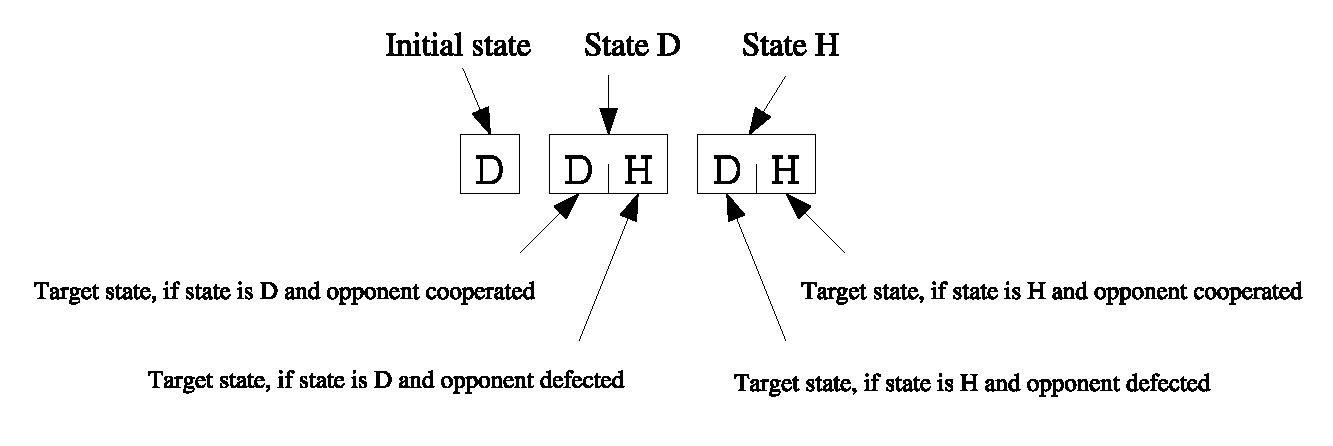
\includegraphics[width=12cm]{images/AutomataRepresentation.eps}
\caption{\label{AutomataRepresentation} Coding players in the repeated
  Prisoner's Dilemma as two state automata. The example shows the
  string representation for the automaton that plays {\em Tit for
    Tat}.}
\end{center}
\end{figure}

Accordingly, two state automata can be implemented by a simple table look-up
algorithm, as can be seen in the following abbreviated code snippet:

\begin{scriptsize}
\begin{verbatim}

class TwoStateAutomaton(Strategy):

    def __init__(self, programString="DDHDH"):
        Strategy.__init__(self)
        self.name = "AM: " + programString

        dic = { 'D':1, 'H':0 }
        self.initialState = dic[programString[0]]
        self.state = self.initialState
        self.progString = programString
        self.prog = [ [dic[programString[4]], dic[programString[3]]], \
                      [dic[programString[2]], dic[programString[1]]] ]

    def firstMove(self):
        self.state = self.initialState
        return self.state

    def nextMove(self, myMoves, opMoves):
        self.state = self.prog[self.state][opMoves[-1]]
        return self.state

\end{verbatim}
\end{scriptsize}

The string representation allows for 32 ($2^5$) different encodings,
but in fact there exist only 26 different automata, because the
automata that represent the strategies {\em Dove} and {\em Hawk} can
be encoded in four different ways (since there are four ($2^2$)
different codings for the state that is never reached). By convenience
we will pick the string representation ``DDDDD'' for the strategy
{\em Dove} and ``HHHHH'' for the strategy {\em Hawk}. Table
\ref{AllTwoStateAutomata} shows all possible two state automata. Some
of them have been given names either to indicate which algorithmic
strategy they represent or just fancy names that where partly taken from
\cite[p. 296]{binmore:1998} (who in turn borrowed them from ``Alice in
Wonderland'').

\begin{figure}
\begin{center}
\begin{tabular}{llll}
1.  & DDDDD (Dove)        & 14. & HDDDD \\
2.  & DDHDD (Tweedledee)  & 15. & HDDDH \\
3.  & DDHDH (Tit for Tat) & 16. & HDDHD (Tweetypie) \\
4.  & DDHHD (Tweedledum)  & 17. & HDHDD (Simpleton) \\
5.  & DDHHH (Grim)        & 18. & HDHDH \\
6.  & DHDDD               & 19. & HDHHD (Pavlov) \\
7.  & DHDDH               & 20. & HHDDD \\
8.  & DHDHD               & 21. & HHDDH \\
9.  & DHDHH               & 22. & HHDHD (Inverted TFT) \\
10. & DHHDD               & 23. & HHHDD \\
11. & DHHDH               & 24. & HHHDH \\
12. & DHHHD               & 25. & HHHHD \\
13. & DHHHH               & 26. & HHHHH \\
\end{tabular}
\caption{\label{AllTwoStateAutomata} List of all possible two state
  automata. The additional names are mostly taken from
  \cite[p. 296]{binmore:1998}.}
\end{center}
\end{figure}


\newpage

\subsection{The family of {\em Signaling Cheater} strategies}
\label{signalingCheaters}

A {\em Singalling Cheater}-strategy is a strategy that plays a predefined
sequence of cooperative and defective moves in the first $n$ rounds of the
repeated Prisoner's Dilemma. If
the opponent player starts with exactly the same sequence of moves, {\em
  Signaling Cheater} assumes that it has met another {\em Signaling Cheater}
and cooperates unconditionally for the remaining rounds of the repeated game.
Otherwise {\em Signaling Cheater} defects for the rest of the game. Thus,
{\em Signaling Cheater} is a strategy that is designed to cooperate only with
its own kind (that is other {\em Signaling Cheaters} that use the same
starting sequence as a signal) and not to cooperate with any other strategy.
The {\tt Python} implementation of {\em Signaling Cheater} follows below:

\begin{scriptsize}
\begin{verbatim}
class SignalingCheater(Strategy):
    def __repr__(self):
        return self.__class__.__name__+"("+repr(self.signal)+")"
    def __init__(self, signal=(0,1,1)):
        Strategy.__init__(self)
        self.signal = signal
        for i in self.signal: self.name += str(i)
    def firstMove(self):
        self.pos = 0
        return self.signal[self.pos]
    def nextMove(self, myMoves, opMoves):
        self.pos += 1
        if self.pos < len(self.signal):
            return self.signal[self.pos]
        else:
            if tuple(opMoves[:len(self.signal)]) == self.signal:
                return 1
            else: return 0
\end{verbatim}
\end{scriptsize}


\newpage

\section{Implementation details of the population dynamics}
\label{implementationDetails}

The population dynamical processes at the base of the simulations in
this book are modeled in a very common and straight forward way: At
the center of most simulations is the evolutionary success of certain
strategies in games such as the repeated Prisoner's Dilemma game. We
assume a population of players where each player plays one of the
strategies. (If this seems to abstract, it may help to think of the
strategies as species and of the players as individuals belonging to
the one or the other species, or to think of the strategies as
mutually exclusive social norms and the players as people that chose
which norm they adhere to.) The players that play a certain strategy
thus constitute the population share of this strategy. For the sake of
simplicity an infinitely large population of players is assumed. The
size of the population share of a strategy is expressed as a fraction
of 1. In the beginning the shares are usually divided equal among all
strategies. The evolutionary process is modeled as a sequence of non
overlapping generational cycles. During each generation the fitness of
every strategy is determined by the average score in the tournament,
where the score of each match is weighted with the population share of
the opponent.  Thus the fitness is determined by:

\begin{equation}
\label{fitnessEquation}
F_i = \sum_{k=1}^n S_{ik}P_k
\end{equation}
\begin{tabular}{lll}
  $F_i$    & &  the Fitness of the $i$-th strategy \\
  $S_{ik}$  & & the score of the $i$-th strategy when playing against
the $k$-th strategy \\
  $P_k$  & & the population share of $k$-th strategy \\
  $n$ & & the total number of strategies in the simulation \\
  $i,k$ & & indices of the strategies \\
& & \\
\end{tabular}

In the simulation program the calculation of the fitness is performed by one
of the different {\tt Fitness} functions in module {\tt Dynamics\-.\-py} of
package {\tt Population\-Dynamics}. The simplemost of these is the function
{\tt Dynamics\-.\-\_Quick\-Fitness2}. If calculates the fitness values of a
population of strategies based on a two player game. The function {\tt
  \_QuickFitness2} is called with the tuple of population shares and the
payoff matrix as parameters. The payoff matrix contains the payoff of the
matches of each strategy against every other strategy. The function returns
the list of fitness values of the strategies.\footnote{This and the following
  code snipplets are taken from module {\tt PopulationDynamics.Dynamics}. For
  the sake of brevity and better readability the error checking code has been
  left out here.}

\begin{scriptsize}
\begin{verbatim}
 1: def _QuickFitness2(population, payoff):
 2:     n = population
 3:     L = len(n)
 4:     p = []
 5:     for i in xrange(L):
 6:         s = 0.0
 7:         for k in xrange(L):
 8:             s += payoff[i,k]*n[k]
 9:         p.append(s)
10:     return p
\end{verbatim}
\end{scriptsize}

The fitness $F_i$ of equation \ref{fitnessEquation} is calculated in
the {\tt for} loop in lines 7 and 8. The outer {\tt for} loop (lines 5
to 9) calculates the fitness for each strategy and appends it to the
list of fitness values. (The assignment in line 2 is done just for
convenience to avoid to many long variable names in line 8.)

One of the parameters that is varied in the simulation series' (see
\ref{refinedModel}) is the parameter {\em e} for the correlation of players of
the same strategy. If {\em e} is nonzero then players with the same strategy
interact more often than with purely random matching. In order to integrate
correlation into the model the original fitness equation
(\ref{fitnessEquation}) must be slightly changed.\footnote{This very simple
  model of correlation was taken from \cite[p. 113, note 30]{skyrms:1996}.}

\begin{equation}
\label{extendedFitnessEquation}
F_i = \sum_{\substack{k = 1 \\ k \ne i}}^n S_{ik}(1-e)P_k + S_{ii}(P_i +
e(1-P_i))
\end{equation}
\begin{tabular}{lll}
  $F_i$    & &  the Fitness of the $i$-th strategy \\
  $S_{ik}$  & & the score of the $i$-th strategy when playing against
the $k$-th strategy \\
  $P_k$  & & the population share of $k$-th strategy \\
  $n$ & & the total number of strategies in the simulation \\
  $i,k$ & & indices of the strategies \\
  $e$ & & the correlation factor, ranging from 0 to 1 \\
& & \\
\end{tabular}

It should be observed that if the correlation $e=0$ then equation
(\ref{extendedFitnessEquation} resolves to the simpler equation
(\ref{fitnessEquation}). But if the correlation $e=1$ (perfect correlation)
then $F_i = S_{ii}$, which is exactly what we would expect: When the
correlation is perfect, players of one strategy never interact with players
of any other strategy and their fitness depends entirely on how the strategy
scores against itself. The implementation of the fitness functions that
includes correlation looks accordingly:

\begin{scriptsize}
\begin{verbatim}
 1: def _Fitness2(population, payoff, e):
 2:     n = population
 3:     L = len(n) 
 4:     p = []    
 5:     for i in xrange(L):
 6:         s = 0.0
 7:         for k in xrange(L):
 8:             if i == k:
 9:                 s += payoff[i,k]*(n[i]+e*(1.0-n[i]))
10:             else: 
11:                 s += payoff[i,k]*(n[k]-e*n[k])
12:         p.append(s)
13:     return p
\end{verbatim}
\end{scriptsize}

The population shares of the next generation are then determined simply by
multiplying the population share of each strategy with its fitness. Since we
calculate with population shares and not with absolute population sizes the
fitness values always express relative fitness. (It makes no difference if
strategy A has a fitness of 1 and strategy B has a fitness of 2 or if A has
fitness 50 and B fitness 100.)  For convenience, the population shares are
normalized (by dividing them through the sum of the not normalized population
shares) so that they nicely add up to 1:

\begin{equation}
\label{populationEquation}
P_i^{g+1} = \frac{P_i^gF_i^g}{\sum_{k=1}^n P_k^gF_k^g}
\end{equation}
\begin{tabular}{lll}
$P_i^g$ & & the population share of strategy $i$ in generation $g$ \\
$F_i^g$ & & the fitness of the $i$-th strategy in generation $g$ \\
$g$ & & the number of the current generation \\
$i,k$ & & indices of the strategies \\
& & \\
\end{tabular} 

The program code that performs these calculations looks as follows:

\begin{scriptsize}
\begin{verbatim}
 1: def _QuickReplicator(population, fitness):
 2:     n = list(population)
 3:     L = len(population)
 4:     f = fitness(population)
 5:     for i in xrange(L): n[i] *= f[i]
 6:     N = sum(n)
 7:     for i in xrange(L): n[i] /= N
 8:     return tuple(n)
\end{verbatim}
\end{scriptsize}

The function {\tt Dynamics\-.\-\_Quick\-Replicator} of package {\tt
  Population\-Dynamics} takes the tuple of population shares and a
fitness function as parameters and returns the tuple of population
shares of the next generation. The fitness function is called in line
4. It is expected to return a list with the fitness values of the
strategies. (As it takes only one parameter the above fitness
function, which takes two parameters, cannot be called directly from
the replicator function, but must be called indirectly through a
dynamically created function that includes the payoff matrix as a
constant parameter. There are technical reasons for using this
construction instead of passing through the payoff matrix from the
caller of the replicator function to the fitness function.) The actual
calculation of the next generation's population shares $P_i^{g+1}$ of
equation \ref{populationEquation} are carried out in lines 5 to 8.

Just as in the case of the fitness equation (\ref{fitnessEquation}) and the
related program code there exists an extended version of the population
equation (\ref{populationEquation}) for the case when the background noise $b
> 0$: 

\begin{equation}
\label{extendedPopulationEquation}
P_i^{g+1} = \frac{P_i^gF_i^g(1-bR_i^g)}{\sum_{k=1}^n P_k^gF_k^g(1-bR_k^g)}
\end{equation}
\begin{tabular}{lll}
$P_i^g$ & & the population share of strategy $i$ in generation $g$ \\
$F_i$ & & the fitness of the $i$-th strategy in generation $g$ \\
$g$ & & the number of the current generation \\
$i,k$ & & indices of the strategies \\
$b$ & & evolutionary background noise $ 0 \le b \le 1$ \\
$R_i^g$ & & a random number $0 \le R_i^g < 1$ \\
& & \\
\end{tabular} 

The implementation in {\tt Python} code is likewise:

\begin{scriptsize}
\begin{verbatim}
 1: def _Replicator(population, fitness, noise):
 2:     n = list(population)
 3:     L = len(population)
 4:     f = fitness
 5:     for i in xrange(L):  n[i] *= f[i]- random.uniform(0,f[i]*noise)
 6:     N = sum(n)
 7:     for i in xrange(L): n[i] /= N
 8:     return tuple(n)
\end{verbatim}
\end{scriptsize}

A few things need to be noted about the model as well as its implementation.
When using infinite populations this is of course an idealization. It makes it
easier to calculate with population shares and, as the model is purely
conceptual and we do not have any particular empirical application of the
model in mind, any fixed finite population size would be arbitrary anyway.
However, the use of infinite populations for modeling processes that take
place in finite populations slightly distorts the evolutionary process in two
ways: 1) Even the slightest variations in fitness lead to variations in
population shares.  In real life, or in nature for that matter, it is
conceivable that very small fitness differences are not strong enough to
transform into a different number of offspring\footnote{It is important here
  that the fitness and the number of offspring are not the same by definition.
  For a short discussion of this point see page \pageref{tautologyCharge}.}
and 2) and more importantly, as long as the fitness value remains above zero,
a species (or strategy respectively) can never die out. Its population share
could be arbitrarily small, yet there is still a possibility that it will
eventually recover, even though in ``real life'' it would never be given a
second chance.  Of course, both of these distortions can, if necessary, easily
be remedied by 1) mapping the fitness onto a discrete set of numbers before
calculating the population shares of the next generation and 2) defining a
threshold population share below which a species (or strategy in our case)
will be eliminated from the population, but it is important to keep these
points in mind.

They way in which the fitness is derived from the payoffs in the
(Prisoner's Dilemma) game also introduces certain peculiarities.
Because the weighted average payoff is used as fitness value, negative
payoffs are impermissible. This may seem awkward given that negative
payoffs are usually perfectly legitimate in game theory and might even
be given a reasonable interpretation, for example, to indicate a loss
of money in an economical context. But if we think of fitness in an
evolutionary context, it makes perfectly good sense to exclude negative
payoffs, because the reproduction rate cannot conceivably fall below
zero. A reproduction rate of zero already means -- depending on the
context -- the extinction of a species, the vanishing of a gene or the
disappearance of a social norm. What worse could happen in evolution
than extinction?

The simulation models described in sections \ref{simpleModel} and
\ref{refinedModel} do even make it impossible that the fitness value
will be exactly zero, because even though some strategies may be left
with a payoff of zero in the repeated Prisoner's Dilemma match against
another strategy (as, for example, {\em Dove} against {\em Hawk}) the
average payoff of a strategy in the tournament can never be zero,
because no strategy gets a zero payoff in the match against itself.
This simplifies calculations greatly, because no provisions for the
special case of a zero fitness need to be made. Otherwise, care would
have to be taken to avoid divisions by zero and the like.

\newpage
\section{Comprehensive results of the simualtion series}
\label{completeTables}

The following tables and figures list all of aggregated data of the simulation
series described in chapter \ref{refinedModel}. First (section
\ref{BigSeriesResults}) the overall results of the big series are given, both
as tables and then in a graphical form. The stratgey set of {\em Two State
Automata} (section \ref{twoStateAutomata} above) and the set of {\em
Parameterized Tit for Tats} (section \ref{parameterizedTFTs}) are always
considered separately. In the tables the the average final population shares
of the evolutionary simulations is displayed. (The simulations in the series
were stopped either when no changes in the composition of the population
occured any more or when the 25,600th generation had been reached.) The
strategies are always ranked after their average final population share in the
whole series. The graphical representation depicts in three columns the
tournament ranking (in lexical order that is, if a strategy has been the the
winner of the tournament two times over the whole series it is always better
than a strategy that has won the tournament only once, no matter how often it
was placed second), the evolutionary ranking (by the average final population
share) and a more illustrative representation of the evolutionary ranking. On
the graphical representation, the strategies are represented by colored bars,
which represent their degree of altruism. A green color means that the strategy
is fully (e.g. {\em Dove}) or to some degree (e.g. {\em Tweedledee}) genuinely
altruistic. A blue color means that it is either reciprocal (e.g. {\em Tit for
Tat}, {\em Grim}) or cannot be classified (e.g. {\em Inverted}). Red means that
the strategy is a cheater or (primarily) non altruistic (e.g. {\em Hawk}). (See
page \pageref{colorScheme} for detailed description of the color scheme and its
motivation.)

In order to determine the influence of single parameters on the simulation, the
aggregated results for every parameter held constant at each of its values (see
page \pageref{seriesParameters}) was calculated as well. This helps to
find out about the influence of single parameters on the simulation, though
possible joint effects of several parameters still remain opaque. For each
parameter and strategy set, a table is presented that shows how the average
final population share of each strategy changes for different values of the
parameter. There is also a graphical representation of the tournament rankings
and evolutionary outcomes for each parameter value and strategy set.

\newpage
\subsection{``Big series'' overall results}
\label{BigSeriesResults}

\begin{tabular}{|l|r|}
\hline
 & \multicolumn{1}{c|}{{\bf Average Final Population Share}} \\
\hline
{\bf Strategy} & overall results\\ \hline
AM: HHHHH (HAWK)             &   34.61 \% \\
AM: DDHHH (GRIM)             &   17.28 \% \\
AM: DDHDH (TIT FOR TAT)      &   10.22 \% \\
AM: HDHHD (PAVLOV)           &   10.01 \% \\
AM: DDDDD (DOVE)             &    9.27 \% \\
AM: DDHHD (TWEEDLEDUM)       &    7.12 \% \\
AM: DDHDD (TWEEDLEDEE)       &    2.91 \% \\
AM: HDHDH (TAT FOR TIT)      &    1.73 \% \\
AM: DHHHH                    &    1.56 \% \\
AM: DHHDH                    &    1.39 \% \\
AM: HDHDD (SIMPLETON)        &    1.28 \% \\
AM: HHHDH                    &    1.09 \% \\
AM: HHHHD                    &    0.52 \% \\
AM: DHHDD                    &    0.39 \% \\
AM: HHHDD                    &    0.36 \% \\
AM: DHHHD                    &    0.13 \% \\
AM: DHDHH                    &    0.10 \% \\
AM: HDDHD (TWEETYPIE)        &    0.00 \% \\
AM: HHDHD (INVERTED)         &    0.00 \% \\
AM: DHDHD                    &    0.00 \% \\
AM: HDDDD                    &    0.00 \% \\
AM: HHDDD                    &    0.00 \% \\
AM: DHDDD                    &    0.00 \% \\
AM: HDDDH                    &    0.00 \% \\
AM: HHDDH                    &    0.00 \% \\
AM: DHDDH                    &    0.00 \% \\
\hline
\end{tabular}


\newpage
\begin{tabular}{|l|r|}
\hline
 & \multicolumn{1}{c|}{{\bf Average Final Population Share}} \\
\hline
{\bf Strategy} & overall results\\ \hline
P\_TFT 0.00 0.00 (TitForTat)  &   38.54 \% \\
P\_TFT 0.00 1.00 (Hawk)       &   28.50 \% \\
P\_TFT 0.20 0.00              &    8.98 \% \\
P\_TFT 1.00 0.00 (Dove)       &    8.30 \% \\
P\_TFT 0.40 0.00              &    8.27 \% \\
P\_TFT 0.80 0.00              &    2.16 \% \\
P\_TFT 1.00 1.00 (Inverted)   &    1.55 \% \\
P\_TFT 0.00 0.80              &    1.06 \% \\
P\_TFT 0.20 0.40              &    0.93 \% \\
P\_TFT 0.60 0.00              &    0.51 \% \\
P\_TFT 0.40 0.20              &    0.46 \% \\
P\_TFT 0.60 1.00              &    0.38 \% \\
P\_TFT 0.40 0.40              &    0.23 \% \\
P\_TFT 0.60 0.20              &    0.12 \% \\
P\_TFT 0.80 1.00              &    0.01 \% \\
P\_TFT 0.40 1.00              &    0.00 \% \\
P\_TFT 0.20 1.00              &    0.00 \% \\
P\_TFT 0.00 0.60              &    0.00 \% \\
P\_TFT 0.80 0.20              &    0.00 \% \\
P\_TFT 1.00 0.20              &    0.00 \% \\
P\_TFT 0.80 0.40              &    0.00 \% \\
P\_TFT 0.20 0.20              &    0.00 \% \\
P\_TFT 0.60 0.40              &    0.00 \% \\
P\_TFT 1.00 0.40              &    0.00 \% \\
P\_TFT 0.00 0.40              &    0.00 \% \\
P\_TFT 0.80 0.60              &    0.00 \% \\
P\_TFT 1.00 0.60              &    0.00 \% \\
P\_TFT 0.00 0.20              &    0.00 \% \\
P\_TFT 0.60 0.60              &    0.00 \% \\
P\_TFT 0.40 0.60              &    0.00 \% \\
P\_TFT 0.20 0.60              &    0.00 \% \\
P\_TFT 0.80 0.80              &    0.00 \% \\
P\_TFT 0.20 0.80              &    0.00 \% \\
P\_TFT 0.60 0.80              &    0.00 \% \\
P\_TFT 0.40 0.80              &    0.00 \% \\
P\_TFT 1.00 0.80              &    0.00 \% \\
\hline
\end{tabular}


\begin{sidewaysfigure}
\begin{center}
\includegraphics[width=20cm]{tables/Automata_overall.eps}
\caption{\label{Automata_Overall} The aggregated results of all simulations
of the ``big series'' using {\em Automata} strategies.}
\end{center}
\end{sidewaysfigure}

\begin{sidewaysfigure}
\begin{center}
\includegraphics[width=20cm]{tables/TFTs_overall.eps}
\caption{\label{TFTs_Overall} The aggregated results of all simulations
of the ``big series'' using {\em Parameterized Tit for Tat} strategies.}
\end{center}
\end{sidewaysfigure}


\newpage
\subsection{The influence of correlation}

The correlation factor describes the probability by which players are
more likely to meet opponents with the same strategy than opponents with a
different strategy. A correlation of 0\% means that the players are randomly
matched, while with a correlation of 100\% players do exclusively play
against players of the same strategy.

\subsubsection{Automata}
\begin{tabular}{|l|r|r|r|r|}
\hline
 & \multicolumn{4}{c|}{{\bf Average Final Population Share}} \\
\hline
{\bf Strategy} & overall &  c = 0.0 & c = 0.1 & c = 0.2\\ \hline
AM: HHHHH (HAWK)             &   34.61 \%  &   44.30 \%  &   33.71 \%  &   25.81 \% \\
AM: DDHHH (GRIM)             &   17.28 \%  &   21.73 \%  &   16.27 \%  &   13.85 \% \\
AM: DDHDH (TIT FOR TAT)      &   10.22 \%  &    9.51 \%  &   13.47 \%  &    7.69 \% \\
AM: HDHHD (PAVLOV)           &   10.01 \%  &    2.08 \%  &    4.83 \%  &   23.11 \% \\
AM: DDDDD (DOVE)             &    9.27 \%  &    8.04 \%  &   11.29 \%  &    8.48 \% \\
AM: DDHHD (TWEEDLEDUM)       &    7.12 \%  &    2.58 \%  &    4.95 \%  &   13.82 \% \\
AM: DDHDD (TWEEDLEDEE)       &    2.91 \%  &    2.70 \%  &    4.40 \%  &    1.63 \% \\
AM: HDHDH (TAT FOR TIT)      &    1.73 \%  &    0.00 \%  &    1.88 \%  &    3.32 \% \\
AM: DHHHH                    &    1.56 \%  &    4.69 \%  &    0.00 \%  &    0.00 \% \\
AM: DHHDH                    &    1.39 \%  &    0.53 \%  &    2.62 \%  &    1.02 \% \\
AM: HDHDD (SIMPLETON)        &    1.28 \%  &    0.62 \%  &    2.57 \%  &    0.66 \% \\
AM: HHHDH                    &    1.09 \%  &    0.56 \%  &    2.11 \%  &    0.61 \% \\
AM: HHHHD                    &    0.52 \%  &    0.78 \%  &    0.79 \%  &    0.00 \% \\
AM: DHHDD                    &    0.39 \%  &    0.86 \%  &    0.32 \%  &    0.00 \% \\
AM: HHHDD                    &    0.36 \%  &    0.70 \%  &    0.39 \%  &    0.00 \% \\
AM: DHHHD                    &    0.13 \%  &    0.00 \%  &    0.40 \%  &    0.00 \% \\
AM: DHDHH                    &    0.10 \%  &    0.29 \%  &    0.00 \%  &    0.00 \% \\
AM: HDDHD (TWEETYPIE)        &    0.00 \%  &    0.00 \%  &    0.00 \%  &    0.00 \% \\
AM: HHDHD (INVERTED)         &    0.00 \%  &    0.00 \%  &    0.00 \%  &    0.00 \% \\
AM: DHDHD                    &    0.00 \%  &    0.00 \%  &    0.00 \%  &    0.00 \% \\
AM: HDDDD                    &    0.00 \%  &    0.00 \%  &    0.00 \%  &    0.00 \% \\
AM: HHDDD                    &    0.00 \%  &    0.00 \%  &    0.00 \%  &    0.00 \% \\
AM: DHDDD                    &    0.00 \%  &    0.00 \%  &    0.00 \%  &    0.00 \% \\
AM: HDDDH                    &    0.00 \%  &    0.00 \%  &    0.00 \%  &    0.00 \% \\
AM: HHDDH                    &    0.00 \%  &    0.00 \%  &    0.00 \%  &    0.00 \% \\
AM: DHDDH                    &    0.00 \%  &    0.00 \%  &    0.00 \%  &    0.00 \% \\
\hline
\end{tabular}


\begin{sidewaysfigure}
\begin{center}
\includegraphics[width=20cm]{tables/Automata_C0.000.eps}
\caption{\label{Automata_C0000} The aggregated results of those
simulations of the ``big series'' for which the correlation value was 0\%.}
\end{center}
\end{sidewaysfigure}

\begin{sidewaysfigure}
\begin{center}
\includegraphics[width=20cm]{tables/Automata_C0.100.eps}
\caption{\label{Automata_C0100} The aggregated results of those
simulations of the ``big series'' for which the correlation value was 10\%.}
\end{center}
\end{sidewaysfigure}

\begin{sidewaysfigure}
\begin{center}
\includegraphics[width=20cm]{tables/Automata_C0.200.eps}
\caption{\label{Automata_C0200} The aggregated results of those
simulations of the ``big series'' for which the correlation value was 20\%.}
\end{center}
\end{sidewaysfigure}

\newpage
\subsubsection{Parameterized Tit for Tats}
\begin{tabular}{|l|r|r|r|r|}
\hline
 & \multicolumn{4}{c|}{{\bf Average Final Population Share}} \\
\hline
{\bf Strategy} & overall &  c = 0.0 & c = 0.1 & c = 0.2\\ \hline
P\_TFT 0.00 0.00 (TitForTat)  &   38.54 \%  &   32.71 \%  &   42.20 \%  &   40.72 \% \\
P\_TFT 0.00 1.00 (Hawk)       &   28.50 \%  &   54.45 \%  &   25.76 \%  &    5.29 \% \\
P\_TFT 0.20 0.00              &    8.98 \%  &    0.87 \%  &    6.84 \%  &   19.22 \% \\
P\_TFT 1.00 0.00 (Dove)       &    8.30 \%  &    1.27 \%  &    7.15 \%  &   16.49 \% \\
P\_TFT 0.40 0.00              &    8.27 \%  &    4.14 \%  &    9.60 \%  &   11.06 \% \\
P\_TFT 0.80 0.00              &    2.16 \%  &    0.70 \%  &    2.11 \%  &    3.68 \% \\
P\_TFT 1.00 1.00 (Inverted)   &    1.55 \%  &    1.24 \%  &    1.54 \%  &    1.88 \% \\
P\_TFT 0.00 0.80              &    1.06 \%  &    1.80 \%  &    1.37 \%  &    0.00 \% \\
P\_TFT 0.20 0.40              &    0.93 \%  &    2.78 \%  &    0.00 \%  &    0.00 \% \\
P\_TFT 0.60 0.00              &    0.51 \%  &    0.05 \%  &    0.78 \%  &    0.70 \% \\
P\_TFT 0.40 0.20              &    0.46 \%  &    0.00 \%  &    1.39 \%  &    0.00 \% \\
P\_TFT 0.60 1.00              &    0.38 \%  &    0.00 \%  &    0.37 \%  &    0.78 \% \\
P\_TFT 0.40 0.40              &    0.23 \%  &    0.00 \%  &    0.69 \%  &    0.00 \% \\
P\_TFT 0.60 0.20              &    0.12 \%  &    0.00 \%  &    0.19 \%  &    0.17 \% \\
P\_TFT 0.80 1.00              &    0.01 \%  &    0.00 \%  &    0.02 \%  &    0.01 \% \\
P\_TFT 0.40 1.00              &    0.00 \%  &    0.00 \%  &    0.00 \%  &    0.00 \% \\
P\_TFT 0.20 1.00              &    0.00 \%  &    0.00 \%  &    0.00 \%  &    0.00 \% \\
P\_TFT 0.00 0.60              &    0.00 \%  &    0.00 \%  &    0.00 \%  &    0.00 \% \\
P\_TFT 0.80 0.20              &    0.00 \%  &    0.00 \%  &    0.00 \%  &    0.00 \% \\
P\_TFT 1.00 0.20              &    0.00 \%  &    0.00 \%  &    0.00 \%  &    0.00 \% \\
P\_TFT 0.80 0.40              &    0.00 \%  &    0.00 \%  &    0.00 \%  &    0.00 \% \\
P\_TFT 0.20 0.20              &    0.00 \%  &    0.00 \%  &    0.00 \%  &    0.00 \% \\
P\_TFT 0.60 0.40              &    0.00 \%  &    0.00 \%  &    0.00 \%  &    0.00 \% \\
P\_TFT 1.00 0.40              &    0.00 \%  &    0.00 \%  &    0.00 \%  &    0.00 \% \\
P\_TFT 0.00 0.40              &    0.00 \%  &    0.00 \%  &    0.00 \%  &    0.00 \% \\
P\_TFT 0.80 0.60              &    0.00 \%  &    0.00 \%  &    0.00 \%  &    0.00 \% \\
P\_TFT 1.00 0.60              &    0.00 \%  &    0.00 \%  &    0.00 \%  &    0.00 \% \\
P\_TFT 0.00 0.20              &    0.00 \%  &    0.00 \%  &    0.00 \%  &    0.00 \% \\
P\_TFT 0.60 0.60              &    0.00 \%  &    0.00 \%  &    0.00 \%  &    0.00 \% \\
P\_TFT 0.40 0.60              &    0.00 \%  &    0.00 \%  &    0.00 \%  &    0.00 \% \\
P\_TFT 0.20 0.60              &    0.00 \%  &    0.00 \%  &    0.00 \%  &    0.00 \% \\
P\_TFT 0.80 0.80              &    0.00 \%  &    0.00 \%  &    0.00 \%  &    0.00 \% \\
P\_TFT 0.20 0.80              &    0.00 \%  &    0.00 \%  &    0.00 \%  &    0.00 \% \\
P\_TFT 0.60 0.80              &    0.00 \%  &    0.00 \%  &    0.00 \%  &    0.00 \% \\
P\_TFT 0.40 0.80              &    0.00 \%  &    0.00 \%  &    0.00 \%  &    0.00 \% \\
P\_TFT 1.00 0.80              &    0.00 \%  &    0.00 \%  &    0.00 \%  &    0.00 \% \\
\hline
\end{tabular}


\begin{sidewaysfigure}
\begin{center}
\includegraphics[width=20cm]{tables/TFTs_C0.000.eps}
\caption{\label{TFTs_C0000} The aggregated results of those
simulations of the ``big series'' for which the correlation value was 0\%.}
\end{center}
\end{sidewaysfigure}

\begin{sidewaysfigure}
\begin{center}
\includegraphics[width=20cm]{tables/TFTs_C0.100.eps}
\caption{\label{TFTs_C0100} The aggregated results of those
simulations of the ``big series'' for which the correlation value was 10\%.}
\end{center}
\end{sidewaysfigure}

\begin{sidewaysfigure}
\begin{center}
\includegraphics[width=20cm]{tables/TFTs_C0.200.eps}
\caption{\label{TFTs_C0200} The aggregated results of those
simulations of the ``big series'' for which the correlation value was 20\%.}
\end{center}
\end{sidewaysfigure}


\newpage
\subsection{The influence of game noise}

The game noise parameter specifies a probability with which the
intended move of a player is randomly turned into its opposite.

\subsubsection{Automata}
\begin{tabular}{|l|r|r|r|r|}
\hline
 & \multicolumn{4}{c|}{{\bf Average Final Population Share}} \\
\hline
{\bf Strategy} & overall &  g = 0.0 & g = 0.05 & g = 0.1\\ \hline
AM: HHHHH (HAWK)             &   34.61 \%  &    7.45 \%  &   36.38 \%  &   59.99 \% \\
AM: DDHHH (GRIM)             &   17.28 \%  &   38.23 \%  &   10.42 \%  &    3.19 \% \\
AM: DDHDH (TIT FOR TAT)      &   10.22 \%  &   15.82 \%  &    7.78 \%  &    7.07 \% \\
AM: HDHHD (PAVLOV)           &   10.01 \%  &    5.03 \%  &   16.48 \%  &    8.51 \% \\
AM: DDDDD (DOVE)             &    9.27 \%  &   22.58 \%  &    3.67 \%  &    1.56 \% \\
AM: DDHHD (TWEEDLEDUM)       &    7.12 \%  &    7.08 \%  &    9.13 \%  &    5.14 \% \\
AM: DDHDD (TWEEDLEDEE)       &    2.91 \%  &    3.81 \%  &    4.66 \%  &    0.26 \% \\
AM: HDHDH (TAT FOR TIT)      &    1.73 \%  &    0.00 \%  &    2.57 \%  &    2.64 \% \\
AM: DHHHH                    &    1.56 \%  &    0.00 \%  &    0.74 \%  &    3.95 \% \\
AM: DHHDH                    &    1.39 \%  &    0.00 \%  &    1.72 \%  &    2.45 \% \\
AM: HDHDD (SIMPLETON)        &    1.28 \%  &    0.00 \%  &    0.93 \%  &    2.92 \% \\
AM: HHHDH                    &    1.09 \%  &    0.00 \%  &    2.02 \%  &    1.26 \% \\
AM: HHHHD                    &    0.52 \%  &    0.00 \%  &    1.46 \%  &    0.12 \% \\
AM: DHHDD                    &    0.39 \%  &    0.00 \%  &    1.01 \%  &    0.17 \% \\
AM: HHHDD                    &    0.36 \%  &    0.00 \%  &    0.86 \%  &    0.23 \% \\
AM: DHHHD                    &    0.13 \%  &    0.00 \%  &    0.16 \%  &    0.24 \% \\
AM: DHDHH                    &    0.10 \%  &    0.00 \%  &    0.00 \%  &    0.29 \% \\
AM: HDDHD (TWEETYPIE)        &    0.00 \%  &    0.00 \%  &    0.00 \%  &    0.00 \% \\
AM: HHDHD (INVERTED)         &    0.00 \%  &    0.00 \%  &    0.00 \%  &    0.00 \% \\
AM: DHDHD                    &    0.00 \%  &    0.00 \%  &    0.00 \%  &    0.00 \% \\
AM: HDDDD                    &    0.00 \%  &    0.00 \%  &    0.00 \%  &    0.00 \% \\
AM: HHDDD                    &    0.00 \%  &    0.00 \%  &    0.00 \%  &    0.00 \% \\
AM: DHDDD                    &    0.00 \%  &    0.00 \%  &    0.00 \%  &    0.00 \% \\
AM: HDDDH                    &    0.00 \%  &    0.00 \%  &    0.00 \%  &    0.00 \% \\
AM: HHDDH                    &    0.00 \%  &    0.00 \%  &    0.00 \%  &    0.00 \% \\
AM: DHDDH                    &    0.00 \%  &    0.00 \%  &    0.00 \%  &    0.00 \% \\
\hline
\end{tabular}


\begin{sidewaysfigure}
\begin{center}
\includegraphics[width=20cm]{tables/Automata_G0.000.eps}
\caption{\label{Automata_G0000} The aggregated results of those
simulations of the ``big series'' for which the game noise was 0\%.}
\end{center}
\end{sidewaysfigure}

\begin{sidewaysfigure}
\begin{center}
\includegraphics[width=20cm]{tables/Automata_G0.050.eps}
\caption{\label{Automata_G0050} The aggregated results of those
simulations of the ``big series'' for which the game noise was 5\%.}
\end{center}
\end{sidewaysfigure}

\begin{sidewaysfigure}
\begin{center}
\includegraphics[width=20cm]{tables/Automata_G0.100.eps}
\caption{\label{Automata_G0100} The aggregated results of those
simulations of the ``big series'' for which the game noise was 10\%.}
\end{center}
\end{sidewaysfigure}

\newpage
\subsubsection{Parameterized Tit for Tats}
\begin{tabular}{|l|r|r|r|r|}
\hline
 & \multicolumn{4}{c|}{{\bf Average Final Population Share}} \\
\hline
{\bf Strategy} & overall &  g = 0.0 & g = 0.05 & g = 0.1\\ \hline
P\_TFT 0.00 0.00 (TitForTat)  &   38.54 \%  &   82.41 \%  &   18.98 \%  &   14.24 \% \\
P\_TFT 0.00 1.00 (Hawk)       &   28.50 \%  &    0.00 \%  &   27.39 \%  &   58.11 \% \\
P\_TFT 0.20 0.00              &    8.98 \%  &    6.84 \%  &    8.60 \%  &   11.48 \% \\
P\_TFT 1.00 0.00 (Dove)       &    8.30 \%  &    6.56 \%  &   11.80 \%  &    6.56 \% \\
P\_TFT 0.40 0.00              &    8.27 \%  &    2.60 \%  &   18.94 \%  &    3.25 \% \\
P\_TFT 0.80 0.00              &    2.16 \%  &    0.93 \%  &    4.17 \%  &    1.39 \% \\
P\_TFT 1.00 1.00 (Inverted)   &    1.55 \%  &    0.00 \%  &    3.00 \%  &    1.66 \% \\
P\_TFT 0.00 0.80              &    1.06 \%  &    0.00 \%  &    3.17 \%  &    0.00 \% \\
P\_TFT 0.20 0.40              &    0.93 \%  &    0.00 \%  &    2.78 \%  &    0.00 \% \\
P\_TFT 0.60 0.00              &    0.51 \%  &    0.65 \%  &    0.00 \%  &    0.87 \% \\
P\_TFT 0.40 0.20              &    0.46 \%  &    0.00 \%  &    0.00 \%  &    1.39 \% \\
P\_TFT 0.60 1.00              &    0.38 \%  &    0.00 \%  &    0.13 \%  &    1.02 \% \\
P\_TFT 0.40 0.40              &    0.23 \%  &    0.00 \%  &    0.69 \%  &    0.00 \% \\
P\_TFT 0.60 0.20              &    0.12 \%  &    0.00 \%  &    0.36 \%  &    0.00 \% \\
P\_TFT 0.80 1.00              &    0.01 \%  &    0.00 \%  &    0.00 \%  &    0.03 \% \\
P\_TFT 0.40 1.00              &    0.00 \%  &    0.00 \%  &    0.00 \%  &    0.00 \% \\
P\_TFT 0.20 1.00              &    0.00 \%  &    0.00 \%  &    0.00 \%  &    0.00 \% \\
P\_TFT 0.00 0.60              &    0.00 \%  &    0.00 \%  &    0.00 \%  &    0.00 \% \\
P\_TFT 0.80 0.20              &    0.00 \%  &    0.00 \%  &    0.00 \%  &    0.00 \% \\
P\_TFT 1.00 0.20              &    0.00 \%  &    0.00 \%  &    0.00 \%  &    0.00 \% \\
P\_TFT 0.80 0.40              &    0.00 \%  &    0.00 \%  &    0.00 \%  &    0.00 \% \\
P\_TFT 0.20 0.20              &    0.00 \%  &    0.00 \%  &    0.00 \%  &    0.00 \% \\
P\_TFT 0.60 0.40              &    0.00 \%  &    0.00 \%  &    0.00 \%  &    0.00 \% \\
P\_TFT 1.00 0.40              &    0.00 \%  &    0.00 \%  &    0.00 \%  &    0.00 \% \\
P\_TFT 0.00 0.40              &    0.00 \%  &    0.00 \%  &    0.00 \%  &    0.00 \% \\
P\_TFT 0.80 0.60              &    0.00 \%  &    0.00 \%  &    0.00 \%  &    0.00 \% \\
P\_TFT 1.00 0.60              &    0.00 \%  &    0.00 \%  &    0.00 \%  &    0.00 \% \\
P\_TFT 0.00 0.20              &    0.00 \%  &    0.00 \%  &    0.00 \%  &    0.00 \% \\
P\_TFT 0.60 0.60              &    0.00 \%  &    0.00 \%  &    0.00 \%  &    0.00 \% \\
P\_TFT 0.40 0.60              &    0.00 \%  &    0.00 \%  &    0.00 \%  &    0.00 \% \\
P\_TFT 0.20 0.60              &    0.00 \%  &    0.00 \%  &    0.00 \%  &    0.00 \% \\
P\_TFT 0.80 0.80              &    0.00 \%  &    0.00 \%  &    0.00 \%  &    0.00 \% \\
P\_TFT 0.20 0.80              &    0.00 \%  &    0.00 \%  &    0.00 \%  &    0.00 \% \\
P\_TFT 0.60 0.80              &    0.00 \%  &    0.00 \%  &    0.00 \%  &    0.00 \% \\
P\_TFT 0.40 0.80              &    0.00 \%  &    0.00 \%  &    0.00 \%  &    0.00 \% \\
P\_TFT 1.00 0.80              &    0.00 \%  &    0.00 \%  &    0.00 \%  &    0.00 \% \\
\hline
\end{tabular}


\begin{sidewaysfigure}
\begin{center}
\includegraphics[width=20cm]{tables/TFTs_G0.000.eps}
\caption{\label{TFTs_G0000} The aggregated results of those
simulations of the ``big series'' for which the game noise was 0\%.}
\end{center}
\end{sidewaysfigure}

\begin{sidewaysfigure}
\begin{center}
\includegraphics[width=20cm]{tables/TFTs_G0.050.eps}
\caption{\label{TFTs_G0050} The aggregated results of those
simulations of the ``big series'' for which the game noise was 5\%.}
\end{center}
\end{sidewaysfigure}

\begin{sidewaysfigure}
\begin{center}
\includegraphics[width=20cm]{tables/TFTs_G0.100.eps}
\caption{\label{TFTs_G0100} The aggregated results of those
simulations of the ``big series'' for which the game noise was 10\%.}
\end{center}
\end{sidewaysfigure}


\newpage
\subsection{The influence of evolutionary noise}

Evolutionary noise is here understood as a
random distortion of a certain percentage that will decrease or increase the
fitness value of each strategy in the population dynamics.

\subsubsection{Automata}
\begin{small}
\begin{tabular}{|l|r|r|r|r|r|}
\hline
 & \multicolumn{5}{c|}{{\bf Average Final Population Share}} \\
\hline
{\bf Strategy} & overall &  n = 0.0 & n = 0.05 & n = 0.1 & n = 0.15\\ \hline
AM: HHHHH (HAWK)             &   34.61 \%  &   32.80 \%  &   33.92 \%  &   35.58 \%  &   36.13 \% \\
AM: DDHHH (GRIM)             &   17.28 \%  &   20.28 \%  &   16.40 \%  &   16.29 \%  &   16.16 \% \\
AM: DDHDH (TIT FOR TAT)      &   10.22 \%  &    9.69 \%  &   10.59 \%  &    9.77 \%  &   10.84 \% \\
AM: HDHHD (PAVLOV)           &   10.01 \%  &   10.84 \%  &   10.56 \%  &    9.01 \%  &    9.61 \% \\
AM: DDDDD (DOVE)             &    9.27 \%  &    9.19 \%  &    9.98 \%  &    9.85 \%  &    8.07 \% \\
AM: DDHHD (TWEEDLEDUM)       &    7.12 \%  &    6.45 \%  &    6.22 \%  &   10.10 \%  &    5.69 \% \\
AM: DDHDD (TWEEDLEDEE)       &    2.91 \%  &    2.70 \%  &    3.61 \%  &    2.45 \%  &    2.89 \% \\
AM: HDHDH (TAT FOR TIT)      &    1.73 \%  &    1.25 \%  &    1.14 \%  &    1.56 \%  &    3.00 \% \\
AM: DHHHH                    &    1.56 \%  &    1.47 \%  &    2.10 \%  &    1.08 \%  &    1.61 \% \\
AM: DHHDH                    &    1.39 \%  &    1.34 \%  &    1.24 \%  &    1.26 \%  &    1.72 \% \\
AM: HDHDD (SIMPLETON)        &    1.28 \%  &    1.30 \%  &    1.37 \%  &    1.00 \%  &    1.46 \% \\
AM: HHHDH                    &    1.09 \%  &    1.37 \%  &    0.93 \%  &    0.69 \%  &    1.39 \% \\
AM: HHHHD                    &    0.52 \%  &    0.07 \%  &    0.99 \%  &    0.05 \%  &    0.99 \% \\
AM: DHHDD                    &    0.39 \%  &    0.57 \%  &    0.32 \%  &    0.44 \%  &    0.24 \% \\
AM: HHHDD                    &    0.36 \%  &    0.41 \%  &    0.25 \%  &    0.63 \%  &    0.17 \% \\
AM: DHHHD                    &    0.13 \%  &    0.20 \%  &    0.13 \%  &    0.18 \%  &    0.02 \% \\
AM: DHDHH                    &    0.10 \%  &    0.06 \%  &    0.24 \%  &    0.07 \%  &    0.01 \% \\
AM: HDDHD (TWEETYPIE)        &    0.00 \%  &    0.00 \%  &    0.00 \%  &    0.00 \%  &    0.00 \% \\
AM: HHDHD (INVERTED)         &    0.00 \%  &    0.00 \%  &    0.00 \%  &    0.00 \%  &    0.00 \% \\
AM: DHDHD                    &    0.00 \%  &    0.00 \%  &    0.00 \%  &    0.00 \%  &    0.00 \% \\
AM: HDDDD                    &    0.00 \%  &    0.00 \%  &    0.00 \%  &    0.00 \%  &    0.00 \% \\
AM: HHDDD                    &    0.00 \%  &    0.00 \%  &    0.00 \%  &    0.00 \%  &    0.00 \% \\
AM: DHDDD                    &    0.00 \%  &    0.00 \%  &    0.00 \%  &    0.00 \%  &    0.00 \% \\
AM: HDDDH                    &    0.00 \%  &    0.00 \%  &    0.00 \%  &    0.00 \%  &    0.00 \% \\
AM: HHDDH                    &    0.00 \%  &    0.00 \%  &    0.00 \%  &    0.00 \%  &    0.00 \% \\
AM: DHDDH                    &    0.00 \%  &    0.00 \%  &    0.00 \%  &    0.00 \%  &    0.00 \% \\
\hline
\end{tabular}

\end{small}

\begin{sidewaysfigure}
\begin{center}
\includegraphics[width=20cm]{tables/Automata_N0.000.eps}
\caption{\label{Automata_N0000} The aggregated results of those
simulations of the ``big series'' for which the evolutionary noise was 0\%.}
\end{center}
\end{sidewaysfigure}

\begin{sidewaysfigure}
\begin{center}
\includegraphics[width=20cm]{tables/Automata_N0.050.eps}
\caption{\label{Automata_N0050} The aggregated results of those
simulations of the ``big series'' for which the evolutionary noise was 5\%.}
\end{center}
\end{sidewaysfigure}

\begin{sidewaysfigure}
\begin{center}
\includegraphics[width=20cm]{tables/Automata_N0.100.eps}
\caption{\label{Automata_N0100} The aggregated results of those
simulations of the ``big series'' for which the evolutionary noise was 10\%.}
\end{center}
\end{sidewaysfigure}

\begin{sidewaysfigure}
\begin{center}
\includegraphics[width=20cm]{tables/Automata_N0.150.eps}
\caption{\label{Automata_N0150} The aggregated results of those
simulations of the ``big series'' for which the evolutionary noise was 15\%.}
\end{center}
\end{sidewaysfigure}


\newpage
\subsubsection{Parameterized Tit for Tats}
\begin{small}
\begin{tabular}{|l|r|r|r|r|r|}
\hline
 & \multicolumn{5}{c|}{{\bf Average Final Population Share}} \\
\hline
{\bf Strategy} & overall &  n = 0.0 & n = 0.05 & n = 0.1 & n = 0.15\\ \hline
P\_TFT 0.00 0.00 (TitForTat)  &   38.54 \%  &   41.98 \%  &   38.40 \%  &   35.63 \%  &   38.17 \% \\
P\_TFT 0.00 1.00 (Hawk)       &   28.50 \%  &   26.85 \%  &   28.63 \%  &   29.38 \%  &   29.14 \% \\
P\_TFT 0.20 0.00              &    8.98 \%  &    9.04 \%  &   10.12 \%  &    7.12 \%  &    9.62 \% \\
P\_TFT 1.00 0.00 (Dove)       &    8.30 \%  &    6.09 \%  &    7.59 \%  &   11.21 \%  &    8.31 \% \\
P\_TFT 0.40 0.00              &    8.27 \%  &    8.30 \%  &    7.71 \%  &    7.79 \%  &    9.26 \% \\
P\_TFT 0.80 0.00              &    2.16 \%  &    1.94 \%  &    1.96 \%  &    2.78 \%  &    1.97 \% \\
P\_TFT 1.00 1.00 (Inverted)   &    1.55 \%  &    1.82 \%  &    1.57 \%  &    2.17 \%  &    0.66 \% \\
P\_TFT 0.00 0.80              &    1.06 \%  &    1.02 \%  &    1.03 \%  &    1.27 \%  &    0.91 \% \\
P\_TFT 0.20 0.40              &    0.93 \%  &    0.93 \%  &    0.93 \%  &    0.93 \%  &    0.93 \% \\
P\_TFT 0.60 0.00              &    0.51 \%  &    0.41 \%  &    0.67 \%  &    0.28 \%  &    0.68 \% \\
P\_TFT 0.40 0.20              &    0.46 \%  &    0.00 \%  &    0.93 \%  &    0.93 \%  &    0.00 \% \\
P\_TFT 0.60 1.00              &    0.38 \%  &    0.48 \%  &    0.26 \%  &    0.42 \%  &    0.37 \% \\
P\_TFT 0.40 0.40              &    0.23 \%  &    0.93 \%  &    0.00 \%  &    0.00 \%  &    0.00 \% \\
P\_TFT 0.60 0.20              &    0.12 \%  &    0.19 \%  &    0.21 \%  &    0.08 \%  &    0.00 \% \\
P\_TFT 0.80 1.00              &    0.01 \%  &    0.02 \%  &    0.01 \%  &    0.01 \%  &    0.00 \% \\
P\_TFT 0.40 1.00              &    0.00 \%  &    0.00 \%  &    0.00 \%  &    0.00 \%  &    0.00 \% \\
P\_TFT 0.20 1.00              &    0.00 \%  &    0.00 \%  &    0.00 \%  &    0.00 \%  &    0.00 \% \\
P\_TFT 0.00 0.60              &    0.00 \%  &    0.00 \%  &    0.00 \%  &    0.00 \%  &    0.00 \% \\
P\_TFT 0.80 0.20              &    0.00 \%  &    0.00 \%  &    0.00 \%  &    0.00 \%  &    0.00 \% \\
P\_TFT 1.00 0.20              &    0.00 \%  &    0.00 \%  &    0.00 \%  &    0.00 \%  &    0.00 \% \\
P\_TFT 0.80 0.40              &    0.00 \%  &    0.00 \%  &    0.00 \%  &    0.00 \%  &    0.00 \% \\
P\_TFT 0.20 0.20              &    0.00 \%  &    0.00 \%  &    0.00 \%  &    0.00 \%  &    0.00 \% \\
P\_TFT 0.60 0.40              &    0.00 \%  &    0.00 \%  &    0.00 \%  &    0.00 \%  &    0.00 \% \\
P\_TFT 1.00 0.40              &    0.00 \%  &    0.00 \%  &    0.00 \%  &    0.00 \%  &    0.00 \% \\
P\_TFT 0.00 0.40              &    0.00 \%  &    0.00 \%  &    0.00 \%  &    0.00 \%  &    0.00 \% \\
P\_TFT 0.80 0.60              &    0.00 \%  &    0.00 \%  &    0.00 \%  &    0.00 \%  &    0.00 \% \\
P\_TFT 1.00 0.60              &    0.00 \%  &    0.00 \%  &    0.00 \%  &    0.00 \%  &    0.00 \% \\
P\_TFT 0.00 0.20              &    0.00 \%  &    0.00 \%  &    0.00 \%  &    0.00 \%  &    0.00 \% \\
P\_TFT 0.60 0.60              &    0.00 \%  &    0.00 \%  &    0.00 \%  &    0.00 \%  &    0.00 \% \\
P\_TFT 0.40 0.60              &    0.00 \%  &    0.00 \%  &    0.00 \%  &    0.00 \%  &    0.00 \% \\
P\_TFT 0.20 0.60              &    0.00 \%  &    0.00 \%  &    0.00 \%  &    0.00 \%  &    0.00 \% \\
P\_TFT 0.80 0.80              &    0.00 \%  &    0.00 \%  &    0.00 \%  &    0.00 \%  &    0.00 \% \\
P\_TFT 0.20 0.80              &    0.00 \%  &    0.00 \%  &    0.00 \%  &    0.00 \%  &    0.00 \% \\
P\_TFT 0.60 0.80              &    0.00 \%  &    0.00 \%  &    0.00 \%  &    0.00 \%  &    0.00 \% \\
P\_TFT 0.40 0.80              &    0.00 \%  &    0.00 \%  &    0.00 \%  &    0.00 \%  &    0.00 \% \\
P\_TFT 1.00 0.80              &    0.00 \%  &    0.00 \%  &    0.00 \%  &    0.00 \%  &    0.00 \% \\
\hline
\end{tabular}

\end{small}

\begin{sidewaysfigure}
\begin{center}
\includegraphics[width=20cm]{tables/TFTs_N0.000.eps}
\caption{\label{TFTs_N0000} The aggregated results of those
simulations of the ``big series'' for which the evolutionary noise was 0\%.}
\end{center}
\end{sidewaysfigure}

\begin{sidewaysfigure}
\begin{center}
\includegraphics[width=20cm]{tables/TFTs_N0.050.eps}
\caption{\label{TFTs_N0050} The aggregated results of those
simulations of the ``big series'' for which the evolutionary noise was 5\%.}
\end{center}
\end{sidewaysfigure}

\begin{sidewaysfigure}
\begin{center}
\includegraphics[width=20cm]{tables/TFTs_N0.100.eps}
\caption{\label{TFTs_N0100} The aggregated results of those
simulations of the ``big series'' for which the evolutionary noise was 10\%.}
\end{center}
\end{sidewaysfigure}

\begin{sidewaysfigure}
\begin{center}
\includegraphics[width=20cm]{tables/TFTs_N0.150.eps}
\caption{\label{TFTs_N0150} The aggregated results of those
simulations of the ``big series'' for which the evolutionary noise was 15\%.}
\end{center}
\end{sidewaysfigure}


\newpage
\subsection{The influence of degenerative mutations}

The mutation rate is a probability with which after each generation of the
population dynamical process, the population of each strategy
mutates into a simpler strategy. See page \pageref{mutationRate} for a more
comprehensive description.

\subsubsection{Automata}
\begin{tabular}{|l|r|r|r|r|}
\hline
 & \multicolumn{4}{c|}{{\bf Average Final Population Share}} \\
\hline
{\bf Strategy} & overall &  m = 0.0 & m = 0.01 & m = 0.05\\ \hline
AM: HHHHH (HAWK)             &   34.61 \%  &   10.70 \%  &   34.95 \%  &   58.17 \% \\
AM: DDHHH (GRIM)             &   17.28 \%  &   27.46 \%  &   13.95 \%  &   10.43 \% \\
AM: DDHDH (TIT FOR TAT)      &   10.22 \%  &   14.70 \%  &    9.70 \%  &    6.27 \% \\
AM: HDHHD (PAVLOV)           &   10.01 \%  &   13.19 \%  &   11.58 \%  &    5.24 \% \\
AM: DDDDD (DOVE)             &    9.27 \%  &    1.67 \%  &   13.58 \%  &   12.57 \% \\
AM: DDHHD (TWEEDLEDUM)       &    7.12 \%  &   17.49 \%  &    3.20 \%  &    0.65 \% \\
AM: DDHDD (TWEEDLEDEE)       &    2.91 \%  &    6.84 \%  &    1.30 \%  &    0.60 \% \\
AM: HDHDH (TAT FOR TIT)      &    1.73 \%  &    0.69 \%  &    3.99 \%  &    0.52 \% \\
AM: DHHHH                    &    1.56 \%  &    2.31 \%  &    2.39 \%  &    0.00 \% \\
AM: DHHDH                    &    1.39 \%  &    0.44 \%  &    1.67 \%  &    2.06 \% \\
AM: HDHDD (SIMPLETON)        &    1.28 \%  &    1.38 \%  &    1.36 \%  &    1.10 \% \\
AM: HHHDH                    &    1.09 \%  &    0.56 \%  &    0.52 \%  &    2.21 \% \\
AM: HHHHD                    &    0.52 \%  &    1.41 \%  &    0.17 \%  &    0.00 \% \\
AM: DHHDD                    &    0.39 \%  &    0.35 \%  &    0.72 \%  &    0.11 \% \\
AM: HHHDD                    &    0.36 \%  &    0.29 \%  &    0.75 \%  &    0.06 \% \\
AM: DHHHD                    &    0.13 \%  &    0.23 \%  &    0.18 \%  &    0.00 \% \\
AM: DHDHH                    &    0.10 \%  &    0.29 \%  &    0.00 \%  &    0.00 \% \\
AM: HDDHD (TWEETYPIE)        &    0.00 \%  &    0.00 \%  &    0.00 \%  &    0.00 \% \\
AM: HHDHD (INVERTED)         &    0.00 \%  &    0.00 \%  &    0.00 \%  &    0.00 \% \\
AM: DHDHD                    &    0.00 \%  &    0.00 \%  &    0.00 \%  &    0.00 \% \\
AM: HDDDD                    &    0.00 \%  &    0.00 \%  &    0.00 \%  &    0.00 \% \\
AM: HHDDD                    &    0.00 \%  &    0.00 \%  &    0.00 \%  &    0.00 \% \\
AM: DHDDD                    &    0.00 \%  &    0.00 \%  &    0.00 \%  &    0.00 \% \\
AM: HDDDH                    &    0.00 \%  &    0.00 \%  &    0.00 \%  &    0.00 \% \\
AM: HHDDH                    &    0.00 \%  &    0.00 \%  &    0.00 \%  &    0.00 \% \\
AM: DHDDH                    &    0.00 \%  &    0.00 \%  &    0.00 \%  &    0.00 \% \\
\hline
\end{tabular}


\begin{sidewaysfigure}
\begin{center}
\includegraphics[width=20cm]{tables/Automata_D0.000.eps}
\caption{\label{Automata_D0000} The aggregated results of those
simulations of the ``big series'' for which degenerative mutations were turned
off.}
\end{center}
\end{sidewaysfigure}

\begin{sidewaysfigure}
\begin{center}
\includegraphics[width=20cm]{tables/Automata_D0.010.eps}
\caption{\label{Automata_D0010} The aggregated results of those
simulations of the ``big series'' for which 1\% of the strategies degenerated
in every new generation either to {\em Dove} or to {\em Hawk} (depending on
whether the strategy was more cooperative or more defective before).}
\end{center}
\end{sidewaysfigure}

\begin{sidewaysfigure}
\begin{center}
\includegraphics[width=20cm]{tables/Automata_D0.050.eps}
\caption{\label{Automata_D0050} The aggregated results of those
simulations of the ``big series'' for which 5\% of the strategies degenerated
in every new generation either to {\em Dove} or to {\em Hawk} (depending on
whether the strategy was more cooperative or more defective before).}
\end{center}
\end{sidewaysfigure}

\newpage
\subsubsection{Parameterized Tit for Tats}
\begin{tabular}{|l|r|r|r|r|}
\hline
 & \multicolumn{4}{c|}{{\bf Average Final Population Share}} \\
\hline
{\bf Strategy} & overall &  m = 0.0 & m = 0.01 & m = 0.05\\ \hline
P\_TFT 0.00 0.00 (TitForTat)  &   38.54 \%  &   22.22 \%  &   39.67 \%  &   53.74 \% \\
P\_TFT 0.00 1.00 (Hawk)       &   28.50 \%  &   28.08 \%  &   31.25 \%  &   26.17 \% \\
P\_TFT 0.20 0.00              &    8.98 \%  &   18.79 \%  &    5.84 \%  &    2.30 \% \\
P\_TFT 1.00 0.00 (Dove)       &    8.30 \%  &    1.48 \%  &   10.84 \%  &   12.59 \% \\
P\_TFT 0.40 0.00              &    8.27 \%  &   13.93 \%  &    9.95 \%  &    0.92 \% \\
P\_TFT 0.80 0.00              &    2.16 \%  &    6.48 \%  &    0.00 \%  &    0.00 \% \\
P\_TFT 1.00 1.00 (Inverted)   &    1.55 \%  &    0.00 \%  &    1.20 \%  &    3.46 \% \\
P\_TFT 0.00 0.80              &    1.06 \%  &    3.17 \%  &    0.00 \%  &    0.00 \% \\
P\_TFT 0.20 0.40              &    0.93 \%  &    2.78 \%  &    0.00 \%  &    0.00 \% \\
P\_TFT 0.60 0.00              &    0.51 \%  &    0.98 \%  &    0.54 \%  &    0.00 \% \\
P\_TFT 0.40 0.20              &    0.46 \%  &    1.39 \%  &    0.00 \%  &    0.00 \% \\
P\_TFT 0.60 1.00              &    0.38 \%  &    0.00 \%  &    0.33 \%  &    0.82 \% \\
P\_TFT 0.40 0.40              &    0.23 \%  &    0.69 \%  &    0.00 \%  &    0.00 \% \\
P\_TFT 0.60 0.20              &    0.12 \%  &    0.00 \%  &    0.36 \%  &    0.00 \% \\
P\_TFT 0.80 1.00              &    0.01 \%  &    0.00 \%  &    0.03 \%  &    0.00 \% \\
P\_TFT 0.40 1.00              &    0.00 \%  &    0.00 \%  &    0.00 \%  &    0.00 \% \\
P\_TFT 0.20 1.00              &    0.00 \%  &    0.00 \%  &    0.00 \%  &    0.00 \% \\
P\_TFT 0.00 0.60              &    0.00 \%  &    0.00 \%  &    0.00 \%  &    0.00 \% \\
P\_TFT 0.80 0.20              &    0.00 \%  &    0.00 \%  &    0.00 \%  &    0.00 \% \\
P\_TFT 1.00 0.20              &    0.00 \%  &    0.00 \%  &    0.00 \%  &    0.00 \% \\
P\_TFT 0.80 0.40              &    0.00 \%  &    0.00 \%  &    0.00 \%  &    0.00 \% \\
P\_TFT 0.20 0.20              &    0.00 \%  &    0.00 \%  &    0.00 \%  &    0.00 \% \\
P\_TFT 0.60 0.40              &    0.00 \%  &    0.00 \%  &    0.00 \%  &    0.00 \% \\
P\_TFT 1.00 0.40              &    0.00 \%  &    0.00 \%  &    0.00 \%  &    0.00 \% \\
P\_TFT 0.00 0.40              &    0.00 \%  &    0.00 \%  &    0.00 \%  &    0.00 \% \\
P\_TFT 0.80 0.60              &    0.00 \%  &    0.00 \%  &    0.00 \%  &    0.00 \% \\
P\_TFT 1.00 0.60              &    0.00 \%  &    0.00 \%  &    0.00 \%  &    0.00 \% \\
P\_TFT 0.00 0.20              &    0.00 \%  &    0.00 \%  &    0.00 \%  &    0.00 \% \\
P\_TFT 0.60 0.60              &    0.00 \%  &    0.00 \%  &    0.00 \%  &    0.00 \% \\
P\_TFT 0.40 0.60              &    0.00 \%  &    0.00 \%  &    0.00 \%  &    0.00 \% \\
P\_TFT 0.20 0.60              &    0.00 \%  &    0.00 \%  &    0.00 \%  &    0.00 \% \\
P\_TFT 0.80 0.80              &    0.00 \%  &    0.00 \%  &    0.00 \%  &    0.00 \% \\
P\_TFT 0.20 0.80              &    0.00 \%  &    0.00 \%  &    0.00 \%  &    0.00 \% \\
P\_TFT 0.60 0.80              &    0.00 \%  &    0.00 \%  &    0.00 \%  &    0.00 \% \\
P\_TFT 0.40 0.80              &    0.00 \%  &    0.00 \%  &    0.00 \%  &    0.00 \% \\
P\_TFT 1.00 0.80              &    0.00 \%  &    0.00 \%  &    0.00 \%  &    0.00 \% \\
\hline
\end{tabular}


\begin{sidewaysfigure}
\begin{center}
\includegraphics[width=20cm]{tables/TFTs_D0.000.eps}
\caption{\label{TFTs_D0000} The aggregated results of those
simulations of the ``big series'' for which degenerative mutations were turned
off.}
\end{center}
\end{sidewaysfigure}

\begin{sidewaysfigure}
\begin{center}
\includegraphics[width=20cm]{tables/TFTs_D0.010.eps}
\caption{\label{TFTs_D0010} The aggregated results of those
simulations of the ``big series'' for which 1\% of the strategies degenerated
in every new generation either to {\em Dove} or to {\em Hawk} (depending on
whether the strategy was more cooperative or more defective before).}
\end{center}
\end{sidewaysfigure}

\begin{sidewaysfigure}
\begin{center}
\includegraphics[width=20cm]{tables/TFTs_D0.050.eps}
\caption{\label{TFTs_D0050} The aggregated results of those
simulations of the ``big series'' for which 5\% of the strategies degenerated
in every new generation either to {\em Dove} or to {\em Hawk} (depending on
whether the strategy was more cooperative or more defective before).}
\end{center}
\end{sidewaysfigure}


\newpage
\subsection{The influence of different payoffs}

The payoff parameters define the payoff each player gets depending on the
choice of the player's own move and the opponent's move. See chapter
\ref{simpleModel} for an explanation of the Prisoner's Dilemma game.

\subsubsection{Automata}
\begin{small}
\begin{tabular}{|l|r|r|r|r|r|}
\hline
 & \multicolumn{5}{c|}{{\bf Average Final Population Share}} \\
\hline
{\bf Strategy} & overall &  T = 3.5 & T = 5 & T = 5.5 & P = 2\\ \hline
AM: HHHHH (HAWK)             &   34.61 \%  &   32.00 \%  &   27.27 \%  &   23.77 \%  &   55.39 \% \\
AM: DDHHH (GRIM)             &   17.28 \%  &    7.00 \%  &   20.33 \%  &   15.23 \%  &   26.56 \% \\
AM: DDHDH (TIT FOR TAT)      &   10.22 \%  &    3.90 \%  &   15.63 \%  &   12.90 \%  &    8.47 \% \\
AM: HDHHD (PAVLOV)           &   10.01 \%  &   32.15 \%  &    1.07 \%  &    6.81 \%  &    0.00 \% \\
AM: DDDDD (DOVE)             &    9.27 \%  &   11.78 \%  &   11.73 \%  &    9.76 \%  &    3.81 \% \\
AM: DDHHD (TWEEDLEDUM)       &    7.12 \%  &    7.35 \%  &   13.12 \%  &    5.95 \%  &    2.04 \% \\
AM: DDHDD (TWEEDLEDEE)       &    2.91 \%  &    2.22 \%  &    1.90 \%  &    7.23 \%  &    0.30 \% \\
AM: HDHDH (TAT FOR TIT)      &    1.73 \%  &    0.00 \%  &    3.52 \%  &    0.00 \%  &    3.42 \% \\
AM: DHHHH                    &    1.56 \%  &    3.41 \%  &    0.00 \%  &    2.85 \%  &    0.00 \% \\
AM: DHHDH                    &    1.39 \%  &    0.00 \%  &    2.29 \%  &    3.27 \%  &    0.00 \% \\
AM: HDHDD (SIMPLETON)        &    1.28 \%  &    0.00 \%  &    0.36 \%  &    4.77 \%  &    0.00 \% \\
AM: HHHDH                    &    1.09 \%  &    0.00 \%  &    2.03 \%  &    2.34 \%  &    0.00 \% \\
AM: HHHHD                    &    0.52 \%  &    0.00 \%  &    0.09 \%  &    2.01 \%  &    0.00 \% \\
AM: DHHDD                    &    0.39 \%  &    0.00 \%  &    0.41 \%  &    1.16 \%  &    0.00 \% \\
AM: HHHDD                    &    0.36 \%  &    0.00 \%  &    0.24 \%  &    1.22 \%  &    0.00 \% \\
AM: DHHHD                    &    0.13 \%  &    0.00 \%  &    0.00 \%  &    0.54 \%  &    0.00 \% \\
AM: DHDHH                    &    0.10 \%  &    0.19 \%  &    0.00 \%  &    0.20 \%  &    0.00 \% \\
AM: HDDHD (TWEETYPIE)        &    0.00 \%  &    0.00 \%  &    0.00 \%  &    0.00 \%  &    0.00 \% \\
AM: HHDHD (INVERTED)         &    0.00 \%  &    0.00 \%  &    0.00 \%  &    0.00 \%  &    0.00 \% \\
AM: DHDHD                    &    0.00 \%  &    0.00 \%  &    0.00 \%  &    0.00 \%  &    0.00 \% \\
AM: HDDDD                    &    0.00 \%  &    0.00 \%  &    0.00 \%  &    0.00 \%  &    0.00 \% \\
AM: HHDDD                    &    0.00 \%  &    0.00 \%  &    0.00 \%  &    0.00 \%  &    0.00 \% \\
AM: DHDDD                    &    0.00 \%  &    0.00 \%  &    0.00 \%  &    0.00 \%  &    0.00 \% \\
AM: HDDDH                    &    0.00 \%  &    0.00 \%  &    0.00 \%  &    0.00 \%  &    0.00 \% \\
AM: HHDDH                    &    0.00 \%  &    0.00 \%  &    0.00 \%  &    0.00 \%  &    0.00 \% \\
AM: DHDDH                    &    0.00 \%  &    0.00 \%  &    0.00 \%  &    0.00 \%  &    0.00 \% \\
\hline
\end{tabular}

\end{small}

\begin{sidewaysfigure}
\begin{center}
\includegraphics[width=20cm]{tables/Automata_P3.5.eps}
\caption{\label{Automata_P35} The aggregated results of the
simulations of the ``big series'' with the payoff parameters T=3.5, R=3, P=1,
S=0.}
\end{center}
\end{sidewaysfigure}

\begin{sidewaysfigure}
\begin{center}
\includegraphics[width=20cm]{tables/Automata_P5.eps}
\caption{\label{Automata_P5} The aggregated results of the
simulations of the ``big series'' with the payoff parameters T=5, R=3, P=1,
S=0.}
\end{center}
\end{sidewaysfigure}

\begin{sidewaysfigure}
\begin{center}
\includegraphics[width=20cm]{tables/Automata_P5.5.eps}
\caption{\label{Automata_P55} The aggregated results of the
simulations of the ``big series'' with the payoff parameters T=5.5, R=3, P=1,
S=0.}
\end{center}
\end{sidewaysfigure}

\begin{sidewaysfigure}
\begin{center}
\includegraphics[width=20cm]{tables/Automata_P2.eps}
\caption{\label{Automata_P2}The aggregated results of the
simulations of the ``big series'' with the payoff parameters T=5, R=3, P=2,
S=0.}
\end{center}
\end{sidewaysfigure}

\newpage
\subsubsection{Parameterized Tit for Tats}
\begin{small}
\begin{tabular}{|l|r|r|r|r|r|}
\hline
 & \multicolumn{5}{c|}{{\bf Average Final Population Share}} \\
\hline
{\bf Strategy} & overall &  T = 3.5 & T = 5 & T = 5.5 & P = 2\\ \hline
P\_TFT 0.00 0.00 (TitForTat)  &   38.54 \%  &   19.03 \%  &   44.75 \%  &   47.91 \%  &   42.49 \% \\
P\_TFT 0.00 1.00 (Hawk)       &   28.50 \%  &   35.19 \%  &   18.52 \%  &   16.37 \%  &   43.92 \% \\
P\_TFT 0.20 0.00              &    8.98 \%  &    6.30 \%  &    7.13 \%  &   14.25 \%  &    8.23 \% \\
P\_TFT 1.00 0.00 (Dove)       &    8.30 \%  &   27.86 \%  &    3.28 \%  &    1.64 \%  &    0.43 \% \\
P\_TFT 0.40 0.00              &    8.27 \%  &    2.16 \%  &   22.38 \%  &    8.29 \%  &    0.23 \% \\
P\_TFT 0.80 0.00              &    2.16 \%  &    8.64 \%  &    0.00 \%  &    0.00 \%  &    0.00 \% \\
P\_TFT 1.00 1.00 (Inverted)   &    1.55 \%  &    0.00 \%  &    2.68 \%  &    3.10 \%  &    0.44 \% \\
P\_TFT 0.00 0.80              &    1.06 \%  &    0.00 \%  &    0.00 \%  &    0.00 \%  &    4.23 \% \\
P\_TFT 0.20 0.40              &    0.93 \%  &    0.00 \%  &    0.00 \%  &    3.70 \%  &    0.00 \% \\
P\_TFT 0.60 0.00              &    0.51 \%  &    0.82 \%  &    1.00 \%  &    0.19 \%  &    0.03 \% \\
P\_TFT 0.40 0.20              &    0.46 \%  &    0.00 \%  &    0.00 \%  &    1.85 \%  &    0.00 \% \\
P\_TFT 0.60 1.00              &    0.38 \%  &    0.00 \%  &    0.27 \%  &    1.26 \%  &    0.00 \% \\
P\_TFT 0.40 0.40              &    0.23 \%  &    0.00 \%  &    0.00 \%  &    0.93 \%  &    0.00 \% \\
P\_TFT 0.60 0.20              &    0.12 \%  &    0.00 \%  &    0.00 \%  &    0.48 \%  &    0.00 \% \\
P\_TFT 0.80 1.00              &    0.01 \%  &    0.00 \%  &    0.00 \%  &    0.04 \%  &    0.00 \% \\
P\_TFT 0.40 1.00              &    0.00 \%  &    0.00 \%  &    0.00 \%  &    0.00 \%  &    0.00 \% \\
P\_TFT 0.20 1.00              &    0.00 \%  &    0.00 \%  &    0.00 \%  &    0.00 \%  &    0.00 \% \\
P\_TFT 0.00 0.60              &    0.00 \%  &    0.00 \%  &    0.00 \%  &    0.00 \%  &    0.00 \% \\
P\_TFT 0.80 0.20              &    0.00 \%  &    0.00 \%  &    0.00 \%  &    0.00 \%  &    0.00 \% \\
P\_TFT 1.00 0.20              &    0.00 \%  &    0.00 \%  &    0.00 \%  &    0.00 \%  &    0.00 \% \\
P\_TFT 0.80 0.40              &    0.00 \%  &    0.00 \%  &    0.00 \%  &    0.00 \%  &    0.00 \% \\
P\_TFT 0.20 0.20              &    0.00 \%  &    0.00 \%  &    0.00 \%  &    0.00 \%  &    0.00 \% \\
P\_TFT 0.60 0.40              &    0.00 \%  &    0.00 \%  &    0.00 \%  &    0.00 \%  &    0.00 \% \\
P\_TFT 1.00 0.40              &    0.00 \%  &    0.00 \%  &    0.00 \%  &    0.00 \%  &    0.00 \% \\
P\_TFT 0.00 0.40              &    0.00 \%  &    0.00 \%  &    0.00 \%  &    0.00 \%  &    0.00 \% \\
P\_TFT 0.80 0.60              &    0.00 \%  &    0.00 \%  &    0.00 \%  &    0.00 \%  &    0.00 \% \\
P\_TFT 1.00 0.60              &    0.00 \%  &    0.00 \%  &    0.00 \%  &    0.00 \%  &    0.00 \% \\
P\_TFT 0.00 0.20              &    0.00 \%  &    0.00 \%  &    0.00 \%  &    0.00 \%  &    0.00 \% \\
P\_TFT 0.60 0.60              &    0.00 \%  &    0.00 \%  &    0.00 \%  &    0.00 \%  &    0.00 \% \\
P\_TFT 0.40 0.60              &    0.00 \%  &    0.00 \%  &    0.00 \%  &    0.00 \%  &    0.00 \% \\
P\_TFT 0.20 0.60              &    0.00 \%  &    0.00 \%  &    0.00 \%  &    0.00 \%  &    0.00 \% \\
P\_TFT 0.80 0.80              &    0.00 \%  &    0.00 \%  &    0.00 \%  &    0.00 \%  &    0.00 \% \\
P\_TFT 0.20 0.80              &    0.00 \%  &    0.00 \%  &    0.00 \%  &    0.00 \%  &    0.00 \% \\
P\_TFT 0.60 0.80              &    0.00 \%  &    0.00 \%  &    0.00 \%  &    0.00 \%  &    0.00 \% \\
P\_TFT 0.40 0.80              &    0.00 \%  &    0.00 \%  &    0.00 \%  &    0.00 \%  &    0.00 \% \\
P\_TFT 1.00 0.80              &    0.00 \%  &    0.00 \%  &    0.00 \%  &    0.00 \%  &    0.00 \% \\
\hline
\end{tabular}

\end{small}

\begin{sidewaysfigure}
\begin{center}
\includegraphics[width=20cm]{tables/TFTs_P3.5.eps}
\caption{\label{TFTs_P35} The aggregated results of the
simulations of the ``big series'' with the payoff parameters T=3.5, R=3, P=1,
S=0.}
\end{center}
\end{sidewaysfigure}

\begin{sidewaysfigure}
\begin{center}
\includegraphics[width=20cm]{tables/TFTs_P5.eps}
\caption{\label{TFTs_P5} The aggregated results of the
simulations of the ``big series'' with the payoff parameters T=5, R=3, P=1,
S=0.}
\end{center}
\end{sidewaysfigure}

\begin{sidewaysfigure}
\begin{center}
\includegraphics[width=20cm]{tables/TFTs_P5.5.eps}
\caption{\label{TFTs_P55} The aggregated results of the
simulations of the ``big series'' with the payoff parameters T=5.5, R=3, P=1,
S=0.}
\end{center}
\end{sidewaysfigure}

\begin{sidewaysfigure}
\begin{center}
\includegraphics[width=20cm]{tables/TFTs_P2.eps}
\caption{\label{TFTs_P2}The aggregated results of the
simulations of the ``big series'' with the payoff parameters T=5, R=3, P=2,
S=0.}
\end{center}
\end{sidewaysfigure}


\newpage
\subsection{``Monte Carlo series'' results}
\label{MonteCarloResults}

\begin{tabular}{|l|r|}
\hline
 & \multicolumn{1}{c|}{{\bf Average Final Population Share}} \\
\hline
{\bf Strategy} & overall results\\ \hline
AM: HHHHH (HAWK)             &   45.56 \% \\
AM: DDHHD (TWEEDLEDUM)       &    9.29 \% \\
AM: DDHDH (TIT FOR TAT)      &    8.43 \% \\
AM: DDDDD (DOVE)             &    7.80 \% \\
AM: HDHHD (PAVLOV)           &    6.83 \% \\
AM: DDHHH (GRIM)             &    5.61 \% \\
AM: HHHDH                    &    2.82 \% \\
AM: DDHDD (TWEEDLEDEE)       &    2.70 \% \\
AM: HDHDH (TAT FOR TIT)      &    2.60 \% \\
AM: DHHDH                    &    2.57 \% \\
AM: HDHDD (SIMPLETON)        &    2.42 \% \\
AM: DHHHH                    &    0.84 \% \\
AM: DHHDD                    &    0.76 \% \\
AM: HHHDD                    &    0.61 \% \\
AM: HHHHD                    &    0.56 \% \\
AM: DHHHD                    &    0.49 \% \\
AM: HHDHD (INVERTED)         &    0.07 \% \\
AM: HDDHD (TWEETYPIE)        &    0.02 \% \\
AM: DHDHH                    &    0.00 \% \\
AM: HHDDH                    &    0.00 \% \\
AM: DHDDH                    &    0.00 \% \\
AM: HDDDH                    &    0.00 \% \\
AM: HDDDD                    &    0.00 \% \\
AM: DHDDD                    &    0.00 \% \\
AM: HHDDD                    &    0.00 \% \\
AM: DHDHD                    &    0.00 \% \\
\hline
\end{tabular}


\newpage
\begin{tabular}{|l|r|}
\hline
 & \multicolumn{1}{c|}{{\bf Average Final Population Share}} \\
\hline
{\bf Strategy} & overall results\\ \hline
P\_TFT 0.00 1.00 (Hawk)       &   25.06 \% \\
P\_TFT 0.00 0.00 (TitForTat)  &   24.59 \% \\
P\_TFT 1.00 0.00 (Dove)       &   22.29 \% \\
P\_TFT 0.20 0.00              &   14.01 \% \\
P\_TFT 0.40 0.00              &    9.94 \% \\
P\_TFT 1.00 1.00 (Inverted)   &    2.60 \% \\
P\_TFT 0.80 1.00              &    0.52 \% \\
P\_TFT 0.60 0.00              &    0.51 \% \\
P\_TFT 0.60 1.00              &    0.32 \% \\
P\_TFT 0.60 0.20              &    0.05 \% \\
P\_TFT 0.40 1.00              &    0.04 \% \\
P\_TFT 0.60 0.40              &    0.03 \% \\
P\_TFT 0.80 0.00              &    0.02 \% \\
P\_TFT 1.00 0.60              &    0.01 \% \\
P\_TFT 0.80 0.80              &    0.01 \% \\
P\_TFT 1.00 0.80              &    0.01 \% \\
P\_TFT 0.80 0.40              &    0.00 \% \\
P\_TFT 0.20 1.00              &    0.00 \% \\
P\_TFT 1.00 0.40              &    0.00 \% \\
P\_TFT 0.00 0.80              &    0.00 \% \\
P\_TFT 0.80 0.20              &    0.00 \% \\
P\_TFT 0.00 0.60              &    0.00 \% \\
P\_TFT 0.00 0.40              &    0.00 \% \\
P\_TFT 0.00 0.20              &    0.00 \% \\
P\_TFT 0.20 0.20              &    0.00 \% \\
P\_TFT 0.40 0.60              &    0.00 \% \\
P\_TFT 0.20 0.40              &    0.00 \% \\
P\_TFT 0.40 0.20              &    0.00 \% \\
P\_TFT 0.20 0.60              &    0.00 \% \\
P\_TFT 0.20 0.80              &    0.00 \% \\
P\_TFT 0.80 0.60              &    0.00 \% \\
P\_TFT 0.60 0.60              &    0.00 \% \\
P\_TFT 0.40 0.40              &    0.00 \% \\
P\_TFT 1.00 0.20              &    0.00 \% \\
P\_TFT 0.60 0.80              &    0.00 \% \\
P\_TFT 0.40 0.80              &    0.00 \% \\
\hline
\end{tabular}


\begin{sidewaysfigure}
\begin{center}
\includegraphics[width=20cm]{tables/Automata_montecarlo.eps}
\caption{\label{Automata_MonteCarlo} The aggregated results of all simulations
of the ``Monte Carlo series'' using {\em Automata} strategies.}
\end{center}
\end{sidewaysfigure}

\begin{sidewaysfigure}
\begin{center}
\includegraphics[width=20cm]{tables/TFTs_overall.eps}
\caption{\label{TFTs_MonteCarlo} The aggregated results of all simulations
of the ``Monte Carlo series'' using {\em Parameterized Tit for Tat}
strategies.}
\end{center}
\end{sidewaysfigure}


\newpage
\section{Implementation details of the group selection model}
\label{groupSelectionDetails}

A Computer model can be specified by describing its data structures
and the algorithms that operate upon these data structures. In the following,
the data structures and algorithms of the group selection model from chapter
\ref{groupSelectionModel} are first described in general terms. Following is
the Python implementation of this model.

The model of group selection is an extension of the model of reciprocal
altruism. It rests on a simple type of replicator
dynamics, where generational cycles are assumed to be discrete and non
overlapping. The replicating entities are a fixed number species, each
of which occupies a certain share of an assumed whole population of
infinite (or rather undetermined) size. Replication leads to changes in the
relative population shares that the species occupy, but never -- save for the
limits of arithmetic precision of the computer -- does a species die out and
never do new species emerge.

In group selection processes two
kinds of entities are involved: groups of individuals and groups of
groups. Therefore, it is just natural to define two types of objects
in our computer model, one for groups of individuals and another
one for groups of groups. The objects that describe groups of
individuals will be called {\em deme} objects, the objects that
describe groups of groups (of individuals) are termed {\em super
demes}.

Each {\em deme} object contains an ordered list of {\em species} that are
present in the deme and a {\em distribution} vector (of the dimension of the
number of species) of population shares. What these species are, is, for the
time being, completely left open. The most important property of a deme is
that inside the deme replication takes place. Therefore, a {\em replication}
function is associated with every deme object. The replication algorithm is
very simple: The population share of each strategy is multiplied with its
fitness value (which must always be some real number greater than zero). (See
appendix \ref{implementationDetails} for the details.)

The fitness values themselves are determined by another function of
the deme object, the {\em fitness} function. The fitness function is
located in the deme object rather than in any object describing the
species, because the fitness of a species may depend on the other
species present as well as their relative sizes. Fitness is thus not a
local property of a species alone. The algorithm that determines the
fitness values does of course depend on the kind of species that make up
the deme. As this has been left open, the concrete definition of the fitness
function is also left open for the time being.\footnote{In the terminology of
object orientated programming a function without an implementation is called an
``abstract method'' and objects that contain abstract methods are called
``abstract objects'' accordingly. The {\tt
Deme} class is therefore an abstract class. It cannot be instanced itself. In
order to use it another class must be derived from the {\tt Deme} class that
implements the abstract methods. The {\tt class PDDeme} in the program listing
in appendix \ref{pddeme} is a derived class of {\tt class Deme} that implements
the method {\tt \_fitness}. (For technical reasons the fitness function is
split into the two methods {\tt fitness} and {\tt \_fitness} and only the
latter is an abstract method.)} Only when using the deme object in a concrete
 simulation, we will, for example, assume that the species are strategies in a
repeated Prisoner's Dilemma, and define the fitness function accordingly.

While the deme object models a population of species, the {\em super
deme} object\footnote{For the implementation details see {\tt class SuperDeme}
in Appendix \ref{superdeme}} models a population of demes. The super deme
object can be thought of as a deme object itself, only with
extended properties. Just as the deme object, the super deme object
contains a list of species and a vector of population shares. Only this
time the species are deme objects (which with respect to the super
deme may be called ``sub demes''). The deme objects occupy shares of a
global population. Just as the ordinary deme objects, the super deme
object has a fitness and a replication function. The replication
algorithm is the same as that of an ordinary deme only that before
replication takes place in the super deme the replicated population in
the sub demes is determined. The order of calculation is important
since the relative fitness of a sub deme with respect to the other sub
demes may depend on the distribution of species inside the sub deme. 
The most distinguishing feature of a super deme is that its sub demes
may be reshaped. Therefore a {\em reshaping} function is associated with the
super deme object. The reshaping algorithm\footnote{See the {\tt reshape}
method of the {\tt SuperDeme} class in Appendix \ref{superdeme} for the
implementation details. The full algorithm is spread over three functions,
however. In addition to the {\tt reshape} method of {\tt SuperDeme} class these
are the methods {\tt merged} and {\tt spawn} of {\tt class Deme}.} proceeds in
two steps:

\begin{enumerate}

\item Aggregate the population of all sub demes.

\item Distribute the population randomly to a new set sub demes.

\end{enumerate}

As has been mentioned earlier, the choice of this algorithm represents an
arbitrary modeling decision. The aggregation of demes in the first step is
done by multiplying the population share of the species within the sub demes
with the population share of the respective sub demes within the super deme
and then adding up the populations of the same species. The distribution of
the aggregated population to new sub demes is a little more difficult, because
we want to make sure that the deme structure (defined by the number and the
sizes of the newly created demes) is more or less the same as before. The
distribution algorithm\footnote{For the implementation see method {\tt spawn}
  of {\tt class Deme} in Appendix \ref{deme}. Out of reasons of technical
  convenience this algorithm is located in {\tt class Deme} instead of {\tt
    class SuperDeme}.} proceeds in three steps:

\begin{enumerate}

\item Create a new set of sub demes with the same structure. (The
structure of the set of sub demes is defined by the number of sub demes
and the minimum and maximum number of species each deme may contain.)

\item For each sub deme, determine which species will be present in the
sub deme.

\item Distribute the population share of each species in the aggregated
population randomly over the demes where the species appears.

\end{enumerate}

Each of these steps needs a little explanation: In the first step, two
assumptions enter into our algorithm: 1) the deme structure is not
fixed, but may change every time the super deme is reshaped 2) The deme
structure is expressed by the three parameters number of demes, minimum
number of species per deme, maximum number of species per deme.
(The actual numbers of species per deme is a random number within the
bounds of the latter two values.) Both of
these assumptions do again represent (arbitrary) modeling decisions. As to the
first assumption, both the model and the algorithm would of course be
simpler, if we used the same fixed deme structure every time the
super deme is reshaped. But then the flexibility and therefore also the
generality of the model would be much more limited. Instead of using the three
parameters mentioned above, we could also use a different parametrization
of the deme structure. For example, we could define the deme structure by the
average number of demes and the average size of a deme and then pick random
numbers in the normal distribution of these parameters for the actual number
of demes and the actual sizes the demes. It is just a matter of choice to do
it the one way or the other.

In the second step of the algorithm, some care must be taken to make
sure that every species is represented in at least one deme. Therefore,
all species are assigned one after another to the first few demes and
only after all species have been assigned the remaining demes draw
their species at random from the set of species. Constructing the
algorithm for the assignment of species to demes this way does mean
that the assignment is not fully randomized, but this restriction can be
accepted for the sake of simplicity.

The last step of the algorithm hardly needs an explanation any
more. It should be observed that by randomly distributing the
population shares of each species, it is assured that the newly
distributed population matches the previously aggregated population.

One question that is still open is how the fitness function of the super deme
object (the function that determines the fitness values of all sub demes of
the super deme) is to be defined. This again depends on the selection mechanism
one desires to model. Without a particular empirical application of the model
in mind any choice of a fitness function is arbitrary. However, instead of
leaving the function open as in the case of the deme object, an arbitrary
``standard'' algorithm for the fitness function is proposed with the caveat
that when actually applying the model this algorithm should be replaced by an
algorithm that reflects the particular group selection mechanism of the
application case of the model.

The proposed ``standard'' algorithm for ``group'' fitness is very simple: We
assume that the fitness of a deme with respect to the other demes is the sum
of the products of the fitnesses of the species within the deme with their
respective population shares. (Mathematically this is expressed as the matrix
multiplication of the fitness vector with the vector of population shares.)
This means that the fitness of the deme is assumed to be the average fitness
of its members.

Now, this algorithm for determining group fitness may look suspiciously like
committing a similar mistake as the one Price's equation has been accused of
\cite[p. 713]{okasha:2005}: If the the fitness value of the species inside the
demes is used again to determine the fitness of the demes themselves, does
that not mean that the species' fitness is counted twice while it should only
be counted once? The answer is that it is legitimate to use the fitness value
of the species twice, if the fitness of the species has an independent causal
effect on group selection. 

For the sake of illustration one may think of the
following scenario, where a group selection model might be applied: Imagine
that the groups (or ``demes'') are insurance companies competing on a common
market for customers with whom they want to place insurance contracts. Now,
think of the individual agents inside the companies and assume that the better
an agent performs the more new customers will be assigned to him by the
management. Then there is also competition between the insurance agents inside
the company. One could plausibly assume that the competition between the agents
of a company is of the nature of a Prisoner's Dilemma: All agents have an
incentive to out compete their colleagues, but if there is too little
cooperation between the agents, they will all perform very badly which in turn
means that their company will perform badly on the insurance market. Obviously,
how well the agents play the Prisoner's Dilemma has an independent causal
influence on both their standing inside the company and the success of the
company on the market. Our ``standard'' group fitness algorithm then just
expresses that the higher the average success of the companies' agents is in
the Prisoner's Dilemma game that is played inside the company the greater is
the company's success on the market.\footnote{Strictly speaking, there are no
individual agents represented in our model. But one might think of the species
as strategies in the Prisoner's Dilemma. Their population shares then represent
the relative numbers of agents adopting a certain strategy.} Thus, this little
story shows that our choice of a ``standard'' algorithm for group selection is
by no means unsound, although no claim is made about the empirical adequacy of
this particular algorithm in any realistic scenario.

\subsection{Listing 1: The deme class}
\label{deme}

% def RandomDistribution(n):
%     """Creates a random distribution
% 
%     n - positive integer: Number of elements of in the distribution
%     return value - list of floats: Distribution,
%         with 0.0 <= t[i] <= 0 and sum(t) == 1.0
%     """
%     assert n >= 0, "The number of elements in a distribution "\
%                    "must at least be 0, not %i !" % n
%     if n == 0: return ()
%     r = [abs(float(i % 2) - random.random()) for i in range(n-1)]
%     r.sort()
%     r.extend([1.0,0.0]) 
%     return array([r[i]-r[i-1] for i in range(n)])
% 
% def UniformDistribution(n, noise=0.0):
%     """Creates an a uniform distribution
% 
%     n - positive integer: Number of elements
%     noise - float: Noise level (0.0 <= noise <= 1.0)
%     return value - tuple of floats: Distribution,
%         with 0.0 <= t[i] <=  1.0 and sum(t) == 1.0
%     """
%     assert n >= 0, "The number of elements in a distribution "\
%                    "must at least be 0, not %i !" % n
%     if n == 0: return ()
%     if noise < 0.0 or noise > 1.0:
%         raise ValueError, "noise = %f, must be 0.0 <= noise <= 1.0" % noise
%     r = 1.0/n;  rn = r*(1.0-noise)
%     p = [random.uniform(rn, r) for i in xrange(n)]
%     N = sum(p)
%     for i in xrange(n):  p[i] /= N
%     return array(p)
% 
% def norm(distribution):
%     """Normalize array 'distribution', so that its entries
%     add up to 1.0."""
%     S = sum(distribution)
%     if  S <= 0.0:  return distribution 
%     return distribution / S
% 
% deme_code = 0
% def GenericIdentifier():
%     global deme_code
%     deme_code += 1
%     return "Deme"+hex(deme_code)

\begin{scriptsize}
\begin{verbatim}
class Deme(object):
    """Represents a deme, i.e. a (sub-)population that is defined
    by the species in the deme as well as their distribution.
    Deme populations are not usually normalized. They need to be
    normalized explicitly by call to the 'normalize' method.
    (A species can be any object that can be identified by str(species).
    Species are always identified by str(species) and never by references,
    i.e. two different objects returning the same name for str(obj) are
    considered one and the same species. When merging (see method merged) one
    of these objects may be dropped arbitrarily. Or to put it another way:
    If the species change their characteristics, i.e. if they evolve, they
    should change their names two. For genetic species the genome should
    therefore always be encoded in the name of the species.)

    Attributes (read only!):
        name            - name of the deme
        species         - list of species
        distribution    - distribution of the strategies
        fitnessCache    - cache for the fitness values
    """
    def __str__(self):
        return self.name

    def __setattr__(self, name, value):
        """If the distribution value change the fitnessChache is cleared."""
        if name == "distribution":
            object.__setattr__(self, "fitnessCache", None)
        object.__setattr__(self, name, value)

    def __init__(self, species, distribution = None, name=""):
        """Initializes the Deme with the list of species, the distribution
        vector and a name (if desired). The list of species is always
        deep-copied into the meme to allow for independet evolution of the
        species. However, species with the same name in different demes may
        be merged back, when demes are merged.
        """
        assert len(species) > 0, "Too few species (%i)!"%len(species)
        assert distribution == None or len(species) == len(distribution), \
               "Species list and distribution array are of unequal size!"
        self.fitnessCache = None     
        if distribution != None: self.__distribution = asarray(distribution)
        else: self.__distribution = UniformDistribution(len(species))
        if name: self.name = name
        else: self.name = GenericIdentifier()
        self.species = copy.deepcopy(species)

    def getDistribution(self):
        return self.__distribution
    def setDistribution(self, d):
        self.__distribution = d
        self.fitnessCache = None
    distribution = property(getDistribution, setDistribution)

    def new(self, species, distribution = None, name=""):
        """Create a deme object of the same type."""
        return self.__class__(species, distribution, name)

    def container(self, demes, distribution, name=""):
        """Create a super deme that is a suitable container for
        demes of the type of this deme."""
        return SuperDeme(demes, distribution, name)

    def merged(self, *others):
        """Returns a copy of the deme that is merged with a sequence of
        other demes. The order of species in the merged deme is arbitrary!"""
        species_dict = {};  share_dict = {}
        for deme in (self,)+others:
            for i in xrange(len(deme.species)):
                species = deme.species[i]
                name = str(species)
                if species_dict.has_key(name):
                    share_dict[name] += deme.distribution[i]
                else:
                    species_dict[name] = species
                    share_dict[name] = deme.distribution[i]
        species = species_dict.values()
        dist = array([share_dict[s.name] for s in species])
        return self.new(species, dist)

    def __add__(self, other):
        """Returns a copy of the deme that is merged with another"""
        return self.merged(other)

    def __mul__(self, faktor):
        """Returns a deme where all population shares are multiplied
        with 'faktor'"""
        ndist = self.distribution * faktor
        return self.new(self.species, ndist)

    def normalized(self):
        """Returns a normalized (population shares add up to 1.0)
        copy of the deme."""
        return self.new(self.species, norm(self.distribution))

    def normalize(self):
        """Normalizes the population share in place."""
        self.distribution = norm(self.distribution)

    def _fitness(self):
        """Determines the fitness values for the species of the
        deme."""
        raise NotImplementedError

    def fitness(self):
        """Returns the fitnesses of the species (as Numeric.array)."""
        if self.fitnessCache == None: self.fitnessCache = self._fitness()
        return self.fitnessCache

    def replicate(self):
        """Updates the distribution to the next generation."""
        self.distribution = norm(self.distribution * self.fitness())

    def aggregate(self, weighted = True):
        """Returns a new deme where all species of all subdemes are
        recursively aggregated. If 'weighted' is false the
        distribution (relative size) of the demes will not be taken
        into account. If there are no subdemes, 'self' is returned.
        Warning: If a new deme is created, the order of the species 
        in this new deme arbitrary!"""
        return self

    def spawn(self, N, minSize, maxSize):
        """Returns a super deme of N demes with sizes varying between
        'minSize' and 'maxSize' and populations randomly picked from
        this deme."""
        pool = self.distribution #.copy() # don't need a copy!
        sizes = [random.randint(minSize, maxSize) for i in xrange(N)]
        assert sum(sizes) >= len(pool), "Too few or too small demes to spawn!"
        rng = range(len(pool))
        sg = [[] for i in rng];  l = 0
        for count in xrange(N):
            s = sizes[count]
            if l < len(pool):
                g = range(l, min(l+s, len(pool)))
                g.extend(random.sample(rng, max(0,l+s-len(pool))))
                l += s
            else:  g = random.sample(rng, s)
            for st in g:  sg[st].append(count)
        species = [[] for i in xrange(N)]
        distribution = [[] for i in xrange(N)]
        for i in xrange(len(sg)):
            chunks = list(RandomDistribution(len(sg[i])) * pool[i])
            for g in sg[i]:
                species[g].append(self.species[i])
                distribution[g].append(chunks.pop())
        demes = []
        for i in xrange(N): demes.append(self.new(species[i], distribution[i]))
        #assert almostEqual(sum([sum(d.distribution) for d in demes]), 1.0), \
        #    "self test failed %f"%sum([sum(d.distribution) for d in demes])
        distribution = norm(array([sum(d.distribution) for d in demes]))
        for d in demes: d.normalize()
        return self.container(demes, distribution)

    def ranking(self):
        """-> list of (rank, species name, population share) tuples."""
        l = zip(self.distribution,[str(s) for s in self.species])
        l.sort(); l.reverse()
        ranking = [(r+1, l[r][1], l[r][0]) for r in xrange(len(l))]
        return ranking
\end{verbatim}
\end{scriptsize}

\subsection{Listing 2: The super deme class}
\label{superdeme}

\begin{scriptsize}
\begin{verbatim}
class SuperDeme(Deme):
    """A Deme that contains other demes as species.   

    In order to determine the fitness of the (Sub-)Demes the 
    simplemost model of a group selection process is implemented:
    The fitness of the (Sub-)Demes is the dot product of the vector of
    the fitness values of the species with the vector of population
    shares. As this is not generally true, but depends on the concrete
    group selection mechanism to be modeled, method '_fitness' should
    usually be overloaded with a method implementing the right fitness
    algorithm.
    """
    def _fitness(self):
        return array([matrixmultiply(d.fitness(), d.distribution) \
                      for d in self.species])

    def replicate(self):
        for d in self.species:
            if isinstance(d, Deme):  d.replicate()
        Deme.replicate(self)

    def aggregate(self, weighted = True):
        l = []
        for i in xrange(len(self.species)):
            d = self.species[i]
            if isinstance(d, SuperDeme): d = d.aggregate(weighted)
            if weighted:
                l.append(d * self.distribution[i])
            else:
                l.append(d)
        d = l[0].merged(*l[1:])
        d.normalize()
        return d

    def reshaped(self, N=-1, minSize=-1, maxSize=-1):
        """Returns a superdeme with the same population but a
        reshaped deme structure."""
        pool = self.aggregate(weighted = True);  n = len(pool.species)
        if N <= 0: N = len(self.species)
        if minSize <= 0: minSize = max(1, N/7)
        if maxSize <= 0: maxSize = min(l, max(2, N/4)) 
        superdeme = pool.spawn(N, minSize, maxSize)
        return superdeme

    def reshape(self, N=-1, minSize=-1, maxSize=-1):
        """Reshape the deme structure of this deme."""
        sd = self.reshaped(N, minSize, maxSize)
        self.species = sd.species
        self.distribution = sd.distribution
\end{verbatim}
\end{scriptsize}

\subsection{Listing 3: A deme class for Prisoner's Dilemma players}
\label{pddeme}

The Prisoner's Dilemma class relies on another module that defines classes and
functions for Prisoner's Dilemma matches and tournaments, similar to those in
\cite{axelrod:1984}. The module is not listed here. (It can be downloaded as a
part of another simulation package
under http://www.eckhartarnold.de/apppages/coopsim.html)

\begin{scriptsize}
\begin{verbatim}
PD_PAYOFF = array([[[1.0, 1.0], [3.5, 0.0]],\
                   [[0.0, 3.5], [3.0, 3.0]]])

def check_instances(lst, cls):
    """-> True if all objects in the list are instances of class 'cls'.
    """
    for obj in lst:
        if not isinstance(obj, cls):  return False
    return True


class PDDeme(Deme):
    """A Deme where the species represent strategies in the reiterated
    two person Prisoner's Dilemma.

    Attributes:
        payoff  - the payoff matrix of the deme (due to lazy
                  creation payoff is 'None' until _fitness is
                  called for the first time.
    """
    def __init__(self, strategies, distribution=None, name=""):
        assert check_instances(strategies, Strategy),\
               "All species must be Prisoner's Dilemma strategies!"
        Deme.__init__(self, strategies, distribution, name)
        self.payoff = None

    def _fitness(self):
        if self.payoff == None:
            self.payoff = PD.GenPayoffMatrix(self.species, payoffs=PD_PAYOFF)
        return matrixmultiply(self.payoff, self.distribution)
\end{verbatim}
\end{scriptsize}

\newpage
\section{Cooperation on anonymous markets: A simplified version of Schüßler's
model}
\label{schuessler}

One of the crucial requirements of the evolution of reciprocal
altruism in most of the theoretical models of this type of altruism
(see chapter \ref{simulationsOverview}) is the (enforced) reiteration
of the game. If players could cheat and then stop the interaction with
the cheated opponent there would be no way the opponent could punish
the cheating player by reciprocating the defection. The obvious
conclusion seems to be that the evolution of reciprocal altruism is
not possible any more, if the requirement of repeated interaction is
relaxed or dropped altogether. However, Schüßler was able to
construct a simulation where the requirement of repeated interaction
is dropped and still reciprocal altruism does evolve (within a certain
range of parameter values) \cite[p. 61ff.]{schuessler:1997}. The
following describes a simplified variant of Schüßler's simulation, just
complicated enough to bring out the point:

We assume a population of players of two strategy types {\em CONCO}
and {\em ALL\_D}. {\em CONCO} players cooperate, {\em ALL\_D} players
defect. All players are engaged in a pairwise Prisoner's Dilemma which
is repeated for a certain number of rounds. The sequence of iterations
can be broken off at any time by one of two possible causes: Either by
one player breaking off the interaction at will or by a chance event.
If the interaction is broken off (for whatever reason) the players
have to choose a new partner from ``pool'' of free players to start a
new sequence of interactions beginning with the nest round. (The
``pool'' of free players is the set of players, whose interaction has
been broken off after the last round.) The {\em CONCO} players never
break off the interaction by themselves, while the {\em ALL\_D} players
voluntarily break off the interaction right after the first round,
which means that if they have hit upon a {\em CONCO} player they run
off the revenue of one round of successful cheating in order to find a
new victim. After the number of rounds has run out, the population
shares of each strategy are updated, taking the average payoff for the
players of each strategy as the fitness value for the strategy. (The
fitness determines how the shares of the strategy {\em change}; see
page \pageref{populationEquation} for a description of the updating
process.) The details of the model and its implementation can be
grasped from the listing below. 

As can be seen in figure \ref{schuessler1}, for certain parameter values, the
system evolves into a polymorphic equilibrium with a strong majority of
altruists. As usual, if the parameter values are changed the phenomenon may
disappear. For example, if the chance for a random breakup of interaction is
increased from 5\% to 20\%, then altruism will disappear. Still the simulation
proves the logical possibility of the evolution of altruism, even if there is
no continued interaction. How much impact or scientific importance the proof
of this logical possibility has, is -- as with most computer simulations in
this field -- another question. Schüßler sees his computer simulations as a
contribution to the discussion about sociological normativism. Sociological
normativism, of which the classical exponents are Emile Durkheim and Ferdinand
Tönnies with his distinction of ``Gesellschaft'' (society) and
``Gemeinschaft'' (community) and which has had a recent revival in
communitarism, asserts that strong group ties and social norms are a necessary
prerequisite for social order. Now, Schüßler's simulations do in some sense
show that it is conceivable that order may evolve even without the assumption
of binding social norms. However, he is very cautious not to attribute any
decisive role to his simulations in this dispute \cite[p.
91f.]{schuessler:1997} -- thereby displaying a prudent modesty and
intellectual honesty that unfortunately does not seem too common in the
simulation business. And he was right not to do so, because the claim of
sociological normativists that social norms and social ties are necessary to
keep up social order and individual welfare hardly rests on any assumptions
about ``logical possibilities'' but on theoretical considerations as well as
empirical evidence. The normativist position that social order requires norms
is quite compatible with the logical possibility that some type of order (or
cooperation) can evolve without norms, for what they deny is only the {\em
  empirical possibility} of order without norms, not the logical possibility.
A computer simulation can have any impact on the normativist hypotheses only
if it adequately models some empirical process, which brings us to the
question of the empirical validation of simulations that is discussed in
chapter \ref{limitsOfModeling}.

\begin{sidewaysfigure}
\begin{center}
\includegraphics[width=20cm]{images/schuessler1.eps}
\caption{\label{schuessler1} As this simulation following Schüßler
  \cite[]{schuessler:1997} shows, cooperation may even evolve an ``anonymous
  markets''.}
\end{center}
\end{sidewaysfigure}

\newpage

\subsection{Listing: Beispiel\_Schuessler\_1.py}

\begin{scriptsize}
\begin{verbatim}

import Graph, Gfx
from Compatibility import *
GfxDriver = GetDriver()

# Definition of the Game

T, R, P, S = 6,4,2,1  # payoff parameters for the Prisoner's Dilemma

forced_exit = 0.05   # Chance that cooperation is terminated 
                     # by external factors
initial_distribution = (0.5, 0.5)
rounds = 200
generations = 50


def OneGeneration(distribution, rounds):
    """Calculate one generation of the reiterated PD-simulation
    with exit option. 'distribution' is a 2-tuple that contains
    the population shares of CONO and ALL_D player's. 'rounds'
    is the number of rounds that are played until the strategy
    distribution is updated through replicator dynamics. The
    return value is a 2-tuple of the average score for each
    strategy.
    """
    account = [0.0, 0.0]
    cc = distribution[0]**2 / 2
    dd = distribution[1]**2 / 2
    cd = distribution[0] * distribution[1]
    
    for i in xrange(rounds):       
        account[0] += (2*cc*R + cd*S) / distribution[0]
        account[1] += (2*dd*P + cd*T) / distribution[1]

        poolC = cc * forced_exit * 2 + cd
        poolD = dd * 2 + cd
        pool = poolC + poolD
       
        cc += poolC**2 / (2 * pool) - cc*forced_exit
        dd = poolD**2 / (2 * pool)
        cd = poolC * poolD / pool
        
    account[0] /= rounds
    account[1] /= rounds
    return tuple(account)


def PopulationDynamics(population, fitness):
    """Determines the distribution of species in the next generation."""  
    n = list(population)
    L = len(population)
    f = fitness(population)
    for i in xrange(L): n[i] *= f[i]
    N = sum(n)
    if N == 0.0: return population
    for i in xrange(L): n[i] /= N
    return tuple(n)


def Schuessler():
    """A simulation of the repeated PD with exit option.
    """

    # Open a window for graphics output.
    
    gfx = GfxDriver.Window(title = "Repeated PD with exit option")

    # Generate a dynamics function from the payoff table.
    # dynFunc = Dynamics.GenDynamicsFunction(payoff_table, e=0.0,noise=0.0)

    # Set the graph for plotting the plotting dynamics.

    graph = Graph.Cartesian(gfx, 0., 0., float(generations), 1.,
        "Repeated Prisoner's Dilemma with exit option",
        "generations", "population share")
    graph.addPen("CONCO", Gfx.Pen(color = Gfx.GREEN, lineWidth = Gfx.MEDIUM))
    graph.addPen("ALL_D", Gfx.Pen(color = Gfx.RED, lineWidth = Gfx.MEDIUM))

    # Calculate the population dynamics and plot the graph.

    population = initial_distribution
    graph.addValue("CONCO", 0, population[0])
    graph.addValue("ALL_D", 0, population[1])
    fitness = lambda p: OneGeneration(p, rounds)
    for g in range(1, generations+1):
        population = PopulationDynamics(population, fitness)
        graph.addValue("CONCO", g, population[0])
        graph.addValue("ALL_D", g, population[1])         
        if g % (generations/10) == 0:  gfx.refresh()

    # To save the graphics in eps uncomment the following line
    graph.dumpPostscript("schuessler1.eps")

    # Wait until the user closes the window.

    gfx.waitUntilClosed()
    

if __name__ == "__main__":
    print __doc__
    Schuessler()

\end{verbatim}
\end{scriptsize}

\newpage

\section{Backward induction as an evolutionary process }
\label{backwardInduction}

According to the argument of backward induction, there exits one rational
solution to the repeated Prisoner's Dilemma, if the number of rounds is fixed
and known to the players. And this solution is never to cooperate right from
the first round. The argument goes as follows: Assume both players play some
arbitrary strategy. Then, unless they do not already do so, either player can
get a higher payoff in the last round if he or she does not cooperate in the
last round. But if both players do not cooperate in the last round for sure,
then the same applies for the second but last round, and so on. Therefore the
players will not cooperate during any round of the repeated game.

While the argument is mathematically sound, there exist two objections with
regards to its potential empirical impact: First of all, this sort of
argument only applies, if full rationality is assumed on both sides. If either
of the players is not fully rational then the other might be better off with
cooperating for during least some rounds. Assume, for example, that one of the
players plays {\em Tit for Tat} without any deviations. To be sure, this is
a bit irrational, because the player will then cooperate in the last round if
the other player cooperated in the second but last round even though by
cheating in the last round the {\em Tit for Tat} player would be better
off. But, given this tiny bit if irrationality, the opponent would certainly
do better not to cheat throughout the game right from the first round.

Still, the opponent would do best, if he or she played {\em Tit for Tat} with
the deviation of cheating in the last round. In an evolutionary setting this
would entail that all {\em Tit for Tat} players would in the long run be
outcompeted by players that cheated only in the last round. But once the {\em
  Tit for Tat} players have given way to the {\em End Game Cheaters}, as we may
call them, the {\em End Game Cheaters} are in danger of being superseded by
another type of {\em End Game Cheater} that starts cheating in the second
last round, just like the argument from backward induction suggests. (This
comes as no surprise, because under standard conditions evolutionary
systems typically converge to the rational equilibrium solution.) 

The second objection arises from the fact that it may take the evolutionary
process extremely long to reach this point, so long that it is much more
likely that the process will change its directions due to some other influence
or disturbance than that it will reach the equilibrium where all players play
{\em Hawk} all the time. That the argument from backward induction may indeed
be liable to this objection can easily be demonstrated by a few tentative
simulations.

\begin{sidewaysfigure}
\begin{center}
\includegraphics[width=20cm]{images/EndGameCheaters_1-10.eps}
\caption{\label{EndGameCheaters1} End game cheating as an evolutionary process:
It takes more than 100,000 generations until it pays to cheat in the last ten
rounds of a 200 round reiterated Prisoner's Dilemma.}
\end{center}
\end{sidewaysfigure}

Figure \ref{EndGameCheaters1} shows a simulation where a number of end game
cheaters subsequently supersede each other until finally the end game
cheater that starts the earliest to cheat has taken over the whole simulation.
As can clearly be seen, cheating in the last ten rounds of the repeated
Prisoner's Dilemma starts to pay only after the population has firmly been
taken over by cheaters that cheat during the last nine rounds. The same is
true for the ``nine rounds cheaters'' with respect to the ``eight rounds
cheaters'' and so on. There are no short cuts. At the same time, if
we only allow for 1\% of game noise the whole process stops at a much earlier
point as can be seen on figure \ref{EndGameCheaters2}.

\begin{sidewaysfigure}
\begin{center}
  \includegraphics[width=20cm]{images/EndGameCheaters_1-10_gamenoise.eps}
\caption{\label{EndGameCheaters2} End game cheating is already stopped short
  when there is a slight amount of game noise (1\%).}
\end{center}
\end{sidewaysfigure}

The obvious conclusion to be drawn is this: Even though the argument of
backwards induction is true as a mathematical argument, its practical impact
remains doubtful.

\newpage
\section{The simulation software and the full simulation results on DVD.}
\label{theSoftware}
Both the software for the computer simulations, the results of which are
described in chapter \ref{modeling}, and the simulation results for simulation
series described in chapter \ref{refinedModel} can be obtained on DVD for free
by writing an E-Mail to {\tt eckhart\_arnold@hotmail.com}. Newer versions of the
simulation software can also be downloaded from {\tt www.eckhartarnold.de/apppages/coopsim.html}.
On the DVD, the simulation software is found in the subdirectory
``Software/CoopSim''. This directory contains an application for simulations of
the repeated Prisoner's Dilemma with a graphical user interface
({\tt CoopSim.py}), with which simulations like in chapter \ref{simpleModel} can
 be conducted, and two command line programs ({\tt Series.py}) and
({\tt GroupSelection\_test.py}), which run the simulations series in chapter
\ref{refinedModel} and the group selection simulations in chapter
\ref{groupSelection} respectively. All simulations programs make use of the
same core logic, which is concentrated in the Python-modules {\tt
Simulation.py}, {\tt GroupSelection.py} and {\tt Strategies.py}. The results of
the simulation series are found in the several subdirectories (one for each
series) of directors ``Results'' on the DVD.

\subsection{The simulation programs}

The application {\tt CoopSim.py}, when started by a double click or by invoking
``{\tt python CoopSim.py}'' from the command line, opens up an application
window. Via the menu {\tt Simulation -> New Simulation...} a new simulation can
be configured in a dialog window. Upon clicking the ``OK'' button of the dialog
window, the simulation is run and the simulation results are displayed in the
main window. {\tt CoopSim.py} comes with a complete documentation, which is
browsable by selecting {\tt Help...} from the {\tt Help} menu. The graphical
user interface was added to the simulation, because I wanted to use it with my
students in class. Also, a graphical user interface greatly increases the ease
of experimenting with the simulation in comparison with editing configuration
files.

The simulation series from chapter \ref{refinedModel} can be run by calling
``{\tt python Series.py}'' from the command line after changing to the
directory of CoopSim. The program runs five simulation series and stores the
detailed results of each single simulation of each series as well as the
aggregated data (see chapter \ref{refinedModel} for an explanation) in a newly
created directory {\tt Simulations} in the user's home directory. Running all
series can take several days and the data produced requires several gigabytes
of hard disk space. If the program is interrupted by the user and restarted
then it starts at the point where it was stopped. In order to restart the
whole series over again, the subdirectories of directory {\tt Simulations}
must either be deleted or moved manually to another location.

The group selection simulations can be run by invoking ``{\tt python
GroupSelection\_test.py}'' from the command line (after changing to directory
``CoopSim'' of course). In sequence seven simulations will be run and the
results displayed in a window, from where they can be saved by right-clicking
into the window and selecting a file name. If one or more simulations from this
sequence should be suppressed, it suffices to comment out the respective lines
at the end of file {\tt GroupSelection\_test.py}.

\subsection{Browsing the results of the simulation series}

Browsing the results of the simulation series from chapter \ref{refinedModel}
is easy. For each simulation series, there exists a subdirectory in the
directory ``Results'' on the accompanying DVD. Not all of these series were
described in chapter \ref{refinedModel}, because some of them served merely
experimental purposes. Yet, for the sake of completeness, they have been
included on the DVD, too. The most important series is the ``BigSeries'' in
the subdirectory with the same name. In order to browse it, the file
``index\_frames.html'' should be opened with a browser (not the file
``index.html''!). The browser window is then divided into two halves. In the
upper window, different parameter values can be selected and in the lower half
the simulation results for the selected parameters are displayed in detail.
This includes the tournament result, all of the match results and the results
of the evolutionary simulation which are displayed in different steps from 50
up to maximally 25600 generations. The aggregated results of the simulation
cannot be browsed via the ``index.html'' or ``index\_frames.html'' files.
They are instead found in the subdirectories the name of which starts with
``Statistics''. The aggregated results for the whole series are found in the
``Statistics'' subdirectory without a suffix. The suffixes of the other
``Statistics''-directories indicate which parameter was kept fixed when
gathering the aggregated data (this was used in chapter \ref{successHawk}).

The other subdirectories for the the other simulation series contain similar
subdirectories for the aggregated data. Unfortunately, the other results of the
other series cannot be browsed so comfortably. Here, the results can only be
accessed via the ``index.html'' file, which basically is a long list of all
simulations in the respective series.

\newpage


\newpage
\bibliographystyle{dinat}

\bibliography{literature}

% \newpage
% \thispagestyle{empty}
% {\bf Lebenslauf von Eckhart Arnold}
% \setlength{\parskip}{1.5cm}
% \setlength{\parindent}{0cm}
% 
% \begin{tabular}{lcl}
% 
% seit 2004 & & wissenschaftlicher Mitarbeiter am \\
%           & & Philosophischen Institut der \\
%           & & Universität Düsseldorf\\
% & & \\
% 
% 2001 - 2003 & & wissenschaftlicher Mitarbeiter an der \\
%             & & Erfurt School of Public Policy, \\
%             & & Universität Erfurt \\
% 
% & & \\
% 
% 1994 - 2000 & & Studium an der Universität Bonn \\
%             & & (Politische Wissenschaften, Öffentliches Recht \\
%             & &  und Philosophie)\\
% 
% & & \\
% 
% 1992 - 1993 & & Wehrdienst in Wuppertal \\
%             & & (als Elektroinstandsetzer bei der Luftabwehr)\\
% 
% & & \\
% 
% 1983 - 1992 & & Gymnasium Hochdahl\\
% 
% & & \\
% 
% 1979 - 1983 & & Grundschule\\
% 
% & & \\
% 
% 11.11.1972  & & geboren in Hannover\\

% \end{tabular}

\end{document}

